% Options for packages loaded elsewhere
\PassOptionsToPackage{unicode}{hyperref}
\PassOptionsToPackage{hyphens}{url}
\PassOptionsToPackage{dvipsnames,svgnames,x11names}{xcolor}
%
\documentclass[
  letterpaper,
  DIV=11,
  numbers=noendperiod]{scrreprt}

\usepackage{amsmath,amssymb}
\usepackage{lmodern}
\usepackage{iftex}
\ifPDFTeX
  \usepackage[T1]{fontenc}
  \usepackage[utf8]{inputenc}
  \usepackage{textcomp} % provide euro and other symbols
\else % if luatex or xetex
  \usepackage{unicode-math}
  \defaultfontfeatures{Scale=MatchLowercase}
  \defaultfontfeatures[\rmfamily]{Ligatures=TeX,Scale=1}
\fi
% Use upquote if available, for straight quotes in verbatim environments
\IfFileExists{upquote.sty}{\usepackage{upquote}}{}
\IfFileExists{microtype.sty}{% use microtype if available
  \usepackage[]{microtype}
  \UseMicrotypeSet[protrusion]{basicmath} % disable protrusion for tt fonts
}{}
\makeatletter
\@ifundefined{KOMAClassName}{% if non-KOMA class
  \IfFileExists{parskip.sty}{%
    \usepackage{parskip}
  }{% else
    \setlength{\parindent}{0pt}
    \setlength{\parskip}{6pt plus 2pt minus 1pt}}
}{% if KOMA class
  \KOMAoptions{parskip=half}}
\makeatother
\usepackage{xcolor}
\setlength{\emergencystretch}{3em} % prevent overfull lines
\setcounter{secnumdepth}{5}
% Make \paragraph and \subparagraph free-standing
\ifx\paragraph\undefined\else
  \let\oldparagraph\paragraph
  \renewcommand{\paragraph}[1]{\oldparagraph{#1}\mbox{}}
\fi
\ifx\subparagraph\undefined\else
  \let\oldsubparagraph\subparagraph
  \renewcommand{\subparagraph}[1]{\oldsubparagraph{#1}\mbox{}}
\fi

\usepackage{color}
\usepackage{fancyvrb}
\newcommand{\VerbBar}{|}
\newcommand{\VERB}{\Verb[commandchars=\\\{\}]}
\DefineVerbatimEnvironment{Highlighting}{Verbatim}{commandchars=\\\{\}}
% Add ',fontsize=\small' for more characters per line
\usepackage{framed}
\definecolor{shadecolor}{RGB}{241,243,245}
\newenvironment{Shaded}{\begin{snugshade}}{\end{snugshade}}
\newcommand{\AlertTok}[1]{\textcolor[rgb]{0.68,0.00,0.00}{#1}}
\newcommand{\AnnotationTok}[1]{\textcolor[rgb]{0.37,0.37,0.37}{#1}}
\newcommand{\AttributeTok}[1]{\textcolor[rgb]{0.40,0.45,0.13}{#1}}
\newcommand{\BaseNTok}[1]{\textcolor[rgb]{0.68,0.00,0.00}{#1}}
\newcommand{\BuiltInTok}[1]{\textcolor[rgb]{0.00,0.23,0.31}{#1}}
\newcommand{\CharTok}[1]{\textcolor[rgb]{0.13,0.47,0.30}{#1}}
\newcommand{\CommentTok}[1]{\textcolor[rgb]{0.37,0.37,0.37}{#1}}
\newcommand{\CommentVarTok}[1]{\textcolor[rgb]{0.37,0.37,0.37}{\textit{#1}}}
\newcommand{\ConstantTok}[1]{\textcolor[rgb]{0.56,0.35,0.01}{#1}}
\newcommand{\ControlFlowTok}[1]{\textcolor[rgb]{0.00,0.23,0.31}{#1}}
\newcommand{\DataTypeTok}[1]{\textcolor[rgb]{0.68,0.00,0.00}{#1}}
\newcommand{\DecValTok}[1]{\textcolor[rgb]{0.68,0.00,0.00}{#1}}
\newcommand{\DocumentationTok}[1]{\textcolor[rgb]{0.37,0.37,0.37}{\textit{#1}}}
\newcommand{\ErrorTok}[1]{\textcolor[rgb]{0.68,0.00,0.00}{#1}}
\newcommand{\ExtensionTok}[1]{\textcolor[rgb]{0.00,0.23,0.31}{#1}}
\newcommand{\FloatTok}[1]{\textcolor[rgb]{0.68,0.00,0.00}{#1}}
\newcommand{\FunctionTok}[1]{\textcolor[rgb]{0.28,0.35,0.67}{#1}}
\newcommand{\ImportTok}[1]{\textcolor[rgb]{0.00,0.46,0.62}{#1}}
\newcommand{\InformationTok}[1]{\textcolor[rgb]{0.37,0.37,0.37}{#1}}
\newcommand{\KeywordTok}[1]{\textcolor[rgb]{0.00,0.23,0.31}{#1}}
\newcommand{\NormalTok}[1]{\textcolor[rgb]{0.00,0.23,0.31}{#1}}
\newcommand{\OperatorTok}[1]{\textcolor[rgb]{0.37,0.37,0.37}{#1}}
\newcommand{\OtherTok}[1]{\textcolor[rgb]{0.00,0.23,0.31}{#1}}
\newcommand{\PreprocessorTok}[1]{\textcolor[rgb]{0.68,0.00,0.00}{#1}}
\newcommand{\RegionMarkerTok}[1]{\textcolor[rgb]{0.00,0.23,0.31}{#1}}
\newcommand{\SpecialCharTok}[1]{\textcolor[rgb]{0.37,0.37,0.37}{#1}}
\newcommand{\SpecialStringTok}[1]{\textcolor[rgb]{0.13,0.47,0.30}{#1}}
\newcommand{\StringTok}[1]{\textcolor[rgb]{0.13,0.47,0.30}{#1}}
\newcommand{\VariableTok}[1]{\textcolor[rgb]{0.07,0.07,0.07}{#1}}
\newcommand{\VerbatimStringTok}[1]{\textcolor[rgb]{0.13,0.47,0.30}{#1}}
\newcommand{\WarningTok}[1]{\textcolor[rgb]{0.37,0.37,0.37}{\textit{#1}}}

\providecommand{\tightlist}{%
  \setlength{\itemsep}{0pt}\setlength{\parskip}{0pt}}\usepackage{longtable,booktabs,array}
\usepackage{calc} % for calculating minipage widths
% Correct order of tables after \paragraph or \subparagraph
\usepackage{etoolbox}
\makeatletter
\patchcmd\longtable{\par}{\if@noskipsec\mbox{}\fi\par}{}{}
\makeatother
% Allow footnotes in longtable head/foot
\IfFileExists{footnotehyper.sty}{\usepackage{footnotehyper}}{\usepackage{footnote}}
\makesavenoteenv{longtable}
\usepackage{graphicx}
\makeatletter
\def\maxwidth{\ifdim\Gin@nat@width>\linewidth\linewidth\else\Gin@nat@width\fi}
\def\maxheight{\ifdim\Gin@nat@height>\textheight\textheight\else\Gin@nat@height\fi}
\makeatother
% Scale images if necessary, so that they will not overflow the page
% margins by default, and it is still possible to overwrite the defaults
% using explicit options in \includegraphics[width, height, ...]{}
\setkeys{Gin}{width=\maxwidth,height=\maxheight,keepaspectratio}
% Set default figure placement to htbp
\makeatletter
\def\fps@figure{htbp}
\makeatother

\KOMAoption{captions}{tableheading}
\makeatletter
\makeatother
\makeatletter
\@ifpackageloaded{bookmark}{}{\usepackage{bookmark}}
\makeatother
\makeatletter
\@ifpackageloaded{caption}{}{\usepackage{caption}}
\AtBeginDocument{%
\ifdefined\contentsname
  \renewcommand*\contentsname{Table of contents}
\else
  \newcommand\contentsname{Table of contents}
\fi
\ifdefined\listfigurename
  \renewcommand*\listfigurename{List of Figures}
\else
  \newcommand\listfigurename{List of Figures}
\fi
\ifdefined\listtablename
  \renewcommand*\listtablename{List of Tables}
\else
  \newcommand\listtablename{List of Tables}
\fi
\ifdefined\figurename
  \renewcommand*\figurename{Figure}
\else
  \newcommand\figurename{Figure}
\fi
\ifdefined\tablename
  \renewcommand*\tablename{Table}
\else
  \newcommand\tablename{Table}
\fi
}
\@ifpackageloaded{float}{}{\usepackage{float}}
\floatstyle{ruled}
\@ifundefined{c@chapter}{\newfloat{codelisting}{h}{lop}}{\newfloat{codelisting}{h}{lop}[chapter]}
\floatname{codelisting}{Listing}
\newcommand*\listoflistings{\listof{codelisting}{List of Listings}}
\makeatother
\makeatletter
\@ifpackageloaded{caption}{}{\usepackage{caption}}
\@ifpackageloaded{subcaption}{}{\usepackage{subcaption}}
\makeatother
\makeatletter
\@ifpackageloaded{tcolorbox}{}{\usepackage[many]{tcolorbox}}
\makeatother
\makeatletter
\@ifundefined{shadecolor}{\definecolor{shadecolor}{rgb}{.97, .97, .97}}
\makeatother
\makeatletter
\makeatother
\ifLuaTeX
  \usepackage{selnolig}  % disable illegal ligatures
\fi
\IfFileExists{bookmark.sty}{\usepackage{bookmark}}{\usepackage{hyperref}}
\IfFileExists{xurl.sty}{\usepackage{xurl}}{} % add URL line breaks if available
\urlstyle{same} % disable monospaced font for URLs
\hypersetup{
  pdftitle={Data Journalism with R and the Tidyverse},
  pdfauthor={Matt Waite \& Sarah Cohen (original authors); updated by Derek Willis and Sean Mussenden},
  colorlinks=true,
  linkcolor={blue},
  filecolor={Maroon},
  citecolor={Blue},
  urlcolor={Blue},
  pdfcreator={LaTeX via pandoc}}

\title{Data Journalism with R and the Tidyverse}
\usepackage{etoolbox}
\makeatletter
\providecommand{\subtitle}[1]{% add subtitle to \maketitle
  \apptocmd{\@title}{\par {\large #1 \par}}{}{}
}
\makeatother
\subtitle{Code, data and visuals for storytellers}
\author{Matt Waite \& Sarah Cohen (original authors); updated by Derek
Willis and Sean Mussenden}
\date{8/23/2022}

\begin{document}
\maketitle
\ifdefined\Shaded\renewenvironment{Shaded}{\begin{tcolorbox}[borderline west={3pt}{0pt}{shadecolor}, boxrule=0pt, enhanced, frame hidden, sharp corners, interior hidden, breakable]}{\end{tcolorbox}}\fi

\renewcommand*\contentsname{Table of contents}
{
\hypersetup{linkcolor=}
\setcounter{tocdepth}{2}
\tableofcontents
}
\bookmarksetup{startatroot}

\hypertarget{introduction}{%
\chapter{Introduction}\label{introduction}}

If you were at all paying attention in pre-college science classes, you
have probably seen this equation:

\begin{verbatim}
d = rt or distance = rate*time
\end{verbatim}

In English, that says we can know how far something has traveled if we
know how fast it's going and for how long. If we multiply the rate by
the time, we'll get the distance.

If you remember just a bit about algebra, you know we can move these
things around. If we know two of them, we can figure out the third. So,
for instance, if we know the distance and we know the time, we can use
algebra to divide the distance by the time to get the rate.

\begin{verbatim}
d/t = r or distance/time = rate
\end{verbatim}

In 2012, the South Florida Sun Sentinel found a story in this formula.

People were dying on South Florida tollways in terrible car accidents.
What made these different from other car fatal car accidents that happen
every day in the US? Police officers driving way too fast were causing
them.

But do police regularly speed on tollways or were there just a few
random and fatal exceptions?

Thanks to Florida's public records laws, the Sun Sentinel got records
from the toll transponders in police cars in south Florida. The
transponders recorded when a car went through a given place. And then it
would do it again. And again.

Given that those places are fixed -- they're toll plazas -- and they had
the time it took to go from one toll plaza to another, they had the
distance and the time.

\href{http://www.sun-sentinel.com/news/local/speeding-cops/fl-speeding-cops-20120211,0,3706919.story}{It
took high school algebra to find how fast police officers were driving.
And the results were shocking.}

Twenty percent of police officers had exceeded 90 miles per hour on toll
roads. In a 13-month period, officers drove between 90 and 110 mph more
than 5,000 times. And these were just instances found on toll roads. Not
all roads have tolls.

The story was a stunning find, and the newspaper documented case after
case of police officers violating the law and escaping punishment. And,
in 2013, they won the Pulitzer Prize for Public Service.

All with simple high school algebra.

\hypertarget{modern-data-journalism}{%
\section{Modern data journalism}\label{modern-data-journalism}}

It's a single word in a single job description, but a Buzzfeed job
posting in 2017 is another indicator in what could be a profound shift
in how data journalism is both practiced and taught.

``We're looking for someone with a passion for news and a commitment to
using data to find amazing, important stories --- both quick hits and
deeper analyses that drive conversations,'' the posting seeking a data
journalist says. It goes on to list five things BuzzFeed is looking for:
Excellent collaborator, clear writer, deep statistical understanding,
knowledge of obtaining and restructuring data.

And then there's this:

\textbf{``You should have a strong command of at least one toolset that
(a) allows for filtering, joining, pivoting, and aggregating tabular
data, and (b) enables reproducible workflows.''}

This is not the data journalism of 20 years ago. When it started, it was
a small group of people in newsrooms using spreadsheets and databases.
Data journalism now encompases programming for all kinds of purposes,
product development, user interface design, data visualization and
graphics on top of more traditional skills like analyzing data and
writing stories.

In this book, you'll get a taste of modern data journalism through
programming in R, a statistics language. You'll be challenged to think
programmatically while thinking about a story you can tell to readers in
a way that they'll want to read. They might seem like two different
sides of the brain -- mutually exclusive skills. They aren't. I'm
confident you'll see programming is a creative endeavor and storytelling
can be analytical.

Combining them together has the power to change policy, expose injustice
and deeply inform.

\hypertarget{installations}{%
\section{Installations}\label{installations}}

This book is all in the R statistical language. To follow along, you'll
do the following:

\begin{enumerate}
\def\labelenumi{\arabic{enumi}.}
\item
  Install the R language on your computer. Go to the
  \href{https://www.r-project.org/}{R Project website}, click download R
  and select a mirror closest to your location. Then download the
  version for your computer.
\item
  Install \href{https://www.rstudio.com/products/rstudio/\#Desktop}{R
  Studio Desktop}. The free version is great.
\end{enumerate}

Going forward, you'll see passages like this:

\begin{Shaded}
\begin{Highlighting}[]
\FunctionTok{install.packages}\NormalTok{(}\StringTok{"tidyverse"}\NormalTok{)}
\end{Highlighting}
\end{Shaded}

That is code that you'll need to run in your R Studio. When you see
that, you'll know what to do.

\hypertarget{about-this-book}{%
\section{About this book}\label{about-this-book}}

This book is the collection of class materials originally written for
Matt Waite's Data Journalism class at the University of
Nebraska-Lincoln's College of Journalism and Mass Communications. It has
been substantially updated by Derek Willis and Sean Mussenden for data
journalism classes at the University of Maryland Philip Merrill College
of Journalism, with contributions from Sarah Cohen of Arizona State
University.

There's some things you should know about it:

\begin{itemize}
\tightlist
\item
  It is free for students.
\item
  The topics will remain the same but the text is going to be constantly
  tinkered with.
\item
  What is the work of the authors is copyright Matt Waite 2020, Sarah
  Cohen 2022 and Derek Willis and Sean Mussenden 2022.
\item
  The text is
  \href{https://creativecommons.org/licenses/by-nc-sa/4.0/}{Attribution-NonCommercial-ShareAlike
  4.0 International} Creative Commons licensed. That means you can share
  it and change it, but only if you share your changes with the same
  license and it cannot be used for commercial purposes. I'm not making
  money on this so you can't either.\\
\item
  As such, the whole book -- authored in Quarto -- in its original form
  is \href{https://github.com/dwillis/datajournalismbook}{open sourced
  on Github}. Pull requests welcomed!
\end{itemize}

\hypertarget{what-well-cover}{%
\section{What we'll cover}\label{what-well-cover}}

\begin{itemize}
\tightlist
\item
  Google Sheets
\item
  Public records and open data
\item
  R Basics
\item
  Replication
\item
  Data basics and structures
\item
  Aggregates
\item
  Mutating
\item
  Working with dates
\item
  Filters
\item
  Cleaning I: Data smells
\item
  Cleaning II: Janitor
\item
  Cleaning III: Open Refine
\item
  Cleaning IV: Pulling Data from PDFs
\item
  Joins
\item
  Basic data scraping
\item
  Getting data from APIs: Census
\item
  Visualizing for reporting: Basics
\item
  Visualizing for reporting: Publishing
\item
  Geographic data basics
\item
  Geographic queries
\item
  Geographic visualization
\item
  Text analysis basics
\item
  Writing with and about data
\item
  Data journalism ethics
\end{itemize}

\bookmarksetup{startatroot}

\hypertarget{start-story}{%
\chapter{Learn a new way to read}\label{start-story}}

Getting started in data journalism often feels as if you've left the
newsroom and entered the land of statistics, computer programming and
data science. This chapter will help you start seeing data reporting in
a new way, by learning how to study great works of the craft as a writer
rather than a reader.

\begin{figure}

{\centering 
\includegraphics[width=0.9\textwidth,height=\textheight]{./images/start-story-cobb.png}

}

\caption{jelani cobb}

\end{figure}

\href{https://twitter.com/jelani9/status/1473046796205117443}{Jelani
Cobb} tweeted, ``an engineer doesn't look at a bridge the same way
pedestrians or drivers do.'' They see it as a ``language of angles and
load bearing structures.'' We just see a bridge. While he was referring
to long-form writing, reporting with data can also be learned by example
-- if you spend enough time with the examples.

Almost all good writers and reporters try to learn from exemplary work.
I know more than one reporter who studies prize-winning journalism to
hone their craft. This site will have plenty of examples, but you should
stay on the lookout for others.

\hypertarget{read-like-a-reporter}{%
\section{Read like a reporter}\label{read-like-a-reporter}}

Try to approach data or empirical reporting as a reporter first, and a
consumer second. The goal is to triangulate how the story was
discovered, reported and constructed. You'll want to think about why
\emph{this} story, told this way, at this time, was considered
newsworthy enough to publish when another approach on the same topic
might not have been.

\hypertarget{what-were-the-questions}{%
\subsection*{What were the questions?}\label{what-were-the-questions}}
\addcontentsline{toc}{subsection}{What were the questions?}

In data journalism, we often start with a tip, or a hypothesis.
Sometimes it's a simple question. Walt Bogdanich of The New York Times
is renowned for seeing stories around every corner. Bogdanich has said
that the prize-winning story
``\href{https://www.nytimes.com/2008/09/21/nyregion/21lirr.html}{A
Disability Epidemic Among a Railroad's Retirees}'' came from a simple
question he had when railway workers went on strike over pension
benefits -- how much were they worth? The story led to an FBI
investigation and arrests, along with pension reform at the largest
commuter rail in the country.

The hypothesis for some stories might be more directed. In 2021, the
Howard Center for Investigative Journalism at ASU published
``\href{https://cronkitenews.azpbs.org/littlevictims/little-victims-everywhere/chapter-1.html}{Little
victims everywhere}'', a set of stories on the lack of justice for
survivors of child sexual assault on Native American reservations. That
story came after previous reporters for the center analyzed data from
the Justice Department showing that the FBI dropped most of the cases it
investigated, and the Justice Department then only prosecuted about half
of the matters referred to it by investigators. The hypothesis was that
they were rarely pursued because federal prosecutors -- usually focused
on immigration, white collar crime and drugs -- weren't as prepared to
pursue violent crime in Indian Country.

When studying a data-driven investigation, try to imagine what the
reporters were trying to prove or disprove, and what they used to do it.
In journalism, we rely on a mixture of quantitative and qualitative
methods. It's not enough to prove the ``numbers'' or have the
statistical evidence. That is just the beginning of the story. We are
supposed to ground-truth them with the stories of actual people and
places.

\hypertarget{go-beyond-the-numbers}{%
\subsection*{Go beyond the numbers}\label{go-beyond-the-numbers}}
\addcontentsline{toc}{subsection}{Go beyond the numbers}

It's easy to focus on the numbers or statistics that make up the key
findings, or the reason for the story. Some reporters make the mistake
of thinking all of the numbers came from the same place -- a rarity in
most long-form investigations. Instead, the sources have been woven
together and are a mix of original research and research done by others.
Try to pay attention to any sourcing done in the piece. Sometimes, it
will tell you that the analysis was original. Other times it's more
subtle.

But don't just look at the statistics being reported in the story. In
many (most?) investigations, some of the key people, places or time
elements come directly from a database.

When I was analyzing Paycheck Protection Program loan data for
ProPublica, one fact hit me as I was looking at a handful of
sketchy-looking records: a lot of them were from a single county in
coastal New Jersey. It turned out to be a
\href{https://www.propublica.org/article/ppp-farms}{pretty good story}.

Often, the place that a reporter visits is determined by examples found
in data. In \href{pdfs/rural_development.pdf}{this story on rural
development} funds, all of the examples came from an analysis of the
database. Once the data gave us a good lead, the reporters examined
press releases and other easy-to-get sources before calling and visiting
the recipients or towns.

\hypertarget{reading-tips}{%
\section{Reading tips}\label{reading-tips}}

You'll get better at reading investigations and data-driven work over
time, but for now, remember to go beyond the obvious:

\begin{itemize}
\item
  Where might the reporters have found their key examples, and what made
  them good characters or illustrations of the larger issue? Could they
  have come from the data?
\item
  What do you think came first -- a narrative single example that was
  broadened by data (naively, qualitative method), or a big idea that
  was illustrated with characters (quantitative method)?
\item
  What records were used? Were they public records, leaks, or
  proprietary data?
\item
  What methods did they use? Did they do their own testing, use
  statistical analysis, or geographic methods? You won't always know,
  but look for a methodology section or a description alongside each
  story.
\item
  How might you localize or adapt these methods to find your own
  stories?
\item
  Pick out the key findings (usually in the nut graf or in a series of
  bullets after the opening chapter): are they controversial? How might
  they have been derived? What might have been the investigative
  hypothesis? Have they given critics their due and tried to falsify
  their own work?
\item
  How effective is the writing and presentation of the story? What makes
  it compelling journalism rather than a dry study? How might you have
  done it differently? Is a video story better told in text, or would a
  text story have made a good documentary? Are the visual elements well
  integrated? Does the writing draw you in and keep you reading? Think
  about structure, story length, entry points and graphics all working
  together.
\item
  Are you convinced? Are there holes or questions that didn't get
  addressed?
\end{itemize}

\hypertarget{analyze-data-for-story-not-study}{%
\section{Analyze data for story, not
study}\label{analyze-data-for-story-not-study}}

As journalists we'll often be using data, social science methods and
even interviewing differently than true experts. We're seeking stories,
not studies. Recognizing news in data is one of the hardest skills for
less experienced reporters new to data journalism. This list of
potential newsworthy data points is adapted from Paul Bradshaw's
``\href{https://leanpub.com/DataJournalismHeist}{Data Journalism
Heist}''.

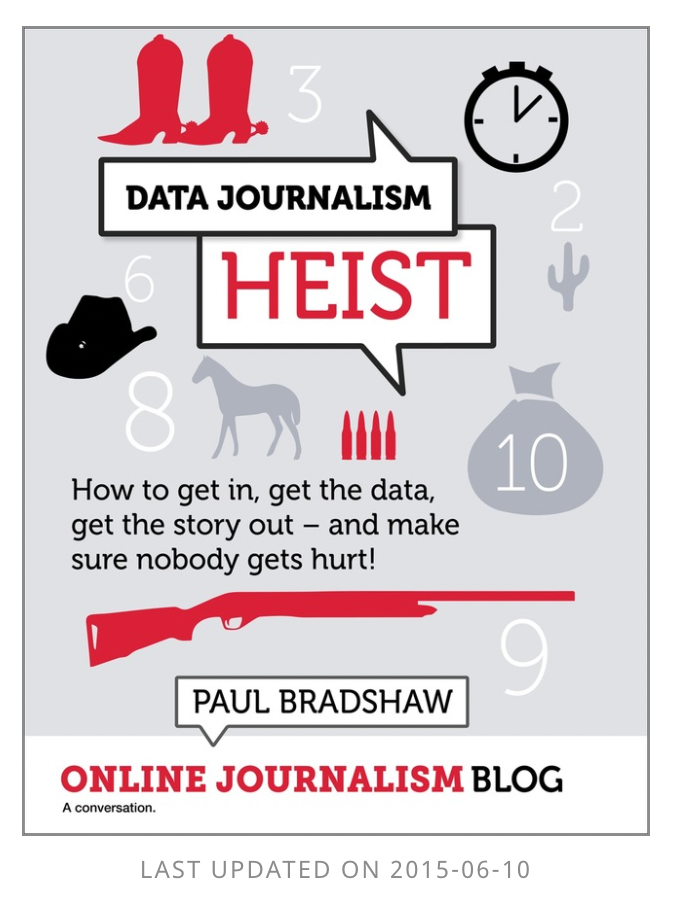
\includegraphics[width=0.9\textwidth,height=\textheight]{./images/start-story-heist.png}

\begin{itemize}
\tightlist
\item
  Compare the claims of powerful people and institutions against facts
  -- the classic investigative approach.
\item
  Report on \emph{unexpected} highs and lows (of change, or of some
  other characteristic)
\item
  Look for outliers -- individual values that buck a trend seen in the
  rest
\item
  Verify or bust some myths
\item
  Find signs of distress, happiness or dishonesty or any other emotion.
\item
  Uncover \emph{new} or \emph{under-reported} long-term trends.
\item
  Find data suggesting your area is \emph{the same} or \emph{different}
  than most others of its kind.
\end{itemize}

Bradshaw also did a recent study of data journalism pieces:
``\href{https://onlinejournalismblog.com/2020/08/11/here-are-the-7-types-of-stories-most-often-found-in-data/}{Here
are the angles journalists use most often to tell the stories in
data}'', in Online Journalism Blog. I'm not sure I agree, only because
he's looking mainly at visualizations rather than stories, but they're
worth considering.

\hypertarget{exercises}{%
\section{Exercises}\label{exercises}}

\begin{itemize}
\item
  If you're a member of Investigative Reporters and Editors, go to the
  site and find a recent prize-winning entry (usually text rather than
  broadcast). Get a copy of the IRE contest entry from the Resources
  page. Try to match up what the reporters said they did and how they
  did it with key portions of the story.
\item
  The next time you find a good data source, try to find a story that
  references it. If your data is local, you might look for a story that
  used similar data elsewhere, such as 911 response times or overdose
  deaths. But many stories use federal datasets that can easily be
  localized. Look at a description of the dataset and then the story to
  see how the data might have been used.
\end{itemize}

\bookmarksetup{startatroot}

\hypertarget{start-math}{%
\chapter{Newsroom math}\label{start-math}}

\begin{quote}
\emph{Statistics are people with the tears washed off}

- Paul Brodeur
\end{quote}

Jo Craven McGinty, then of The New York Times, used simple rates and
ratios to discover that a 6-story brick New Jersey hospital was the most
expensive in the nation. In 2012, Bayonne Medical Center ``charged the
highest amounts in the country for nearly one-quarter of the most common
hospital treatments,'' the
\href{https://www.nytimes.com/2013/05/17/business/bayonne-medical-center-has-highest-us-billing-rates.html}{Times
story said}.

To do this story, McGinty only needed to know the number of the
procedures reported to the government and the total amount each hospital
charged. Dividing those to find an average price, then ranking the most
common procedures, led to this surprising result.

\hypertarget{why-numbers}{%
\section{Why numbers?}\label{why-numbers}}

Using averages, percentages and percent change is the bread and butter
of data journalism, leading to stories ranging from home price
comparisons to school reports and crime trends. It may have been
charming at one time for reporters to announce that they didn't ``do''
math, but no longer. Instead, it is now an announcement that the
reporter can only do some of the job. You will never be able to tackle
complicated, in-depth stories without reviewing basic math.

The good news is that most of the math and statistics you need in a
newsroom isn't nearly as difficult as high school algebra. You learned
it somewhere around the 4th grade. You then had a decade to forget it
before deciding you didn't like math. But mastering this most basic
arithmetic again is a requirement in the modern age.

In working with typical newsroom math, you will need to learn how to:

\begin{itemize}
\tightlist
\item
  Overcome your fear of numbers
\item
  Integrate numbers into your reporting
\item
  Routinely compute averages, differences and rates
\item
  Simplify and select the right numbers for your story
\end{itemize}

While this chapter covers general tips, you can find specific
instructions for typical newsroom math in this
\protect\hyperlink{appendix-math}{Appendix A}

\hypertarget{overcoming-your-fear-of-math}{%
\section{Overcoming your fear of
math}\label{overcoming-your-fear-of-math}}

When we learned to read, we got used to the idea that 26 letters in
American English could be assembled into units that we understand
without thinking -- words, sentences, paragraphs and books. We never got
the same comfort level with 10 digits, and neither did our audience.

Think of your own reaction to seeing a page of words. Now imagine it as
a page of numbers.

Instead, picture the number ``five''. It's easy. It might be fingers or
it might be a team on a basketball court. But it's simple to understand.

Now picture the number 275 million. It's hard. Unfortunately, 275
billion isn't much harder, even though it's magnitudes larger. (A
million seconds goes by in about 11 days but you may not have been alive
for a billion seconds -- about 36 years.)

The easiest way to get used to some numbers is to learn ways to cut them
down to size by calculating rates, ratios or percentages. In your
analysis, keep an eye out for the simplest \emph{accurate} way to
characterize the numbers you want to use. ``Characterize'' is the
important word here -- it's not usually necessary to be overly precise
so long as your story doesn't hinge on a nuanced reading of small
differences. (And is anything that depends on that news? It may not be.)

Here's one example of putting huge numbers in perspective. Pay attention
to what you really can picture - it's probably the \$21 equivalent.

The Chicago hedge fund billionaire Kenneth C. Griffin, for example,
earns about \$68.5 million a month after taxes, according to court
filings made by his wife in their divorce. He has given a total of
\$300,000 to groups backing Republican presidential candidates. That is
a huge sum on its face, yet is the equivalent of only \$21.17 for a
typical American household, according to Congressional Budget Office
data on after-tax income.
\emph{``\href{https://www.nytimes.com/interactive/2015/10/11/us/politics/2016-presidential-election-super-pac-donors.html}{Buying
Power}'', Nicholas Confessore, Sarah Cohen and Karen Yourish, The New
York Times, October 2015}

Originally the reporters had written it even more simply, but editors
found the facts so unbelievable that they wanted give readers a chance
to do the math themselves. That's reasonable, but here's an even simpler
way to say it: ``earned nearly \$1 billion after taxes\ldots He has
given \$300,000 to groups backing candidates, the equivalent of a dinner
at Olive Garden for the typical American family , based on Congressional
Budget Office income data.'' (And yes, the reporter checked the price
for an Olive Garden meal at the time for four people.)

\hypertarget{put-math-in-its-place}{%
\section{Put math in its place}\label{put-math-in-its-place}}

For journalists, numbers -- or facts -- make up the third leg of a stool
supported by human stories or anecdotes, and insightful comment from
experts. They serve us in three ways:

\begin{itemize}
\item
  \textbf{\emph{As summaries}}. Almost by definition, a number counts
  something, averages something, or otherwise summarizes something.
  Sometimes, it does a good job, as in the average height of Americans.
  Sometimes it does a terrible job, as in the average income of
  Americans. Try to find summaries that accurately characterize the real
  world.
\item
  \textbf{\emph{As opinions}}. Sometimes it's an opinion derived after
  years of impartial study. Sometimes it's an opinion tinged with
  partisan or selective choices of facts. Use them accordingly.
\item
  \textbf{\emph{As guesses}}. Sometimes it's a good guess, sometimes
  it's an off-the-cuff guess. And sometimes it's a hopeful guess. Even
  when everything is presumably counted many times, it's still a (very
  nearly accurate) guess. Yes, the ``audits'' of presidential election
  results in several states in 2021 found a handful of errors -- not a
  meaningful number, but a few just the same.
\end{itemize}

Once you find the humanity in your numbers, by cutting them down to size
and relegating them to their proper role, you'll find yourself less
fearful. You'll be able to characterize what you've learned rather than
numb your readers with every number in your notebook. You may even find
that finding facts on your own is fun.

\hypertarget{going-further}{%
\section{Going further}\label{going-further}}

\hypertarget{tipsheets}{%
\subsection*{Tipsheets}\label{tipsheets}}
\addcontentsline{toc}{subsection}{Tipsheets}

\begin{itemize}
\tightlist
\item
  Steve Doig's
  ``\href{https://businessjournalism.org/2017/09/newsroom-math-crib-sheet/}{Math
  Crib Sheet}''
\item
  \protect\hyperlink{appendix-math}{Appendix A}: Common newsroom math,
  adapted from drafts of the book
  \href{https://www.ire.org/product/numbers-in-the-newsroom-using-math-and-statistics-in-news-second-edition-e-version/}{\emph{Numbers
  in the Newsroom}}, by Sarah Cohen.
\end{itemize}

\hypertarget{reading-and-viewing}{%
\subsection*{Reading and viewing}\label{reading-and-viewing}}
\addcontentsline{toc}{subsection}{Reading and viewing}

\begin{itemize}
\item
  ``\href{https://www.poynter.org/news/avoiding-numeric-novocain-writing-well-numbers}{Avoiding
  Numeric Novocain: Writing Well with Numbers},'' by Chip Scanlan,
  Poynter.com
\item
  T. Christian Miller's
  ``\href{https://cronkitedata.s3.amazonaws.com/docs/data-writing-tmiller.pdf}{Writing
  the data-driven story}''
\item
  A viral Twitter thread:
\end{itemize}

\hypertarget{exercises-1}{%
\section{Exercises}\label{exercises-1}}

\begin{itemize}
\tightlist
\item
  Imagine that someone gave you \$1 million and you could spend it on
  anything you want. Write down a list of things that would add up to
  about that amount. That should be easy. Now, imagine someone gave you
  \$1 billion and you could spend it on whatever you want, but anything
  left over after a year had to be returned. How would you spend it?
  (You can give away money, but it can't be more than 50\% of a
  charity's annual revenues. So you can't give 10 \$100 million gifts!)
  See how far you get trying to spend it. A few homes, a few yachts,
  student loan repayments for all of your friends? You've hardly gotten
  started.
\end{itemize}

\bookmarksetup{startatroot}

\hypertarget{start-data-def}{%
\chapter{Defining ``Data''}\label{start-data-def}}

\begin{quote}
data /ˈdeɪ.tə/ :

information in an electronic form that can be stored and used by a
computer, or information, especially facts or numbers, collected to be
examined and \textgreater considered and used to help decision-making

-- Cambridge Dictionary -- sort of \footnote{I flipped the order of
  these two definitions!}
\end{quote}

\hypertarget{the-birth-of-a-dataset}{%
\section{The birth of a dataset}\label{the-birth-of-a-dataset}}

Most journalism uses data collected for one purpose for something
entirely different. Understanding its original uses -- what matters to
the people who collected it, and what doesn't -- will profoundly affect
its accuracy or usefulness.

\hypertarget{trace-data-and-administrative-records}{%
\subsection*{Trace data and administrative
records}\label{trace-data-and-administrative-records}}
\addcontentsline{toc}{subsection}{Trace data and administrative records}

In
``\href{https://www.amazon.com/Art-Access-Strategies-Acquiring-Records/dp/1604265507}{The
Art of Access}'', David Cullier and Charles N. Davis describe a process
of tracking down the life and times of a dataset. Their purpose is to
make sure they know how to request it from a government agency. The same
idea applies to using data that we acquire elsewhere.

Understanding how and why data exists is crucial to understanding what
you, as a reporter, might do with it.

Anything you can systematically search or analyze could be considered
one piece of of data. As reporters, we usually deal with data that was
created in the process of doing something else -- conducting an
inspection, delivering a tweet, or scoring a musical. In the sciences,
this flotsam and jetsom that is left behind is called ``digital trace
data'' if it was born digitally.

In journalism and in the social sciences, many of our data sources were
born during some government process -- a safety inspection, a traffic
ticket, or the filing of a death certificate. These administrative
records form the basis of much investigative reporting and they are
often the subject of public records and FOIA requests. They were born as
part of the government doing its job, without any thought given to how
it might be used in another way. In the sciences, those are often called
``administrative records''.

This trace data might be considered the first part of the definition
above -- information that can be stored and used.

Here's how Chris Bail from Duke University
\href{https://www.youtube.com/embed/uuSWQN7uYhk}{describes it}.

\hypertarget{data-collected-and-curated-for-analysis}{%
\subsection*{Data collected and curated for
analysis}\label{data-collected-and-curated-for-analysis}}
\addcontentsline{toc}{subsection}{Data collected and curated for
analysis}

Another kind of data is that which is compiled or collected specifically
for the purpose of studying something. It might collected in the form of
a survey or a poll, or it might be a system of sampling to measure
pollution or weather. But it's there because the information has
intrinsic value AS information.

The video suggests a hard line between trace data and custom data. In
practice, it's not that clear. Many newsrooms may curate data published
in other sources or in administrative records, such as the Washington
Post's police shooting dataset. In other cases, the agencies we are
covering get already-compiled data from state and local governments.

This type of data might be considered the second type in the definition
-- tabular information that is used for decision-making.

\hypertarget{granular-and-aggregated-data}{%
\section{Granular and aggregated
data}\label{granular-and-aggregated-data}}

One of the hardest concepts for a lot of new data journalists is the
idea of \emph{granularity} of your data source. There are a lot of ways
to think about this: individual items in a list vs.~figures in a table;
original records vs.~compilations; granular data vs.~statistics.

Generally, an investigative reporter is interested in getting data that
is as close as possible to the most granular information that exists, at
least on computer files. Here's an example, which might give you a
little intuition about why it's so important to think this way:

When someone dies in the US, a standard death certificate is filled out
by a series of officials - the attending physician, the institution
where they died and even the funeral direcor.

\href{https://www.cdc.gov/nchs/data/dvs/death11-03final-acc.pdf}{Click
on this link} to see a blank version of the standard US death
certificate form -- notice the detail and the detailed instructions on
how it is supposed to be filled out. \footnote{You should do this
  whenever you get a dataset created from administrative records. That
  is, track down its origin and examine the pieces you were given and
  the pieces that were left out; look at what is written in free-form vs
  what is presented as a check box. You may need a copy of the template
  that an agency uses to collect the information, but many governments
  make these available on their websites or are willing to provide them
  without a fuss.}

A good reporter could imagine many stories coming out of these little
boxes. Limiting yourself to just to COVID-19-related stories: You could
profile the local doctor who signed the most COVID-19-related death
certificates in their city, or examine the number of deaths that had
COVID as a contributing, but not underlying or immediate, cause of
death. You could compare smoking rates in the city with the number of
decedents whose tobacco use likely contributed to their death. Maybe
you'd want to know how long patients suffered with the disease before
they died. And you could map the deaths to find the block in your town
most devastated by the virus.

Early in the pandemic, Coulter Jones and Jon Kamp examined the records
from one of the few states that makes them public, and concluded that
``\href{https://www.wsj.com/articles/coronavirus-deaths-were-likely-missed-in-michigan-death-certificates-suggest-11590073280\%5D\%20\%5E\%5BWall\%20Street\%20Journal,\%20May\%2021,\%202020}{Coronavirus
Deaths were Likely Missed in Michigan, Death Certificates Suggest}''

But you probably can't do that. The reason is that, in most states,
death certificates are not public records and are treated as secrets.
\footnote{See
  ``\href{https://www.researchgate.net/publication/348322257_Secrecy_in_Death_Records_A_Call_to_Action}{Secrecy
  in Death Records: A call to action}'', by Megain Craig and Madeleine
  Davison, Journal of Civic Information, December 2020}. Instead, state
and local governments provide limited statistics related to the deaths,
usually by county, with no detail. That's the difference between
granular data and aggregate data. Here are some of the typical (not
universal) characteristics of each:

\begin{longtable}[]{@{}
  >{\raggedright\arraybackslash}p{(\columnwidth - 2\tabcolsep) * \real{0.5000}}
  >{\raggedright\arraybackslash}p{(\columnwidth - 2\tabcolsep) * \real{0.5000}}@{}}
\toprule()
\begin{minipage}[b]{\linewidth}\raggedright
Granular
\end{minipage} & \begin{minipage}[b]{\linewidth}\raggedright
Aggregate
\end{minipage} \\
\midrule()
\endhead
Intended for some purpose other than your work & Intended to be
presented as is to the public \\
Many rows (records), few columns (variables) & Many columns (variables),
few rows (records) \\
Requires a good understanding of the source & Explanatory notes usually
come with the data \\
Easy to cross-reference and compile & Often impossible to repurpose \\
Has few numeric columns & May be almost entirely numerical \\
Is intended for use in a database & Is intended for use in a
spreadsheet \\
\bottomrule()
\end{longtable}

We often have to consider the trade-offs. Granular data with the detail
we need - especially when it involves personally identifiable
information like names and addresses - can take months or years of
negotiation over public records requests, even when the law allows it.
It's often much easier to convince an agency to provide summarized or
incomplete data. Don't balk at using it if it works for you. But
understand that in the vast majority of cases, it's been summarized in a
way that's lost information that could be important to your story.

\hypertarget{nouns}{%
\section{Nouns}\label{nouns}}

That brings us to one of the most important things you must find out
about any data you begin to analyze: What ``noun'' does each row in a
tabular dataset represent? In statistics, they might be called
\emph{observations} or \emph{cases}. In data science, they're usually
called \emph{records}. Either way, every row must represent the same
thing -- a person, a place, a year, a water sample or a school. And you
can't really do anything with it until you figure out what that is.

In 2015, Sarah Cohen did a story at The New York Times called
\href{https://www.nytimes.com/2014/04/07/us/more-deportations-follow-minor-crimes-data-shows.html}{``More
Deportation Follow Minor Crimes, Records Show''}. The government had
claimed it was only removing hardened criminals from the country, but
our analysis of the data suggested that many of them were for minor
infractions.

In writing the piece, they had to work around a problem in our data: the
agency refused to provide them anything that would help us distinguish
individuals from one another. All the reporters knew was that each row
represented one deportation -- not one person! Without a column, or
\emph{field} or a \emph{variable} or an \emph{attribute} for an
individual -- say, name and date of birth, or some scrambled version of
an their DHS number -- they had no way to even estimate how often people
were deported multiple times. If you read the story, you'll see the very
careful wording, except when they had reported out and spoken to people
on the ground.

\hypertarget{further-reading}{%
\section{Further reading}\label{further-reading}}

\begin{itemize}
\item
  \href{https://datajournalism.com/read/handbook/one/understanding-data/basic-steps-in-working-with-data}{``Basic
  steps in working with data''}, the Data Journalism Handbook, Steve
  Doig, ASU Professor. He describes in this piece the problem of not
  knowing exactly how the data was compiled.
\item
  ``\href{https://www.nytimes.com/2020/07/08/podcasts/the-daily/coronavirus-data-united-states.html}{Counting
  the Infected}'' , Rob Gebellof on The Daily, July 8, 2020.
\item
  ``\href{https://eagereyes.org/basics/spreadsheet-thinking-vs-database-thinking}{Spreadsheet
  thinking vs.~Database thinking}'', by Robert Kosara, gets at the idea
  that looking at individual items is often a ``database'', and
  statistical compilations are often ``spreadsheets''.
\item
  ``\href{https://vita.had.co.nz/papers/tidy-data.pdf}{Tidy Data}'', in
  the Journal of Statistical Software (linked here in a pre-print) by
  Hadley Wickham , is the quintessential article on describing what we
  think of as ``clean'' data. For our purposes, much of what he
  describes as ``tidy'' comes when we have individual, granular records
  -- not statistical compilations. It's an academic article, but it has
  the underlying concepts that we'll be working with all year.
\end{itemize}

\hypertarget{exercises-2}{%
\section{Exercises}\label{exercises-2}}

\begin{itemize}
\tightlist
\item
  The next time you get a government statistical report, scour all of
  the footnotes to find some explanation of where the data came from.
  You'll be surprised how often they are compilations of administrative
  records - the government version of trace data.
\end{itemize}

\bookmarksetup{startatroot}

\hypertarget{introduction-1}{%
\chapter{Introduction}\label{introduction-1}}

Some people consider using spreadsheets the table stakes for getting
into data journalism. It's relatively easy to see what you're doing and
you can easily share your work with your colleagues. In fact, pieces of
the
\href{https://www.pulitzer.org/winners/new-york-times-6}{Pulitzer-Prize
winning COVID-19 coverage} from The New York Times was compiled using an
elaborate and highly tuned set of Google spreadsheets with dozens of
contributors.

This guide uses Google Sheets, although you should be able to do these
exercises with Excel on the Mac or Windows. Excel on the Mac is pretty
good, bu Excel in Windows is very different -- it has much more
capability for working with large and more complex data, and provides
better tuning for import and other operations. There is a table that
compares keystrokes for Apple desktops, laptops and Windows machines for
Excel at the bottom of \href{xl-refresher}{An Excel Refresher}

\hypertarget{tutorials}{%
\section{Tutorials}\label{tutorials}}

Spreadsheets in the form of Google Sheets or Excel are used in almost
every workplace in America. This section covers most of what you need in
the newsroom, which is a different set of skills than in other
businesses.

\begin{itemize}
\item
  \href{xl-refresher.html}{An Excel Refresher} : Start over with good
  habits
\item
  \href{xl-filter-sort.html}{Sorting and filtering to find stories} :
  The first step of interviewing data
\item
  \href{xl-pivot.html}{Grouping with pivot tables}: Aggregating, and the
  super power of spreadsheets
\item
  \href{xl-formulas.html}{Formulas in Excel}: Percents, sums, and other
  basic computations used in newsrooms.
\end{itemize}

\hypertarget{practice-exercises}{%
\section{Practice exercises}\label{practice-exercises}}

\begin{itemize}
\tightlist
\item
  \href{xl-practice-noc.html}{Practice with ``notice of claims'' from
  Phoenix}: Filtering and pivot table practice using claims made against
  the city of Phoenix 2010-2020.
\end{itemize}

\bookmarksetup{startatroot}

\hypertarget{an-excel-refresher}{%
\chapter{An Excel Refresher}\label{an-excel-refresher}}

Spreadsheets are everywhere, so it's worth re-learning how to use them
well. Reporters usually use spreadsheets in three ways:

\begin{itemize}
\item
  To create original databases of events for sorting, filtering and
  counting. Examples include a long-running court case; the details of
  each opioid death in a city; a list of police shootings and their
  documents; or even a list of your own public records requests or
  contact log.
\item
  To use data created by others for fast, simple analysis and data
  cleanup. Many government agencies provide their information in
  spreadsheet form, but they often require some rejiggering before you
  can use them.
\item
  To perform simple, straightforward analysis on data and share with
  team members. This is becoming less common as more reporters learn
  programming languages, but it's still common in newsrooms to share
  data, especially through Google Sheets.
\end{itemize}

(This guide is done using a Mac. Windows machines will be a little
different, mainly because you'll have more choices in most menus. The
Mac CMD key is the same as the Windows CNTL key.)

Some reporters flinch at typing in 30 or 100 entries into a spreadsheet.
You shouldn't. If you learn to take notes in a structured way, you'll
always be able to find and verify your work. If you try to calculate a
sum of 30 numbers on a calculator, you'll have to type them all in at
least twice anyway. Also, getting used to these easy tasks on a
spreadsheet keeps your muscles trained for when you need to do more.

\hypertarget{re-learning-sheets-from-the-ground-up}{%
\section{Re-learning Sheets from the ground
up}\label{re-learning-sheets-from-the-ground-up}}

\hypertarget{the-spreadsheet-grid}{%
\subsection{The spreadsheet grid}\label{the-spreadsheet-grid}}

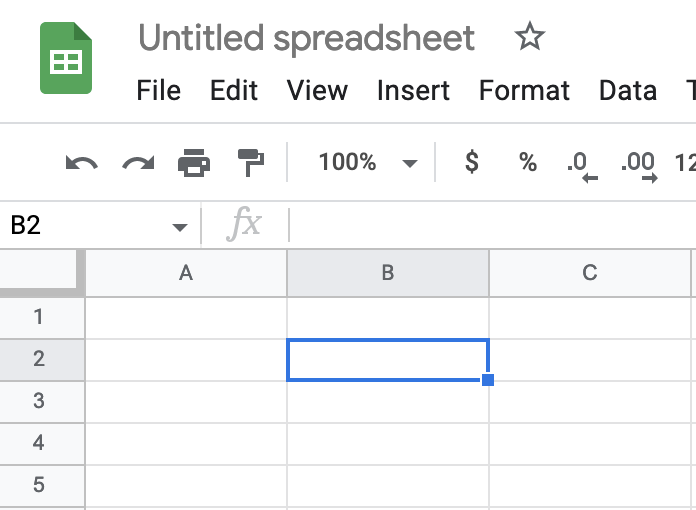
\includegraphics{./images/sheets-refresher-battleship.png}

When you start up a spreadsheet (try entering sheet.new into your
browser!), you'll see letters across the top and numbers down the side.
If you ever played Battleship, you'll recognize the idea -- every little
square, or cell, is referenced by the intersection of its column letter
and row number:

B2 is the cell that is currently active. You can tell because it's
outlined in the sheet and it's shown on the upper left corner.

\hypertarget{mouse-shapes}{%
\subsection{Mouse shapes}\label{mouse-shapes}}

\begin{longtable}[]{@{}
  >{\raggedright\arraybackslash}p{(\columnwidth - 2\tabcolsep) * \real{0.7500}}
  >{\raggedright\arraybackslash}p{(\columnwidth - 2\tabcolsep) * \real{0.2500}}@{}}
\toprule()
\endhead
\textbf{The Copy Tool}, or the thin black cross. When you see this,
you'll copy anything that's selected. This can be good or bad. &
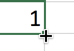
\includegraphics{./images/xl-refresher-copy.png} \\
\textbf{The Evil Hand}. (In Windows, this is the Evil Arrow). If you use
this symbol, you will MOVE the selection to a new location. This is very
rarely a good idea or something you intend. &
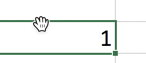
\includegraphics{./images/xl-refresher-evilhand.png} \\
\bottomrule()
\end{longtable}

\hypertarget{selecting-cells-and-ranges}{%
\subsection{Selecting cells and
ranges}\label{selecting-cells-and-ranges}}

Spreadsheets act only on the cells or regions you have selected. If you
begin typing, you'll start entering information into the currently
selected cell.

To select: Hold the BFWPS over the cell and clice ONCE -- \emph{not
twice}. Check the formula bar to make sure you've selected what you
think you've got. You can also look at the bottom right of your
spreadsheet for more information.

You'll often work with \emph{ranges} of cells in formulas. These are
defined by the corners of the area you want to work on -- often a column
of information. In the example below, the range is A1:B6, with the ``:''
referring to the word ``through''.

\emph{To select a group of cells and act on them all at once}: Hover the
BFWPS over one corner, click ONCE and drag to the diagonal corner. Make
sure the Evil Hand is nowhere to be seen. The entire area will be shaded
in except for the currently selected cell. Look at the upper right
corner to see how many rows and columns you selected.

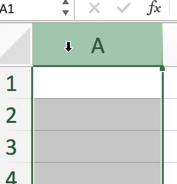
\includegraphics{./images/xl-refresher-columnselect.png}

\emph{To select a column or row} : Hover the cursor over the letter at
the top of the column. For a row, hover it over the row number in the
margin

\hypertarget{reading-the-screen}{%
\subsection{Reading the screen}\label{reading-the-screen}}

The areas of the spreadsheet have different visual clues, and learning
to read them will make your life much easier.

\hypertarget{entering-data}{%
\subsection{Entering data}\label{entering-data}}

Select the cell and start typing. The information you type won't be
locked into the cell until you hit the Return / Enter key, or move your
selection to another cell. Hit ``Escape'' to cancel the entry.

You can't do a lot of things while you're editing, so if you have a lot
of greyed out menu items, look at your formula bar to see if you are
still editing a cell.

If you're having trouble getting to a menu item or seeing the result of
your work, try hitting ``Escape'' and try again. You may not have
actually entered the information into the sheet.

\hypertarget{locking-in-headings}{%
\subsection{Locking in headings}\label{locking-in-headings}}

As your spreadsheet grows vertically with more rows, you'll want to be
able to see the top all the time. When it grows horizontally with more
columns, you'll probably want to see columns in the left, such as names.
This is called ``Freezing Panes'' -- you freeze part of the page so it
stays in place when you move around.

In Google Sheets, this is done via the View -\textgreater{} Freeze menu:

\begin{figure}

{\centering 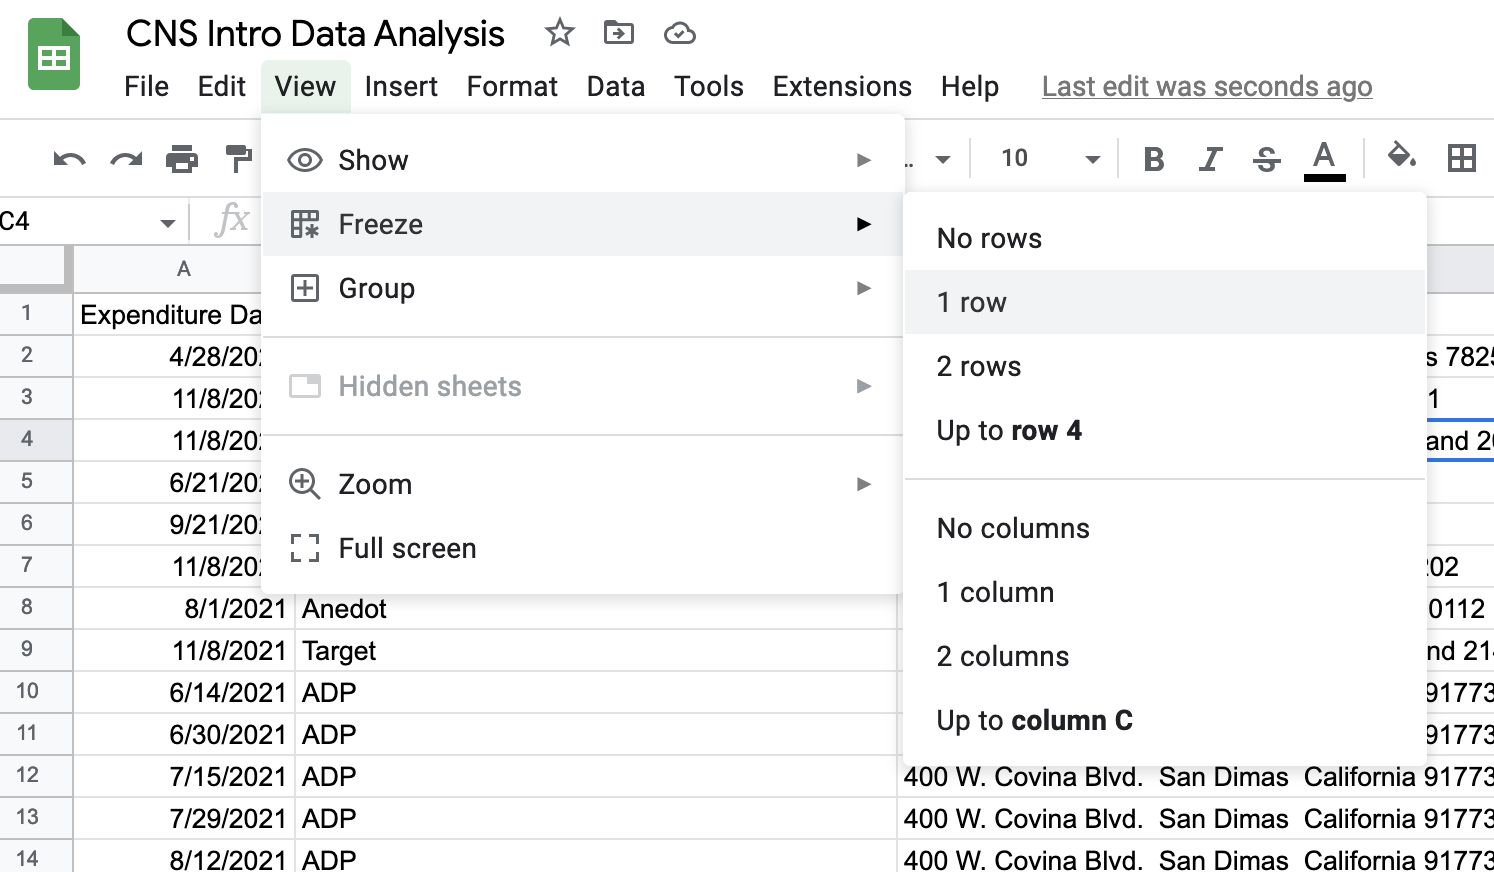
\includegraphics[width=1\textwidth,height=\textheight]{./images/sheets-refresher-freezepanes.png}

}

\caption{freeze panes}

\end{figure}

\hypertarget{formatting-tricks}{%
\subsection{Formatting tricks}\label{formatting-tricks}}

\begin{itemize}
\item
  Use the buttons or the format dialog box to make numbers easier to
  read.
\item
  If a column is filled with a lot of text, select the column and look
  on the Home ribbon next to the formatting area for ``Wrap Text''. This
  means that when you double-click to widen a column, it will get
  taller, not wider. This is good when you need to save valuable real
  estate on the screen.
\end{itemize}

\hypertarget{getting-started-with-a-dataset}{%
\section{Getting started with a
dataset}\label{getting-started-with-a-dataset}}

\textbf{SLOW DOWN!} Don't do anything until you understand what you have
in front of you and can predict what your next mouse click will do to
it.

Most data we encounter was created by someone else for some purpose
other than ours. This means that you can't assume anything. It may not
be complete. It may be inaccurate. It may mean something completely
different than it appears at first blush.

\hypertarget{first-steps}{%
\subsection{First steps}\label{first-steps}}

\begin{itemize}
\tightlist
\item
  Document where you got the spreadsheet and how you can get back to the
  original.
\item
  Read anything you can about what it contains. Look for documentation
  that comes with the data.
\item
  Save the original into a safe place with its original name and
  metadata. Work on a copy.
\item
  If the spreadsheet shows \#\#\#\# instead of words or numbers, widen
  your columns. If it shows 7E-14 or something like that, format them as
  numbers, not ``General''.
\item
  Check your corners -- look at the top left and bottom right. Is the
  data all in one area? Are there footnotes or other non-data sections
  mixed in? We're going to want to fix that later.
\end{itemize}

\hypertarget{interview-your-data}{%
\subsection{Interview your data}\label{interview-your-data}}

\hypertarget{headings}{%
\subsubsection{Headings}\label{headings}}

The most fraught part of data reporting is understanding what each
\emph{column} actually means. These often have cryptic, bureaucratic
names. You may need to go back to the source of the data to be sure you
actually understand them.

If your data doesn't have any headings, that's going to be your first
priority. In effect, you'll need to build what we call a \emph{data
dictionary} or \emph{record layout} if one hasn't been provided. Many
reporters create these as a page in a dataset.

\hypertarget{unit-of-analysis}{%
\subsubsection{Unit of analysis}\label{unit-of-analysis}}

A \emph{unit of analysis} refers to the items that are listed in the
rows of your dataset. Ideally, every row should be at the same unit of
analysis -- a person, an inspection, or a city, for example. Summaries
should be separated by a blank row, or moved to a different sheet. Think
of this as the noun you'd use to describe every row.

\hypertarget{row-numbers}{%
\subsubsection{Row numbers}\label{row-numbers}}

The data was probably given to you in some sort of natural sort order.
Different computer systems sort differently -- some are case-sensitive,
others are not. It may depend on when and where the data as created! The
order of the data may even depend on a column you don't have. If you
don't do something now, you'll never be able to get back to the original
order, which could have meaning for both the agency and for
fact-checking.

\bookmarksetup{startatroot}

\hypertarget{sorting-and-filtering-to-find-stories}{%
\chapter{Sorting and filtering to find
stories}\label{sorting-and-filtering-to-find-stories}}

\hypertarget{a-sorting-miracle}{%
\section{A sorting miracle}\label{a-sorting-miracle}}

When Stephen Neukam - who was sitting in this class a year ago - wanted
to find out who was funding candidates for Maryland's open governor's
seat this year, he downloaded data from the State Board of Elections
that listed contributions to the wide array of hopefuls seeking to
replace Larry Hogan in Annapolis.

He wasn't sure at first what he was looking for, so he started the way
that many reporters do with data: by sorting and filtering. Were there
outliers in the list of contributions, and which candidates were getting
their money from unusual (non-Maryland) sources?

Neukam quickly found his story: in the race to be governor, Maryland
candidates, and in particular Wes Moore, a first-time Democratic
candidate, were raising millions of dollars from out of state donors.

The story,
``\href{https://cnsmaryland.org/2022/03/03/millions-in-out-of-state-donations-help-fuel-high-profile-maryland-democratic-governor-candidates/}{Millions
in out-of-state donations help fuel high-profile Maryland Democratic
governor candidates}'' helped explain where candidates were going to
fund one of the most contested primaries in recent history (Moore ended
up winning).

\hypertarget{sorting-and-filtering-as-a-reporting-tool}{%
\section{Sorting and filtering as a reporting
tool}\label{sorting-and-filtering-as-a-reporting-tool}}

Sorting and filtering can:

\begin{itemize}
\tightlist
\item
  Narrow your focus to specific items that you want to examine in your
  story.
\item
  Show you rows containing the highest and lowest values of any column.
  That can be news or it can be errors or other problems with the data.
\item
  Let you answer quick ``how many?'' questions, with a count of the rows
  that match your criteria. (In the next lesson, you'll see that pivot
  tables, or group-by queries, are much more powerful for this in most
  cases.)
\end{itemize}

\hypertarget{example-data}{%
\section{Example data}\label{example-data}}

::: \{.alert .alert-info \} -
\href{https://github.com/stephenneukam/CNS_Annapolis/tree/main/Campaign_finance}{Data
from the State Board of Elections} for use in this tutorial -
\href{https://campaignfinance.maryland.gov/Public/ViewReceiptsMain}{Documentation
from the SBOE's site} :::

\begin{itemize}
\item
  The data for this is from the Maryland State Board of Elections's
  Campaign Finance Database. There are a couple of caveats:
\item
  It includes money raised as of Jan.~12, 2022, which covers all of
  2021.
\item
  These are self-reported by campaigns, and subject to amendment in case
  of errors or omissions.
\end{itemize}

The original data download link for Wes Moore's contributions is
\url{https://github.com/stephenneukam/CNS_Annapolis/raw/main/Campaign_finance/Moore_ContributionsList.csv}.
Download it to your computer and then, in a browser, type sheet.new to
create a new Google Sheet. From there, use File -\textgreater{} Import
and choose ``Upload'' and select the file on your computer. Click the
``Import Data'' button when it appears. Then give your sheet a name,
like ``Wes Moore Contributions''.

It's a good example set for us because it's been used as the basis of
Neukam's story and it has at least one of each \emph{data type} that we
plan to deal with in Google Sheets or Excel. And, critically, the first
row contains headers, not data. Always have headers, even if you have to
add them.

\hypertarget{understanding-data-types}{%
\section{Understanding data types}\label{understanding-data-types}}

When you open the spreadsheet, the first thing to notice is its
\href{start-data-def.html}{\emph{granularity}}. Unlike Census or budget
spreadsheets, this is a list capturing specific characteristics of each
contribution. Each column has the same \emph{type} of data from top to
bottom. Those types are:

\begin{itemize}
\item
  \textbf{Text}. Text or ``character'' columns can come in long or short
  form. When they are standardized (the values can contain only one of a
  small list of values), they're called ``categorical''. If they're more
  free-form, they're might be called ``free text''. The computer doesn't
  know the difference, but you should. The Post data has examples of
  both. In spreadsheets, text is left-justified (they move toward the
  left of the cell and will line up vertically at the beginning)
\item
  \textbf{Numbers}. These are pure numbers with no commas, dollar signs
  or other embellishments. In Google Sheets these can be formatted to
  \emph{look} like numbers in different ways, but underneath they're
  just numbers. Adding up a column of numbers that has a word in it or
  has missing values will just be ignored. It will trip up most other
  languages. These are right-justified, so the last digit is always
  lined up vertically.
\item
  \textbf{Logical}: This is a subset of text. It can take one of only
  two values -- yes or no, true or false. There is no ``maybe''.
\item
  \textbf{Date and times}: These are actual dates on the calendar, which
  have magical properties. Underneath, they are a number. In Google
  Sheets and Excel, that number is the number of days since Jan.~1,
  1900.\footnote{Each language deals with dates and times a little
    differently. We'll see how R does it later on. But just know that
    dates can be tricky because of these differences and
    \href{https://infiniteundo.com/post/25326999628/falsehoods-programmers-believe-about-time}{time
    is even more tricky}} They can also have time attached to them,
  which is a fraction of a day. What this means is that the number
  44,536.5 is really Dec.~6, 2021 at noon. In Sheets, you use a format
  to tell the spreadsheet how you want to see the date or time, just the
  way you look at dollar values with commas and symbols. (If you get a
  spreadsheet with a lot of dates of 1/1/1900, it means there is a 0 in
  that column, which is sometimes a fill-in for ``I don't know.'')
\end{itemize}

Here's a picture of a date that is shown in a variety of formats.

\begin{figure}

{\centering 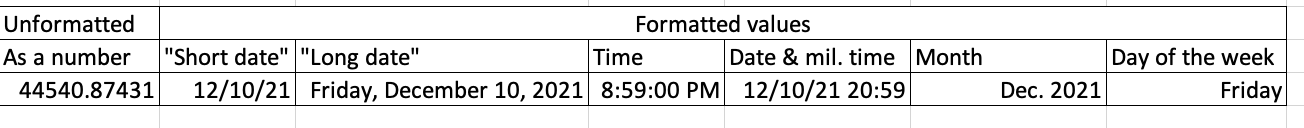
\includegraphics[width=1\textwidth,height=\textheight]{./images/xl-filter-sort-dates.png}

}

\caption{date formats}

\end{figure}

All of these are the same, underlying value -- the number at the left.
Notice that all of these are right-justified.

This means that when you see ``Friday, December 10'', the computer sees
44540.87431. When you put the dates in order, they won't be alphabetized
with all of the Fridays shown together. Instead, they'll be arranged by
the actual date and time.

It also means that you can compute 911 response times even when it
crosses midnight, or or compute the someone's age today given a date of
birth. Keeping actual calendar dates in your data will give it much more
power than just having the words. (Sheets and Excel use the 1st of the
month as a stand-in for an actual date when all you know is the month
and year.)

\hypertarget{sorting-rows}{%
\subsection{Sorting rows}\label{sorting-rows}}

Sorting means rearranging the rows of a data table into a different
order. Some reporters take a conceptual shortcut and call this ``sorting
columns''. That thinking will only get you into trouble -- it lets you
forget that you want to keep the rows in tact while changing the order
in which you see them. In fact, in other languages it's called ``order
by'' or ``arrange'' by one or more columns -- a much clearer way to
think of it.

To sort in Google Sheets, first highlight the entire sheet by clicking
on the button above the first row and to the left of the first column.
So, between the 1 and the A. Then, look for the sort options under the
Data drop-down menu at the top of your screen, and choose ``Sort Range''
and then ``Advanced range sorting options''. Trust me, this is how you
want to do it. Check the box that says ``Data has header row'' and Sort
by Contribution Date. In this case, sorting from A to Z gives you a list
of the contributions in chronological order.

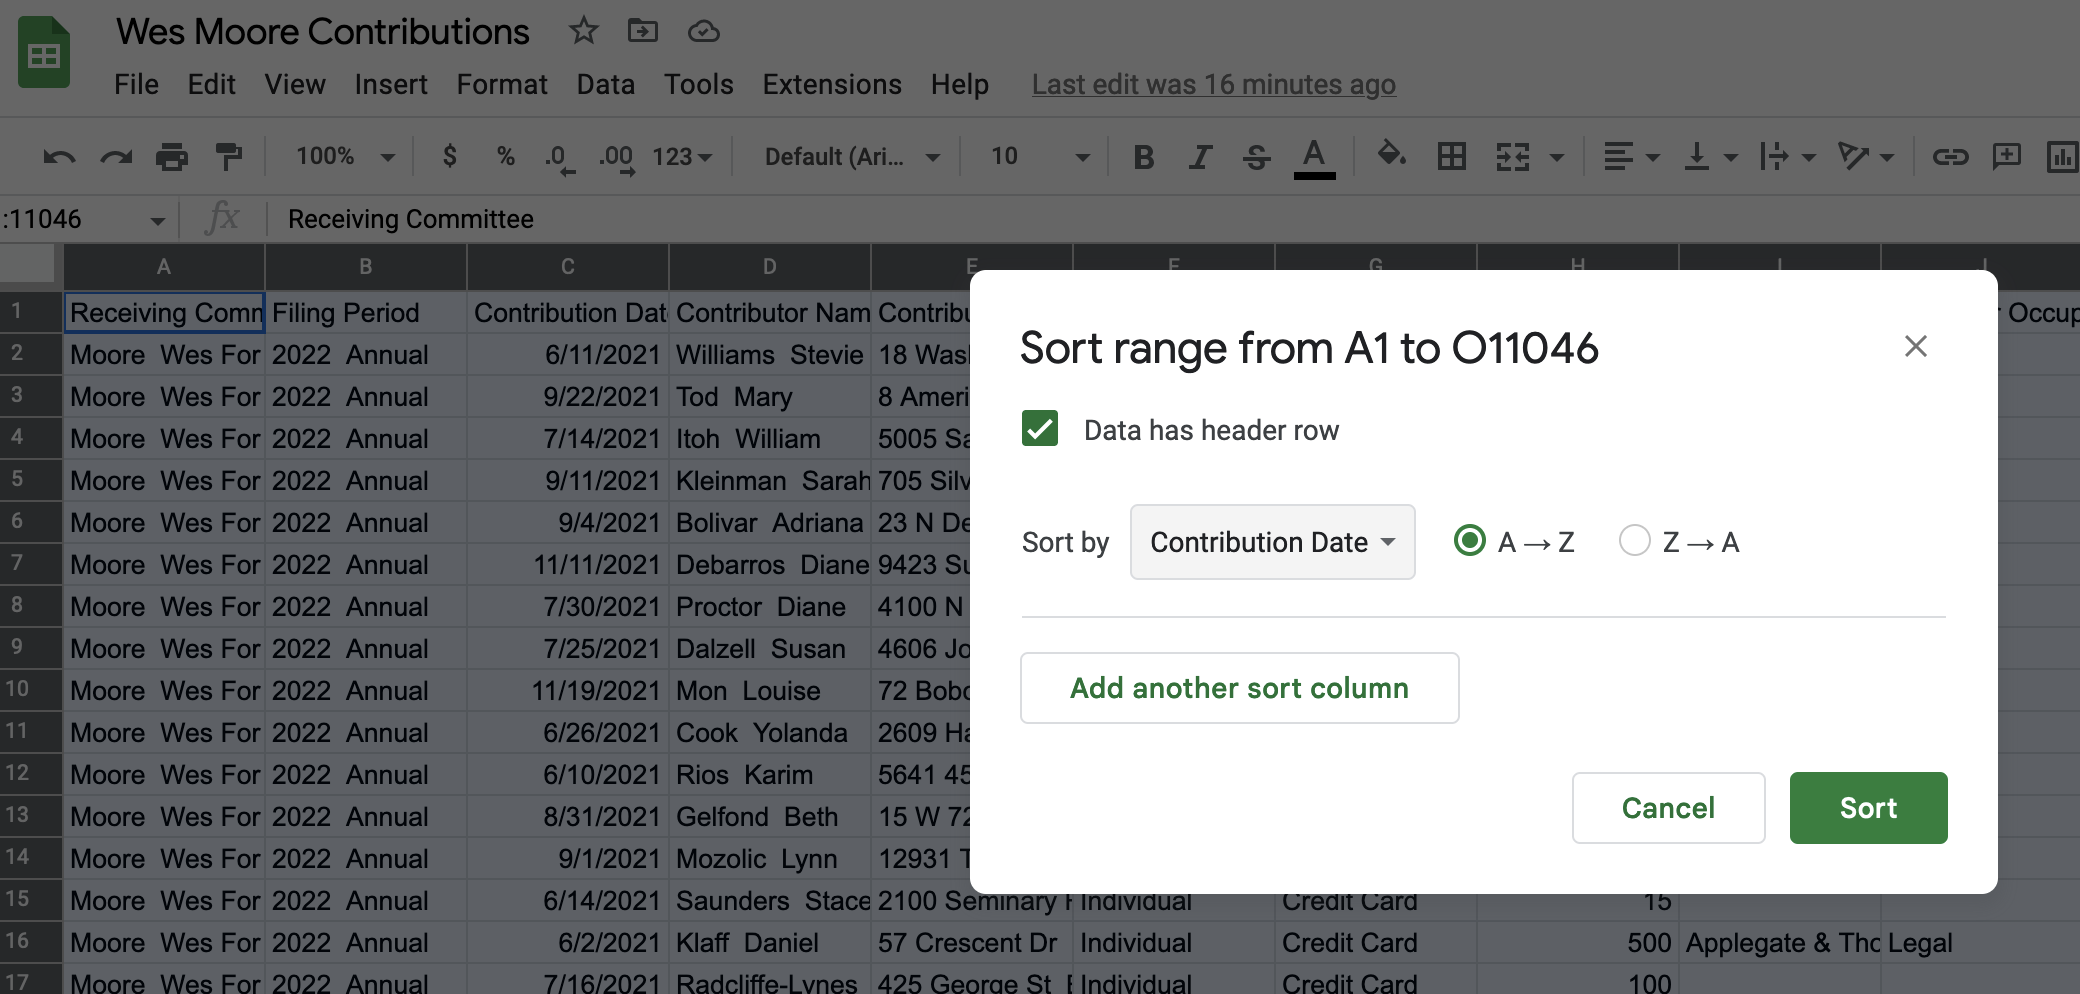
\includegraphics[width=0.8\textwidth,height=\textheight]{./images/sheets-filter-sort-sortbox.png}

\hypertarget{adding-fields-to-the-sort}{%
\subsubsection*{Adding fields to the
sort}\label{adding-fields-to-the-sort}}
\addcontentsline{toc}{subsubsection}{Adding fields to the sort}

Adding more columns to the sort box tells Sheets what to do when the
first one is the same or tied. For example, sorting first by date then
by amount gives you a list that shows all of the contributions by date
in sequence:

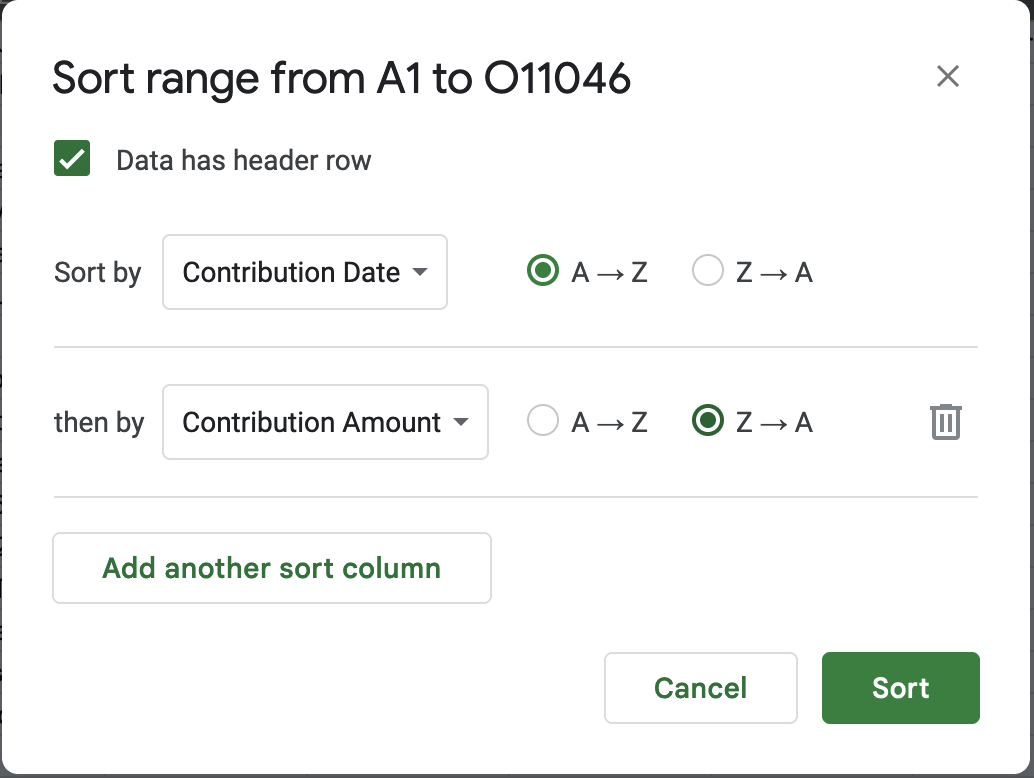
\includegraphics[width=0.5\textwidth,height=\textheight]{./images/sheets-filter-sort-date.png}

\hypertarget{filtering}{%
\subsection{Filtering}\label{filtering}}

Filtering means picking out only some of the rows you want to see based
on a criteria you select in a column. Think of it as casting a fishing
net -- the more filters you add, the fewer fish will be caught.

To turn on filters in Google Sheets, go to Data -\textgreater{} Create a
filter. It will add small down arrows to each column in the first row,
another reason why headers are crucial. You can filter by multiple
columns, and each filter you select adds more conditions, narrowing your
net.

To find contributions of \$5,000, use the drop-down menu under
\texttt{Contribution\ Amount} to select it and hit ``OK''.

When you do this, notice that the drop-down arrow has turned into a
solid green funnel and that any rows that don't match your filter are
hidden.

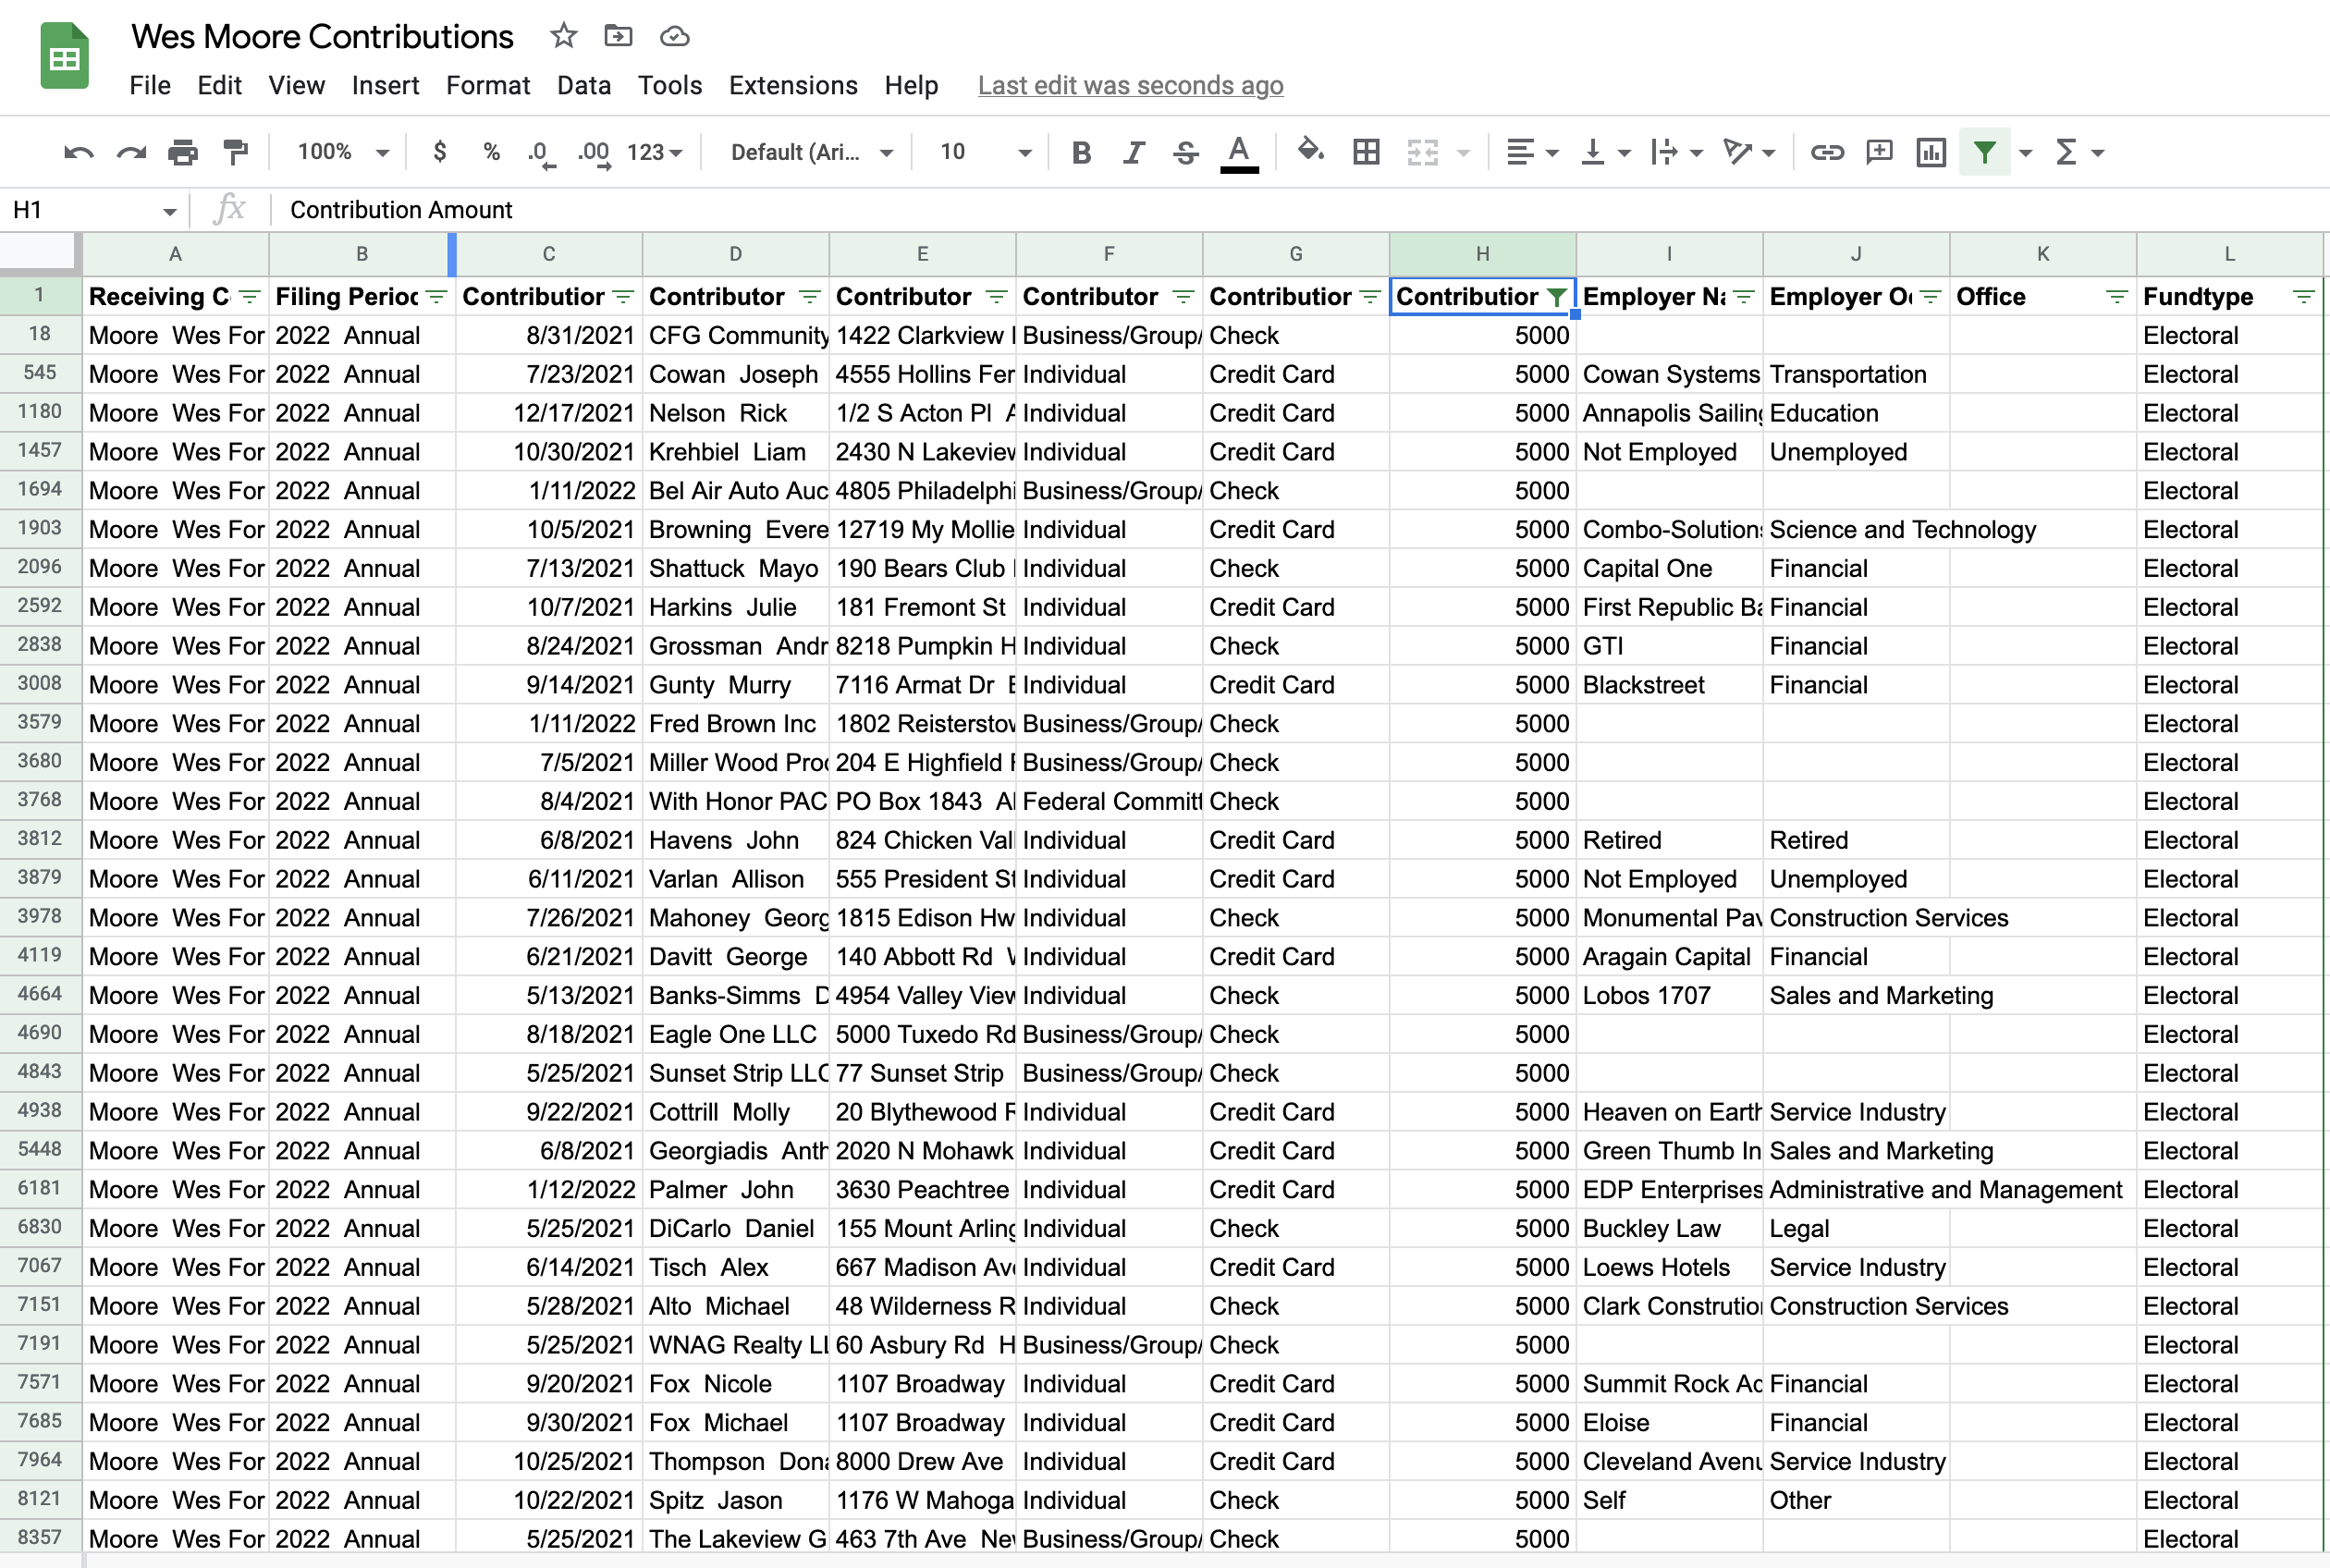
\includegraphics{./images/sheets-filter-sort-onefilter.png}

This method works for small-ish and simple-ish columns. If your column
has more than 10,000 different entries, such as names or addresses, only
the first 10,000 will be considered. We only caught these for stories
when someone did a fact-check using a different method of filtering. If
your column has a lot of distinct entries, use option that says ``Choose
One'', and then use the ``Contains'' option. Better yet, don't use
filtering for counting things at all.

Add more filters to narrow down your list of cases even more. For
example, if you wanted to see \$5,000 contributions from individuals,
you would choose ``Individual'' under Contributor Type:

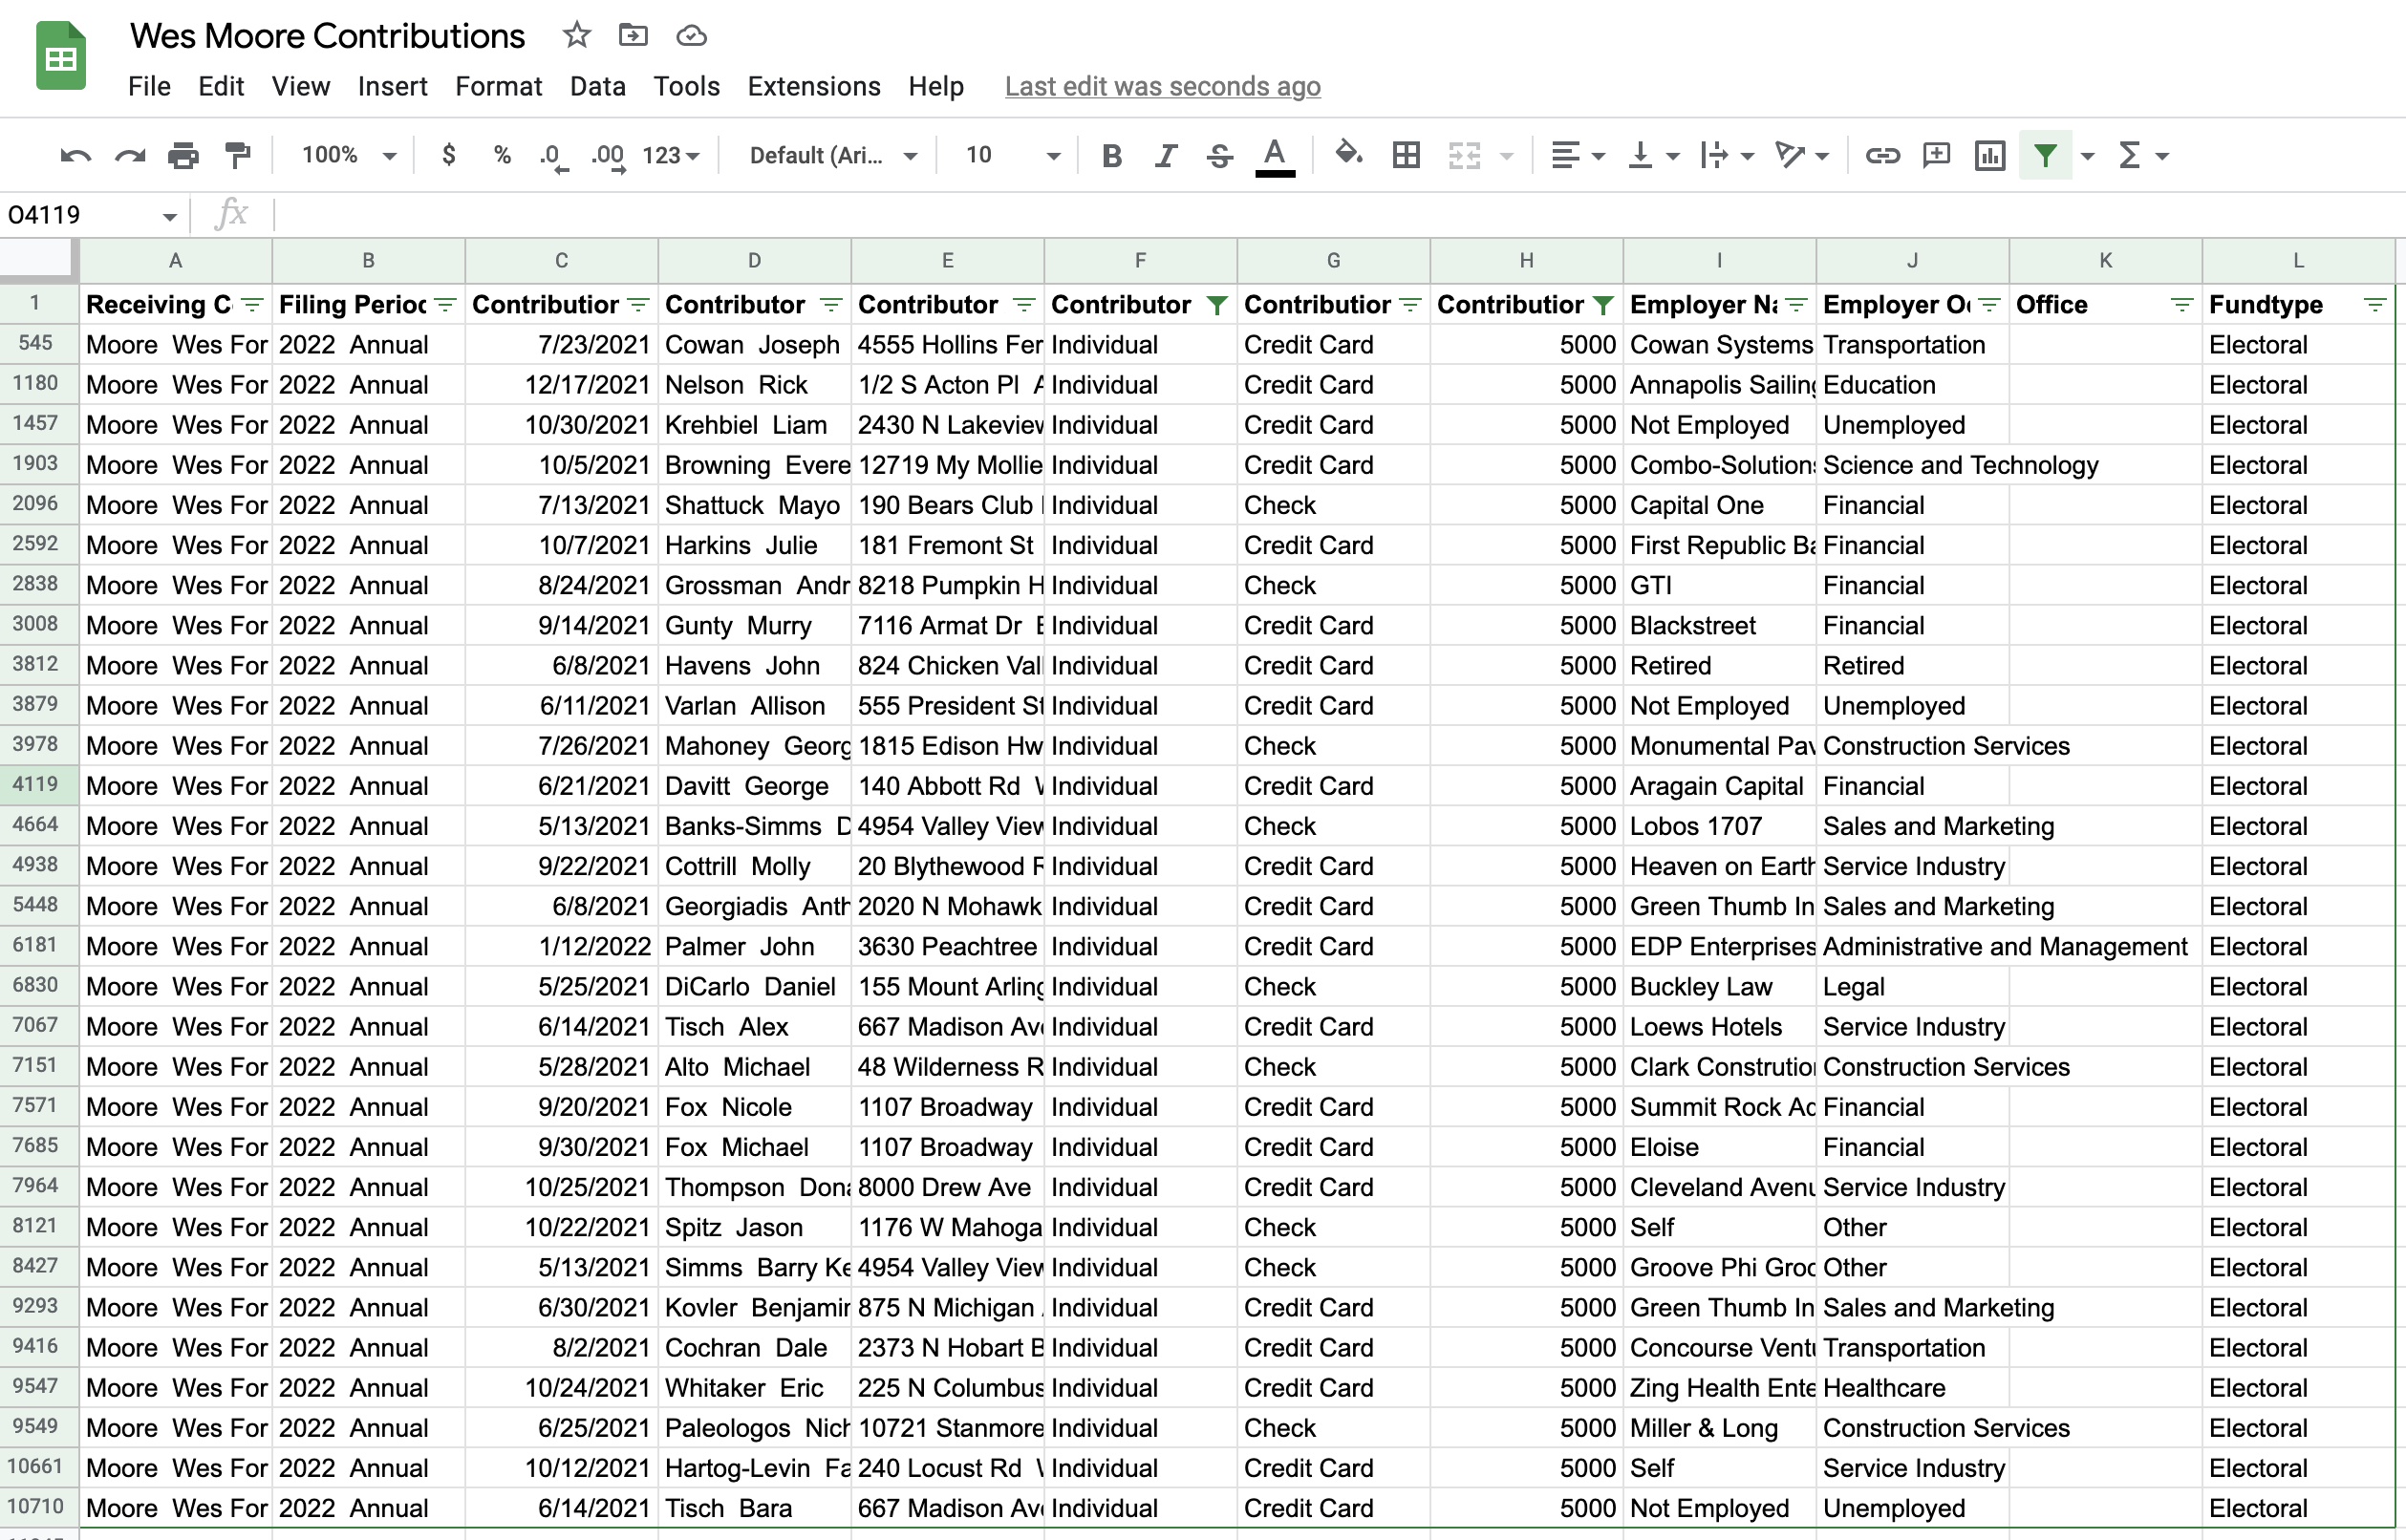
\includegraphics{./images/sheets-filter-sort-twofilters.png}

\hypertarget{different-kinds-of-filters}{%
\subsubsection*{Different kinds of
filters}\label{different-kinds-of-filters}}
\addcontentsline{toc}{subsubsection}{Different kinds of filters}

There are several options under the filter drop-down menu under ``Filter
by condition'', and you also can type values into a search box to try
and filter that way (the latter option is best for text columns). There
also is a ``Filter by color'' option. My opinion: don't do this.

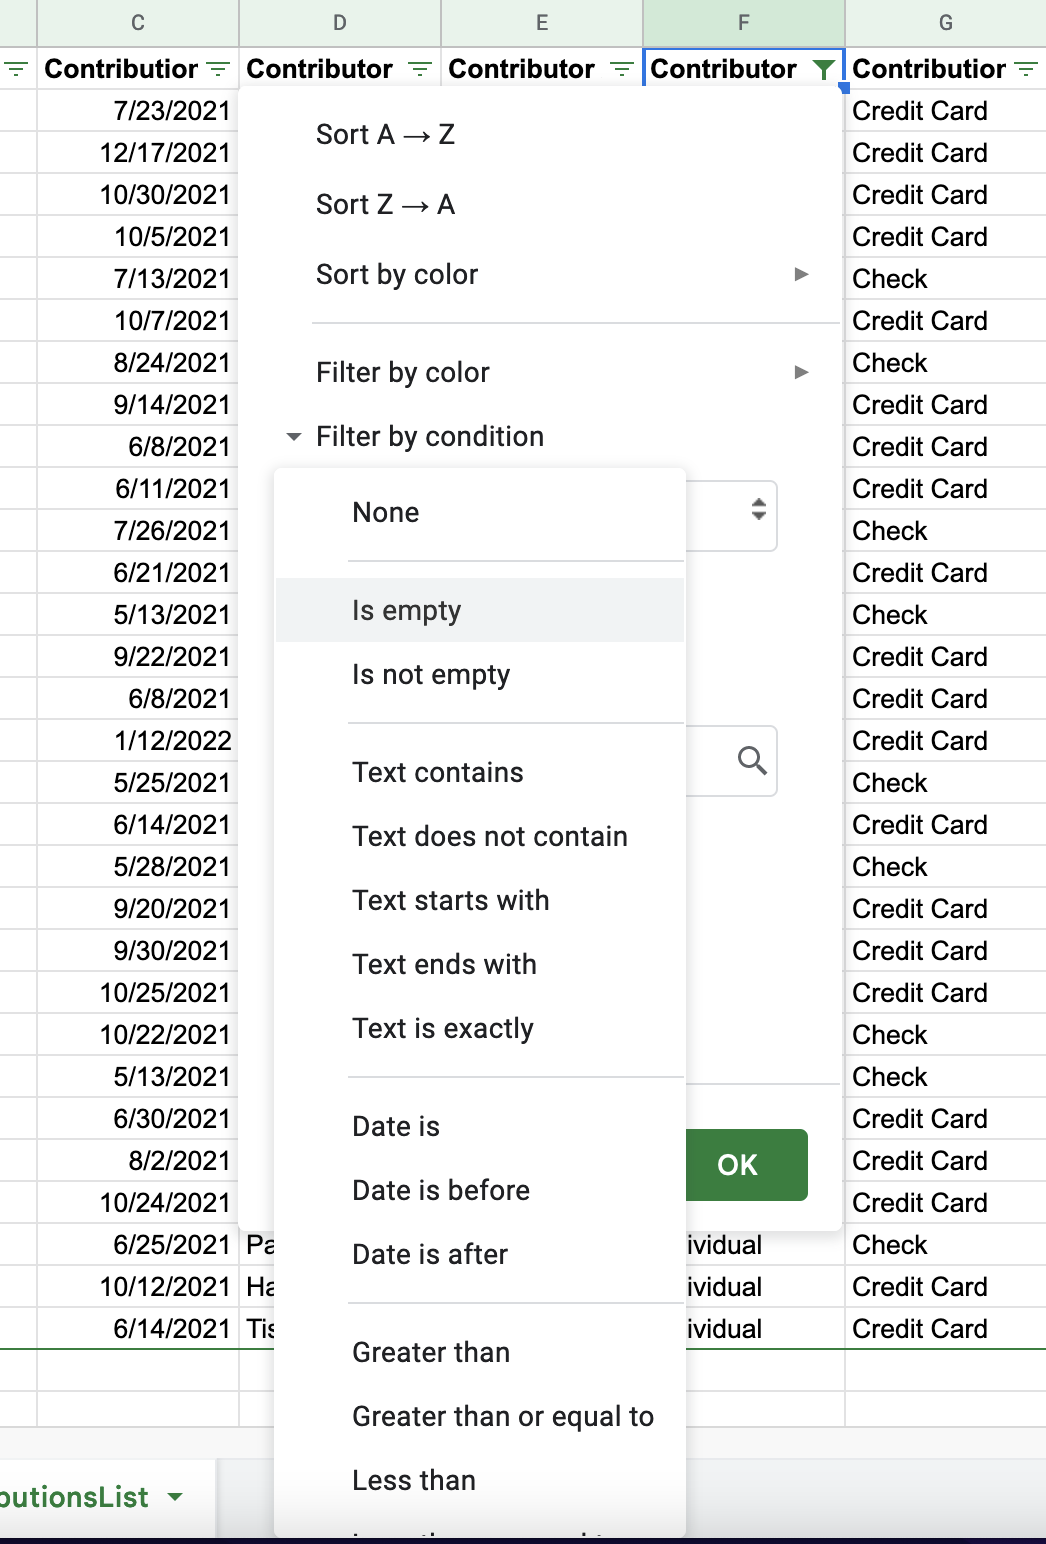
\includegraphics[width=0.3\textwidth,height=\textheight]{./images/sheets-filter-sort-filter-options.png}
\#\# FAQ

\hypertarget{how-do-i-turn-off-all-of-my-filters}{%
\subsection*{How do I turn off all of my
filters}\label{how-do-i-turn-off-all-of-my-filters}}
\addcontentsline{toc}{subsection}{How do I turn off all of my filters}

In the data tab, chose ``Remove filter'' to remove all of the filters.

\hypertarget{where-is-the-button-to-filter-columns}{%
\subsection*{\texorpdfstring{Where is the button to filter
\emph{columns}?}{Where is the button to filter columns?}}\label{where-is-the-button-to-filter-columns}}
\addcontentsline{toc}{subsection}{Where is the button to filter
\emph{columns}?}

Sometimes you don't want to see all of your columns -- there are too
many and they're getting confusing. There is no column filter in Sheets
or Excel (You'll see how to filter, or ``Select'', columns from a
dataset in R later.)

Instead, you can hide the columns you don't want to see. When columns
and rows are hidden, they generally won't copy to a new sheet.

\bookmarksetup{startatroot}

\hypertarget{xl-formulas}{%
\chapter{Formulas in Google Sheets}\label{xl-formulas}}

The quick review of math in Google Sheets uses the City of Phoenix's
budgeted spending for the 2018 fiscal year, compared with previous
years.

Make a copy of the
\href{https://docs.google.com/spreadsheets/d/1NGFHiJzvSsdB2wT7AehdSCjGrrwrOS1_rLk5FEaz7a8/edit?usp=sharing}{data
file} to follow along

You should get into the habit of creating unique identifiers, checking
your corners and looking for documentation before you ever start working
with a spreadsheet. These habits were covered in
\href{replication.html}{Data journalism in the age of replication} and
on \href{xl-refresher.html}{a Google Sheets refresher}.

\hypertarget{formulas-in-spreadsheets}{%
\section{Formulas in spreadsheets}\label{formulas-in-spreadsheets}}

Whether you use Google sheets or Excel, remember that every formula
begins with the equals sign \textbf{(=)}. Rather than the values you
want to work with in the formula, you'll use \emph{references} to other
cells in the sheet.

The easiest formulas are simple arithmetic: adding, subtracting,
multiplying and dividing two or more cells. You'll just use simple
operators to do this:

\begin{longtable}[]{@{}lll@{}}
\toprule()
operator & symbol & example \\
\midrule()
\endhead
addition & + & =A2+B2 \\
subtraction & - & =A2-B2 \\
multiplication & * & =A2*B2 \\
division & / & =A2/B2 \\
\bottomrule()
\end{longtable}

Here's what a spreadsheet looks like while editing some simple
arithmetic:

\begin{figure}

{\centering 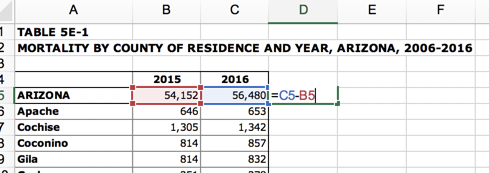
\includegraphics{./images/xl_mathreview_00.png}

}

\caption{formula}

\end{figure}

The other kind of formula is a \emph{function}. A function is a command
that has a name, and requires \emph{arguments} -- usually the cell
addresses or the range of addresses that it will act on. Every
programming language has functions built in and many have extensions, or
packages or libraries, that add even more as users find things they want
to do more efficiently. You begin using a function the same way you
begin a formula -- with an = sign. Here are three common functions that
create summary statistics for the numbers contained in a \emph{range} of
addresses. A range is a set of cells defined by its corner cell address:
the top left through the bottom right.

You'll usually use them on a single column at a time.

\begin{longtable}[]{@{}
  >{\raggedright\arraybackslash}p{(\columnwidth - 2\tabcolsep) * \real{0.3243}}
  >{\raggedright\arraybackslash}p{(\columnwidth - 2\tabcolsep) * \real{0.6757}}@{}}
\toprule()
\begin{minipage}[b]{\linewidth}\raggedright
Formula
\end{minipage} & \begin{minipage}[b]{\linewidth}\raggedright
What it does
\end{minipage} \\
\midrule()
\endhead
=SUM(start:finish) & Adds up the numbers between \texttt{start} and
\texttt{finish} \\
=AVERAGE(start:finish) & Computes the mean of the numbers \\
=MEDIAN(start:finish) & Derives the median of the numbers \\
\bottomrule()
\end{longtable}

\ldots where ``start'' means the first cell you want to include, and
finish means the last cell. Use the cell address of the first number you
want to include , a colon, then the cell address of the last number you
want to include. You can also select them while you're editing the
formula.

Here's an example of adding up all of the rows in a list by county:

\begin{figure}

{\centering 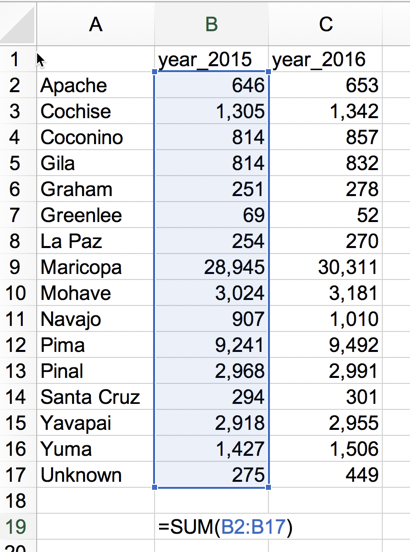
\includegraphics{./images/xl_mathreview_00A.png}

}

\caption{formula}

\end{figure}

\hypertarget{common-spreadsheet-arithmetic}{%
\section{Common spreadsheet
arithmetic}\label{common-spreadsheet-arithmetic}}

The budget document shows three years' of data: The actual spending in
the fiscal year that ended in 2016; the spending that was estimated for
the end of fiscal year 2017; and the proposed spending for fiscal year
2018. The first page of the document shows these amounts for broad
spending categories.

You may want to widen the columns and format the numbers before you
start:

\includegraphics[width=1\textwidth,height=\textheight]{./images/xl_mathreview_01.gif}

\hypertarget{check-the-governments-math-with-sum}{%
\subsection{Check the government's math with
SUM}\label{check-the-governments-math-with-sum}}

Our first job is to make sure the government has provided us data that
adds up. To do that, we'll SUM all of the departments' spending.

To add up the numbers from 2016, enter the following formula in cell
C11, just below the number provided by the government:

\begin{verbatim}
  =SUM(C2:C8)
  and hit the enter key
\end{verbatim}

Copy that formula to the right. Notice how the formula changes the
addresses that it is using as you move to the right -- it's adjusted
them to refer to the current column.

\includegraphics[width=1\textwidth,height=\textheight]{./images/xl_mathreview_02.gif}

What's wrong? The numbers for the budget 2018 don't add up. (Hint: look
at the page called ``notes'' for an explanation.)

\hypertarget{change-in-spending}{%
\subsection{Change in spending}\label{change-in-spending}}

The increase or decrease in projected spending from 2017 to 2018 is just
the difference between the two values, beginning in cell F3

\begin{verbatim}
  new-old, or  =E2-D2
\end{verbatim}

When you copy it down, note how the references to each row also
adjusted. In line 3, it's E3-D3, and so on. Excel and other spreadsheets
assume that, most of the time, you want these kinds of adjustments to be
made.

\includegraphics[width=1\textwidth,height=\textheight]{./images/xl_mathreview_03.gif}

\hypertarget{percent-change}{%
\subsection{Percent change}\label{percent-change}}

We can't tell the \emph{rate} of growth for each department until we
calculate the percent change from one year to another. Now that we
already have the change, the percent change is easy. The formula is:

\begin{verbatim}
  ( new - old ) / old

  .. or just scream "NOO"
\end{verbatim}

The new-old is already in column F, so all that's left is to divide
again. In grade school, you also had to move the decimal place over two
spots, since the concept of percent change is ``out of 100''. Excel
formats will do that for you.

Remember, it's always (new-old)/old , \textbf{NOT} the big one minus the
little one. Doing it correctly, the answer could be negative, meaning
the value fell.

\begin{figure}

{\centering 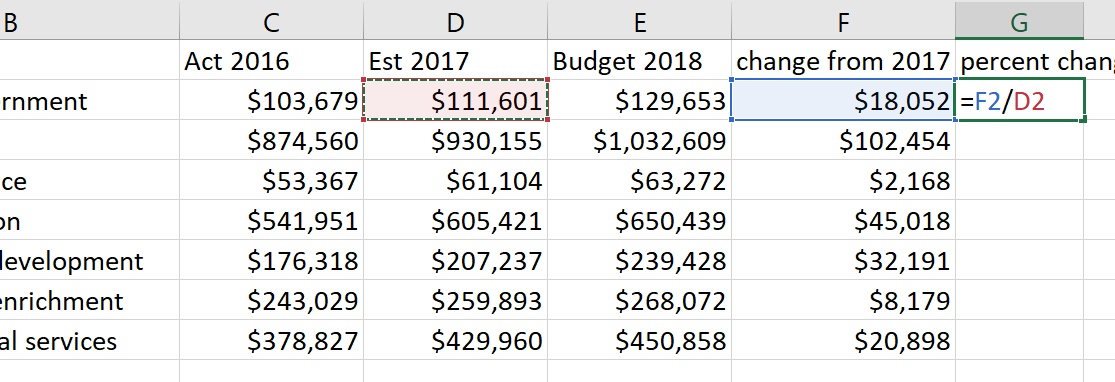
\includegraphics[width=1\textwidth,height=\textheight]{./images/xl_mathreview_04.png}

}

\caption{``\% change''}

\end{figure}

When you're done, you can format the answer as a percentage to get it
into whole numbers.

Until you get used to it, there's no harm in doing these calculations
step by step. Excel won't complain if you have extra columns. You can
always hide them.

It's also worth comparing the picture you get by looking at raw numbers
vs.~percentages. In our case, the budget for public safety is expected
to rise by a whopping \$102 million, but it's a smaller percentage
increase than other, smaller departments.

\hypertarget{parts-of-a-whole-percent-of-total}{%
\subsection{Parts of a whole: percent of
total}\label{parts-of-a-whole-percent-of-total}}

We'd also like to know what portion of the total spending is eaten up by
each department. To do that, we need the percent of total.

In our case, let's use the total that the government gave us. In
practice, you'd have to decide what to do if your figures didn't match
those provided by officials. You can't assume that the total is wrong --
you could be missing a category, or there could be a mistake in one of
the line items.

The formula for percent of total is:

\begin{verbatim}
  category / total
\end{verbatim}

Again, Excel will multiply by 100, or move the decimal place over for
you once you format.

But you have a problem: You either have to type in each row, or you get
something like this if you try to copy:

\begin{figure}

{\centering 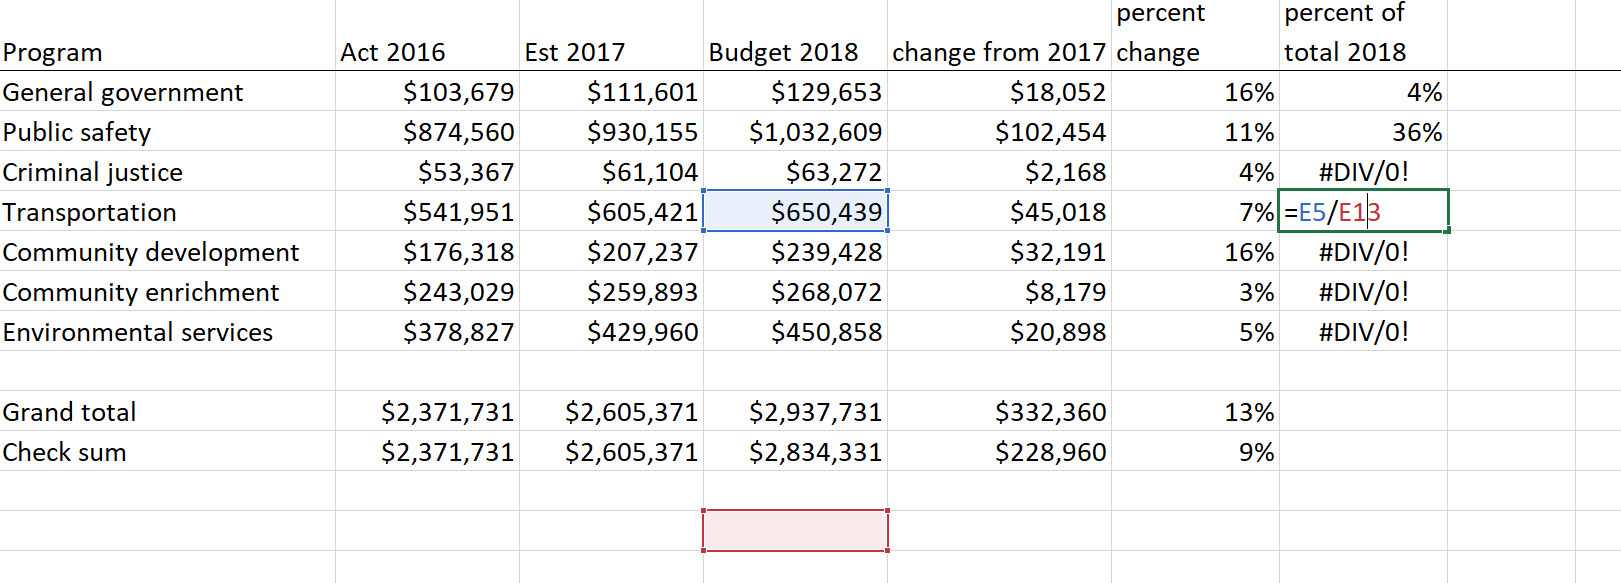
\includegraphics[width=1\textwidth,height=\textheight]{./images/xl_mathreview_05.png}

}

\caption{Wrong way}

\end{figure}

Excel has done its magic, adjusting the location of both the numerator
and the denominator when you copied. You don't have to type in each
formula one by one, though. Instead, you'll use anchors, known in
spreadsheets as ``absolute references''. Think of a dollar sign as an
anchor or stickpin, holding down the location of part of your formula.
If you put the stickpin before the letter in the formula, it holds the
column in place. If you put it before the number, it holds the row in
place. If you put it in both places, it holds the cell in place.

So our new formula for the percent of total is:

\begin{figure}

{\centering 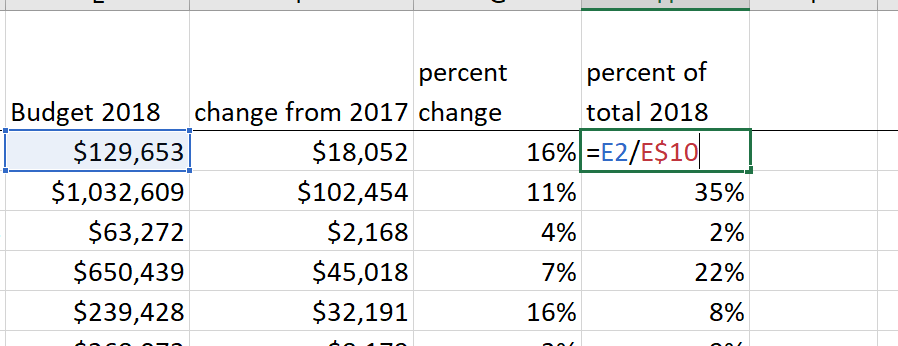
\includegraphics[width=1\textwidth,height=\textheight]{./images/xl_mathreview_06.png}

}

\caption{E2/E\$10}

\end{figure}

\hypertarget{while-were-at-it-two-kinds-of-averages}{%
\section{While we're at it: two kinds of
averages}\label{while-were-at-it-two-kinds-of-averages}}

Although it doesn't make a lot of sense in this context, we'll go ahead
and calculate the \emph{average} or \emph{mean} size of each department,
and then calculate the \emph{median} size.

\textbf{Simple average, or mean}

A simple average, also known as the mean, is skewed toward very high or
very low values. Its formula is

\begin{verbatim}
    sum of pieces / # of pieces that were summed
\end{verbatim}

But in Excel, all we need is the word AVERAGE:

\begin{verbatim}
    =AVERAGE(C2:C9)
\end{verbatim}

\textbf{Median}

In Excel, you can get the median of a list of numbers by just using the
formula, MEDIAN()

\begin{verbatim}
  = MEDIAN(C2:C9)
\end{verbatim}

\hypertarget{the-final-spreadsheet}{%
\section{The final spreadsheet}\label{the-final-spreadsheet}}

\begin{figure}

{\centering 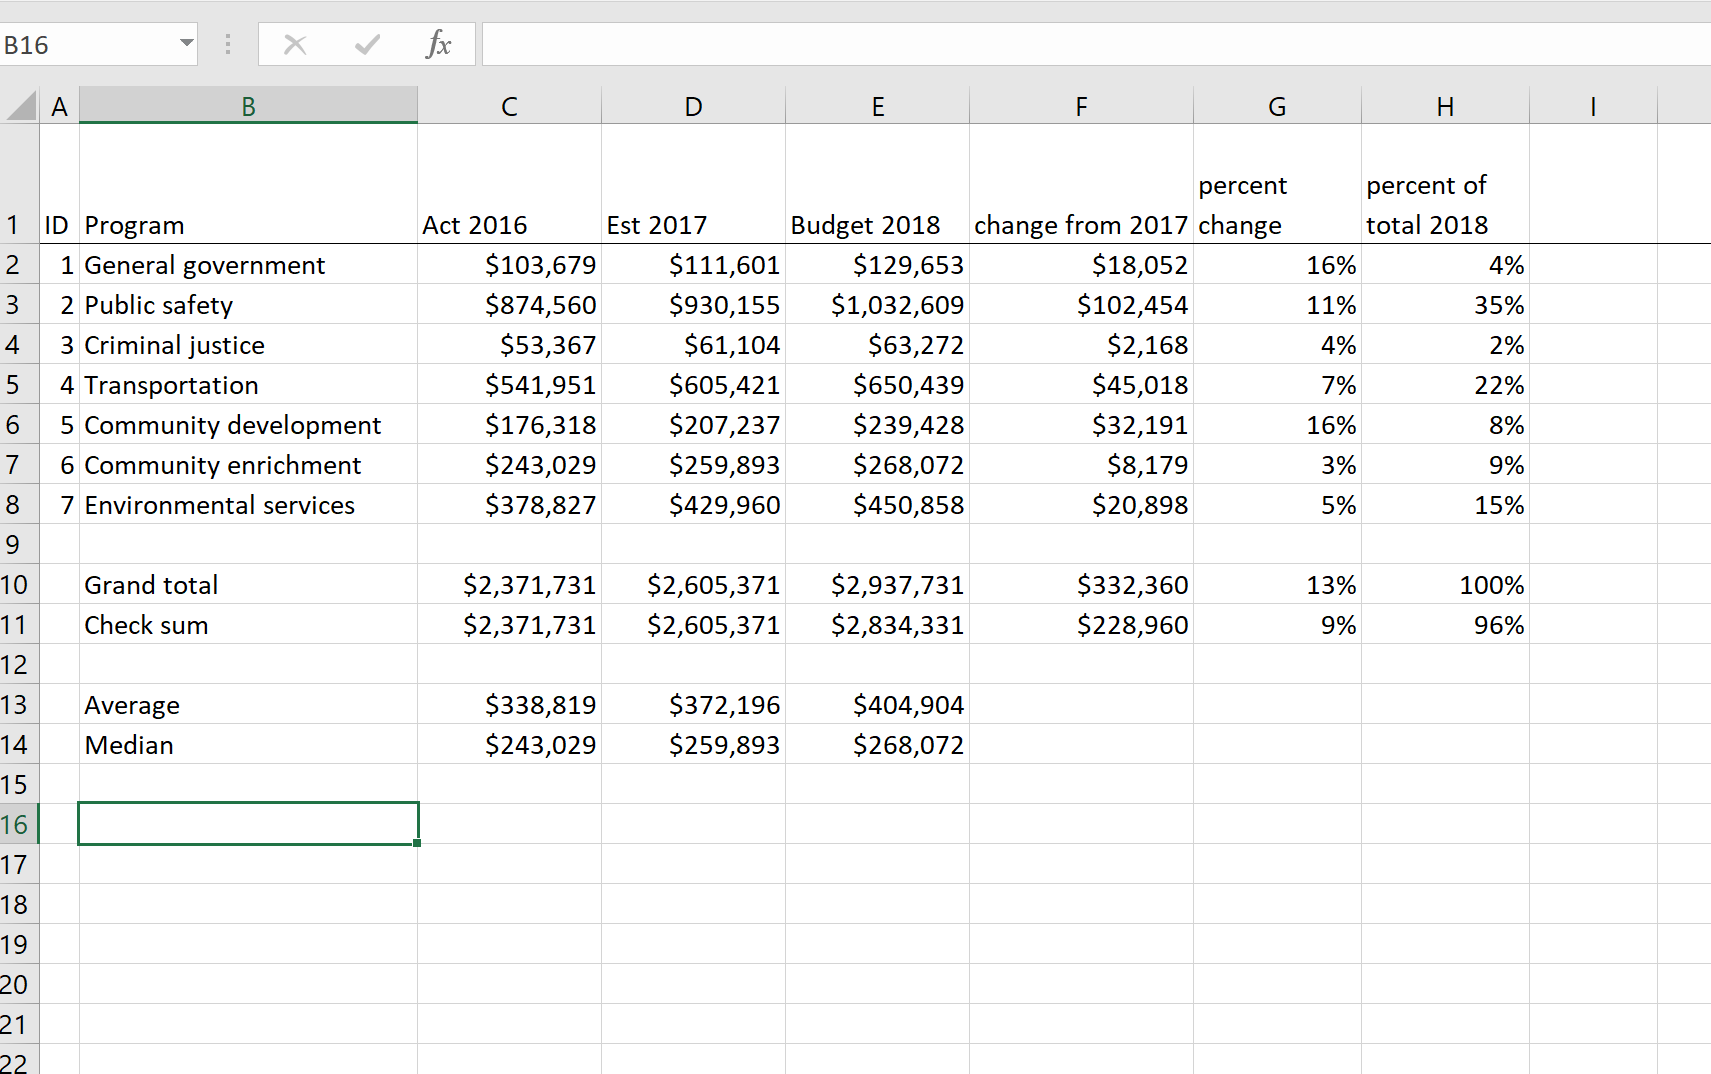
\includegraphics[width=1\textwidth,height=\textheight]{./images/xl_mathreview_07.png}

}

\caption{final worksheet}

\end{figure}

Doing simple calclutions like this on data that is provided to you by
the government lets you ask better questions when you get an interview,
and may even convince officials to talk with you. There's a big
difference between asking them to tell you what the budget numbers are,
and asking them to explain specific results!

\hypertarget{faqs}{%
\section{FAQs}\label{faqs}}

\hypertarget{sheets-wont-let-me-copy-my-formula}{%
\subsubsection*{Sheets won't let me copy my
formula}\label{sheets-wont-let-me-copy-my-formula}}
\addcontentsline{toc}{subsubsection}{Sheets won't let me copy my
formula}

Make sure your formula is locked in by either hitting ``Enter'' or
``Escape''. This is a common problem if you're in the habit of
double-clicking instead of selecting a cell. There are a lot things you
can't do while Excel thinks you're still entering information.

\hypertarget{should-i-use-average-or-median}{%
\subsubsection*{Should I use average or
median?}\label{should-i-use-average-or-median}}
\addcontentsline{toc}{subsubsection}{Should I use average or median?}

It depends. Averages are easier to explain but can be misleading.
Usually, if they're very different, median will be a better
representation of the typical person, city or department. Averages in
these cases are more like totals.

\hypertarget{my-percents-are-small-numbers-with-decimal-points}{%
\subsubsection*{My percents are small numbers with decimal
points}\label{my-percents-are-small-numbers-with-decimal-points}}
\addcontentsline{toc}{subsubsection}{My percents are small numbers with
decimal points}

Use the format as a \% button to move the decimal point over two places
and insert the percentage symbol.

\bookmarksetup{startatroot}

\hypertarget{xl-practice-noc}{%
\chapter{Practice exercise}\label{xl-practice-noc}}

This exercise helps you understand the difference between filtering and
grouping, or, in Excel terms, filtering and pivot tables. In general,
you'll use filtering to look up the details of cases based on a
criteria. These are the stories. You'll use pivot tables to create
aggregated data -- count, sum, average, and the like.

In the real world, reporters move back and forth between these two
techniques. They'll go back and filter for cases once they find
something interesting in the aggregation, and will create sums and
counts if they think they see a pattern in the cases.

That's pretty abstract concept -- it will become more concrete as you go
through the motions of this exercise.

\hypertarget{data-source}{%
\section{Data source}\label{data-source}}

\href{https://cronkitedata.s3.us-west-1.amazonaws.com/xlfiles/phx_claims_flagged.xlsx}{Data
download}

\href{https://www.phoenix.gov/financesite/Documents/City\%20of\%20Phoenix\%20Claim\%20Form\%20\%28REVISED\%206-7-21\%29.pdf}{City
link to Notice of claims form and instructions to claimants}

\href{https://docs.google.com/document/d/1j-vIiuysefqOrDAN-pIR5NqCq8mKqTBmQKcuhRLXy0o/edit?usp=sharing}{Backgrounder
on the data from Helen Wieffering}

This dataset includes all ``Notice of Claims'' against the city of
Phoenix between 2010 and 2020. These claims refer to damages that people
say they suffered because of a problem in the government ranging from
slip-and-fall in a city building to use of force by police. It was
obtained by Helen Wieffering just after the end of the 2020 fiscal year,
so many of the claims from that year will be unresolved. Although the
names of the claimants are public record, they were not included in the
data compiled here. Also missing is the court case number of any cases
that went to court.

Make sure to look at the ``data\_dictionary'' sheet for the definitions
of each column before you start.

In this tutorial, I'm providing the equivalent of a data diary for you
-- if you follow these instructions, you should come up with the same
answers I did. You should keep your own diary alongside your work.

\hypertarget{sort-filter}{%
\section{Sort / filter}\label{sort-filter}}

I almost always go into the Excel preferences, and under ``Tables \&
Filters'' turn off the check that says ``Use table names in formulas''.
Sometimes it sticks, sometimes it doesn't. Have no idea why.

Arrange (sort) the claims using the ID column which is called
``orig\_order''.

\begin{enumerate}
\def\labelenumi{\arabic{enumi}.}
\item
  What is the orig\_order (id) value of the largest PAID claim in the
  database (combined personal injury and property) ?
\item
  What department and cause were associated with that payment?
\item
  How long did it take to resolve it?
\item
  Describe the most recent claim made against the police related to law
  enforcement activities, regardless of whether it's been resolved.
\item
  Filter for pd\_total of greater than zero, and the type called
  ``Shootings''. Look at the lower left corner and record how many
  claims against the city for shootings were paid any money?
\item
  Find one other thing that you might want to research further that
  could make an interesting one-off story. These are distinct events
  that you'd like to know more about, not trends or patterns. This
  requires no calculation, just your news judgment.
\end{enumerate}

\hypertarget{pivot-table-motivation}{%
\section{Pivot table motivation}\label{pivot-table-motivation}}

Here are some questions you have about each department in the city:

\begin{itemize}
\tightlist
\item
  What was the highest and lowest payout they made?
\item
  How many claims were made, and how many were paid out?
\item
  What was the total amount paid and the average per claim?
\end{itemize}

\hypertarget{using-filters-to-answer-big-questions}{%
\subsection{Using filters to answer big
questions}\label{using-filters-to-answer-big-questions}}

Here's one way to do it, using the filters:

\begin{enumerate}
\def\labelenumi{\arabic{enumi}.}
\tightlist
\item
  Remove all of your filter.
\item
  Filter by department. We'll start with Aviation, the first one on the
  list.
\item
  Select the entire table, including the headings. Copy it to a new
  sheet. Don't be surprised if you miss the headings or some of the
  columns the first couple of times through and have to do it again.\\
\item
  Rename the new sheet ``Aviation'' by double-clicking on its tab.
\item
  Make sure you're in the top left corner of the screen (use CTL-HOME
  key if you're on a real keyboard, CTL-UP and CTL-Left if you're not.)
  Freeze the column headings so you can scroll to the bottom and still
  see what you're looking at (under View, Freeze top Row)
\item
  Note the number of rows that were copied and subtract one. Record that
  as the number of claims made.
\item
  Make sure you start from the top of the sheet, and filter out
  ``Unresolved'' claims by un-selecting it. Don't touch anything before
  you note the number of records found at the bottom left (it should be
  11852 in this case). That's the number of resolved claims. Now filter
  on the same column, and uncheck ``No payment'' and note the number of
  claims. It should be 5718.
\item
  Go to the bottom of the worksheet. Skip a row, and sum the column.
  Repeat that, replacing =sum() with =max(), =min() , =average().
\item
  Write down all of your answers on a piece of paper.
\end{enumerate}

Don't be surprised if you do this wrong a few times, and you have to do
it over. But now you have the answer for the Aviation department.

Try to imagine what you'd do if you wanted to know the average and
minimum payout of just those that were settled .

\hypertarget{rinse-repeat}{%
\section{Rinse, repeat}\label{rinse-repeat}}

Now repeat that entire process with at least two other departments that
interest you.

\hypertarget{pivot-table}{%
\section{Pivot table}\label{pivot-table}}

At this point, you should be thoroughly sick of having to do things over
and over. The purpose of the pivot table is to let you compute these
aggregate, or summary, statistics all at once for each category or set
of categories. It can compute average, minimum , maximum and sum of
values, and it can count the number of rows for any column. (In Excel
they're always the same. That's not always true of all programs
depending on how they handle missing information.)

\hypertarget{create-the-pivot-table}{%
\subsection{Create the pivot table}\label{create-the-pivot-table}}

1, Create an empty pivot table from the data table.

\begin{enumerate}
\def\labelenumi{\arabic{enumi}.}
\setcounter{enumi}{1}
\item
  Look for the ``Options'' tab toward the top left, and turn off
  ``Generate GetPivotData''. In the same tab, under ``Options'', set
  error values to ``N/A'', and set Empty cells to zero (meaning there
  was nothing in that category.)
\item
  Drag ``Department'' to the row area
\item
  Drag the type\_case to the filter area
\item
  Drag the ``department'' to the Values area and make sure it says
  ``Count of Department''.
\item
  Drag the pd\_total to the Values area, and make sure it says ``Sum of
  pd\_total''. If it doesn't, change the pivot table calculation to
  ``Sum''. Repeat that three times, with ``average'', ``min'' and
  ``max''.
\end{enumerate}

Try playing with the placement of items in the pivot table to get an
intuition for what they do. You can drag a column into the ``Filter''
area so that you can pick out just some of the cases for analysis. It
works the same way as the filter in the original sheet.

\hypertarget{practice-questions}{%
\subsection{Practice questions}\label{practice-questions}}

Now answer the following questions:

\begin{enumerate}
\def\labelenumi{\arabic{enumi}.}
\item
  What department had the most claims made against them from FY 2015-16
  to through 2019-20?
\item
  How much did the city pay in that time because of complaints against
  Streets. Did any department pay more?
\item
  On average, how much did the city pay vs.~the amount that was
  requested? Include only those complaints that have been resolved --
  not those that are still underway or have been reopened.
\end{enumerate}

\bookmarksetup{startatroot}

\hypertarget{ethics-in-data-journalism}{%
\chapter{Ethics in data journalism}\label{ethics-in-data-journalism}}

\href{https://source.opennews.org/articles/public-info-doesnt-always-want-be-free/}{This
originally appeared on Open News in March 2013}.

In 2009, a senior web editor asked me and another developer a question:
could our development group build a new news application for
Tampabay.com that displayed a gallery of mug shots? Stories about goofy
crimes with strange mug shots were popular with readers. The vision, on
the part of management, was a website that would display the mugshots
collected every day from publicly available websites by two
editors---well paid, professional editors with other responsibilities.

Newsrooms are many things. Alive. Filled with energy. Fueled by stress,
coffee and profanity. But they are also idea factories. Day after day,
ideas come from everywhere. From reporters on the beat. From editors
reading random things. From who knows where. Some of them are brilliant.
Some would never work. Most need more people and time than are
available. And some are dumber than anyone cares to admit.

We thought this idea was nuts. Why would we pay someone, let alone an
editor, to fetch mug shots from the Internet? Couldn't we do that with a
scraper?

If only this were the most complex question we would face.

Because given enough time and enough creativity, scraping a mug shot
website is easy. You need to recognize a pattern, parse some HTML and
gather the pieces you need. At least that's how it should work. Police
agencies that put mugs online usually buy software from a vendor.
Apparently, those vendors enjoy making horrific, non-standard,
broken-in-interesting-and-unique-ways HTML. You'll swear. A lot. But
you'll grind it out. And that's part of the fun. Scraping isn't any fun
with clean, semantic, valid HTML. And scraping mug shot websites, by
that definition, is tons of fun.

The complexity comes when you realize the data you are dealing with
represent real people's lives.

\hypertarget{problems}{%
\section{Problems}\label{problems}}

The first problem we faced, long before we actually had data, was that
data has a life of its own. Because we were going to put this
information in front of a big audience, Google was going to find it.
That meant if we used our normal open door policy for the Googlebot,
someone's mug shot was going to be the first record in Google for their
name, most likely. It would show up first because most people dont
actively cultivate their name on the web for visibility in Google. It
would show up first because we know how SEO works and they dont. It
would show up first because our site would have more traffic than their
site, and so Google would rank us higher.

And that record in Google would exist as long as the URL did. Longer
when you consider the cached versions Google keeps.

That was a problem because here are the things we could not know:

\begin{itemize}
\tightlist
\item
  Was this person wrongly arrested?
\item
  Was this person innocent?
\item
  Were the charges dropped against this person?
\item
  Did this person lie about any of their information?
\end{itemize}

\hypertarget{the-googlebot}{%
\section{The Googlebot}\label{the-googlebot}}

So it turned out to be very important to know the Googlebot. It's your
friend \ldots{} until it isn't. We went to our bosses and said words
that no one had said to them before: we did not want Google to index
these pages. In a news organization, the page view is the coin of the
realm. It is --- unfortunately --- how many things are evaluated when
the bosses ask if it was successful or not. So, with that in mind,
Google is your friend. Google brings you traffic. Indeed, Google is your
single largest referrer of traffic at a news organization, so you want
to throw the doors open and make friends with the Googlebot.

But here we were, saying Google wasn't our friend and that we needed to
keep the Googlebot out. And, thankfully, our bosses listened to our
argument. They too didn't want to be the first result in Google for
someone.

So, to make sure we were telling the Googlebot no, we used three lines
of defense. We told it no in robots.txt and on individual pages as a
meta tag, and we put the most interesting bits of data into a simple
JavaScript wrapper that made it hard on the bot if the first two things
failed.

The second solution had ramifications beyond the Googlebot. We decided
that we were not trying to make a complete copy of the public record.
That existed already. If you wanted to look at the actual public
records, the sheriff's offices in the area had websites and they were
the official keeper of the record. We were making browsing those images
easy, but we were not the public record.

That freedom had two consequences: it meant our scrapers could, at a
certain point and given a number of failures, just give up on getting a
mug. Data entered by humans will be flawed. There will be mistakes.
Because of that, our code would have to try and deal with that. Well,
there's an infinite number of ways people can mess things up, so we
decided that since we were not going to be an exact copy of the public
record, we could deal with the most common failures and dump the rest.
During testing, we were getting well over 98\% of mugs without having to
spend our lives coding for every possible variation of typo.

The second consequence of the decision actually came from the newspapers
lawyers. They asked a question that dumbfounded us: How long are you
keeping mugs? We never thought about it. Storage was cheap. We just
assumed we'd keep them all. But, why should we do that? If we're not a
copy of the public record, we dont have to keep them. And, since we
didnt know the result of each case, keeping them was really kind of
pointless.

So, we asked around: How long does a misdemeanor case take to reach a
judgement? The answer we got from various sources was about 60 days.
From arrest to adjudication, it took about two months. So, at the 60 day
mark, we deleted the data. We had no way of knowing if someone was
guilty or innocent, so all of them had to go. We even called the script
The Reaper.

We'd later learn that the practical impacts of this were nil. People
looked at the day's mugs and moved on. The amount of traffic a mug got
after the day of arrest was nearly zero.

\hypertarget{data-lifetimes}{%
\section{Data Lifetimes}\label{data-lifetimes}}

The life of your data matters. You have to ask yourself, Is it useful
forever? Does it become harmful after a set time? We had to confront the
real impact of deleting mugs after 60 days. People share them,
potentially lengthening their lifetime long after they've fallen off the
homepage. Delete them and that URL goes away.

We couldn't stop people from sharing links on social media---and indeed
probably didn't want to stop them from doing it. Heck, we did it while
we were building it. We kept IMing URLs to each other. And that's how we
realized we had a problem. All our work to minimize the impact on
someone wrongly accused of a crime could be damaged by someone sharing a
link on Facebook or Twitter.

There's a difference between frictionless and unobstructed sharing and
some reasonable constraints.

We couldn't stop people from posting a mug on Facebook, but we didn't
have to make it easy and we didn't have to put that mug front and
center. So we blocked Facebook from using the mug as the thumbnail image
on a shared link. And, after 60 days, the URL to the mug will throw a
404 page not found error. Because it's gone.

We couldn't block Google from memorializing someone's arrest, only to
let it live on forever on Facebook.

\hypertarget{you-are-a-data-provider}{%
\section{You Are a Data Provider}\label{you-are-a-data-provider}}

The last problem didn't come until months later. And it came in the
middle of the night. Two months after we launched, my phone rang at 1
a.m. This is never a good thing. It was my fellow developer, Jeremy
Bowers, now with NPR, calling me from a hotel in Washington DC where he
was supposed to appear in a wedding the next day. Amazon, which we were
using for image hosting, was alerting him that our bandwidth bills had
tripled on that day. And our traffic hadn't changed.

What was going on?

After some digging, we found out that another developer had scraped our
site---because we were so much easier to scrape than the Sheriff's
office sites---and had built a game out of our data called Pick the
Perp. There were two problems with this: 1. The game was going viral on
Digg (when it was still a thing) and Reddit. It was getting huge
traffic. 2. That developer had hotlinked our images. He/she was serving
them from our S3 account, which meant we were bearing the costs. And
they were going up exponentially by the minute.

What we didn't realize when we launched, and what we figured out after
Pick the Perp, was that we had become data provider, in a sense. We had
done the hard work of getting the data out of a website and we put it
into neat, semantic, easily digestible HTML. If you were after a stream
of mugshots, why go through all the hassle of scraping four different
sheriff's office's horrible HTML when you could just come get ours
easily?

Whoever built Pick the Perp, at least at the time, chose to use our
site. But, in doing so, they also chose to hotlink images---use the URL
of our S3 bucket, which cost us money---instead of hosting the images
themselves.

That was a problem we hadn't considered. People hotlink images all the
time. And, until those images are deleted from our system, they'll stay
hotlinked somewhere.

Amazon's S3 has a system where you can attach a key to a file that
expires after X period of time. In other words, the URL to your image
only lasts 15 minutes, or an hour, or however long you decide, before it
breaks. It gives you fine grained control over how long someone can use
your image URL.

So at 3 a.m., after two hours of pulling our hair out, we figured out
how to sync our image keys with our cache refreshes. So every 15
minutes, a url to an image expired and Pick the Perp came crashing down.

While the Pick the Perp example is an easy one---it's never cool to
hotlink an image---it does raise an issue to consider. Because you are
thinking carefully about how to build your app the right way doesn't
mean someone else will. And it doesn't mean they won't just go take your
data from your site. So how could you deal with that? Make the data
available as a download? Create an API that uses your same ethical
constructs? Terms of service? All have pros and cons and are worth
talking about before going forward.

\hypertarget{ethical-data}{%
\section{Ethical Data}\label{ethical-data}}

We live in marvelous times. The web offers you no end of tools to make
things on the web, to put data from here on there, to make information
freely available. But, we're an optimistic lot. Developers want to
believe that their software is being used only for good. And most people
will use it for good. But, there are times where the data you're working
with makes people uncomfortable. Indeed, much of journalism is about
making people uncomfortable, publishing things that make people angry,
or expose people who don't want to be exposed.

What I want you to think about, before you write a line of code, is what
does it mean to put your data on the internet? What could happen, good
and bad? What should you do to be responsible about it?

Because it can have consequences.

On Dec.~23, the Journal News in New York published a map of every legal
gun permit holder in their home circulation county. It was a public
record. They put it into Google Fusion Tables and Google dutifully
geocoded the addresses. It was a short distance to publication from
there.

Within days, angry gun owners had besieged the newspaper with
complaints, saying the paper had given criminals directions to people's
houses where they'd find valuable guns to steal. They said the paper had
violated their privacy. One outraged gun owner assembled a list of the
paper's staff, including their home addresses, telephone numbers, email
addresses and other details. The paper hired armed security to stand
watch at the paper.

By February, the New York state legislature removed handgun permits from
the public record, citing the Journal News as the reason.

There's no end of arguments to be had about this, but the simple fact is
this: The reason people were angry was because you could click on a dot
on the map and see a name and an address. In Fusion Tables, removing
that info window would take two clicks.

Because you can put data on the web does not mean you should put data on
the web. And there's a difference between a record being ``public'' and
``in front of a large audience.''

So before you write the first line of code, ask these questions:

\begin{itemize}
\tightlist
\item
  This data is public, but is it widely available? And does making it
  widely available and easy to use change anything?
\item
  Should this data be searchable in a search engine?
\item
  Does this data expose information someone has a reasonable expectation
  that it would remain at least semi-private?
\item
  Does this data change over time?
\item
  Does this data expire?
\item
  What is my strategy to update or delete data?
\item
  How easy should it be to share this data on social media?
\item
  How should I deal with other people who want this data? API? Bulk
  download?
\end{itemize}

Your answers to these questions will guide how you build your app. And
hopefully, it'll guide you to better decisions about how to build an app
with ethics in mind.

\bookmarksetup{startatroot}

\hypertarget{public-records}{%
\chapter{Public records}\label{public-records}}

Public records are the lifeblood of investigative reporting. They carry
their own philosophical framework, in a manner of speaking.

\begin{itemize}
\tightlist
\item
  Sunlight is the best disinfectant. Corruption hides in the shadows.
\item
  You paid for it with your taxes. It should be yours (with exceptions).
\item
  Journalism with a capital J is about holding the powerful accountable
  for their actions.
\end{itemize}

Keeping those things in mind as you navigate public records is helpful.

\hypertarget{federal-law}{%
\section{Federal law}\label{federal-law}}

Your access to public records and public meetings is a matter of the
law. As a journalist, it is your job to know this law better than most
lawyers. Which law applies depends on which branch of government you are
asking. In addition to documents and other kinds of information, FOIA
also provides access to structured datasets of the kind we'll use in
this class.

The Federal Government is covered by the Freedom of Information Act, or
FOIA. FOIA is not a universal term. Do not use it if you are not talking
to a federal agency. FOIA is a beacon of openness to the world. FOIA is
deeply flawed and frustrating.

Why?

\begin{itemize}
\tightlist
\item
  There is no real timetable with FOIA. Requests can take months, even
  years.
\item
  As a journalist, you can ask that your request be expedited.
\item
  Guess what? That requires review. More delays.
\item
  Exemptions are broad. National security, personal privacy, often
  overused.
\item
  Denied? You can appeal. More delays.
\end{itemize}

The law was enacted in 1966, but it's still poorly understood by most
federal employees, if not outright flouted by political appointees.
Lawsuits are common.

Post 9/11, the Bush administration rolled back many agency rules. Obama
ordered a ``presumption of openness'' but followed it with some of the
most restrictive policies ever seen. The Trump Administration, similar
to the Obama administration, claims to be the most transparent
administration, but has steadily removed records from open access and
broadly denied access to records.

Result? FOIA is in trouble.

\href{https://www.spj.org/foi-guide-pros.asp}{SPJ is a good resource}.

\hypertarget{state-law}{%
\section{State law}\label{state-law}}

States are -- generally -- more open than the federal government. The
distance between the government and the governed is smaller. Some
states, like Florida and Texas, are very open. Others, like Virginia and
Pennsylvania, are not. Maryland is somewhere in the middle.

These laws generally give you license to view -- and obtain a copy of --
a record held by a state or local government agency.

What is a public record? Generally speaking, public records are
information stored on paper or in an electronic format held by a state
or local government agency, but each state has its own list of types of
records -- called ``exemptions'' -- that are not subject to disclosure.

If a record has both exempt and non-exempt information mixed in, most
states require an agency to disclose it after removing the exempt
information, a process called ``redaction.'' Agencies aren't required to
create a record in order to fill your request.

In some states but not all -- the public information law (or related
case law) explicitly dictates that extracting a slice of a database
doesn't constitute creation of a record. Most states can charge you a
reasonable fee for time spent retrieving or copying records, though many
have provisions to waive those fees for journalists. Every state law
operates on a different timeline. Some only require agencies respond in
a ``reasonable'' time, but others spell out exactly how fast an agency
must respond to you, and how fast they must turn over the record.

\href{https://www.rcfp.org/open-government-guide/}{The Reporters
Committee For Freedom of the Press} has a good resource for learning the
law in your state.

Please and thank you will get you more records than any lawyer or
well-written request. Be nice. Be polite. And be persistent. Following
up regularly to check on status of a request lets an agency know they
can't ignore you (and some will try). Hunting for records is like any
other kind of reporting -- you have to do research. You have to ask
questions. Ask them: What records do you keep? For how long?

When requesting data, you are going to scare the press office and you
are going to confuse the agency lawyer. Request to have their data
person on the phone.

A good source of info? Records retention schedules, often required by
law or administrative rule at an agency. Here's an example from
\href{https://www.courts.state.md.us/sites/default/files/import/circuit/pdfs/retentionschedule_2330.pdf}{Maryland's
Circuit Courts}.

\bookmarksetup{startatroot}

\hypertarget{using-github}{%
\chapter{Using GitHub}\label{using-github}}

GitHub is a platform for managing and storing files, data and code built
atop Git, a popular open source version control software. GitHub
accounts are free and it's
\href{https://docs.github.com/en/get-started/quickstart}{easy to get
started}. The one prerequisite is that you have
\href{https://docs.github.com/en/get-started/quickstart/set-up-git}{Git
installed on your local computer}. There are installers for Mac, Windows
and Linux.

\hypertarget{how-it-works}{%
\section{How It Works}\label{how-it-works}}

Version control is based on the ideas that you want to keep track of
changes you make to a collection of files and that multiple people can
work together without getting in each other's way or having to do things
in a set order. For individual users, it's great for making sure that
you always have your work.

GitHub users work in what are known as repositories on their local
computers and also \emph{push} changes to a remote repository located on
GitHub. That remote repository is key: if you lose your computer, you
can fetch a version of your files from GitHub. If you want to work with
someone else on the same files, you can each have a local copy, push
changes to GitHub and then pull each others' changes back to your local
computers.

So, like Microsoft Word's track changes but with a remote backup and
multiple editors.

\hypertarget{getting-started}{%
\section{Getting Started}\label{getting-started}}

After installing Git and signing up for a GitHub account,
\href{https://docs.github.com/en/desktop/installing-and-configuring-github-desktop}{download
and install GitHub Desktop}. It will have you sign into your GitHub
account and then you'll have access to any existing repositories. If you
don't have any, that's fine! You can
\href{https://docs.github.com/en/desktop/installing-and-configuring-github-desktop/overview/creating-your-first-repository-using-github-desktop}{make
one locally}.

GitHub has
\href{https://docs.github.com/en/desktop/contributing-and-collaborating-using-github-desktop}{good
documentation for working in the Desktop app}, and while the emphasis in
this book will be on using GitHub for version control, it also supports
recording issues (read: problems or questions) with your files,
contributing to projects that aren't yours and more.

\hypertarget{advanced-use}{%
\section{Advanced Use}\label{advanced-use}}

Although our focus is on the GitHub Desktop app, you can use Git and
GitHub from your computer's command line interface, and GitHub has a
purpose-built \href{https://docs.github.com/en/github-cli}{command line
client}, too. GitHub can also serve as a publishing platform for many
types of files, and entire websites are hosted on
\href{https://docs.github.com/en/pages}{GitHub Pages}.

\bookmarksetup{startatroot}

\hypertarget{r-basics}{%
\chapter{R Basics}\label{r-basics}}

\href{https://www.r-project.org/about.html}{R} is a programming
language, one specifically geared toward data analysis.

Like all programming languages, it has certain built-in functions.

There are many ways you can write and execute R code. The first, and
most basic, is the console, shown here as part of a software tool called
\href{https://www.rstudio.com/products/rstudio/}{RStudio (Desktop Open
Source Edition)} that we'll be using all semester.

\begin{figure}

{\centering 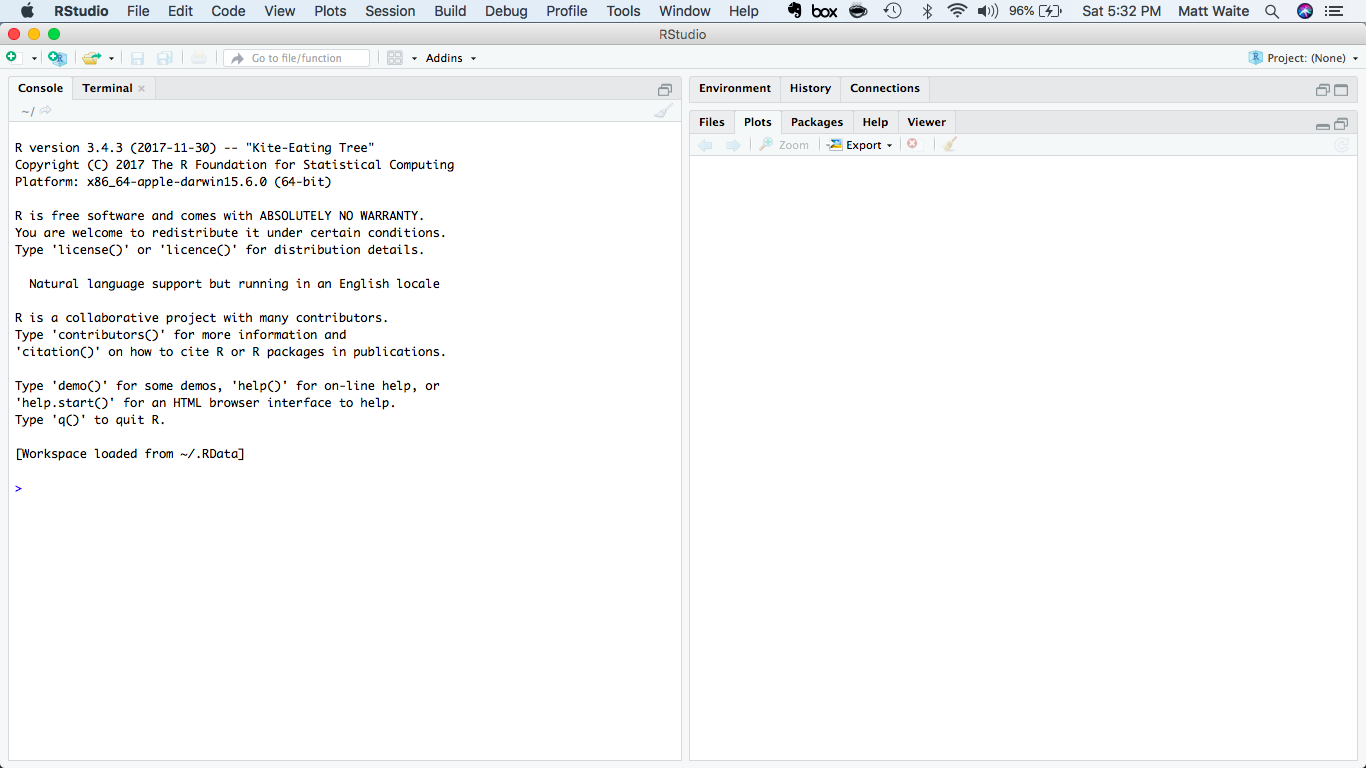
\includegraphics{./images/verybasics1.png}

}

\caption{ready}

\end{figure}

Think of the console like talking directly to the R language engine
that's busy working inside your computer. You use it send R commands,
making sure to use the only language it understands, which is R. The R
language engine processes those commands, and sends information back to
you.

Using the console is direct, but it has some drawbacks and some quirks
we'll get into later. Let's examine a basic example of how the console
works.

If you load up R Studio, type 2+2 into the console and hit enter it will
spit out the number 4, as displayed below.

\begin{Shaded}
\begin{Highlighting}[]
\DecValTok{2}\SpecialCharTok{+}\DecValTok{2}
\end{Highlighting}
\end{Shaded}

\begin{verbatim}
[1] 4
\end{verbatim}

It's not very complex, and you knew the answer before hand, but you get
the idea. With R, we can compute things.

We can also store things for later use under a specific name. In
programming languages, these are called \textbf{variables}. We can
assign things to variables using this left-facing arrow:
\texttt{\textless{}-}. The \texttt{\textless{}-} is a called an
\textbf{assignment operator}.

If you load up R studio and type this code in the console\ldots{}

\begin{Shaded}
\begin{Highlighting}[]
\NormalTok{number }\OtherTok{\textless{}{-}} \DecValTok{2}
\end{Highlighting}
\end{Shaded}

\ldots and then type this code, it will spit out the number 4, as show
below.

\begin{Shaded}
\begin{Highlighting}[]
\NormalTok{number }\SpecialCharTok{*}\NormalTok{ number}
\end{Highlighting}
\end{Shaded}

\begin{verbatim}
[1] 4
\end{verbatim}

We can have as many variables as we can name. We can even reuse them
(but be careful you know you're doing that or you'll introduce errors).

If you load up R studio and type this code in the console\ldots{}

\begin{Shaded}
\begin{Highlighting}[]
\NormalTok{firstnumber }\OtherTok{\textless{}{-}} \DecValTok{1}
\NormalTok{secondnumber }\OtherTok{\textless{}{-}} \DecValTok{2} 
\end{Highlighting}
\end{Shaded}

\ldots and then type this, it will split out the number 6, as shown
below.

\begin{Shaded}
\begin{Highlighting}[]
\NormalTok{(firstnumber }\SpecialCharTok{+}\NormalTok{ secondnumber) }\SpecialCharTok{*}\NormalTok{ secondnumber}
\end{Highlighting}
\end{Shaded}

\begin{verbatim}
[1] 6
\end{verbatim}

We can store anything in a variable. A whole table. A list of numbers. A
single word. A whole book. All the books of the 18th century. Variables
are really powerful. We'll explore them at length.

A quick note about the console: After this brief introduction, we won't
spend much time in R Studio actually writing code directly into the
console. Instead, we'll write code in fancied-up text files --
interchangably called R Markdown or R Notebooks -- as will be explained
in the next chapter. But that code we write in those text files will
still \emph{execute} in the console, so it's good to know how it works.

\hypertarget{about-libraries}{%
\section{About libraries}\label{about-libraries}}

The real strength of any programming language is the external libraries
(often called ``packages'') that power it. The base language can do a
lot, but it's the external libraries that solve many specific problems
-- even making the base language easier to use.

With R, there are hundreds of free, useful libraries that make it easier
to do data journalism, created by a community of thousands of R users in
multiple fields who contribute to open-source coding projects.

For this class, we'll make use of several external libraries.

Most of them are part of a collection of libraries bundled into one
``metapackage'' called the
\href{https://www.tidyverse.org/packages/}{Tidyverse} that streamlines
tasks like:

\begin{itemize}
\tightlist
\item
  Loading data into R. (We'll use the
  \href{https://readr.tidyverse.org/}{readr} Tidyverse library)
\item
  Cleaning and reshaping the data before analysis. (We'll use the the
  \href{https://tidyr.tidyverse.org/index.html}{tidyr} and
  \href{https://dplyr.tidyverse.org/}{dplyr} Tidyverse libraries)
\item
  Data analysis. (We'll use the
  \href{https://dplyr.tidyverse.org/}{dplyr} Tidyverse library)
\item
  Data visualization (We'll use the
  \href{https://ggplot2.tidyverse.org/}{ggplot2} Tidyverse library)
\end{itemize}

To install packages, we use the function \texttt{install.packages()}.

You only need to install a library once, the first time you set up a new
computer to do data journalism work. You never need to install it again,
unless you want to update to a newer version of the package.

To install all of the Tidyverse libraries at once, the function is
\texttt{install.packages(\textquotesingle{}tidyverse\textquotesingle{})}.
You can type it directly in the console.

To use the R Markdown files mentioned earlier, we also need to install a
Tidyverse-related library that doesn't load as part of the core
Tidyverse package. The package is called, conveniently,
\href{https://rmarkdown.rstudio.com/docs/}{rmarkdown}. The code to
install that is
\texttt{install.packages(\textquotesingle{}rmarkdown\textquotesingle{})}

\bookmarksetup{startatroot}

\hypertarget{data-journalism-in-the-age-of-replication}{%
\chapter{Data journalism in the age of
replication}\label{data-journalism-in-the-age-of-replication}}

A single word in a single job ad for
\href{https://www.buzzfeednews.com/}{Buzzfeed News} posted in 2017
offered an indication of a profound shift in how data journalism is both
practiced and taught.

``We're looking for someone with a passion for news and a commitment to
using data to find amazing, important stories --- both quick hits and
deeper analyses that drive conversations,'' the posting seeking a data
journalist says. It goes on to list five things BuzzFeed is looking for:
Excellent collaborator, clear writer, deep statistical understanding,
knowledge of obtaining and restructuring data.

And then there's this:

\textbf{``You should have a strong command of at least one toolset that
(a) allows for filtering, joining, pivoting, and aggregating tabular
data, and (b) enables reproducible workflows.''}

The word you're seeing more and more of? Reproducible. And it started in
earnest in 2017 when data journalism crossed a major threshold in
American journalism: It got it's own section in the
\href{https://www.apstylebook.com/}{Associated Press Stylebook}.

``Data journalism has become a staple of reporting across beats and
platforms,'' the Data Journalism section of the Stylebook opens. ``The
ability to analyze quantitative information and present conclusions in
an engaging and accurate way is no longer the domain of specialists
alone.''

The AP's Data Journalism section discusses how to request data and in
what format, guidelines for scraping data from websites with automation,
the ethics of using leaked or hacked data and other topics long part of
data journalism conference talks.

But the third page of the section contains perhaps the most profound
commandment: \textbf{``As a general rule, all assertions in a story
based on data analysis should be reproducible. The methodology
description in the story or accompanying materials should provide a road
map to replicate the analysis.''}

Reproducible research -- replication -- is a cornerstone of scientific
inquiry. Researchers across a range of academic disciplines use methods
to find new knowledge and publish it in peer reviewed journals. And,
when it works, other researchers take that knowledge and try it with
their own samples in their own locations. Replication studies exist to
take something from an ``interesting finding'' to a ``theory'' and
beyond.

It doesn't always work.

Replication studies aren't funded at nearly the level as new research.
And, to the alarm of many, scores of studies can't be replicated by
others. Researchers across disciplines are finding that when their
original studies are replicated, flaws are found, or the effects found
aren't as strong as the original. Because of this, academics across a
number of disciplines have written about a replication crisis in their
respective fields, particularly psychology, social science and medical
research.

In Chapter 1 of the
\href{https://www.amazon.com/New-Precision-Journalism-Midland-Book/dp/0253206642}{New
Precision Journalism}, Phil Meyer wrote that ``we journalists would be
wrong less often if we adapted to our own use some of the research tools
of the social scientists.''

Meyer would go on to write about how computers pouring over datasets too
large to crunch by hand had changed social science from a discipline
with ``a few data and a lot of interpretation'' into a much more
meaningful and powerful area of study. If journalists could become
comfortable with data and some basic statistics, they too could harness
this power.

``It used to be said that journalism is history in a hurry,'' Meyer
wrote. ``The argument of this book is that to cope with the acceleration
of social change in today's world, journalism must become social science
in a hurry.''

He wrote that in 1971. It might as well have been yesterday.

Journalism doesn't have a history of replication, but the concerns about
credibility are substantially greater. Trust in media is at an all time
low and shows no signs of improving. While the politics of the day have
quite a bit to do with this mistrust of media, being more transparent
about what journalists do can't hurt.

The AP's commandment that ``Thou must replicate your findings'' could,
if taken seriously by the news business, have substantial impacts on how
data journalism gets done in newsrooms and how data journalism gets
taught, both at professional conferences and universities.

How? Two ways.

\begin{itemize}
\tightlist
\item
  The predominant way that data journalism gets done in a newsroom is
  through simple tools like Microsoft Excel or Google Sheets. Those
  simple tools, on their own, lack significant logging functions that
  automatically keep track of steps a data journalist took to reach a
  given conclusion. That means journalists using those tools have to
  maintain separate, detailed logs of what they did so any analysis can
  be replicated.
\item
  The predominant way that data journalism gets taught -- both in
  professional settings and at most universities -- doesn't deal with
  replication at all. The tools and the training stress ``getting things
  done'' -- an entirely logical focus for a deadline driven business.
  The choices of tools -- like spreadsheet programs -- are made to get
  from data to story as quick as possible, without frightening away math
  and tech phobic students.
\end{itemize}

If the AP's replication rules are to be followed, journalism needs to
become much more serious about the tools and techniques used to do data
journalism. The days of ``point and click'' tools to do ``quick and
dirty'' analysis that get published are dying. The days of formal
methods using documented steps are here.

\hypertarget{the-stylebook}{%
\section{The stylebook}\label{the-stylebook}}

Troy Thibodeaux, the editor of the AP's data journalism team, said the
stylebook entry started when the data team found themselves answering
the same questions over and over. With a grant from the Knight
Foundation, the team began to document their own standards and turn that
into a stylebook section.

From the beginning, they had a fairly clear idea of what they wanted to
do -- think through a project and ask what the frequently asked
questions are that came up. It was not going to be a soup-to-nuts guide
to how to do a data project.

When the section came out, eyebrows went up on the replication parts,
surprising Thibodeaux.

``From our perspective, this is a core value for us,'' he said. ``Just
for our own benefit, we need to be able to have someone give us a second
set of eyes. We benefit from that every day. We catch things for each
other.''

Thibodeaux said the AP data team has two audiences when it comes to
replication -- they have the readers of the work, and members of the
collective who may want to do their own work with the data.

``This is something that's essential to the way we work,'' he said.
``And it's important in terms of transparency and credibility going
forward. We thought it would be kind of unexceptionable.''

\hypertarget{replication}{%
\section{Replication}\label{replication}}

Meyer, now 86, said he's delighted to see replication up for discussion
now, but warned that we shouldn't take it too far.

``Making the analysis replicable was something I worried about from the
very beginning,'' he wrote in an email. So much so that in 1967, after
publishing stories from his landmark survey after the Detroit riots, he
shipped the data and backup materials about it to a social science data
repository at the University of North Carolina.

And, in doing so, he opened the door to others replicating his results.
One scholar attempted to find fault with Meyer's analysis by slicing the
data ever thinner until the differences weren't significant -- gaming
the analysis to criticize the stories.

Meyer believes replication is vitally important, but doesn't believe it
should take on the trappings of science replication, where newsrooms
take their own samples or re-survey a community. That would be
prohibitively expensive.

But journalists should be sharing their data and analysis steps. And it
doesn't need to be complicated, he said.

``Replication is a theoretical standard, not a requirement that every
investigator duplicate his or her own work for every project,'' he said.
``Giving enough information in the report to enable another investigator
to follow in your footsteps is enough. Just telling enough to make
replication possible will build confidence.''

But as simple as that sounds, it's not so simple. Ask social scientists.

Andrew Gelman, a professor of statistics and political science and
director of the Applied Statistics Center at Columbia University, wrote
in the journal CHANCE that difficulties with replication in empirical
research are pervasive.

``When an outsider requests data from a published paper, the authors
will typically not post or send their data files and code, but instead
will point to their sources, so replicators have to figure out exactly
what to do from there,'' Gelman wrote. ``End-to-end replicability is not
the norm, even among scholars who actively advocate for the principles
of open science.''

So goes science, so goes journalism.

Until a recent set of exceptions, journalists rarely shared data. The
``nerd box'' -- a sidebar story that explains how a news organization
did what they did -- is a term that first appeared on NICAR-L, a email
listserv of data journalists, in the 1990s.

It was a form born in print.

As newsrooms adapted to the internet, some news organizations began
linking to their data sources if they were online. Often, the data used
in stories were obtained through records requests. Sometimes, reporters
created the data themselves.

Journalism, more explicitly than science, is a competitive business.
There have been arguments that nerd boxes and downloadable links give
too much away to competitors.

Enter the AP Stylebook.

The AP Stylebook argues explicitly for both internal and external
replication. Externally, they argue that the \textbf{``methodology
description in the story or accompanying materials should provide a road
map to replicate the analysis''}, meaning someone else could do the
replication post publication.

Internally, the AP Stylebook says: \textbf{``If at all possible, an
editor or another reporter should attempt to reproduce the results of
the analysis and confirm all findings before publication.''}

There are two problems here.

First is that journalism, unlike science, has no history of replication.
There is no ``scientific method'' for stories. There is no standard
``research methods'' class taught at every journalism school, at least
not where it comes to writing stories. And, beyond that, journalism
school isn't a requirement to get into the news business. In other
words, journalism lacks the standards other disciplines have.

The second problem is, in many ways, worse: Except for the largest
newsrooms, most news organizations lack editors who could replicate the
analysis. Many don't have a second person who would know what to do.

Not having a second set of eyes in a newsroom is a problem, Thibodeaux
acknowledges. Having a data journalism team ``is an incredible luxury''
at the AP, he said, and their rule is nothing goes on the wire without a
second set of eyes.

Thibodeaux, for his part, wants to see fewer ``lone nerds in the
corner'' -- it's too much pressure. That person gets too much
credibility from people who don't understand what they do, and they get
too much blame when a mistake is made.

So what would replication look like in a newsroom? What does this mean
for how newsrooms do data journalism on deadline?

\hypertarget{goodbye-excel}{%
\section{Goodbye Excel?}\label{goodbye-excel}}

For decades, Excel has been the gateway drug for data journalists, the
Swiss Army knife of data tools, the ``One Tool You Can't Live Without.''
Investigative Reporters and Editors, an organization that trains
investigative journalists, have built large amounts of their curricula
around Excel. Of the journalism schools that teach data journalism, most
of them begin and end with spreadsheets.

The Stylebook says at a minimum, today's data journalists should keep a
log that details:

\begin{itemize}
\tightlist
\item
  The source of the data, making sure to work on a copy of the data and
  not the original file.
\item
  Data dictionaries or any other supporting documentation of the data.
\item
  \textbf{``Description of all steps required to transform the data and
  perform the analysis.''}
\end{itemize}

The trouble with Excel (or Google Sheets) is, unless you are keeping
meticulous notes on what steps you are taking, there's no way to keep
track. Many data journalists will copy and paste the values of a formula
over the formula itself to prevent Excel from fouling up cell references
when moving data around -- a practical step that also cuts off another
path to being able to replicate the results.

An increasing number of data journalists are switching to tools like
analysis notebooks, which use languages like Python and R, to document
their work. The notebooks, generally speaking, allow a data journalist
to mix code and explanation in the same document.

Combined with online sharing tools like GitHub, analysis notebooks seem
to solve the problem of replication. But the number using them is small
compared to those using spreadsheets. Recent examples of news
organizations using analysis notebooks include the
\href{https://github.com/datadesk}{Los Angeles Times}, the
\href{https://github.com/TheUpshot}{New York Times},
\href{https://github.com/fivethirtyeight/data}{FiveThirtyEight}, and
\href{https://github.com/BuzzFeedNews}{Buzzfeed}.

Peter Aldous, a data journalist at Buzzfeed recently published a story
about how the online news site used machine learning to
\href{https://www.buzzfeednews.com/article/peteraldhous/us-marshals-spy-plane-over-mexico\#.qqYnVj0B}{find
airplanes being used to spy on people in American cities}. Published
with the story is the
\href{https://github.com/BuzzFeedNews/2017-08-spy-plane-finder}{code
Aldous used to build his case}.

``I think of it this way: As a journalist, I don't like to simply trust
what people tell me. Sometimes sources lie. Sometimes they're just
mistaken. So I like to verify what I'm told,'' he wrote in an email.
``By the same token, why should someone reading one of my articles
believe my conclusions, if I don't provide the evidence that explains
how I reached them?''

The methodology document, associated code and source data took Aldous a
few hours to create. The story, from the initial data work through the
reporting required to make sense of it all, took a year. Aldous said
there wasn't a discussion about if the methodology would be published
because it was assumed -- ``it's written into our DNA at BuzzFeed
News.''

``My background is in science journalism, and before that (way back in
the 1980s) in science,'' Aldous said. ``In science, there's been a shift
from descriptive methods sections to publishing data and analysis code
for reproducible research. And I think we're seeing a similar shift in
data journalism. Simply saying what you've done is not as powerful as
providing the means for others to repeat and build on your work.''

Thibodeaux said that what Buzzfeed and others do with analysis notebooks
and code repositories that include their data is ``lovely.''

``That to me is the shining city on the hill,'' Thibodeaux said. ``We're
not going to get there, and I don't think we have to for every story and
every use case, and I don't think it's necessarily practical for every
person working with data to get to that point.''

There's a wide spectrum of approaches that still gets journalists to the
essence of what the stylebook is trying to do, Thibodeaux said. There
are many tools, many strategies, and the AP isn't going to advocate for
any single one of them, he said. They're just arguing for transparency
and replicability, even if that means doing more work.

``There's a certain burden that comes with transparency,'' he said.
``And I think we have to accept that burden.''

The question, Thibodeaux said, is what is sufficient? What's enough
transparency? What does someone need for replicability?

``Maybe we do have to set a higher standard -- the more critical the
analysis is to the story, and the more complex that analysis is, that's
going to push the bar on what is a sufficient methodology statement,''
he said. ``And it could end up being a whole code repo in order to just
say, this isn't black magic, here's how we got it if you're so
interested.''

\hypertarget{receptivity-is-high}{%
\section{``Receptivity \ldots{} is high''}\label{receptivity-is-high}}

Though written almost half a century ago, Meyer foresaw how data
journalism was going to arrive in the newsroom.

``For the new methods to gain currency in journalism, two things must
happen,'' he wrote. ``Editors must feel the need strongly enough to
develop the in-house capacity for systematic research \ldots{} The
second need, of course, is for the editors to be able to find the talent
to fill this need.''

Meyer optimistically wrote that journalism schools were prepared to
provide that talent -- they were not then, and only small handful are
now -- but students were unlikely to be drawn to these new skills if
they didn't see a chance to use those skills in their careers.

It's taken 45 years, but we are now at this point.

``The potential for receptivity, especially among the younger generation
of newspaper managers, is high,'' Meyer wrote.

\hypertarget{replication-in-notebooks}{%
\section{Replication in notebooks}\label{replication-in-notebooks}}

For our purposes in this book, replication requires two things from you,
the student: What and why. What is this piece of code doing, and why are
you doing that here and now? What lead you to this place? That you can
copy and paste code from this book or the internet is not impressive.
What is necessary for learning is that you know what a piece of code is
doing a thing and why you want to do that thing here.

How will we replicate? We'll make use of special text files -- R
Markdown, also known as R Notebooks -- that combine contextual text; the
code we use to load, clean, analyze and visualize data; and the output
of that code that allowed us to draw certain conclusions to use in
stories.

In an R Notebook, there are two blocks: A block that uses markdown,
which has no special notation, and a code block. The code blocks can run
mulitple languages inside R Studio. There's R, of course, but we could
also run Python, a general purpose scripting language; and SQL, or
Structured Query Language, the language of databases.

For the rest of the class, we're going to be working in notebooks.

In notebooks, you will both run your code and explain each step, much as
I am doing here in this online book. This entire book was produced with
R markdown files.

To start a notebook in R Studio, you click on the green plus in the top
left corner and go down to R Notebook.

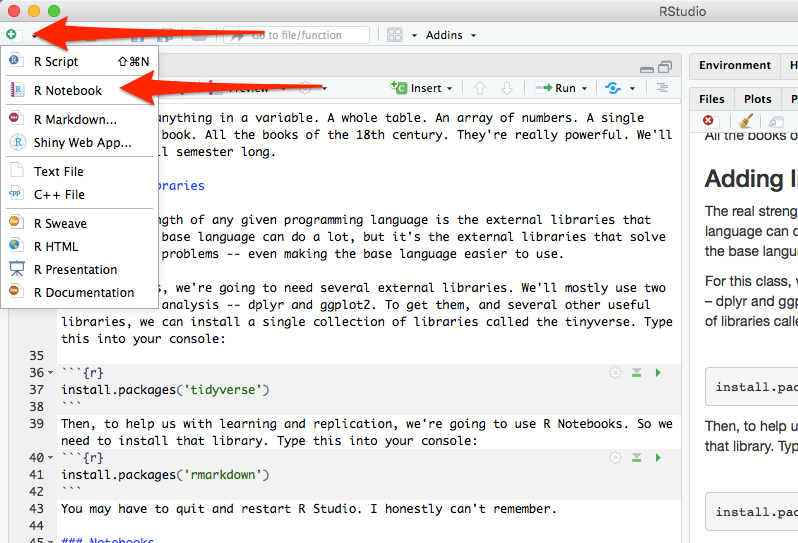
\includegraphics{./images/verybasics2.png}

In our first lab, we'll go through the process of editing a markdown
notebook.

\bookmarksetup{startatroot}

\hypertarget{aggregates}{%
\chapter{Aggregates}\label{aggregates}}

\hypertarget{libraries}{%
\section{Libraries}\label{libraries}}

R is a statistical programming language that is purpose built for data
analysis.

Base R does a lot, but there are a mountain of external libraries that
do things to make R better/easier/more fully featured. We already
installed the tidyverse -- or you should have if you followed the
instructions for the last assignment -- which isn't exactly a library,
but a collection of libraries. Together, they make up the Tidyverse.
Individually, they are extraordinarily useful for what they do. We can
load them all at once using the tidyverse name, or we can load them
individually. Let's start with individually.

The two libraries we are going to need for this assignment are
\texttt{readr} and \texttt{dplyr}. The library \texttt{readr} reads
different types of data in. For this assignment, we're going to read in
csv data or Comma Separated Values data. That's data that has a comma
between each column of data.

Then we're going to use \texttt{dplyr} to analyze it.

To use a library, you need to import it. Good practice -- one I'm going
to insist on -- is that you put all your library steps at the top of
your notebooks.

That code looks like this:

\begin{Shaded}
\begin{Highlighting}[]
\FunctionTok{library}\NormalTok{(readr)}
\end{Highlighting}
\end{Shaded}

To load them both, you need to do this:

\begin{Shaded}
\begin{Highlighting}[]
\FunctionTok{library}\NormalTok{(readr)}
\FunctionTok{library}\NormalTok{(dplyr)}
\end{Highlighting}
\end{Shaded}

\begin{verbatim}

Attaching package: 'dplyr'
\end{verbatim}

\begin{verbatim}
The following objects are masked from 'package:stats':

    filter, lag
\end{verbatim}

\begin{verbatim}
The following objects are masked from 'package:base':

    intersect, setdiff, setequal, union
\end{verbatim}

But, because those two libraries -- and several others that we're going
to use over the course of this class -- are so commonly used, there's a
shortcut to loading all of the libraries we'll need:

\begin{Shaded}
\begin{Highlighting}[]
\FunctionTok{library}\NormalTok{(tidyverse)}
\end{Highlighting}
\end{Shaded}

You can keep doing that for as many libraries as you need.

\hypertarget{importing-data}{%
\section{Importing data}\label{importing-data}}

The first thing we need to do is get some data to work with. We do that
by reading it in. In our case, we're going to read a datatable from an
``rds'' file, which is a format for storing data with R. Later in the
course, we'll more frequently work with a format called a CSV. A CSV is
a stripped down version of a spreadsheet you might open in a program
like Excel, in which each column is separated by a comma. RDS files are
less common when getting data from other people. But reading in CSVs is
less foolproof than reading in rds files, so for now we'll work with
rds.

The rds file we're going to read in contains individual campaign
contributions from Maryland donors via WinRed, an online fundraising
platform used by conservatives. We'll be working with a slice of the
data from earlier this year.

So step 1 is to import the data. The code to import the data looks like
this:

\texttt{maryland\_winred\_contributions\ \textless{}-\ read\_rds("maryland\_winred.rds")}

Let's unpack that.

The first part -- \textbf{maryland\_winred\_contributions} -- is the
name of a variable.

A \textbf{variable} is just a name that we'll use to refer to some more
complex thing. In this case, the more complex thing is the data we're
importing into R that will be stored as a \textbf{dataframe}, which is
one way R stores data.

We can call this variable whatever we want. The variable name doesn't
matter, technically. We could use any word. You could use your first
name, if you like. Generally, though, we want to give variables names
that are descriptive of the thing they refer to. Which is why we're
calling this one \textbf{maryland\_winred\_contributions}. Variable
names, by convention are one word all lower case (or two or more words
connected by an underscore). You can end a variable with a number, but
you can't start one with a number.

The \texttt{\textless{}-} bit, you'll recall from the basics, is the
\textbf{variable assignment operator}. It's how we know we're assigning
something to a word. Think of the arrow as saying ``Take everything on
the right of this arrow and stuff it into the thing on the left.'' So
we're creating an empty vessel called
\textbf{maryland\_winred\_contributions} and stuffing all this data into
it.

\textbf{read\_rds()} is a function, one that only works when we've
loaded the tidyverse. A \textbf{function} is a little bit of computer
code that takes in information and follows a series of pre-determined
steps and spits it back out. A recipe to make pizza is a kind of
function. We might call it \textbf{make\_pizza()}.

The function does one thing. It takes a preset collection of ingredients
-- flour, water, oil, cheese, tomato, salt -- and passes them through
each step outlined in a recipe, in order. Things like: mix flour and
water and oil, knead, let it sit, roll it out, put tomato sauce and
cheese on it, bake it in an oven, then take it out.

The output of our \textbf{make pizza()} function is a finished pie.

We'll make use of a lot of pre-written functions from the tidyverse and
other packages, and even write some of our own. Back to this line of
code:

\texttt{maryland\_winred\_contributions\ \textless{}-\ read\_rds("maryland\_winred.rds")}

Inside of the \textbf{read\_rds()} function, we've put the name of the
file we want to load. Things we put inside of function, to customize
what the function does, are called \textbf{arguments}.

The easiest thing to do, if you are confused about how to find your
data, is to put your data in the same folder as as your notebook (you'll
have to save that notebook first). If you do that, then you just need to
put the name of the file in there (maryland\_winred.rds). If you put
your data in a folder called ``data'' that sits next to your data
notebook, your function would instead look like this:

\begin{Shaded}
\begin{Highlighting}[]
\NormalTok{maryland\_winred\_contributions }\OtherTok{\textless{}{-}} \FunctionTok{read\_rds}\NormalTok{(}\StringTok{"data/maryland\_winred.rds"}\NormalTok{)}
\end{Highlighting}
\end{Shaded}

In this data set, each row represents an individual contribution to a
federal political committee, typically a candidate's campaign account.

After loading the data, it's a good idea to get a sense of its shape.
What does it look like? There are several ways we can examine it.

By looking in the R Studio environment window, we can see the number of
rows (called ``obs.'', which is short for observations), and the number
of columns(called variables). We can double click on the dataframe name
in the environment window, and explore it like a spreadsheet.

There are several useful functions for getting a sense of the dataset
right in our markdown document.

If we run \texttt{glimpse(maryland\_winred\_contributions)}, it will
give us a list of the columns, the data type for each column and and the
first few values for each column.

\begin{Shaded}
\begin{Highlighting}[]
\FunctionTok{glimpse}\NormalTok{(maryland\_winred\_contributions)}
\end{Highlighting}
\end{Shaded}

\begin{verbatim}
Rows: 54,247
Columns: 24
$ linenumber       <chr> "SA11AI", "SA11AI", "SA11AI", "SA11AI", "SA11AI", "SA~
$ fec_committee_id <chr> "C00694323", "C00694323", "C00694323", "C00694323", "~
$ tran_id          <chr> "A9EF36684A71C4FF097A", "A64BB5021801F42B386B", "A583~
$ flag_orgind      <chr> "IND", "IND", "IND", "IND", "IND", "IND", "IND", "IND~
$ org_name         <lgl> NA, NA, NA, NA, NA, NA, NA, NA, NA, NA, NA, NA, NA, N~
$ last_name        <chr> "Hansher", "Leishman", "Bode", "Gallagher", "Bode", "~
$ first_name       <chr> "Beth", "Alexander", "John", "Daniel", "Denise", "Joe~
$ middle_name      <lgl> NA, NA, NA, NA, NA, NA, NA, NA, NA, NA, NA, NA, NA, N~
$ prefix           <lgl> NA, NA, NA, NA, NA, NA, NA, NA, NA, NA, NA, NA, NA, N~
$ suffix           <lgl> NA, NA, NA, NA, NA, NA, NA, NA, NA, NA, NA, NA, NA, N~
$ address_one      <chr> "7205 Arrowood Rd", "1021 Gadsden Ave", "29389 Catalp~
$ address_two      <chr> NA, NA, NA, NA, NA, NA, NA, NA, NA, NA, NA, NA, NA, N~
$ city             <chr> "Bethesda", "Silver Spring", "Easton", "Towson", "Eas~
$ state            <chr> "MD", "MD", "MD", "MD", "MD", "MD", "MD", "MD", "MD",~
$ zip              <dbl> 20817, 20905, 21601, 21204, 21601, 20815, 21502, 2081~
$ prigen           <lgl> NA, NA, NA, NA, NA, NA, NA, NA, NA, NA, NA, NA, NA, N~
$ date             <date> 2022-06-01, 2022-05-25, 2022-06-16, 2022-04-05, 2022~
$ amount           <dbl> 5800.00, 5800.00, 5800.00, 5800.00, 5800.00, 5800.00,~
$ aggregate_amount <dbl> 5800.00, 22300.00, 11600.00, 17900.00, 17650.00, 1450~
$ employer         <chr> "INFORMATION REQUESTED", "RIVER", "CORN REFINERS ASSO~
$ occupation       <chr> "HOMEMAKER", "CEO", "ASSOCIATION EXECUTIVE", "CLO", "~
$ memo_code        <lgl> NA, NA, NA, NA, NA, NA, NA, NA, NA, NA, NA, NA, NA, N~
$ memo_text        <chr> "Earmarked for BLAKE MASTERS FOR SENATE (C00784165)",~
$ cycle            <dbl> 2022, 2022, 2022, 2022, 2022, 2022, 2022, 2022, 2022,~
\end{verbatim}

If we type \texttt{head(maryland\_winred\_contributions)}, it will print
out the columns and the first six rows of data.

\begin{Shaded}
\begin{Highlighting}[]
\FunctionTok{head}\NormalTok{(maryland\_winred\_contributions)}
\end{Highlighting}
\end{Shaded}

\begin{verbatim}
# A tibble: 6 x 24
  linenu~1 fec_c~2 tran_id flag_~3 org_n~4 last_~5 first~6 middl~7 prefix suffix
  <chr>    <chr>   <chr>   <chr>   <lgl>   <chr>   <chr>   <lgl>   <lgl>  <lgl> 
1 SA11AI   C00694~ A9EF36~ IND     NA      Hansher Beth    NA      NA     NA    
2 SA11AI   C00694~ A64BB5~ IND     NA      Leishm~ Alexan~ NA      NA     NA    
3 SA11AI   C00694~ A5835B~ IND     NA      Bode    John    NA      NA     NA    
4 SA11AI   C00694~ AE3AF0~ IND     NA      Gallag~ Daniel  NA      NA     NA    
5 SA11AI   C00694~ AC5569~ IND     NA      Bode    Denise  NA      NA     NA    
6 SA11AI   C00694~ A2B1EB~ IND     NA      Kaplan  Joel    NA      NA     NA    
# ... with 14 more variables: address_one <chr>, address_two <chr>, city <chr>,
#   state <chr>, zip <dbl>, prigen <lgl>, date <date>, amount <dbl>,
#   aggregate_amount <dbl>, employer <chr>, occupation <chr>, memo_code <lgl>,
#   memo_text <chr>, cycle <dbl>, and abbreviated variable names 1: linenumber,
#   2: fec_committee_id, 3: flag_orgind, 4: org_name, 5: last_name,
#   6: first_name, 7: middle_name
\end{verbatim}

We can also click on the data name in the R Studio environment window to
explore it interactively.

\hypertarget{group-by-and-count}{%
\section{Group by and count}\label{group-by-and-count}}

So what if we wanted to know how many contributions went to each
recipient?

To do that by hand, we'd have to take each of the 54,247 individual rows
(or observations or records) and sort them into a pile. We'd put them in
groups -- one for each recipient -- and then count them.

\texttt{dplyr} has a group by function in it that does just this. A
massive amount of data analysis involves grouping like things together
and then doing simple things like counting them, or averaging them
together. So it's a good place to start.

So to do this, we'll take our dataset and we'll introduce a new
operator: \texttt{\%\textgreater{}\%}. The best way to read that
operator, in my opinion, is to interpret that as ``and then do this.''

We're going to establish a pattern that will come up again and again
throughout this book: \texttt{data\ \%\textgreater{}\%\ function}. In
English: take your data set and then do this specific action to it.

The first step of every analysis starts with the data being used. Then
we apply functions to the data.

In our case, the pattern that you'll use many, many times is:
\texttt{data\ \%\textgreater{}\%\ group\_by(COLUMN\ NAME)\ \%\textgreater{}\%\ summarize(VARIABLE\ NAME\ =\ AGGREGATE\ FUNCTION(COLUMN\ NAME))}

In our dataset, the column with recipient information is called
``memo\_text''

Here's the code to count the number of contributions to each recipient:

\begin{Shaded}
\begin{Highlighting}[]
\NormalTok{maryland\_winred\_contributions }\SpecialCharTok{\%\textgreater{}\%}
  \FunctionTok{group\_by}\NormalTok{(memo\_text) }\SpecialCharTok{\%\textgreater{}\%}
  \FunctionTok{summarise}\NormalTok{(}
    \AttributeTok{count\_contribs =} \FunctionTok{n}\NormalTok{()}
\NormalTok{  )}
\end{Highlighting}
\end{Shaded}

\begin{verbatim}
# A tibble: 519 x 2
   memo_text                                           count_contribs
   <chr>                                                        <int>
 1 Earmarked for ABRAHAM LINCOLN PAC (C00631051)                    3
 2 Earmarked for ADRIAN SMITH FOR CONGRESS (C00412890)              2
 3 Earmarked for AL FOR MONTANA (C00783381)                         1
 4 Earmarked for ALAMO PAC (C00387464)                              1
 5 Earmarked for ALAN SIMS FOR CONGRESS (C00784975)                 2
 6 Earmarked for ALASKANS FOR DAN SULLIVAN (C00570994)              5
 7 Earmarked for ALASKANS FOR NICK BEGICH (C00792341)               1
 8 Earmarked for ALEK FOR OREGON (C00715854)                      121
 9 Earmarked for ALEX FOR CONGRESS (C00771279)                      3
10 Earmarked for ALLCORN FOR COLORADO (C00798983)                   2
# ... with 509 more rows
\end{verbatim}

So let's walk through that.

We start with our dataset -- \texttt{maryland\_winred\_contributions} --
and then we tell it to group the data by a given field in the data. In
this case, we wanted to group together all the recipients, signified by
the field name \texttt{memo\_text}, which you could get from using the
glimpse() function. After we group the data, we need to count them up.

In dplyr, we use the \texttt{summarize()} function,
\href{http://dplyr.tidyverse.org/reference/summarise.html}{which can do
alot more than just count things}.

Inside the parentheses in summarize, we set up the summaries we want. In
this case, we just want a count of the number of loans for each county
grouping. The line of code \texttt{count\_contribs\ =\ n(),} says create
a new field, called \texttt{count\_contribs} and set it equal to
\texttt{n()}. \texttt{n()} is a function that counts the number of rows
or records in each group. Why the letter n? The letter n is a common
symbol used to denote a count of something. The number of things (or
rows or observations or records) in a dataset? Statisticians call it
n.~There are n number of contributions in this dataset.

When we run that, we get a list of recipients with a count next to them.
But it's not in any order.

So we'll add another ``and then do this'' symbol -- \%\textgreater\% --
and use a new function called \texttt{arrange()}. Arrange does what you
think it does -- it arranges data in order. By default, it's in
ascending order -- smallest to largest. But if we want to know the
county with the most loans, we need to sort it in descending order. That
looks like this:

\begin{Shaded}
\begin{Highlighting}[]
\NormalTok{maryland\_winred\_contributions }\SpecialCharTok{\%\textgreater{}\%}
  \FunctionTok{group\_by}\NormalTok{(memo\_text) }\SpecialCharTok{\%\textgreater{}\%}
  \FunctionTok{summarise}\NormalTok{(}
    \AttributeTok{count\_contribs =} \FunctionTok{n}\NormalTok{()}
\NormalTok{  ) }\SpecialCharTok{\%\textgreater{}\%}
  \FunctionTok{arrange}\NormalTok{(}\FunctionTok{desc}\NormalTok{(count\_contribs))}
\end{Highlighting}
\end{Shaded}

\begin{verbatim}
# A tibble: 519 x 2
   memo_text                                                          count_co~1
   <chr>                                                                   <int>
 1 Earmarked for SAVE AMERICA JOINT FUNDRAISING COMMITTEE (C00770941)       7809
 2 Earmarked for NRSC (C00027466)                                           6497
 3 Earmarked for REPUBLICAN NATIONAL COMMITTEE (C00003418)                  4268
 4 Earmarked for NRCC (C00075820)                                           3945
 5 Earmarked for TEAM SCALISE (C00750521)                                   2477
 6 Earmarked for KEVIN MCCARTHY FOR CONGRESS (C00420935)                    1461
 7 Earmarked for MARCO RUBIO FOR SENATE (C00620518)                         1326
 8 Earmarked for RON JOHNSON FOR SENATE, INC. (C00482984)                    974
 9 Earmarked for JOHN KENNEDY FOR US (C00608398)                             955
10 Earmarked for TIM SCOTT FOR SENATE (C00540302)                            915
# ... with 509 more rows, and abbreviated variable name 1: count_contribs
\end{verbatim}

The Save America Joint Fundraising Committee has 7,809 contributions,
more than any other recipient.

We can, if we want, group by more than one thing.

The WinRed data contains a column detailing the date of the
contribution: ``date''.

We can group by ``memo\_text'' and ``date'' to see how many
contributions occurred on every date to every recipient. We'll sort by
recipient and then date

\begin{Shaded}
\begin{Highlighting}[]
\NormalTok{maryland\_winred\_contributions }\SpecialCharTok{\%\textgreater{}\%}
  \FunctionTok{group\_by}\NormalTok{(memo\_text, date) }\SpecialCharTok{\%\textgreater{}\%}
  \FunctionTok{summarise}\NormalTok{(}
    \AttributeTok{count\_contribs =} \FunctionTok{n}\NormalTok{()}
\NormalTok{  ) }\SpecialCharTok{\%\textgreater{}\%}
  \FunctionTok{arrange}\NormalTok{(memo\_text, date)}
\end{Highlighting}
\end{Shaded}

\begin{verbatim}
`summarise()` has grouped output by 'memo_text'. You can override using the
`.groups` argument.
\end{verbatim}

\begin{verbatim}
# A tibble: 9,194 x 3
# Groups:   memo_text [519]
   memo_text                                           date       count_contribs
   <chr>                                               <date>              <int>
 1 Earmarked for ABRAHAM LINCOLN PAC (C00631051)       2022-06-27              1
 2 Earmarked for ABRAHAM LINCOLN PAC (C00631051)       2022-06-28              1
 3 Earmarked for ABRAHAM LINCOLN PAC (C00631051)       2022-06-30              1
 4 Earmarked for ADRIAN SMITH FOR CONGRESS (C00412890) 2022-04-01              1
 5 Earmarked for ADRIAN SMITH FOR CONGRESS (C00412890) 2022-06-27              1
 6 Earmarked for AL FOR MONTANA (C00783381)            2022-06-04              1
 7 Earmarked for ALAMO PAC (C00387464)                 2022-05-16              1
 8 Earmarked for ALAN SIMS FOR CONGRESS (C00784975)    2022-04-23              1
 9 Earmarked for ALAN SIMS FOR CONGRESS (C00784975)    2022-05-23              1
10 Earmarked for ALASKANS FOR DAN SULLIVAN (C00570994) 2022-04-22              1
# ... with 9,184 more rows
\end{verbatim}

\hypertarget{other-summarization-methods-summing-mean-median-min-and-max}{%
\section{Other summarization methods: summing, mean, median, min and
max}\label{other-summarization-methods-summing-mean-median-min-and-max}}

In the last example, we grouped like records together and counted them,
but there's so much more we can to summarize each group.

Let's say we wanted to know the total dollar amount of contributions to
each recipient? For that, we could use the \texttt{sum()} function to
add up all of the loan values in the column ``amount''. We put the
column we want to total -- ``amount'' -- inside the sum() function
\texttt{sum(amount)}. Note that we can simply add a new summarize
function here, keeping our count\_contribs field in our output table.

\begin{Shaded}
\begin{Highlighting}[]
\NormalTok{maryland\_winred\_contributions }\SpecialCharTok{\%\textgreater{}\%}
  \FunctionTok{group\_by}\NormalTok{(memo\_text) }\SpecialCharTok{\%\textgreater{}\%}
  \FunctionTok{summarise}\NormalTok{(}
    \AttributeTok{count\_contribs =} \FunctionTok{n}\NormalTok{(),}
    \AttributeTok{total\_amount =} \FunctionTok{sum}\NormalTok{(amount)}
\NormalTok{  ) }\SpecialCharTok{\%\textgreater{}\%}
  \FunctionTok{arrange}\NormalTok{(}\FunctionTok{desc}\NormalTok{(total\_amount))}
\end{Highlighting}
\end{Shaded}

\begin{verbatim}
# A tibble: 519 x 3
   memo_text                                                     count~1 total~2
   <chr>                                                           <int>   <dbl>
 1 Earmarked for SAVE AMERICA JOINT FUNDRAISING COMMITTEE (C007~    7809 220155.
 2 Earmarked for NRSC (C00027466)                                   6497 149673.
 3 Earmarked for NRCC (C00075820)                                   3945 118658.
 4 Earmarked for REPUBLICAN NATIONAL COMMITTEE (C00003418)          4268 111955.
 5 Earmarked for NICOLEE AMBROSE FOR CONGRESS (C00812891)            150  67980.
 6 Earmarked for TEAM SCALISE (C00750521)                           2477  51709.
 7 Earmarked for PARROTT FOR CONGRESS (C00691931)                    346  45243.
 8 Earmarked for MARCO RUBIO FOR SENATE (C00620518)                 1326  43279.
 9 Earmarked for KEVIN MCCARTHY FOR CONGRESS (C00420935)            1461  29612.
10 Earmarked for RON JOHNSON FOR SENATE, INC. (C00482984)            974  29611.
# ... with 509 more rows, and abbreviated variable names 1: count_contribs,
#   2: total_amount
\end{verbatim}

We can also calculate the average amount for each recipient -- the mean
-- and the amount that sits at the midpoint of our data -- the median.

\begin{Shaded}
\begin{Highlighting}[]
\NormalTok{maryland\_winred\_contributions }\SpecialCharTok{\%\textgreater{}\%}
  \FunctionTok{group\_by}\NormalTok{(memo\_text) }\SpecialCharTok{\%\textgreater{}\%}
  \FunctionTok{summarise}\NormalTok{(}
    \AttributeTok{count\_contribs =} \FunctionTok{n}\NormalTok{(),}
    \AttributeTok{total\_amount =} \FunctionTok{sum}\NormalTok{(amount),}
    \AttributeTok{mean\_amount =} \FunctionTok{mean}\NormalTok{(amount),}
    \AttributeTok{median\_amount =} \FunctionTok{median}\NormalTok{(amount)}
\NormalTok{  ) }\SpecialCharTok{\%\textgreater{}\%}
  \FunctionTok{arrange}\NormalTok{(}\FunctionTok{desc}\NormalTok{(count\_contribs))}
\end{Highlighting}
\end{Shaded}

\begin{verbatim}
# A tibble: 519 x 5
   memo_text                                     count~1 total~2 mean_~3 media~4
   <chr>                                           <int>   <dbl>   <dbl>   <dbl>
 1 Earmarked for SAVE AMERICA JOINT FUNDRAISING~    7809 220155.    28.2    20  
 2 Earmarked for NRSC (C00027466)                   6497 149673.    23.0    12.5
 3 Earmarked for REPUBLICAN NATIONAL COMMITTEE ~    4268 111955.    26.2    18  
 4 Earmarked for NRCC (C00075820)                   3945 118658.    30.1    25  
 5 Earmarked for TEAM SCALISE (C00750521)           2477  51709.    20.9    10  
 6 Earmarked for KEVIN MCCARTHY FOR CONGRESS (C~    1461  29612.    20.3    10  
 7 Earmarked for MARCO RUBIO FOR SENATE (C00620~    1326  43279.    32.6    20.2
 8 Earmarked for RON JOHNSON FOR SENATE, INC. (~     974  29611.    30.4    25  
 9 Earmarked for JOHN KENNEDY FOR US (C00608398)     955  26433.    27.7    15  
10 Earmarked for TIM SCOTT FOR SENATE (C0054030~     915  29095.    31.8    10  
# ... with 509 more rows, and abbreviated variable names 1: count_contribs,
#   2: total_amount, 3: mean_amount, 4: median_amount
\end{verbatim}

We see something interesting here. The mean contribution amount is
higher than the median amount in most cases, but the difference isn't
huge. In some cases the mean gets skewed by larger amounts. Examining
both the median -- which is less sensitive to extreme values -- and the
mean -- which is more sensitive to extreme values -- gives you a clearer
picture of the composition of the data.

What about the highest and lowest amounts for each recipient? For that,
we can use the \texttt{min()} and \texttt{max()} functions.

\begin{Shaded}
\begin{Highlighting}[]
\NormalTok{maryland\_winred\_contributions }\SpecialCharTok{\%\textgreater{}\%}
  \FunctionTok{group\_by}\NormalTok{(memo\_text) }\SpecialCharTok{\%\textgreater{}\%}
  \FunctionTok{summarise}\NormalTok{(}
    \AttributeTok{count\_contribs =} \FunctionTok{n}\NormalTok{(),}
    \AttributeTok{total\_amount =} \FunctionTok{sum}\NormalTok{(amount),}
    \AttributeTok{mean\_amount =} \FunctionTok{mean}\NormalTok{(amount),}
    \AttributeTok{median\_amount =} \FunctionTok{median}\NormalTok{(amount),}
    \AttributeTok{min\_amount =} \FunctionTok{min}\NormalTok{(amount),}
    \AttributeTok{max\_amount =} \FunctionTok{max}\NormalTok{(amount)}
\NormalTok{  ) }\SpecialCharTok{\%\textgreater{}\%}
  \FunctionTok{arrange}\NormalTok{(}\FunctionTok{desc}\NormalTok{(max\_amount))}
\end{Highlighting}
\end{Shaded}

\begin{verbatim}
# A tibble: 519 x 7
   memo_text                     count~1 total~2 mean_~3 media~4 min_a~5 max_a~6
   <chr>                           <int>   <dbl>   <dbl>   <dbl>   <dbl>   <dbl>
 1 Earmarked for ALASKANS FOR D~       5   7304   1461.      500    1       5800
 2 Earmarked for AMAL FOR CONGR~      30  10442.   348.       25    1       5800
 3 Earmarked for BLAKE MASTERS ~      24   6780    282.       25   10       5800
 4 Earmarked for FRIENDS OF MIK~     358  17711.    49.5      10    0.5     5800
 5 Earmarked for FRIENDS OF TOD~      75  14833.   198.        5    0.2     5800
 6 Earmarked for GALLUCH FOR CO~       1   5800   5800      5800 5800       5800
 7 Earmarked for KELLY FOR ALAS~      54   7900    146.       25    5       5800
 8 Earmarked for LAWLER FOR CON~       1   5800   5800      5800 5800       5800
 9 Earmarked for LAXALT FOR SEN~     334  26920.    80.6      25    0.77    5800
10 Earmarked for MCHENRY FOR CO~       3   6800   2267.      500  500       5800
# ... with 509 more rows, and abbreviated variable names 1: count_contribs,
#   2: total_amount, 3: mean_amount, 4: median_amount, 5: min_amount,
#   6: max_amount
\end{verbatim}

From this, we can see that some committees focus on small-dollar donors
while others ask for (and get) larger amounts. This pattern isn't
random: campaigns make choices about how they will raise money.

It would be interesting to see what the largest donation was. To do
that, we could simply take our original data set and sort it from
highest to lowest on the amount.

\begin{Shaded}
\begin{Highlighting}[]
\NormalTok{maryland\_winred\_contributions }\SpecialCharTok{\%\textgreater{}\%}
  \FunctionTok{arrange}\NormalTok{(}\FunctionTok{desc}\NormalTok{(amount))}
\end{Highlighting}
\end{Shaded}

\begin{verbatim}
# A tibble: 54,247 x 24
   linen~1 fec_c~2 tran_id flag_~3 org_n~4 last_~5 first~6 middl~7 prefix suffix
   <chr>   <chr>   <chr>   <chr>   <lgl>   <chr>   <chr>   <lgl>   <lgl>  <lgl> 
 1 SA11AI  C00694~ A9EF36~ IND     NA      Hansher Beth    NA      NA     NA    
 2 SA11AI  C00694~ A64BB5~ IND     NA      Leishm~ Alexan~ NA      NA     NA    
 3 SA11AI  C00694~ A5835B~ IND     NA      Bode    John    NA      NA     NA    
 4 SA11AI  C00694~ AE3AF0~ IND     NA      Gallag~ Daniel  NA      NA     NA    
 5 SA11AI  C00694~ AC5569~ IND     NA      Bode    Denise  NA      NA     NA    
 6 SA11AI  C00694~ A2B1EB~ IND     NA      Kaplan  Joel    NA      NA     NA    
 7 SA11AI  C00694~ A2D9CC~ IND     NA      Freas   Dustin  NA      NA     NA    
 8 SA11AI  C00694~ A8F4D9~ IND     NA      Monahan Tom     NA      NA     NA    
 9 SA11AI  C00694~ A3E262~ IND     NA      powers  rick    NA      NA     NA    
10 SA11AI  C00694~ AD5034~ IND     NA      JonesL~ Brien   NA      NA     NA    
# ... with 54,237 more rows, 14 more variables: address_one <chr>,
#   address_two <chr>, city <chr>, state <chr>, zip <dbl>, prigen <lgl>,
#   date <date>, amount <dbl>, aggregate_amount <dbl>, employer <chr>,
#   occupation <chr>, memo_code <lgl>, memo_text <chr>, cycle <dbl>, and
#   abbreviated variable names 1: linenumber, 2: fec_committee_id,
#   3: flag_orgind, 4: org_name, 5: last_name, 6: first_name, 7: middle_name
\end{verbatim}

Lots of \$5,800 contributions, which probably seems like a weirdly
specific number. And it is! That's the maximum contribution an
individual can give for both a primary and a general election.

\bookmarksetup{startatroot}

\hypertarget{mutating-data}{%
\chapter{Mutating data}\label{mutating-data}}

Often the data you have will prompt questions that it doesn't
immediately answer. The PPP loan applications include a total amount
column but also columns for different categories the money would be used
for: payroll, utilities, rent, etc. Amounts are great, but comparing
absolute numbers to each other is only useful if you have a very small
number. We need percentages!

To do that in R, we can use \texttt{dplyr} and \texttt{mutate} to
calculate new metrics in a new field using existing fields of data.
That's the essence of \texttt{mutate} - using the data you have to
answer a new question.

So first we'll import the tidyverse so we can read in our data and begin
to work with it.

\begin{Shaded}
\begin{Highlighting}[]
\FunctionTok{library}\NormalTok{(tidyverse)}
\end{Highlighting}
\end{Shaded}

Now we'll import a dataset of county-level election results from
Maryland's 2018 primary that is in the data folder in this chapter's
pre-lab directory. We'll use this to explore ways to create new
information from existing data.

\begin{Shaded}
\begin{Highlighting}[]
\NormalTok{primary\_18 }\OtherTok{\textless{}{-}} \FunctionTok{read\_csv}\NormalTok{(}\StringTok{\textquotesingle{}data/maryland\_primary\_2018.csv\textquotesingle{}}\NormalTok{)}
\end{Highlighting}
\end{Shaded}

\begin{verbatim}
Rows: 1778 Columns: 15
-- Column specification --------------------------------------------------------
Delimiter: ","
chr  (7): election_type, result_type, office, district, name_raw, party, jur...
dbl  (6): votes, year, election_day, absentee, provisional, second_absentee
lgl  (1): special
dttm (1): end_date

i Use `spec()` to retrieve the full column specification for this data.
i Specify the column types or set `show_col_types = FALSE` to quiet this message.
\end{verbatim}

First, let's add a column called \texttt{percent\_election\_day} for the
percentage of votes that were cast on election day for each candidate
result in a county. The code to calculate a percentage is pretty simple.
Remember, with \texttt{summarize}, we used \texttt{n()} to count things.
With \texttt{mutate}, we use very similar syntax to calculate a new
value -- a new column of data -- using other values in our dataset.

If we look at what we got when we imported the data, you'll see there's
\texttt{election\_day} as the numerator, and we'll use \texttt{votes} as
the denominator. We can simply things by only selecting a few columns.

\begin{Shaded}
\begin{Highlighting}[]
\NormalTok{primary\_18 }\SpecialCharTok{\%\textgreater{}\%}
  \FunctionTok{select}\NormalTok{(office, district, name\_raw, party, jurisdiction, election\_day, votes) }\SpecialCharTok{\%\textgreater{}\%}
  \FunctionTok{mutate}\NormalTok{(}
  \AttributeTok{percent\_election\_day =}\NormalTok{ election\_day}\SpecialCharTok{/}\NormalTok{votes}
\NormalTok{)}
\end{Highlighting}
\end{Shaded}

\begin{verbatim}
# A tibble: 1,778 x 8
   office                  district name_raw party juris~1 elect~2 votes perce~3
   <chr>                   <chr>    <chr>    <chr> <chr>     <dbl> <dbl>   <dbl>
 1 Governor / Lt. Governor <NA>     Rushern~ DEM   Allega~     324   413   0.785
 2 Governor / Lt. Governor <NA>     Ralph J~ DEM   Allega~     106   122   0.869
 3 Governor / Lt. Governor <NA>     Ben Jea~ DEM   Allega~     979  1170   0.837
 4 Governor / Lt. Governor <NA>     James H~ DEM   Allega~      99   106   0.934
 5 Governor / Lt. Governor <NA>     Valerie~ DEM   Allega~     118   159   0.742
 6 Governor / Lt. Governor <NA>     Rich Ma~ DEM   Allega~     133   169   0.787
 7 Governor / Lt. Governor <NA>     Alec Ro~ DEM   Allega~     175   218   0.803
 8 Governor / Lt. Governor <NA>     Jim Shea DEM   Allega~     239   284   0.842
 9 Governor / Lt. Governor <NA>     Krish O~ DEM   Allega~     364   462   0.788
10 Comptroller             <NA>     Peter F~ DEM   Allega~    2518  3077   0.818
# ... with 1,768 more rows, and abbreviated variable names 1: jurisdiction,
#   2: election_day, 3: percent_election_day
\end{verbatim}

Now we've got our \texttt{percent\_election\_day} column. But what do
you see right away? Do those numbers look like we expect them to?
No.~They're a decimal expressed as a percentage. So let's fix that by
multiplying by 100.

\begin{Shaded}
\begin{Highlighting}[]
\NormalTok{primary\_18 }\SpecialCharTok{\%\textgreater{}\%}
  \FunctionTok{select}\NormalTok{(office, district, name\_raw, party, jurisdiction, election\_day, votes) }\SpecialCharTok{\%\textgreater{}\%}
  \FunctionTok{mutate}\NormalTok{(}
  \AttributeTok{percent\_election\_day =}\NormalTok{ (election\_day}\SpecialCharTok{/}\NormalTok{votes)}\SpecialCharTok{*}\DecValTok{100}
\NormalTok{)}
\end{Highlighting}
\end{Shaded}

\begin{verbatim}
# A tibble: 1,778 x 8
   office                  district name_raw party juris~1 elect~2 votes perce~3
   <chr>                   <chr>    <chr>    <chr> <chr>     <dbl> <dbl>   <dbl>
 1 Governor / Lt. Governor <NA>     Rushern~ DEM   Allega~     324   413    78.5
 2 Governor / Lt. Governor <NA>     Ralph J~ DEM   Allega~     106   122    86.9
 3 Governor / Lt. Governor <NA>     Ben Jea~ DEM   Allega~     979  1170    83.7
 4 Governor / Lt. Governor <NA>     James H~ DEM   Allega~      99   106    93.4
 5 Governor / Lt. Governor <NA>     Valerie~ DEM   Allega~     118   159    74.2
 6 Governor / Lt. Governor <NA>     Rich Ma~ DEM   Allega~     133   169    78.7
 7 Governor / Lt. Governor <NA>     Alec Ro~ DEM   Allega~     175   218    80.3
 8 Governor / Lt. Governor <NA>     Jim Shea DEM   Allega~     239   284    84.2
 9 Governor / Lt. Governor <NA>     Krish O~ DEM   Allega~     364   462    78.8
10 Comptroller             <NA>     Peter F~ DEM   Allega~    2518  3077    81.8
# ... with 1,768 more rows, and abbreviated variable names 1: jurisdiction,
#   2: election_day, 3: percent_election_day
\end{verbatim}

Now, does this ordering do anything for us? No.~Let's fix that with
arrange.

\begin{Shaded}
\begin{Highlighting}[]
\NormalTok{primary\_18 }\SpecialCharTok{\%\textgreater{}\%}
  \FunctionTok{select}\NormalTok{(office, district, name\_raw, party, jurisdiction, election\_day, votes) }\SpecialCharTok{\%\textgreater{}\%}
  \FunctionTok{mutate}\NormalTok{(}
  \AttributeTok{percent\_election\_day =}\NormalTok{ (election\_day}\SpecialCharTok{/}\NormalTok{votes)}\SpecialCharTok{*}\DecValTok{100}
\NormalTok{)  }\SpecialCharTok{\%\textgreater{}\%} \FunctionTok{arrange}\NormalTok{(}\FunctionTok{desc}\NormalTok{(percent\_election\_day))}
\end{Highlighting}
\end{Shaded}

\begin{verbatim}
# A tibble: 1,778 x 8
   office                    distr~1 name_~2 party juris~3 elect~4 votes perce~5
   <chr>                     <chr>   <chr>   <chr> <chr>     <dbl> <dbl>   <dbl>
 1 U.S. Senator              <NA>    Erik J~ DEM   Garrett       8     8   100  
 2 U.S. Senator              <NA>    Albert~ REP   Allega~      69    71    97.2
 3 House of Delegates        01A     James ~ REP   Allega~     140   148    94.6
 4 Governor / Lt. Governor   <NA>    James ~ DEM   Allega~      99   106    93.4
 5 House of Delegates        38C     Jim Sh~ REP   Wicomi~      23    25    92  
 6 House of Delegates        01A     Wendel~ REP   Allega~     947  1031    91.9
 7 U.S. Senator              <NA>    Richar~ DEM   Garrett      11    12    91.7
 8 U.S. Senator              <NA>    Christ~ REP   Allega~     863   948    91.0
 9 U.S. Senator              <NA>    Marcia~ DEM   Allega~     113   125    90.4
10 Representative in Congre~ 06      Christ~ DEM   Allega~      37    41    90.2
# ... with 1,768 more rows, and abbreviated variable names 1: district,
#   2: name_raw, 3: jurisdiction, 4: election_day, 5: percent_election_day
\end{verbatim}

So now we have results ordered by \texttt{percent\_election\_day} with
the highest percentage first. To see the lowest percentage first, we can
reverse that \texttt{arrange} function.

\begin{Shaded}
\begin{Highlighting}[]
\NormalTok{primary\_18 }\SpecialCharTok{\%\textgreater{}\%}
  \FunctionTok{select}\NormalTok{(office, district, name\_raw, party, jurisdiction, election\_day, votes) }\SpecialCharTok{\%\textgreater{}\%}
  \FunctionTok{mutate}\NormalTok{(}
  \AttributeTok{percent\_election\_day =}\NormalTok{ (election\_day}\SpecialCharTok{/}\NormalTok{votes)}\SpecialCharTok{*}\DecValTok{100}
\NormalTok{)  }\SpecialCharTok{\%\textgreater{}\%} \FunctionTok{arrange}\NormalTok{(percent\_election\_day)}
\end{Highlighting}
\end{Shaded}

\begin{verbatim}
# A tibble: 1,778 x 8
   office                    distr~1 name_~2 party juris~3 elect~4 votes perce~5
   <chr>                     <chr>   <chr>   <chr> <chr>     <dbl> <dbl>   <dbl>
 1 Governor / Lt. Governor   <NA>    Valeri~ DEM   Talbot       38    89    42.7
 2 Governor / Lt. Governor   <NA>    Rich M~ DEM   Talbot       84   192    43.8
 3 Governor / Lt. Governor   <NA>    Rich M~ DEM   Kent         40    85    47.1
 4 Governor / Lt. Governor   <NA>    Rich M~ DEM   Garrett      32    67    47.8
 5 Governor / Lt. Governor   <NA>    Jim Sh~ DEM   Talbot      168   345    48.7
 6 U.S. Senator              <NA>    Blaine~ REP   Talbot       41    84    48.8
 7 House of Delegates        43      Urcill~ DEM   Baltim~     550  1122    49.0
 8 Governor / Lt. Governor   <NA>    Rusher~ DEM   Talbot      286   577    49.6
 9 House of Delegates        21      Mary A~ DEM   Anne A~     407   816    49.9
10 Representative in Congre~ 06      Christ~ DEM   Garrett       3     6    50  
# ... with 1,768 more rows, and abbreviated variable names 1: district,
#   2: name_raw, 3: jurisdiction, 4: election_day, 5: percent_election_day
\end{verbatim}

Only a handful of candidates got less than 50 percent of their total
votes in a county on election day. What a difference a pandemic makes.

\hypertarget{another-use-of-mutate}{%
\section{Another use of mutate}\label{another-use-of-mutate}}

Mutate is also useful for standardizing data - for example, making
different spellings of, say, cities into a single one.

Let's load some campaign contribution data - in this case Maryland
donors to Republican committees via WinRed's online platform earlier
this year - and take a look at the \texttt{city} column in our data.

\begin{Shaded}
\begin{Highlighting}[]
\NormalTok{maryland\_cities }\OtherTok{\textless{}{-}} \FunctionTok{read\_csv}\NormalTok{(}\StringTok{"data/winred\_md\_cities.csv"}\NormalTok{)}
\end{Highlighting}
\end{Shaded}

\begin{verbatim}
Rows: 408 Columns: 3
-- Column specification --------------------------------------------------------
Delimiter: ","
chr (1): city
dbl (2): count, sum

i Use `spec()` to retrieve the full column specification for this data.
i Specify the column types or set `show_col_types = FALSE` to quiet this message.
\end{verbatim}

You'll notice that there's a mix of styles: ``Baltimore'' and
``BALTIMORE'' for example. R will think those are two different cities,
and that will mean that any aggregates we create based on city won't be
accurate.

So how can we fix that? Mutate - it's not just for math! And a function
called \texttt{str\_to\_upper} that will convert a character column into
all uppercase. Now we can say exactly how many donations came from
Baltimore (I mean, of course, BALTIMORE).

\begin{Shaded}
\begin{Highlighting}[]
\NormalTok{standardized\_maryland\_cities }\OtherTok{\textless{}{-}}\NormalTok{ maryland\_cities }\SpecialCharTok{\%\textgreater{}\%}
  \FunctionTok{mutate}\NormalTok{(}
    \AttributeTok{upper\_city =} \FunctionTok{str\_to\_upper}\NormalTok{(city)}
\NormalTok{)}
\end{Highlighting}
\end{Shaded}

There are lots of potential uses for standardization - addresses, zip
codes, anything that can be misspelled or abbreviated.

\hypertarget{a-more-powerful-use}{%
\section{A more powerful use}\label{a-more-powerful-use}}

Mutate is even more useful when combined with some additional functions.
Let's focus on individual contributions from Maryland donors via WinRed;
we'd like to group their donations by amount into one of four
categories:

\begin{enumerate}
\def\labelenumi{\arabic{enumi}.}
\tightlist
\item
  Under \$100
\item
  \$101-\$499
\item
  \$500-\$2,900
\item
  More than \$2,901
\end{enumerate}

Mutate can make that happen by creating a new column and putting in a
category value \emph{based on the amount} of each record. First, let's
load the individual contributions:

\begin{Shaded}
\begin{Highlighting}[]
\NormalTok{maryland\_winred }\OtherTok{\textless{}{-}} \FunctionTok{read\_csv}\NormalTok{(}\StringTok{"data/winred\_md\_q2\_2022.csv"}\NormalTok{)}
\end{Highlighting}
\end{Shaded}

\begin{verbatim}
Rows: 54247 Columns: 24
-- Column specification --------------------------------------------------------
Delimiter: ","
chr  (13): linenumber, fec_committee_id, tran_id, flag_orgind, last_name, fi...
dbl   (4): zip, amount, aggregate_amount, cycle
lgl   (6): org_name, middle_name, prefix, suffix, prigen, memo_code
date  (1): date

i Use `spec()` to retrieve the full column specification for this data.
i Specify the column types or set `show_col_types = FALSE` to quiet this message.
\end{verbatim}

\begin{Shaded}
\begin{Highlighting}[]
\FunctionTok{head}\NormalTok{(maryland\_winred)}
\end{Highlighting}
\end{Shaded}

\begin{verbatim}
# A tibble: 6 x 24
  linenu~1 fec_c~2 tran_id flag_~3 org_n~4 last_~5 first~6 middl~7 prefix suffix
  <chr>    <chr>   <chr>   <chr>   <lgl>   <chr>   <chr>   <lgl>   <lgl>  <lgl> 
1 SA11AI   C00694~ A9EF36~ IND     NA      Hansher Beth    NA      NA     NA    
2 SA11AI   C00694~ A64BB5~ IND     NA      Leishm~ Alexan~ NA      NA     NA    
3 SA11AI   C00694~ A5835B~ IND     NA      Bode    John    NA      NA     NA    
4 SA11AI   C00694~ AE3AF0~ IND     NA      Gallag~ Daniel  NA      NA     NA    
5 SA11AI   C00694~ AC5569~ IND     NA      Bode    Denise  NA      NA     NA    
6 SA11AI   C00694~ A2B1EB~ IND     NA      Kaplan  Joel    NA      NA     NA    
# ... with 14 more variables: address_one <chr>, address_two <chr>, city <chr>,
#   state <chr>, zip <dbl>, prigen <lgl>, date <date>, amount <dbl>,
#   aggregate_amount <dbl>, employer <chr>, occupation <chr>, memo_code <lgl>,
#   memo_text <chr>, cycle <dbl>, and abbreviated variable names 1: linenumber,
#   2: fec_committee_id, 3: flag_orgind, 4: org_name, 5: last_name,
#   6: first_name, 7: middle_name
\end{verbatim}

Now that we've gotten a look, we can use \texttt{case\_when} to give our
new category column a value using some standard numeric logic:

\begin{Shaded}
\begin{Highlighting}[]
\NormalTok{maryland\_winred\_categories }\OtherTok{\textless{}{-}}\NormalTok{ maryland\_winred }\SpecialCharTok{\%\textgreater{}\%}
  \FunctionTok{mutate}\NormalTok{(}
    \AttributeTok{amount\_category =} \FunctionTok{case\_when}\NormalTok{(}
\NormalTok{        amount }\SpecialCharTok{\textless{}} \DecValTok{100} \SpecialCharTok{\textasciitilde{}} \StringTok{"Less than $100"}\NormalTok{,}
\NormalTok{        amount }\SpecialCharTok{\textgreater{}=} \DecValTok{100} \SpecialCharTok{\&}\NormalTok{ amount }\SpecialCharTok{\textless{}=} \DecValTok{500} \SpecialCharTok{\textasciitilde{}} \StringTok{"Between $100 and $500"}\NormalTok{,}
\NormalTok{        amount }\SpecialCharTok{\textgreater{}} \DecValTok{500} \SpecialCharTok{\&}\NormalTok{ amount }\SpecialCharTok{\textless{}=} \DecValTok{2900} \SpecialCharTok{\textasciitilde{}} \StringTok{"Between $501 and $2900"}\NormalTok{,}
\NormalTok{        amount }\SpecialCharTok{\textgreater{}} \DecValTok{2900} \SpecialCharTok{\textasciitilde{}} \StringTok{"More than $2,900"}
\NormalTok{      )}
\NormalTok{  )}
\end{Highlighting}
\end{Shaded}

We can then use our new \texttt{amount\_category} column in group\_by
statements to make summarizing easier:

\begin{Shaded}
\begin{Highlighting}[]
\NormalTok{maryland\_winred\_categories }\SpecialCharTok{\%\textgreater{}\%}
  \FunctionTok{group\_by}\NormalTok{(amount\_category) }\SpecialCharTok{\%\textgreater{}\%}
  \FunctionTok{summarize}\NormalTok{(}\AttributeTok{total\_amount =} \FunctionTok{sum}\NormalTok{(amount)) }\SpecialCharTok{\%\textgreater{}\%}
  \FunctionTok{arrange}\NormalTok{(}\FunctionTok{desc}\NormalTok{(total\_amount))}
\end{Highlighting}
\end{Shaded}

\begin{verbatim}
# A tibble: 4 x 2
  amount_category        total_amount
  <chr>                         <dbl>
1 Less than $100              868922.
2 Between $100 and $500       454152.
3 Between $501 and $2900      433948.
4 More than $2,900            132467.
\end{verbatim}

The largest category - by far - in dollar amount is the sub-\$100
category, which makes sense for an online fundraising platform. Big
little money.

Mutate is there to make your data more useful and to make it easier for
you to ask more and better questions of it.

\bookmarksetup{startatroot}

\hypertarget{working-with-dates}{%
\chapter{Working with dates}\label{working-with-dates}}

One of the most frustrating things in data is working with dates.
Everyone has a different opinion on how to record them, and every
software package on the planet has to sort it out. Dealing with it can
be a little \ldots{} confusing. And every dataset has something new to
throw at you. So consider this an introduction.

First, there's the right way to display dates in data. Most of the rest
of the world knows how to do this, but Americans aren't taught it. The
correct way to display dates is the following format: YYYY-MM-DD, or
2022-09-15. Any date that looks different should be converted into that
format when you're using R.

Luckily, this problem is so common that the Tidyverse has an entire
library for dealing with it:
\href{https://lubridate.tidyverse.org/}{lubridate}.

We're going to do this two ways. First I'm going to show you how to use
base R to solve a tricky problem. And then we'll use a library called
\texttt{lubridate} to solve a more common and less tricky problem. And
then we'll use a new library to solve most of the common problems before
they start. If it's not already installed, just run
\texttt{install.packages(\textquotesingle{}lubridate\textquotesingle{})}

\hypertarget{making-dates-dates-again}{%
\section{Making dates dates again}\label{making-dates-dates-again}}

First, we'll import \texttt{tidyverse} like we always do and our
newly-installed lubridate.

\begin{Shaded}
\begin{Highlighting}[]
\FunctionTok{library}\NormalTok{(tidyverse)}
\FunctionTok{library}\NormalTok{(lubridate)}
\end{Highlighting}
\end{Shaded}

Let's start with a dataset of campaign expenses from Maryland political
committees:

\begin{Shaded}
\begin{Highlighting}[]
\NormalTok{maryland\_expenses }\OtherTok{\textless{}{-}} \FunctionTok{read\_csv}\NormalTok{(}\StringTok{"data/maryland\_expenses.csv"}\NormalTok{)}
\end{Highlighting}
\end{Shaded}

\begin{verbatim}
Rows: 5190 Columns: 13
-- Column specification --------------------------------------------------------
Delimiter: ","
chr (12): expenditure_date, payee_name, address, payee_type, committee_name,...
dbl  (1): amount

i Use `spec()` to retrieve the full column specification for this data.
i Specify the column types or set `show_col_types = FALSE` to quiet this message.
\end{verbatim}

\begin{Shaded}
\begin{Highlighting}[]
\FunctionTok{head}\NormalTok{(maryland\_expenses)}
\end{Highlighting}
\end{Shaded}

\begin{verbatim}
# A tibble: 6 x 13
  expen~1 payee~2 address payee~3 amount commi~4 expen~5 expen~6 expen~7 expen~8
  <chr>   <chr>   <chr>   <chr>    <dbl> <chr>   <chr>   <chr>   <chr>   <chr>  
1 3/1/22  Bank o~ 10 Lig~ Busine~   30.0 Gordon~ Other ~ Bank C~ <NA>    EFT    
2 4/1/22  Bank o~ 10 Lig~ Busine~   30.0 Gordon~ Other ~ Bank C~ <NA>    EFT    
3 5/1/22  Bank o~ 10 Lig~ Busine~   30.0 Gordon~ Other ~ Bank C~ <NA>    EFT    
4 6/30/22 Meta    1 Hack~ Busine~   26.0 Hazel ~ Media   Online~ <NA>    Debit ~
5 6/13/22 Antiet~ 1000 W~ Busine~ 9506   Barr  ~ Media   TV      <NA>    Check  
6 6/10/22 Meta    1 Hack~ Busine~   35.4 Ali  S~ Media   Online~ <NA>    Debit ~
# ... with 3 more variables: vendor <chr>, fundtype <chr>, comments <chr>, and
#   abbreviated variable names 1: expenditure_date, 2: payee_name,
#   3: payee_type, 4: committee_name, 5: expense_category, 6: expense_purpose,
#   7: expense_toward, 8: expense_method
\end{verbatim}

Take a look at that first column, expenditure\_date. It \emph{looks}
like a date, but see the \texttt{\textless{}chr} right below the column
name? That means R thinks it's actually a character column. What we need
to do is make it into an actual date column, which lubridate is very
good at doing. It has a variety of functions that match the format of
the data you have. In this case, the current format is \texttt{m/d/y},
and the lubridate function is called \texttt{mdy} that we can use with
mutate:

\begin{Shaded}
\begin{Highlighting}[]
\NormalTok{maryland\_expenses }\OtherTok{\textless{}{-}}\NormalTok{ maryland\_expenses }\SpecialCharTok{\%\textgreater{}\%} \FunctionTok{mutate}\NormalTok{(}\AttributeTok{expenditure\_date=}\FunctionTok{mdy}\NormalTok{(expenditure\_date))}

\FunctionTok{head}\NormalTok{(maryland\_expenses)}
\end{Highlighting}
\end{Shaded}

\begin{verbatim}
# A tibble: 6 x 13
  expenditure_d~1 payee~2 address payee~3 amount commi~4 expen~5 expen~6 expen~7
  <date>          <chr>   <chr>   <chr>    <dbl> <chr>   <chr>   <chr>   <chr>  
1 2022-03-01      Bank o~ 10 Lig~ Busine~   30.0 Gordon~ Other ~ Bank C~ <NA>   
2 2022-04-01      Bank o~ 10 Lig~ Busine~   30.0 Gordon~ Other ~ Bank C~ <NA>   
3 2022-05-01      Bank o~ 10 Lig~ Busine~   30.0 Gordon~ Other ~ Bank C~ <NA>   
4 2022-06-30      Meta    1 Hack~ Busine~   26.0 Hazel ~ Media   Online~ <NA>   
5 2022-06-13      Antiet~ 1000 W~ Busine~ 9506   Barr  ~ Media   TV      <NA>   
6 2022-06-10      Meta    1 Hack~ Busine~   35.4 Ali  S~ Media   Online~ <NA>   
# ... with 4 more variables: expense_method <chr>, vendor <chr>,
#   fundtype <chr>, comments <chr>, and abbreviated variable names
#   1: expenditure_date, 2: payee_name, 3: payee_type, 4: committee_name,
#   5: expense_category, 6: expense_purpose, 7: expense_toward
\end{verbatim}

Now look at the expenditure\_date column: R says it's a date column and
it looks like we want it to: YYYY-MM-DD. Accept no substitutes.

Lubridate has functions for basically any type of character date format:
mdy, ymd, even datetimes like ymd\_hms.

That's less code and less weirdness, so that's good.

But to get clean data, I've installed a library and created a new field
so I can now start to work with my dates. That seems like a lot, but
don't think your data will always be perfect and you won't have to do
these things.

Still, there's got to be a better way. And there is.

Fortunately, \texttt{readr} anticipates some date formatting and can
automatically handle many of these issues (indeed it uses lubridate
under the hood). When you are importing a CSV file, be sure to use
\texttt{read\_csv}, not \texttt{read.csv}.

But you're not done with lubridate yet. It has some interesting pieces
parts we'll use elsewhere.

For example, in spreadsheets you can extract portions of dates - a
month, day or year - with formulas. You can do the same in R with
lubridate. Let's say we wanted to add up the total amount spent in each
month in our Maryland expenses data.

We could use formatting to create a Month field but that would group all
the Aprils ever together. We could create a year and a month together,
but that would give us an invalid date object and that would create
problems later. Lubridate has something called a floor date that we can
use.

So to follow along here, we're going to use mutate to create a month
field, group by to lump them together, summarize to count them up and
arrange to order them. We're just chaining things together.

\begin{Shaded}
\begin{Highlighting}[]
\NormalTok{maryland\_expenses }\SpecialCharTok{\%\textgreater{}\%}
  \FunctionTok{mutate}\NormalTok{(}\AttributeTok{month =} \FunctionTok{floor\_date}\NormalTok{(expenditure\_date, }\StringTok{"month"}\NormalTok{)) }\SpecialCharTok{\%\textgreater{}\%}
  \FunctionTok{group\_by}\NormalTok{(month) }\SpecialCharTok{\%\textgreater{}\%}
  \FunctionTok{summarise}\NormalTok{(}\AttributeTok{total\_amount =} \FunctionTok{sum}\NormalTok{(amount)) }\SpecialCharTok{\%\textgreater{}\%}
  \FunctionTok{arrange}\NormalTok{(}\FunctionTok{desc}\NormalTok{(total\_amount))}
\end{Highlighting}
\end{Shaded}

\begin{verbatim}
# A tibble: 12 x 2
   month      total_amount
   <date>            <dbl>
 1 2022-06-01    11854494.
 2 2022-07-01     1807956.
 3 2022-05-01       94152.
 4 2022-01-01       18288.
 5 2022-03-01       18191.
 6 2022-04-01       11292.
 7 2022-02-01        5033.
 8 2020-07-01        1500 
 9 2021-12-01         236.
10 2020-02-01          60 
11 2021-03-01          20 
12 NA                  NA 
\end{verbatim}

So the month of June 2022 had the most expenditures by far in this data.
We'll be learning more about the calendar of campaigns and how it
impacts campaign finance data.

\bookmarksetup{startatroot}

\hypertarget{filters-and-selections}{%
\chapter{Filters and selections}\label{filters-and-selections}}

More often than not, we have more data than we want. Sometimes we need
to be rid of that data. In \texttt{dplyr}, there's two ways to go about
this: filtering and selecting.

\textbf{Filtering creates a subset of the data based on criteria}. All
records where the amount is greater than 150,000. All records that match
``College Park''. Something like that. \textbf{Filtering works with rows
-- when we filter, we get fewer rows back than we start with.}

\textbf{Selecting simply returns only the fields named}. So if you only
want to see city and amount, you select those fields. When you look at
your data again, you'll have two columns. If you try to use one of your
columns that you had before you used select, you'll get an error.
\textbf{Selecting works with columns. You will have the same number of
records when you are done, but fewer columns of data to work with.}

Now we'll import a dataset of county-level election results from
Maryland's 2018 primary that is in the data folder in this chapter's
pre-lab directory. It has results from all across the state, so one
place to begin is by looking at individual jurisdictions - Maryland has
23 counties and one independent city, Baltimore. Let's start by loading
tidyverse and reading in the Maryland data:

\begin{Shaded}
\begin{Highlighting}[]
\FunctionTok{library}\NormalTok{(tidyverse)}
\end{Highlighting}
\end{Shaded}

\begin{Shaded}
\begin{Highlighting}[]
\NormalTok{primary\_18 }\OtherTok{\textless{}{-}} \FunctionTok{read\_csv}\NormalTok{(}\StringTok{\textquotesingle{}data/maryland\_primary\_2018.csv\textquotesingle{}}\NormalTok{)}
\end{Highlighting}
\end{Shaded}

\begin{verbatim}
Rows: 1778 Columns: 15
-- Column specification --------------------------------------------------------
Delimiter: ","
chr  (7): election_type, result_type, office, district, name_raw, party, jur...
dbl  (6): votes, year, election_day, absentee, provisional, second_absentee
lgl  (1): special
dttm (1): end_date

i Use `spec()` to retrieve the full column specification for this data.
i Specify the column types or set `show_col_types = FALSE` to quiet this message.
\end{verbatim}

The data we want to filter on is in \texttt{jurisdiction}. So we're
going to use filter and something called a comparison operator. We need
to filter all records equal to ``Prince George's''. The comparison
operators in R, like most programming languages, are == for equal to, !=
for not equal to, \textgreater{} for greater than, \textgreater= for
greater than or equal to and so on.

\textbf{Be careful: \texttt{=} is not \texttt{==} and \texttt{=} is not
``equal to''. \texttt{=} is an assignment operator in most languages --
how things get named.}

\begin{Shaded}
\begin{Highlighting}[]
\NormalTok{prince\_georges }\OtherTok{\textless{}{-}}\NormalTok{ primary\_18 }\SpecialCharTok{\%\textgreater{}\%} \FunctionTok{filter}\NormalTok{(jurisdiction }\SpecialCharTok{==} \StringTok{"Prince George\textquotesingle{}s"}\NormalTok{)}

\FunctionTok{head}\NormalTok{(prince\_georges)}
\end{Highlighting}
\end{Shaded}

\begin{verbatim}
# A tibble: 6 x 15
  end_date            election_type resul~1 special office distr~2 name_~3 party
  <dttm>              <chr>         <chr>   <lgl>   <chr>  <chr>   <chr>   <chr>
1 2018-06-26 00:00:00 primary       certif~ FALSE   Gover~ <NA>    Rusher~ DEM  
2 2018-06-26 00:00:00 primary       certif~ FALSE   Gover~ <NA>    Ralph ~ DEM  
3 2018-06-26 00:00:00 primary       certif~ FALSE   Gover~ <NA>    Ben Je~ DEM  
4 2018-06-26 00:00:00 primary       certif~ FALSE   Gover~ <NA>    James ~ DEM  
5 2018-06-26 00:00:00 primary       certif~ FALSE   Gover~ <NA>    Valeri~ DEM  
6 2018-06-26 00:00:00 primary       certif~ FALSE   Gover~ <NA>    Rich M~ DEM  
# ... with 7 more variables: jurisdiction <chr>, votes <dbl>, year <dbl>,
#   election_day <dbl>, absentee <dbl>, provisional <dbl>,
#   second_absentee <dbl>, and abbreviated variable names 1: result_type,
#   2: district, 3: name_raw
\end{verbatim}

And just like that, we have just Prince George's results, which we can
verify looking at the head, the first six rows.

We also have more data than we might want. For example, we may only want
to work with the office, district, candidate name, party and votes.

To simplify our dataset, we can use select.

\begin{Shaded}
\begin{Highlighting}[]
\NormalTok{selected\_prince\_georges }\OtherTok{\textless{}{-}}\NormalTok{ prince\_georges }\SpecialCharTok{\%\textgreater{}\%} \FunctionTok{select}\NormalTok{(office, district, name\_raw, party, votes)}

\FunctionTok{head}\NormalTok{(selected\_prince\_georges)}
\end{Highlighting}
\end{Shaded}

\begin{verbatim}
# A tibble: 6 x 5
  office                  district name_raw              party votes
  <chr>                   <chr>    <chr>                 <chr> <dbl>
1 Governor / Lt. Governor <NA>     Rushern L. Baker, III DEM   63513
2 Governor / Lt. Governor <NA>     Ralph Jaffe           DEM    1919
3 Governor / Lt. Governor <NA>     Ben Jealous           DEM   47761
4 Governor / Lt. Governor <NA>     James Hugh Jones, II  DEM    2330
5 Governor / Lt. Governor <NA>     Valerie Ervin         DEM    1686
6 Governor / Lt. Governor <NA>     Rich Madaleno         DEM    2138
\end{verbatim}

And now we only have five columns of data for whatever analysis we might
want to do.

\hypertarget{combining-filters}{%
\section{Combining filters}\label{combining-filters}}

So let's say we wanted to see all the candidates for governor and the
number of votes each received in Prince George's County. We can do this
a number of ways. The first is we can chain together a whole lot of
filters.

\begin{Shaded}
\begin{Highlighting}[]
\NormalTok{prince\_georges\_governor }\OtherTok{\textless{}{-}}\NormalTok{ primary\_18 }\SpecialCharTok{\%\textgreater{}\%} \FunctionTok{filter}\NormalTok{(jurisdiction }\SpecialCharTok{==} \StringTok{"Prince George\textquotesingle{}s"}\NormalTok{) }\SpecialCharTok{\%\textgreater{}\%} \FunctionTok{filter}\NormalTok{(office }\SpecialCharTok{==} \StringTok{"Governor / Lt. Governor"}\NormalTok{)}

\FunctionTok{nrow}\NormalTok{(prince\_georges\_governor)}
\end{Highlighting}
\end{Shaded}

\begin{verbatim}
[1] 10
\end{verbatim}

That gives us 10 applicants. But that's repetitive, no? We can do better
using boolean operators -- AND and OR. In this case, AND is \texttt{\&}
and OR is \texttt{\textbar{}}.

The difference? With AND, all three things must be true to be included.
With OR, any of those three things can be true and it will be included.
A Prince George's corporation will get included because it applied for
more than \$150k. One of the conditions is true.

Here's the difference.

\begin{Shaded}
\begin{Highlighting}[]
\NormalTok{and\_prince\_georges }\OtherTok{\textless{}{-}}\NormalTok{ primary\_18 }\SpecialCharTok{\%\textgreater{}\%} \FunctionTok{filter}\NormalTok{(jurisdiction }\SpecialCharTok{==} \StringTok{"Prince George\textquotesingle{}s"} \SpecialCharTok{\&}\NormalTok{ office }\SpecialCharTok{==} \StringTok{"Governor / Lt. Governor"}\NormalTok{)}

\FunctionTok{nrow}\NormalTok{(and\_prince\_georges)}
\end{Highlighting}
\end{Shaded}

\begin{verbatim}
[1] 10
\end{verbatim}

So AND gives us the same answer we got before. What does OR give us?

\begin{Shaded}
\begin{Highlighting}[]
\NormalTok{or\_prince\_georges }\OtherTok{\textless{}{-}}\NormalTok{ primary\_18 }\SpecialCharTok{\%\textgreater{}\%} \FunctionTok{filter}\NormalTok{(jurisdiction }\SpecialCharTok{==} \StringTok{"Prince George\textquotesingle{}s"} \SpecialCharTok{|}\NormalTok{ office }\SpecialCharTok{==} \StringTok{"Governor / Lt. Governor"}\NormalTok{)}

\FunctionTok{nrow}\NormalTok{(or\_prince\_georges)}
\end{Highlighting}
\end{Shaded}

\begin{verbatim}
[1] 355
\end{verbatim}

So there's 355 rows that are EITHER in Prince George's OR are governor
results. OR is additive; AND is restrictive.

A general tip about using filter: it's easier to work your way towards
the filter syntax you need rather than try and write it once and trust
the result. Each time you modify your filter, check the results to see
if they make sense. This adds a little time to your process but you'll
thank yourself for doing it because it helps avoid mistakes.

\bookmarksetup{startatroot}

\hypertarget{data-cleaning-part-i-data-smells}{%
\chapter{Data Cleaning Part I: Data
smells}\label{data-cleaning-part-i-data-smells}}

Any time you are given a dataset from anyone, you should immediately be
suspicious. Is this data what I think it is? Does it include what I
expect? Is there anything I need to know about it? Will it produce the
information I expect?

One of the first things you should do is give it the smell test.

Failure to give data the smell test
\href{https://source.opennews.org/en-US/learning/handling-data-about-race-and-ethnicity/}{can
lead you to miss stories and get your butt kicked on a competitive
story}.

With data smells, we're trying to find common mistakes in data.
\href{https://github.com/nikeiubel/data-smells/wiki/Ensuring-Accuracy-in-Data-Journalism}{For
more on data smells, read the GitHub wiki post that started it all}.
Some common data smells are:

\begin{itemize}
\tightlist
\item
  Missing data or missing values
\item
  Gaps in data
\item
  Wrong type of data
\item
  Outliers
\item
  Sharp curves
\item
  Conflicting information within a dataset
\item
  Conflicting information across datasets
\item
  Wrongly derived data
\item
  Internal inconsistency
\item
  External inconsistency
\item
  Wrong spatial data
\item
  Unusable data, including non-standard abbreviations, ambiguous data,
  extraneous data, inconsistent data
\end{itemize}

Not all of these data smells are detectable in code. You may have to ask
people about the data. You may have to compare it to another dataset
yourself. Does the agency that uses the data produce reports from the
data? Does your analysis match those reports? That will expose wrongly
derived data, or wrong units, or mistakes you made with inclusion or
exclusion.

But with several of these data smells, we can do them first, before we
do anything else.

We're going to examine three here as they apply to some precinct-level
election results data: wrong type, missing data and gaps in data.

\hypertarget{wrong-type}{%
\section{Wrong Type}\label{wrong-type}}

First, let's look at \textbf{Wrong Type Of Data}.

We can sniff that out by looking at the output of \texttt{readr}.

Let's load the tidyverse.

\begin{Shaded}
\begin{Highlighting}[]
\CommentTok{\# Remove scientific notation}
\FunctionTok{options}\NormalTok{(}\AttributeTok{scipen=}\DecValTok{999}\NormalTok{)}
\CommentTok{\# Load the tidyverse}
\FunctionTok{library}\NormalTok{(tidyverse)}
\end{Highlighting}
\end{Shaded}

Then let's load some precinct-level election results data from Texas for
the 2020 general election.

This time, we're going to load the data in a CSV format, which stands
for comma separated values and is essentially a fancy structured text
file. Each column in the csv is separated -- ``delimited'' -- by a comma
from the next column.

We're also going to introduce a new argument to our function that reads
in the data, read\_csv(), called ``guess\_max''. As R reads in the csv
file, it will attempt to make some calls on what ``data type'' to assign
to each field: number, character, date, and so on. The ``guess\_max''
argument says: look at the values in the whatever number of rows we
specify before deciding which data type to assign. In this case, we'll
pick 10.

\begin{Shaded}
\begin{Highlighting}[]
\CommentTok{\# Load the data}
\NormalTok{texas\_precinct\_20 }\OtherTok{\textless{}{-}} \FunctionTok{read\_csv}\NormalTok{(}\StringTok{"data/tx\_precinct\_2020.csv"}\NormalTok{, }\AttributeTok{guess\_max=}\DecValTok{10}\NormalTok{)}
\end{Highlighting}
\end{Shaded}

\begin{verbatim}
Warning: One or more parsing issues, see `problems()` for details
\end{verbatim}

\begin{verbatim}
Rows: 476915 Columns: 13
-- Column specification --------------------------------------------------------
Delimiter: ","
chr (5): county, precinct, office, candidate, party
dbl (6): district, votes, absentee, election_day, early_voting, mail
lgl (2): provisional, limited

i Use `spec()` to retrieve the full column specification for this data.
i Specify the column types or set `show_col_types = FALSE` to quiet this message.
\end{verbatim}

Pay attention to the red warning that signals ``one or more parsing
issues.'' It advises us to run the problems() function to see what went
wrong. Let's do that.

\begin{Shaded}
\begin{Highlighting}[]
\FunctionTok{problems}\NormalTok{(texas\_precinct\_20)}
\end{Highlighting}
\end{Shaded}

\begin{verbatim}
# A tibble: 1,640 x 5
     row   col expected           actual file 
   <int> <int> <chr>              <chr>  <chr>
 1 28450    12 1/0/T/F/TRUE/FALSE 20     ""   
 2 28450    13 1/0/T/F/TRUE/FALSE 21     ""   
 3 28451    12 1/0/T/F/TRUE/FALSE 15     ""   
 4 28451    13 1/0/T/F/TRUE/FALSE 3      ""   
 5 28465    12 1/0/T/F/TRUE/FALSE 20     ""   
 6 28465    13 1/0/T/F/TRUE/FALSE 20     ""   
 7 28466    12 1/0/T/F/TRUE/FALSE 15     ""   
 8 28466    13 1/0/T/F/TRUE/FALSE 3      ""   
 9 28472    12 1/0/T/F/TRUE/FALSE 22     ""   
10 28472    13 1/0/T/F/TRUE/FALSE 17     ""   
# ... with 1,630 more rows
\end{verbatim}

It produces a table of all the parsing problems. It has 1,640 rows,
which means we have that many problems. In almost every case here, the
\texttt{readr} library has guessed that a given column was of a
``logical'' data type -- True or False. It did it based on very limited
information -- only 1,000 rows. So, when it hit a value that looked like
a date, or a character string, it didn't know what to do. So it just
didn't read in that value correctly.

The easy way to fix this is to set the guess\_max argument higher. It
will take a little longer to load, but we'll use every single row in the
data set to guess the column type -- 476,915

\begin{Shaded}
\begin{Highlighting}[]
\NormalTok{texas\_precinct\_20 }\OtherTok{\textless{}{-}} \FunctionTok{read\_csv}\NormalTok{(}\StringTok{"data/tx\_precinct\_2020.csv"}\NormalTok{, }\AttributeTok{guess\_max=}\DecValTok{476915}\NormalTok{)}
\end{Highlighting}
\end{Shaded}

\begin{verbatim}
Rows: 476915 Columns: 13
-- Column specification --------------------------------------------------------
Delimiter: ","
chr (6): county, precinct, office, candidate, party, election_day
dbl (5): district, absentee, mail, provisional, limited

i Use `spec()` to retrieve the full column specification for this data.
i Specify the column types or set `show_col_types = FALSE` to quiet this message.
\end{verbatim}

This time, we got no parsing failures. And if we examine the data types
\texttt{readr} assigned to each column using glimpse(), they generally
make sense.

\begin{Shaded}
\begin{Highlighting}[]
\FunctionTok{glimpse}\NormalTok{(texas\_precinct\_20)}
\end{Highlighting}
\end{Shaded}

\begin{verbatim}
Rows: 476,915
Columns: 13
$ county       <chr> "Newton", "Newton", "Newton", "Newton", "Newton", "Newton~
$ precinct     <chr> "Box 1", "Box 1", "Box 1", "Box 1", "Box 1", "Box 1", "Bo~
$ office       <chr> "Registered Voters", "Ballots Cast", "President", "Presid~
$ district     <dbl> NA, NA, NA, NA, NA, NA, NA, NA, NA, NA, NA, NA, NA, NA, N~
$ candidate    <chr> NA, NA, "Donald J Trump", "Joseph R Biden", "Jo Jorgensen~
$ party        <chr> NA, NA, "REP", "DEM", "LBT", "GRE", NA, NA, NA, NA, NA, N~
$ votes        <dbl> 1003, 665, 557, 92, 6, 2, 0, 0, 0, 0, 0, 0, 0, 0, 0, 553,~
$ absentee     <dbl> NA, NA, NA, NA, NA, NA, NA, NA, NA, NA, NA, NA, NA, NA, N~
$ election_day <chr> NA, "141", "124", "11", "2", "2", "0", "0", "0", "0", "0"~
$ early_voting <dbl> NA, 524, 433, 81, 4, 0, 0, 0, 0, 0, 0, 0, 0, 0, 0, 430, 8~
$ mail         <dbl> NA, NA, NA, NA, NA, NA, NA, NA, NA, NA, NA, NA, NA, NA, N~
$ provisional  <dbl> NA, NA, NA, NA, NA, NA, NA, NA, NA, NA, NA, NA, NA, NA, N~
$ limited      <dbl> NA, NA, NA, NA, NA, NA, NA, NA, NA, NA, NA, NA, NA, NA, N~
\end{verbatim}

Things that should be characters -- like county, precinct, candidate --
are characters (chr). Things that should be numbers (dbl) -- like votes
-- are numbers.

There are some minor problems. The election\_day column is a good
example. It read in as a number (chr), even though there clearly are
numbers in it judging from our initial inspection. Here's why: the
original file has a single value in that column that is ``5+''.

\begin{Shaded}
\begin{Highlighting}[]
\NormalTok{texas\_precinct\_20 }\SpecialCharTok{\%\textgreater{}\%} \FunctionTok{filter}\NormalTok{(election\_day }\SpecialCharTok{==} \StringTok{"5+"}\NormalTok{)}
\end{Highlighting}
\end{Shaded}

\begin{verbatim}
# A tibble: 1 x 13
  county   precinct office   distr~1 candi~2 party votes absen~3 elect~4 early~5
  <chr>    <chr>    <chr>      <dbl> <chr>   <chr> <dbl>   <dbl> <chr>     <dbl>
1 Anderson 11       Railroa~      NA Chryst~ DEM     141      NA 5+          136
# ... with 3 more variables: mail <dbl>, provisional <dbl>, limited <dbl>, and
#   abbreviated variable names 1: district, 2: candidate, 3: absentee,
#   4: election_day, 5: early_voting
\end{verbatim}

Because this is just one result that's weird, we can fix it by comparing
the other votes Castaneda received in Anderson to the county totals for
her. The difference should be what that ``5+'' value should be. I've
done those calculations and it turns out that 49 is the actual likely
value.

We can fix that pretty easily, by changing that value to ``49'' using
\texttt{case\_when} and then using \texttt{mutate} to make the entire
column numeric.

\begin{Shaded}
\begin{Highlighting}[]
\NormalTok{texas\_precinct\_20 }\OtherTok{\textless{}{-}}\NormalTok{ texas\_precinct\_20 }\SpecialCharTok{\%\textgreater{}\%}
  \FunctionTok{mutate}\NormalTok{(}\AttributeTok{election\_day =} \FunctionTok{case\_when}\NormalTok{(}
\NormalTok{    election\_day }\SpecialCharTok{==} \StringTok{\textquotesingle{}5+\textquotesingle{}} \SpecialCharTok{\textasciitilde{}} \StringTok{\textquotesingle{}49\textquotesingle{}}\NormalTok{,}
    \ConstantTok{TRUE} \SpecialCharTok{\textasciitilde{}}\NormalTok{ election\_day}
\NormalTok{  ))}

\NormalTok{texas\_precinct\_20 }\OtherTok{\textless{}{-}}\NormalTok{ texas\_precinct\_20 }\SpecialCharTok{\%\textgreater{}\%} \FunctionTok{mutate}\NormalTok{(}\AttributeTok{election\_day =} \FunctionTok{as.numeric}\NormalTok{(election\_day))}
\end{Highlighting}
\end{Shaded}

When we glimpse() the dataframe again, it's been changed

\begin{Shaded}
\begin{Highlighting}[]
\FunctionTok{glimpse}\NormalTok{(texas\_precinct\_20)}
\end{Highlighting}
\end{Shaded}

\begin{verbatim}
Rows: 476,915
Columns: 13
$ county       <chr> "Newton", "Newton", "Newton", "Newton", "Newton", "Newton~
$ precinct     <chr> "Box 1", "Box 1", "Box 1", "Box 1", "Box 1", "Box 1", "Bo~
$ office       <chr> "Registered Voters", "Ballots Cast", "President", "Presid~
$ district     <dbl> NA, NA, NA, NA, NA, NA, NA, NA, NA, NA, NA, NA, NA, NA, N~
$ candidate    <chr> NA, NA, "Donald J Trump", "Joseph R Biden", "Jo Jorgensen~
$ party        <chr> NA, NA, "REP", "DEM", "LBT", "GRE", NA, NA, NA, NA, NA, N~
$ votes        <dbl> 1003, 665, 557, 92, 6, 2, 0, 0, 0, 0, 0, 0, 0, 0, 0, 553,~
$ absentee     <dbl> NA, NA, NA, NA, NA, NA, NA, NA, NA, NA, NA, NA, NA, NA, N~
$ election_day <dbl> NA, 141, 124, 11, 2, 2, 0, 0, 0, 0, 0, 0, 0, 0, 0, 123, 1~
$ early_voting <dbl> NA, 524, 433, 81, 4, 0, 0, 0, 0, 0, 0, 0, 0, 0, 0, 430, 8~
$ mail         <dbl> NA, NA, NA, NA, NA, NA, NA, NA, NA, NA, NA, NA, NA, NA, N~
$ provisional  <dbl> NA, NA, NA, NA, NA, NA, NA, NA, NA, NA, NA, NA, NA, NA, N~
$ limited      <dbl> NA, NA, NA, NA, NA, NA, NA, NA, NA, NA, NA, NA, NA, NA, N~
\end{verbatim}

Now we've got numbers in the election\_day column that we can add.

\hypertarget{missing-data}{%
\section{Missing Data}\label{missing-data}}

The second smell we can find in code is \textbf{missing data}.

We can do that by grouping and counting columns. In addition to
identifying the presence of NA values, this method will also give us a
sense of the distribution of values in those columns.

Let's start with the ``mail'' column, which represents the number of
votes a candidate received in a precinct from ballots cast by mail. The
following code groups by the mail column, counts the number in each
group, and then sorts from highest to lowest. There are 402,345 NA
values in this column. This is most of our rows, so that should give us
some pause. Either counties didn't report votes by mail as a separate
category or called it something else. This will impact how we can
describe the data.

\begin{Shaded}
\begin{Highlighting}[]
\NormalTok{texas\_precinct\_20 }\SpecialCharTok{\%\textgreater{}\%}
  \FunctionTok{group\_by}\NormalTok{(mail) }\SpecialCharTok{\%\textgreater{}\%}
  \FunctionTok{summarise}\NormalTok{(}
    \AttributeTok{count=}\FunctionTok{n}\NormalTok{()}
\NormalTok{  ) }\SpecialCharTok{\%\textgreater{}\%}
  \FunctionTok{arrange}\NormalTok{(}\FunctionTok{desc}\NormalTok{(count))}
\end{Highlighting}
\end{Shaded}

\begin{verbatim}
# A tibble: 30 x 2
    mail  count
   <dbl>  <int>
 1    NA 402345
 2     0  71589
 3     1   1708
 4     2    646
 5     3    277
 6     4    125
 7     5     79
 8     6     35
 9     7     21
10     8     21
# ... with 20 more rows
\end{verbatim}

Now let's try the ``provisional'' column, which represents the number of
accepted provisional votes cast. In this case, there are 135,073 NA
values. The rest have different dollar amounts.

\begin{Shaded}
\begin{Highlighting}[]
\NormalTok{texas\_precinct\_20 }\SpecialCharTok{\%\textgreater{}\%}
  \FunctionTok{group\_by}\NormalTok{(provisional) }\SpecialCharTok{\%\textgreater{}\%}
  \FunctionTok{summarise}\NormalTok{(}
    \AttributeTok{count=}\FunctionTok{n}\NormalTok{()}
\NormalTok{  ) }\SpecialCharTok{\%\textgreater{}\%}
  \FunctionTok{arrange}\NormalTok{(}\FunctionTok{desc}\NormalTok{(count))}
\end{Highlighting}
\end{Shaded}

\begin{verbatim}
# A tibble: 27 x 2
   provisional  count
         <dbl>  <int>
 1          NA 473381
 2           0   2836
 3           1    210
 4           2    105
 5           3     69
 6           5     53
 7           4     44
 8           6     44
 9          10     29
10           7     27
# ... with 17 more rows
\end{verbatim}

The number of NA values - 473,381 - is even higher, which should give us
confidence that most Texas counties did not report provisional votes at
the precinct level. Like with mail votes, this helps define the
constraints we have to work under with this data.

\hypertarget{gaps-in-data}{%
\section{Gaps in data}\label{gaps-in-data}}

Let's now look at \textbf{gaps in data}. It's been my experience that
gaps in data often have to do with time, but there are other potential
gaps, too. To illustrate those, we're going to introduce some voter
registration data from Yadkin County, North Carolina. Let's load it and
take a look:

\begin{Shaded}
\begin{Highlighting}[]
\NormalTok{yadkin\_voters }\OtherTok{\textless{}{-}} \FunctionTok{read\_csv}\NormalTok{(}\StringTok{"data/yadkin\_voters.csv"}\NormalTok{)}
\end{Highlighting}
\end{Shaded}

\begin{verbatim}
Warning: One or more parsing issues, see `problems()` for details
\end{verbatim}

\begin{verbatim}
Rows: 28456 Columns: 67
-- Column specification --------------------------------------------------------
Delimiter: ","
chr  (37): county_desc, voter_reg_num, ncid, last_name, first_name, middle_n...
dbl   (9): county_id, zip_code, full_phone_number, birth_year, age_at_year_e...
lgl  (20): mail_addr3, mail_addr4, ward_abbrv, ward_desc, county_commiss_abb...
date  (1): registr_dt

i Use `spec()` to retrieve the full column specification for this data.
i Specify the column types or set `show_col_types = FALSE` to quiet this message.
\end{verbatim}

Each row represents a current or previously registered voter in the
county, along with information about that person and the political
jurisdictions they reside in. When we talk about gaps, often they
indicate the administrative boundaries. Here's an example: let's find
the most recent \texttt{registr\_dt} in this dataset:

\begin{Shaded}
\begin{Highlighting}[]
\NormalTok{yadkin\_voters }\SpecialCharTok{\%\textgreater{}\%} \FunctionTok{arrange}\NormalTok{(}\FunctionTok{desc}\NormalTok{(registr\_dt))}
\end{Highlighting}
\end{Shaded}

\begin{verbatim}
# A tibble: 28,456 x 67
   count~1 count~2 voter~3 ncid  last_~4 first~5 middl~6 name_~7 statu~8 voter~9
     <dbl> <chr>   <chr>   <chr> <chr>   <chr>   <chr>   <chr>   <chr>   <chr>  
 1      99 YADKIN  000000~ ER48~ FINCAN~ JOY     LYNN    <NA>    A       ACTIVE 
 2      99 YADKIN  000000~ ER48~ LUCK    ERIN    EILEEN  <NA>    A       ACTIVE 
 3      99 YADKIN  000000~ ER37~ OSBORNE EMILY   DANIEL~ <NA>    A       ACTIVE 
 4      99 YADKIN  000000~ AC80~ TEMPLE  BRENDA  PUGH    <NA>    A       ACTIVE 
 5      99 YADKIN  000000~ EN44~ EDWARDS ROCKY   ALLEN   <NA>    A       ACTIVE 
 6      99 YADKIN  000000~ BN36~ HAWKINS COREY   ALAN    <NA>    A       ACTIVE 
 7      99 YADKIN  000000~ BN27~ LING    ANDREW  STUART  <NA>    A       ACTIVE 
 8      99 YADKIN  000000~ ER48~ SPICER  CHARLES STANLEY JR      A       ACTIVE 
 9      99 YADKIN  000000~ CG17~ WHITAK~ SABRINA JOLEIG~ <NA>    A       ACTIVE 
10      99 YADKIN  000000~ ER48~ GLEI    SALLY   COWIN   <NA>    A       ACTIVE 
# ... with 28,446 more rows, 57 more variables: reason_cd <chr>,
#   voter_status_reason_desc <chr>, res_street_address <chr>,
#   res_city_desc <chr>, state_cd <chr>, zip_code <dbl>, mail_addr1 <chr>,
#   mail_addr2 <chr>, mail_addr3 <lgl>, mail_addr4 <lgl>, mail_city <chr>,
#   mail_state <chr>, mail_zipcode <chr>, full_phone_number <dbl>,
#   confidential_ind <chr>, registr_dt <date>, race_code <chr>,
#   ethnic_code <chr>, party_cd <chr>, gender_code <chr>, birth_year <dbl>, ...
\end{verbatim}

It's July 14, 2022. That means that this dataset doesn't have any
records newer than that, so if we were describing it we'd need to
include that information.

What about the most recent \texttt{birth\_year}?

\begin{Shaded}
\begin{Highlighting}[]
\NormalTok{yadkin\_voters }\SpecialCharTok{\%\textgreater{}\%} \FunctionTok{arrange}\NormalTok{(}\FunctionTok{desc}\NormalTok{(birth\_year))}
\end{Highlighting}
\end{Shaded}

\begin{verbatim}
# A tibble: 28,456 x 67
   count~1 count~2 voter~3 ncid  last_~4 first~5 middl~6 name_~7 statu~8 voter~9
     <dbl> <chr>   <chr>   <chr> <chr>   <chr>   <chr>   <chr>   <chr>   <chr>  
 1      99 YADKIN  000000~ ER47~ ADAMS   BLAIN   NOAH    <NA>    A       ACTIVE 
 2      99 YADKIN  000000~ ER47~ ALEXAN~ PERRY   NATHAN~ <NA>    A       ACTIVE 
 3      99 YADKIN  000000~ ER48~ ALVARE~ KAREN   ESMERA~ <NA>    A       ACTIVE 
 4      99 YADKIN  000000~ ER48~ ALVARE~ PABLO   <NA>    <NA>    A       ACTIVE 
 5      99 YADKIN  000000~ ER47~ ARCADI~ JAZMIN  <NA>    <NA>    A       ACTIVE 
 6      99 YADKIN  000000~ ER47~ ARELLA~ ALEX    <NA>    <NA>    A       ACTIVE 
 7      99 YADKIN  000000~ ER47~ ARZATE~ ELIDETH <NA>    <NA>    A       ACTIVE 
 8      99 YADKIN  000000~ ER47~ ARZATE~ JESSICA <NA>    <NA>    A       ACTIVE 
 9      99 YADKIN  000000~ ER47~ BALL    ALEXIS  NYKOL   <NA>    A       ACTIVE 
10      99 YADKIN  000000~ ER47~ BAUTIS~ ALEXAN~ ROSE    <NA>    A       ACTIVE 
# ... with 28,446 more rows, 57 more variables: reason_cd <chr>,
#   voter_status_reason_desc <chr>, res_street_address <chr>,
#   res_city_desc <chr>, state_cd <chr>, zip_code <dbl>, mail_addr1 <chr>,
#   mail_addr2 <chr>, mail_addr3 <lgl>, mail_addr4 <lgl>, mail_city <chr>,
#   mail_state <chr>, mail_zipcode <chr>, full_phone_number <dbl>,
#   confidential_ind <chr>, registr_dt <date>, race_code <chr>,
#   ethnic_code <chr>, party_cd <chr>, gender_code <chr>, birth_year <dbl>, ...
\end{verbatim}

Lots of 2004 records in there, which makes sense, since those folks are
just becoming eligible to vote in North Carolina, where the minimum age
is 18. In other words, we shouldn't see records in here where the
``birth\_year'' is greater than 2004. If we do, we should ask some
questions.

It's good to be aware of all gaps in data, but they don't always
represent a problem.

\hypertarget{suspicious-outliers}{%
\section{Suspicious Outliers}\label{suspicious-outliers}}

Any time you are going to focus on a column for analysis, you should
check for suspicious values. Are there any unusually large values or
unusually small values? Are there any values that should not exist in
the data?

Finally, let's first look at ``registr\_dt'' again, so we can see if
there's any missing months, or huge differences in the number of
registrations by month. If we're going to work with dates, we should
have \texttt{lubridate} handy for \texttt{floor\_date}.

\begin{Shaded}
\begin{Highlighting}[]
\FunctionTok{library}\NormalTok{(lubridate)}
\end{Highlighting}
\end{Shaded}

\begin{verbatim}

Attaching package: 'lubridate'
\end{verbatim}

\begin{verbatim}
The following objects are masked from 'package:base':

    date, intersect, setdiff, union
\end{verbatim}

The \texttt{floor\_date} function will allow us to group by month,
instead of a single day.

\begin{Shaded}
\begin{Highlighting}[]
\NormalTok{yadkin\_voters }\SpecialCharTok{\%\textgreater{}\%}
  \FunctionTok{mutate}\NormalTok{(}\AttributeTok{registration\_month =} \FunctionTok{floor\_date}\NormalTok{(registr\_dt, }\StringTok{"month"}\NormalTok{)) }\SpecialCharTok{\%\textgreater{}\%}
  \FunctionTok{group\_by}\NormalTok{(registration\_month) }\SpecialCharTok{\%\textgreater{}\%}
   \FunctionTok{summarise}\NormalTok{(}
    \AttributeTok{count=}\FunctionTok{n}\NormalTok{()}
\NormalTok{  ) }\SpecialCharTok{\%\textgreater{}\%}
  \FunctionTok{arrange}\NormalTok{(registration\_month)}
\end{Highlighting}
\end{Shaded}

\begin{verbatim}
# A tibble: 634 x 2
   registration_month count
   <date>             <int>
 1 1900-01-01            12
 2 1900-05-01             1
 3 1933-02-01             1
 4 1949-04-01             1
 5 1949-12-01             1
 6 1951-04-01             1
 7 1955-06-01             1
 8 1956-05-01             1
 9 1956-10-01             1
10 1960-04-01             1
# ... with 624 more rows
\end{verbatim}

So, uh, if this data is accurate, then we have 13 registered voters who
are more than 120 years old in Yadkin County. What's the most likely
explanation for this? Some data systems have placeholder values when
certain information isn't known or available. The next oldest
registration month is from 1933, which seems plausible.

\bookmarksetup{startatroot}

\hypertarget{data-cleaning-part-ii-janitor}{%
\chapter{Data Cleaning Part II:
Janitor}\label{data-cleaning-part-ii-janitor}}

The bane of every data analyst's existence is data cleaning.

Every developer, every data system, every agency, the all have opinions
about how data gets collected. Some decisions make sense from the
outside. Some decisions are based entirely on internal politics: who is
creating the data, how they are creating it, why they are creating it.
Is it automated? Is it manual? Are data normalized? Are there free form
fields where users can just type into or does the system restrict them
to choices?

Your journalistic questions -- what you want the data to tell you -- is
almost never part of that equation.

So cleaning data is the process of fixing issues in your data so you can
answer the questions you want to answer. Data cleaning is a critical
step that you can't skip past. A standard metric is that 80 percent of
the time working with data will be spent cleaning and verifying data,
and 20 percent the more exciting parts like analysis and visualization.

The tidyverse has a lot of built-in tools for data cleaning. We're also
going to make use of a new library, called \texttt{janitor} that has a
bunch of great functions for cleaning data. Let's load those now.

\begin{Shaded}
\begin{Highlighting}[]
\FunctionTok{library}\NormalTok{(tidyverse)}
\FunctionTok{library}\NormalTok{(janitor)}
\end{Highlighting}
\end{Shaded}

Now let's load a tiny slice of our Maryland WinRed contributions. To
make the cleaning demonstration in this chapter easier, this dataset
only has 14 rows, all from Conowingo, Maryland.

\begin{Shaded}
\begin{Highlighting}[]
\NormalTok{conowingo }\OtherTok{\textless{}{-}} \FunctionTok{read\_rds}\NormalTok{(}\StringTok{"data/conowingo.rds"}\NormalTok{)}
\end{Highlighting}
\end{Shaded}

Let's glimpse it to get a sense of it, to examine the column data types
and possible values.

\begin{Shaded}
\begin{Highlighting}[]
\FunctionTok{glimpse}\NormalTok{(conowingo)}
\end{Highlighting}
\end{Shaded}

\begin{verbatim}
Rows: 14
Columns: 21
$ `1_linenumber`   <chr> "SA11AI", "SA11AI", "SA11AI", "SA11AI", "SA11AI", "SA~
$ fec_committee_id <chr> "C00694323", "C00694323", "C00694323", "C00694323", "~
$ tran_id          <chr> "AC8C7155172624C54909", "A61211F59EBD8451C8A8", "A9C8~
$ flag_orgind      <chr> "IND", "IND", "IND", "IND", "IND", "IND", "IND", "IND~
$ LAST_NAME        <chr> "Pabis", "Garvey", "Huddleston", "Huddleston", "Buona~
$ first_name       <chr> "Sherry", "Brian", "Deborah", "Deborah", "Wm", "Debor~
$ middle_name      <lgl> NA, NA, NA, NA, NA, NA, NA, NA, NA, NA, NA, NA, NA, NA
$ prefix           <lgl> NA, NA, NA, NA, NA, NA, NA, NA, NA, NA, NA, NA, NA, NA
$ suffix           <lgl> NA, NA, NA, NA, NA, NA, NA, NA, NA, NA, NA, NA, NA, NA
$ `address one`    <chr> "144 Bill Leight Rd", "116 Finnegans Pl", "118 Merry ~
$ address_two      <lgl> NA, NA, NA, NA, NA, NA, NA, NA, NA, NA, NA, NA, NA, NA
$ city             <chr> "Conowingo", "Conowing", "conowingo", "Conowingo", "C~
$ state            <chr> "MD", "MD", "MD", "MD", "MD", "MD", "MD", "MD", "MD",~
$ zip              <chr> "21918", "21918", "21918", "21918", "21918", "21918-2~
$ date             <date> 2022-04-16, 2022-06-24, 2022-06-15, 2022-06-18, 2022-~
$ amount           <chr> "45", "35", "25", "25", "25", "25", "15", "10", "5.76~
$ aggregate_amount <dbl> 180, 35, 45, 95, 41, 70, 15, 41, 41, 41, 41, 41, 41, ~
$ employer         <chr> "SELF-EMPLOYED", "US ARMY", "RETIRED", "RETIRED", "JR~
$ occupation       <chr> "SOFTWARE ENGINEER", "INFORMATION REQUESTED", "RETIR~
$ memo_text        <chr> "Earmarked for SAVE AMERICA JOINT FUNDRAISING COMMITT~
$ cycle            <dbl> 2022, 2022, 2022, 2022, 2022, 2022, 2022, 2022, 2022,~
\end{verbatim}

And let's examine the full data set.

\begin{Shaded}
\begin{Highlighting}[]
\NormalTok{conowingo}
\end{Highlighting}
\end{Shaded}

\begin{verbatim}
# A tibble: 14 x 21
   1_lin~1 fec_c~2 tran_id flag_~3 LAST_~4 first~5 middl~6 prefix suffix addre~7
   <chr>   <chr>   <chr>   <chr>   <chr>   <chr>   <lgl>   <lgl>  <lgl>  <chr>  
 1 SA11AI  C00694~ AC8C71~ IND     Pabis   Sherry  NA      NA     NA     144 Bi~
 2 SA11AI  C00694~ A61211~ IND     Garvey  Brian   NA      NA     NA     116 Fi~
 3 SA11AI  C00694~ A9C895~ IND     Huddle~ Deborah NA      NA     NA     118 Me~
 4 SA11AI  C00694~ ABAA82~ IND     Huddle~ Deborah NA      NA     NA     118 Me~
 5 SA11AI  C00694~ A45519~ IND     Buonau~ Wm      NA      NA     NA     84 Cle~
 6 SA11AI  C00694~ A33987~ IND     Huddle~ Deborah NA      NA     NA     118 Me~
 7 SA11AI  C00694~ AE7C6D~ IND     Hamilt~ Derrick NA      NA     NA     553 Be~
 8 SA11AI  C00694~ A07D7A~ IND     Buonau~ Wm      NA      NA     NA     84 Cle~
 9 SA11AI  C00694~ A29033~ IND     Buonau~ Wm      NA      NA     NA     84 Cle~
10 SA11AI  C00694~ AD6C11~ IND     Buonau~ Wm      NA      NA     NA     84 Cle~
11 SA11AI  C00694~ A99BBC~ IND     Buonau~ Wm      NA      NA     NA     84 Cle~
12 SA11AI  C00694~ A142B2~ IND     Buonau~ Wm      NA      NA     NA     84 Cle~
13 SA11AI  C00694~ AF8E4C~ IND     Buonau~ Wm      NA      NA     NA     84 Cle~
14 SA11AI  C00694~ AE7C6D~ IND     Hamilt~ Derrick NA      NA     NA     553 Be~
# ... with 11 more variables: address_two <lgl>, city <chr>, state <chr>,
#   zip <chr>, date <date>, amount <chr>, aggregate_amount <dbl>,
#   employer <chr>, occupation <chr>, memo_text <chr>, cycle <dbl>, and
#   abbreviated variable names 1: `1_linenumber`, 2: fec_committee_id,
#   3: flag_orgind, 4: LAST_NAME, 5: first_name, 6: middle_name,
#   7: `address one`
\end{verbatim}

There are a number of issues with this data set that might get in the
way of asking questions and receiving accurate answers. They are:

\begin{itemize}
\tightlist
\item
  The column headers are inconsistently styled (note: I've purposely
  dirtied these up, which is why they look different than previous
  versions of this data we've loaded). The first column
  ``1\_linenumber'' starts with a number. The ``NAME'' column is all
  caps, while the rest are lowercase. And ``address one'' has a space in
  it. Those problems will make them hard to analyze, to refer to in
  functions we write.
\item
  The amount column is stored as a character, not a number. If we try to
  do math to it -- say, calculate the average loan size -- it won't
  work.
\item
  There's a fully duplicated row -- a common problem in data sets. The
  first row is exactly the same as the second.
\item
  The city field has five different forms -- including misspellings --
  of Arnold. If we wanted to group and count the number of loans in
  Arnold, this inconsistency would not let us do that correctly.
\item
  The zip field mixes five digit ZIP codes and nine digit ZIP codes. If
  we wanted to group and count the number of loans in a given ZIP code,
  this inconsistency would not let us do that correctly.
\item
  The street address field is inconsistent. It has multiple variations
  of Merry Knoll Lane.
\end{itemize}

Let's get cleaning. Our goal will be to build up one block of code that
does all the necessary cleaning in order to answer this question: what
is the total amount of contributions from Conowingo, MD in ZIP code
21918?

\hypertarget{cleaning-headers}{%
\section{Cleaning headers}\label{cleaning-headers}}

One of the first places we can start with cleaning data is cleaning the
column names (or headers).

Every system has their own way of recording headers, and every developer
has their own thoughts of what a good idea is within it. R is most happy
when headers are lower case, without special characters.

If column headers start with a number, or have a space in between two
words, you have to set them off with backticks when using them in a
function. Generally speaking, we want one word (or words separated by an
underscore), all lowercase, that don't start with numbers.

The \texttt{janitor} library makes fixing headers trivially simple with
the function \texttt{clean\_names()}

\begin{Shaded}
\begin{Highlighting}[]
\CommentTok{\# cleaning function}
\NormalTok{cleaned\_conowingo }\OtherTok{\textless{}{-}}\NormalTok{ conowingo }\SpecialCharTok{\%\textgreater{}\%}
  \FunctionTok{clean\_names}\NormalTok{()}

\CommentTok{\# display the cleaned dataset}
\NormalTok{cleaned\_conowingo}
\end{Highlighting}
\end{Shaded}

\begin{verbatim}
# A tibble: 14 x 21
   x1_li~1 fec_c~2 tran_id flag_~3 last_~4 first~5 middl~6 prefix suffix addre~7
   <chr>   <chr>   <chr>   <chr>   <chr>   <chr>   <lgl>   <lgl>  <lgl>  <chr>  
 1 SA11AI  C00694~ AC8C71~ IND     Pabis   Sherry  NA      NA     NA     144 Bi~
 2 SA11AI  C00694~ A61211~ IND     Garvey  Brian   NA      NA     NA     116 Fi~
 3 SA11AI  C00694~ A9C895~ IND     Huddle~ Deborah NA      NA     NA     118 Me~
 4 SA11AI  C00694~ ABAA82~ IND     Huddle~ Deborah NA      NA     NA     118 Me~
 5 SA11AI  C00694~ A45519~ IND     Buonau~ Wm      NA      NA     NA     84 Cle~
 6 SA11AI  C00694~ A33987~ IND     Huddle~ Deborah NA      NA     NA     118 Me~
 7 SA11AI  C00694~ AE7C6D~ IND     Hamilt~ Derrick NA      NA     NA     553 Be~
 8 SA11AI  C00694~ A07D7A~ IND     Buonau~ Wm      NA      NA     NA     84 Cle~
 9 SA11AI  C00694~ A29033~ IND     Buonau~ Wm      NA      NA     NA     84 Cle~
10 SA11AI  C00694~ AD6C11~ IND     Buonau~ Wm      NA      NA     NA     84 Cle~
11 SA11AI  C00694~ A99BBC~ IND     Buonau~ Wm      NA      NA     NA     84 Cle~
12 SA11AI  C00694~ A142B2~ IND     Buonau~ Wm      NA      NA     NA     84 Cle~
13 SA11AI  C00694~ AF8E4C~ IND     Buonau~ Wm      NA      NA     NA     84 Cle~
14 SA11AI  C00694~ AE7C6D~ IND     Hamilt~ Derrick NA      NA     NA     553 Be~
# ... with 11 more variables: address_two <lgl>, city <chr>, state <chr>,
#   zip <chr>, date <date>, amount <chr>, aggregate_amount <dbl>,
#   employer <chr>, occupation <chr>, memo_text <chr>, cycle <dbl>, and
#   abbreviated variable names 1: x1_linenumber, 2: fec_committee_id,
#   3: flag_orgind, 4: last_name, 5: first_name, 6: middle_name, 7: address_one
\end{verbatim}

This function changed \texttt{LAST\_NAME} to \texttt{last\_name}. It put
an underscore in \texttt{address\_one} to get rid of the space. And it
changed \texttt{1\_linenumber} to \texttt{x1\_linenumber}. That last one
was an improvement -- it no longer starts with a number -- but it's
still kind of clunky.

We can use a tidyverse function \texttt{rename()} to fix that. Let's
just call it \texttt{linenumber}. NOTE: when using \texttt{rename()},
the \emph{new} name comes first.

\begin{Shaded}
\begin{Highlighting}[]
\CommentTok{\# cleaning function}
\NormalTok{cleaned\_conowingo }\OtherTok{\textless{}{-}}\NormalTok{ conowingo }\SpecialCharTok{\%\textgreater{}\%}
  \FunctionTok{clean\_names}\NormalTok{() }\SpecialCharTok{\%\textgreater{}\%}
  \FunctionTok{rename}\NormalTok{(}\AttributeTok{linenumber =}\NormalTok{ x1\_linenumber)}

\CommentTok{\# display the cleaned dataset}
\NormalTok{cleaned\_conowingo}
\end{Highlighting}
\end{Shaded}

\begin{verbatim}
# A tibble: 14 x 21
   linen~1 fec_c~2 tran_id flag_~3 last_~4 first~5 middl~6 prefix suffix addre~7
   <chr>   <chr>   <chr>   <chr>   <chr>   <chr>   <lgl>   <lgl>  <lgl>  <chr>  
 1 SA11AI  C00694~ AC8C71~ IND     Pabis   Sherry  NA      NA     NA     144 Bi~
 2 SA11AI  C00694~ A61211~ IND     Garvey  Brian   NA      NA     NA     116 Fi~
 3 SA11AI  C00694~ A9C895~ IND     Huddle~ Deborah NA      NA     NA     118 Me~
 4 SA11AI  C00694~ ABAA82~ IND     Huddle~ Deborah NA      NA     NA     118 Me~
 5 SA11AI  C00694~ A45519~ IND     Buonau~ Wm      NA      NA     NA     84 Cle~
 6 SA11AI  C00694~ A33987~ IND     Huddle~ Deborah NA      NA     NA     118 Me~
 7 SA11AI  C00694~ AE7C6D~ IND     Hamilt~ Derrick NA      NA     NA     553 Be~
 8 SA11AI  C00694~ A07D7A~ IND     Buonau~ Wm      NA      NA     NA     84 Cle~
 9 SA11AI  C00694~ A29033~ IND     Buonau~ Wm      NA      NA     NA     84 Cle~
10 SA11AI  C00694~ AD6C11~ IND     Buonau~ Wm      NA      NA     NA     84 Cle~
11 SA11AI  C00694~ A99BBC~ IND     Buonau~ Wm      NA      NA     NA     84 Cle~
12 SA11AI  C00694~ A142B2~ IND     Buonau~ Wm      NA      NA     NA     84 Cle~
13 SA11AI  C00694~ AF8E4C~ IND     Buonau~ Wm      NA      NA     NA     84 Cle~
14 SA11AI  C00694~ AE7C6D~ IND     Hamilt~ Derrick NA      NA     NA     553 Be~
# ... with 11 more variables: address_two <lgl>, city <chr>, state <chr>,
#   zip <chr>, date <date>, amount <chr>, aggregate_amount <dbl>,
#   employer <chr>, occupation <chr>, memo_text <chr>, cycle <dbl>, and
#   abbreviated variable names 1: linenumber, 2: fec_committee_id,
#   3: flag_orgind, 4: last_name, 5: first_name, 6: middle_name, 7: address_one
\end{verbatim}

\hypertarget{changing-data-types}{%
\section{Changing data types}\label{changing-data-types}}

Right now, the amount column is stored as a character. Do you see the
little \texttt{\textless{}chr\textgreater{}} under the amount column in
the table above? If we wanted to do math to it, we'd get an error, like
so.

\begin{Shaded}
\begin{Highlighting}[]
\CommentTok{\# cleaning function}
\NormalTok{total\_conowingo }\OtherTok{\textless{}{-}}\NormalTok{ cleaned\_conowingo }\SpecialCharTok{\%\textgreater{}\%}
  \FunctionTok{summarise}\NormalTok{(}\AttributeTok{total\_amount =} \FunctionTok{sum}\NormalTok{(amount))}
\end{Highlighting}
\end{Shaded}

\begin{verbatim}
Error in `summarise()`:
! Problem while computing `total_amount = sum(amount)`.
Caused by error in `sum()`:
! invalid 'type' (character) of argument
\end{verbatim}

\begin{Shaded}
\begin{Highlighting}[]
\CommentTok{\# display the cleaned dataset}
\NormalTok{total\_conowingo}
\end{Highlighting}
\end{Shaded}

\begin{verbatim}
Error in eval(expr, envir, enclos): object 'total_conowingo' not found
\end{verbatim}

We got an ``invalid `type' (character)'' error. So let's fix that using
the mutate() function in concert with as.numeric(). We'll reuse the same
column name, so it overwrites it.

\begin{Shaded}
\begin{Highlighting}[]
\CommentTok{\# cleaning function}
\NormalTok{cleaned\_conowingo }\OtherTok{\textless{}{-}}\NormalTok{ conowingo }\SpecialCharTok{\%\textgreater{}\%}
  \FunctionTok{clean\_names}\NormalTok{() }\SpecialCharTok{\%\textgreater{}\%}
  \FunctionTok{rename}\NormalTok{(}\AttributeTok{linenumber =}\NormalTok{ x1\_linenumber) }\SpecialCharTok{\%\textgreater{}\%}
  \FunctionTok{mutate}\NormalTok{(}\AttributeTok{amount =} \FunctionTok{as.numeric}\NormalTok{(amount))}


\CommentTok{\# display the cleaned dataset}
\NormalTok{cleaned\_conowingo}
\end{Highlighting}
\end{Shaded}

\begin{verbatim}
# A tibble: 14 x 21
   linen~1 fec_c~2 tran_id flag_~3 last_~4 first~5 middl~6 prefix suffix addre~7
   <chr>   <chr>   <chr>   <chr>   <chr>   <chr>   <lgl>   <lgl>  <lgl>  <chr>  
 1 SA11AI  C00694~ AC8C71~ IND     Pabis   Sherry  NA      NA     NA     144 Bi~
 2 SA11AI  C00694~ A61211~ IND     Garvey  Brian   NA      NA     NA     116 Fi~
 3 SA11AI  C00694~ A9C895~ IND     Huddle~ Deborah NA      NA     NA     118 Me~
 4 SA11AI  C00694~ ABAA82~ IND     Huddle~ Deborah NA      NA     NA     118 Me~
 5 SA11AI  C00694~ A45519~ IND     Buonau~ Wm      NA      NA     NA     84 Cle~
 6 SA11AI  C00694~ A33987~ IND     Huddle~ Deborah NA      NA     NA     118 Me~
 7 SA11AI  C00694~ AE7C6D~ IND     Hamilt~ Derrick NA      NA     NA     553 Be~
 8 SA11AI  C00694~ A07D7A~ IND     Buonau~ Wm      NA      NA     NA     84 Cle~
 9 SA11AI  C00694~ A29033~ IND     Buonau~ Wm      NA      NA     NA     84 Cle~
10 SA11AI  C00694~ AD6C11~ IND     Buonau~ Wm      NA      NA     NA     84 Cle~
11 SA11AI  C00694~ A99BBC~ IND     Buonau~ Wm      NA      NA     NA     84 Cle~
12 SA11AI  C00694~ A142B2~ IND     Buonau~ Wm      NA      NA     NA     84 Cle~
13 SA11AI  C00694~ AF8E4C~ IND     Buonau~ Wm      NA      NA     NA     84 Cle~
14 SA11AI  C00694~ AE7C6D~ IND     Hamilt~ Derrick NA      NA     NA     553 Be~
# ... with 11 more variables: address_two <lgl>, city <chr>, state <chr>,
#   zip <chr>, date <date>, amount <dbl>, aggregate_amount <dbl>,
#   employer <chr>, occupation <chr>, memo_text <chr>, cycle <dbl>, and
#   abbreviated variable names 1: linenumber, 2: fec_committee_id,
#   3: flag_orgind, 4: last_name, 5: first_name, 6: middle_name, 7: address_one
\end{verbatim}

Notice that the amount has been converted to a
\texttt{\textless{}dbl\textgreater{}}, which is short for double, a
number format. When we attempt to add up all of the amounts to create a
total, this time it works fine.

\begin{Shaded}
\begin{Highlighting}[]
\CommentTok{\# cleaning function}
\NormalTok{total\_conowingo }\OtherTok{\textless{}{-}}\NormalTok{ cleaned\_conowingo }\SpecialCharTok{\%\textgreater{}\%}
  \FunctionTok{summarise}\NormalTok{(}\AttributeTok{total\_amount =} \FunctionTok{sum}\NormalTok{(amount))}

\CommentTok{\# display the cleaned dataset}
\NormalTok{total\_conowingo}
\end{Highlighting}
\end{Shaded}

\begin{verbatim}
# A tibble: 1 x 1
  total_amount
         <dbl>
1          226
\end{verbatim}

\hypertarget{duplicates}{%
\section{Duplicates}\label{duplicates}}

One of the most difficult problems to fix in data is duplicate records
in the data. They can creep in with bad joins, bad data entry practices,
mistakes -- all kinds of reasons. A duplicated record isn't always there
because of an error, but you need to know if it's there before making
that determination.

So the question is, do we have any records repeated?

Here we'll use a function called \texttt{get\_dupes} from the janitor
library to check for fully repeated records in our cleaned data set.

\begin{Shaded}
\begin{Highlighting}[]
\NormalTok{cleaned\_conowingo }\SpecialCharTok{\%\textgreater{}\%}
  \FunctionTok{get\_dupes}\NormalTok{()}
\end{Highlighting}
\end{Shaded}

\begin{verbatim}
No variable names specified - using all columns.
\end{verbatim}

\begin{verbatim}
# A tibble: 2 x 22
  linenu~1 fec_c~2 tran_id flag_~3 last_~4 first~5 middl~6 prefix suffix addre~7
  <chr>    <chr>   <chr>   <chr>   <chr>   <chr>   <lgl>   <lgl>  <lgl>  <chr>  
1 SA11AI   C00694~ AE7C6D~ IND     Hamilt~ Derrick NA      NA     NA     553 Be~
2 SA11AI   C00694~ AE7C6D~ IND     Hamilt~ Derrick NA      NA     NA     553 Be~
# ... with 12 more variables: address_two <lgl>, city <chr>, state <chr>,
#   zip <chr>, date <date>, amount <dbl>, aggregate_amount <dbl>,
#   employer <chr>, occupation <chr>, memo_text <chr>, cycle <dbl>,
#   dupe_count <int>, and abbreviated variable names 1: linenumber,
#   2: fec_committee_id, 3: flag_orgind, 4: last_name, 5: first_name,
#   6: middle_name, 7: address_one
\end{verbatim}

In this case, a contribution by Derrick Hamilton in our table is fully
duplicated. Every field is identical in each.

We can fix this by adding the function \texttt{distinct()} to our
cleaning script. This will keep only one copy of each unique record in
our table

\begin{Shaded}
\begin{Highlighting}[]
\CommentTok{\# cleaning function}
\NormalTok{cleaned\_conowingo }\OtherTok{\textless{}{-}}\NormalTok{ conowingo }\SpecialCharTok{\%\textgreater{}\%}
  \FunctionTok{clean\_names}\NormalTok{() }\SpecialCharTok{\%\textgreater{}\%}
  \FunctionTok{rename}\NormalTok{(}\AttributeTok{linenumber =}\NormalTok{ x1\_linenumber) }\SpecialCharTok{\%\textgreater{}\%}
  \FunctionTok{mutate}\NormalTok{(}\AttributeTok{amount =} \FunctionTok{as.numeric}\NormalTok{(amount)) }\SpecialCharTok{\%\textgreater{}\%}
  \FunctionTok{distinct}\NormalTok{()}


\CommentTok{\# display the cleaned dataset}
\NormalTok{cleaned\_conowingo}
\end{Highlighting}
\end{Shaded}

\begin{verbatim}
# A tibble: 13 x 21
   linen~1 fec_c~2 tran_id flag_~3 last_~4 first~5 middl~6 prefix suffix addre~7
   <chr>   <chr>   <chr>   <chr>   <chr>   <chr>   <lgl>   <lgl>  <lgl>  <chr>  
 1 SA11AI  C00694~ AC8C71~ IND     Pabis   Sherry  NA      NA     NA     144 Bi~
 2 SA11AI  C00694~ A61211~ IND     Garvey  Brian   NA      NA     NA     116 Fi~
 3 SA11AI  C00694~ A9C895~ IND     Huddle~ Deborah NA      NA     NA     118 Me~
 4 SA11AI  C00694~ ABAA82~ IND     Huddle~ Deborah NA      NA     NA     118 Me~
 5 SA11AI  C00694~ A45519~ IND     Buonau~ Wm      NA      NA     NA     84 Cle~
 6 SA11AI  C00694~ A33987~ IND     Huddle~ Deborah NA      NA     NA     118 Me~
 7 SA11AI  C00694~ AE7C6D~ IND     Hamilt~ Derrick NA      NA     NA     553 Be~
 8 SA11AI  C00694~ A07D7A~ IND     Buonau~ Wm      NA      NA     NA     84 Cle~
 9 SA11AI  C00694~ A29033~ IND     Buonau~ Wm      NA      NA     NA     84 Cle~
10 SA11AI  C00694~ AD6C11~ IND     Buonau~ Wm      NA      NA     NA     84 Cle~
11 SA11AI  C00694~ A99BBC~ IND     Buonau~ Wm      NA      NA     NA     84 Cle~
12 SA11AI  C00694~ A142B2~ IND     Buonau~ Wm      NA      NA     NA     84 Cle~
13 SA11AI  C00694~ AF8E4C~ IND     Buonau~ Wm      NA      NA     NA     84 Cle~
# ... with 11 more variables: address_two <lgl>, city <chr>, state <chr>,
#   zip <chr>, date <date>, amount <dbl>, aggregate_amount <dbl>,
#   employer <chr>, occupation <chr>, memo_text <chr>, cycle <dbl>, and
#   abbreviated variable names 1: linenumber, 2: fec_committee_id,
#   3: flag_orgind, 4: last_name, 5: first_name, 6: middle_name, 7: address_one
\end{verbatim}

\hypertarget{cleaning-strings}{%
\section{Cleaning strings}\label{cleaning-strings}}

The rest of the problems with this data set all have to do with
inconsistent format of values in a few of the columns. To fix these
problems, we're going to make use of mutate() and a new function,
\texttt{case\_when()} in concert with ``string functions'' -- special
functions that allow us to clean up columns stored as character strings.
The tidyverse package \texttt{stringr} has lots of useful string
functions, more than we'll learn in this chapter.

Let's start by cleaning up the zip field. Remember, three of rows had a
five-digit ZIP code, while two had a nine-digit ZIP code, separated by a
hyphen.

We're going to write code that tells R to keep the first five digits on
the left, and get rid of anything after that by using \texttt{mutate()}
in concert with \texttt{str\_sub()}, from the \texttt{stringr} package.

\begin{Shaded}
\begin{Highlighting}[]
\CommentTok{\# cleaning function}
\NormalTok{cleaned\_conowingo }\OtherTok{\textless{}{-}}\NormalTok{ conowingo }\SpecialCharTok{\%\textgreater{}\%}
  \FunctionTok{clean\_names}\NormalTok{() }\SpecialCharTok{\%\textgreater{}\%}
  \FunctionTok{rename}\NormalTok{(}\AttributeTok{linenumber =}\NormalTok{ x1\_linenumber) }\SpecialCharTok{\%\textgreater{}\%}
  \FunctionTok{mutate}\NormalTok{(}\AttributeTok{amount =} \FunctionTok{as.numeric}\NormalTok{(amount)) }\SpecialCharTok{\%\textgreater{}\%}
  \FunctionTok{distinct}\NormalTok{() }\SpecialCharTok{\%\textgreater{}\%}
  \FunctionTok{mutate}\NormalTok{(}\AttributeTok{zip =} \FunctionTok{str\_sub}\NormalTok{(zip, }\AttributeTok{start=}\NormalTok{1L, }\AttributeTok{end=}\NormalTok{5L))}


\CommentTok{\# display the cleaned dataset}
\NormalTok{cleaned\_conowingo}
\end{Highlighting}
\end{Shaded}

\begin{verbatim}
# A tibble: 13 x 21
   linen~1 fec_c~2 tran_id flag_~3 last_~4 first~5 middl~6 prefix suffix addre~7
   <chr>   <chr>   <chr>   <chr>   <chr>   <chr>   <lgl>   <lgl>  <lgl>  <chr>  
 1 SA11AI  C00694~ AC8C71~ IND     Pabis   Sherry  NA      NA     NA     144 Bi~
 2 SA11AI  C00694~ A61211~ IND     Garvey  Brian   NA      NA     NA     116 Fi~
 3 SA11AI  C00694~ A9C895~ IND     Huddle~ Deborah NA      NA     NA     118 Me~
 4 SA11AI  C00694~ ABAA82~ IND     Huddle~ Deborah NA      NA     NA     118 Me~
 5 SA11AI  C00694~ A45519~ IND     Buonau~ Wm      NA      NA     NA     84 Cle~
 6 SA11AI  C00694~ A33987~ IND     Huddle~ Deborah NA      NA     NA     118 Me~
 7 SA11AI  C00694~ AE7C6D~ IND     Hamilt~ Derrick NA      NA     NA     553 Be~
 8 SA11AI  C00694~ A07D7A~ IND     Buonau~ Wm      NA      NA     NA     84 Cle~
 9 SA11AI  C00694~ A29033~ IND     Buonau~ Wm      NA      NA     NA     84 Cle~
10 SA11AI  C00694~ AD6C11~ IND     Buonau~ Wm      NA      NA     NA     84 Cle~
11 SA11AI  C00694~ A99BBC~ IND     Buonau~ Wm      NA      NA     NA     84 Cle~
12 SA11AI  C00694~ A142B2~ IND     Buonau~ Wm      NA      NA     NA     84 Cle~
13 SA11AI  C00694~ AF8E4C~ IND     Buonau~ Wm      NA      NA     NA     84 Cle~
# ... with 11 more variables: address_two <lgl>, city <chr>, state <chr>,
#   zip <chr>, date <date>, amount <dbl>, aggregate_amount <dbl>,
#   employer <chr>, occupation <chr>, memo_text <chr>, cycle <dbl>, and
#   abbreviated variable names 1: linenumber, 2: fec_committee_id,
#   3: flag_orgind, 4: last_name, 5: first_name, 6: middle_name, 7: address_one
\end{verbatim}

Let's break down this line of code. It says: take the value in each zip
column and extract the first character on the left (1L) through the
fifth character on the left (5L), and then use that five-digit zip to
overwrite the zip column.

We'll use a different set of functions to standardize how we standardize
the different flavors of the word ``Conowingo'' in the city column.
Let's start by changing every value to title case -- first letter
uppercase, subsequent letters lowercase -- using the
\texttt{str\_to\_title()} function from \texttt{stringr}.

\begin{Shaded}
\begin{Highlighting}[]
\CommentTok{\# cleaning function}
\NormalTok{cleaned\_conowingo }\OtherTok{\textless{}{-}}\NormalTok{ conowingo }\SpecialCharTok{\%\textgreater{}\%}
  \FunctionTok{clean\_names}\NormalTok{() }\SpecialCharTok{\%\textgreater{}\%}
  \FunctionTok{rename}\NormalTok{(}\AttributeTok{linenumber =}\NormalTok{ x1\_linenumber) }\SpecialCharTok{\%\textgreater{}\%}
  \FunctionTok{mutate}\NormalTok{(}\AttributeTok{amount =} \FunctionTok{as.numeric}\NormalTok{(amount)) }\SpecialCharTok{\%\textgreater{}\%}
  \FunctionTok{distinct}\NormalTok{() }\SpecialCharTok{\%\textgreater{}\%}
  \FunctionTok{mutate}\NormalTok{(}\AttributeTok{zip =} \FunctionTok{str\_sub}\NormalTok{(zip, }\AttributeTok{start=}\NormalTok{1L, }\AttributeTok{end=}\NormalTok{5L)) }\SpecialCharTok{\%\textgreater{}\%}
  \FunctionTok{mutate}\NormalTok{(}\AttributeTok{city =} \FunctionTok{str\_to\_title}\NormalTok{(city))}


\CommentTok{\# display the cleaned dataset}
\NormalTok{cleaned\_conowingo}
\end{Highlighting}
\end{Shaded}

\begin{verbatim}
# A tibble: 13 x 21
   linen~1 fec_c~2 tran_id flag_~3 last_~4 first~5 middl~6 prefix suffix addre~7
   <chr>   <chr>   <chr>   <chr>   <chr>   <chr>   <lgl>   <lgl>  <lgl>  <chr>  
 1 SA11AI  C00694~ AC8C71~ IND     Pabis   Sherry  NA      NA     NA     144 Bi~
 2 SA11AI  C00694~ A61211~ IND     Garvey  Brian   NA      NA     NA     116 Fi~
 3 SA11AI  C00694~ A9C895~ IND     Huddle~ Deborah NA      NA     NA     118 Me~
 4 SA11AI  C00694~ ABAA82~ IND     Huddle~ Deborah NA      NA     NA     118 Me~
 5 SA11AI  C00694~ A45519~ IND     Buonau~ Wm      NA      NA     NA     84 Cle~
 6 SA11AI  C00694~ A33987~ IND     Huddle~ Deborah NA      NA     NA     118 Me~
 7 SA11AI  C00694~ AE7C6D~ IND     Hamilt~ Derrick NA      NA     NA     553 Be~
 8 SA11AI  C00694~ A07D7A~ IND     Buonau~ Wm      NA      NA     NA     84 Cle~
 9 SA11AI  C00694~ A29033~ IND     Buonau~ Wm      NA      NA     NA     84 Cle~
10 SA11AI  C00694~ AD6C11~ IND     Buonau~ Wm      NA      NA     NA     84 Cle~
11 SA11AI  C00694~ A99BBC~ IND     Buonau~ Wm      NA      NA     NA     84 Cle~
12 SA11AI  C00694~ A142B2~ IND     Buonau~ Wm      NA      NA     NA     84 Cle~
13 SA11AI  C00694~ AF8E4C~ IND     Buonau~ Wm      NA      NA     NA     84 Cle~
# ... with 11 more variables: address_two <lgl>, city <chr>, state <chr>,
#   zip <chr>, date <date>, amount <dbl>, aggregate_amount <dbl>,
#   employer <chr>, occupation <chr>, memo_text <chr>, cycle <dbl>, and
#   abbreviated variable names 1: linenumber, 2: fec_committee_id,
#   3: flag_orgind, 4: last_name, 5: first_name, 6: middle_name, 7: address_one
\end{verbatim}

That was enough to standardize two values (CONOWINGO and conowingo). The
only ones that remain are the two clear misspellings (Conowing and
Conowingoo). To fix those, we're going to do some manual editing. And
for that, we're going to use \texttt{case\_when()}, a function that
let's us say if a value meets a certain condition, then change it, and
if it doesn't, don't change it.

\begin{Shaded}
\begin{Highlighting}[]
\CommentTok{\# cleaning function}
\NormalTok{cleaned\_conowingo }\OtherTok{\textless{}{-}}\NormalTok{ conowingo }\SpecialCharTok{\%\textgreater{}\%}
  \FunctionTok{clean\_names}\NormalTok{() }\SpecialCharTok{\%\textgreater{}\%}
  \FunctionTok{rename}\NormalTok{(}\AttributeTok{linenumber =}\NormalTok{ x1\_linenumber) }\SpecialCharTok{\%\textgreater{}\%}
  \FunctionTok{mutate}\NormalTok{(}\AttributeTok{amount =} \FunctionTok{as.numeric}\NormalTok{(amount)) }\SpecialCharTok{\%\textgreater{}\%}
  \FunctionTok{distinct}\NormalTok{() }\SpecialCharTok{\%\textgreater{}\%}
  \FunctionTok{mutate}\NormalTok{(}\AttributeTok{zip =} \FunctionTok{str\_sub}\NormalTok{(zip, }\AttributeTok{start=}\NormalTok{1L, }\AttributeTok{end=}\NormalTok{5L)) }\SpecialCharTok{\%\textgreater{}\%}
  \FunctionTok{mutate}\NormalTok{(}\AttributeTok{city =} \FunctionTok{str\_to\_title}\NormalTok{(city)) }\SpecialCharTok{\%\textgreater{}\%}
  \FunctionTok{mutate}\NormalTok{(}\AttributeTok{city =} \FunctionTok{case\_when}\NormalTok{(}
\NormalTok{    city }\SpecialCharTok{==} \StringTok{"Conowing"} \SpecialCharTok{\textasciitilde{}} \StringTok{"Conowingo"}\NormalTok{,}
    \ConstantTok{TRUE} \SpecialCharTok{\textasciitilde{}}\NormalTok{ city}
\NormalTok{  ))}

\CommentTok{\# display the cleaned dataset}
\NormalTok{cleaned\_conowingo}
\end{Highlighting}
\end{Shaded}

\begin{verbatim}
# A tibble: 13 x 21
   linen~1 fec_c~2 tran_id flag_~3 last_~4 first~5 middl~6 prefix suffix addre~7
   <chr>   <chr>   <chr>   <chr>   <chr>   <chr>   <lgl>   <lgl>  <lgl>  <chr>  
 1 SA11AI  C00694~ AC8C71~ IND     Pabis   Sherry  NA      NA     NA     144 Bi~
 2 SA11AI  C00694~ A61211~ IND     Garvey  Brian   NA      NA     NA     116 Fi~
 3 SA11AI  C00694~ A9C895~ IND     Huddle~ Deborah NA      NA     NA     118 Me~
 4 SA11AI  C00694~ ABAA82~ IND     Huddle~ Deborah NA      NA     NA     118 Me~
 5 SA11AI  C00694~ A45519~ IND     Buonau~ Wm      NA      NA     NA     84 Cle~
 6 SA11AI  C00694~ A33987~ IND     Huddle~ Deborah NA      NA     NA     118 Me~
 7 SA11AI  C00694~ AE7C6D~ IND     Hamilt~ Derrick NA      NA     NA     553 Be~
 8 SA11AI  C00694~ A07D7A~ IND     Buonau~ Wm      NA      NA     NA     84 Cle~
 9 SA11AI  C00694~ A29033~ IND     Buonau~ Wm      NA      NA     NA     84 Cle~
10 SA11AI  C00694~ AD6C11~ IND     Buonau~ Wm      NA      NA     NA     84 Cle~
11 SA11AI  C00694~ A99BBC~ IND     Buonau~ Wm      NA      NA     NA     84 Cle~
12 SA11AI  C00694~ A142B2~ IND     Buonau~ Wm      NA      NA     NA     84 Cle~
13 SA11AI  C00694~ AF8E4C~ IND     Buonau~ Wm      NA      NA     NA     84 Cle~
# ... with 11 more variables: address_two <lgl>, city <chr>, state <chr>,
#   zip <chr>, date <date>, amount <dbl>, aggregate_amount <dbl>,
#   employer <chr>, occupation <chr>, memo_text <chr>, cycle <dbl>, and
#   abbreviated variable names 1: linenumber, 2: fec_committee_id,
#   3: flag_orgind, 4: last_name, 5: first_name, 6: middle_name, 7: address_one
\end{verbatim}

This is a little complex, so let's break it down.

What the code above says, in English, is this: Look at all the values in
the city column. If the value is ``Conowing'', then (that's what the
``\textasciitilde{}'' means, then) replace it with the word
``Conowingo''. If it's anything other than that (that's what ``TRUE''
means, otherwise), then keep the existing value in that column.

We could fix ``Conowingoo'' by adding another line inside that function,
that looks identical:
\texttt{city\ ==\ "Conowingoo"\ \textasciitilde{}\ "Conowingo"}. Like
so.

\begin{Shaded}
\begin{Highlighting}[]
\CommentTok{\# cleaning function}
\NormalTok{cleaned\_conowingo }\OtherTok{\textless{}{-}}\NormalTok{ conowingo }\SpecialCharTok{\%\textgreater{}\%}
  \FunctionTok{clean\_names}\NormalTok{() }\SpecialCharTok{\%\textgreater{}\%}
  \FunctionTok{rename}\NormalTok{(}\AttributeTok{linenumber =}\NormalTok{ x1\_linenumber) }\SpecialCharTok{\%\textgreater{}\%}
  \FunctionTok{mutate}\NormalTok{(}\AttributeTok{amount =} \FunctionTok{as.numeric}\NormalTok{(amount)) }\SpecialCharTok{\%\textgreater{}\%}
  \FunctionTok{distinct}\NormalTok{() }\SpecialCharTok{\%\textgreater{}\%}
  \FunctionTok{mutate}\NormalTok{(}\AttributeTok{zip =} \FunctionTok{str\_sub}\NormalTok{(zip, }\AttributeTok{start=}\NormalTok{1L, }\AttributeTok{end=}\NormalTok{5L)) }\SpecialCharTok{\%\textgreater{}\%}
  \FunctionTok{mutate}\NormalTok{(}\AttributeTok{city =} \FunctionTok{str\_to\_title}\NormalTok{(city)) }\SpecialCharTok{\%\textgreater{}\%}
  \FunctionTok{mutate}\NormalTok{(}\AttributeTok{city =} \FunctionTok{case\_when}\NormalTok{(}
\NormalTok{    city }\SpecialCharTok{==} \StringTok{"Conowing"} \SpecialCharTok{\textasciitilde{}} \StringTok{"Conowingo"}\NormalTok{,}
\NormalTok{    city }\SpecialCharTok{==} \StringTok{"Conowingoo"} \SpecialCharTok{\textasciitilde{}} \StringTok{"Conowingo"}\NormalTok{,}
    \ConstantTok{TRUE} \SpecialCharTok{\textasciitilde{}}\NormalTok{ city}
\NormalTok{  ))}


\CommentTok{\# display the cleaned dataset}
\NormalTok{cleaned\_conowingo}
\end{Highlighting}
\end{Shaded}

\begin{verbatim}
# A tibble: 13 x 21
   linen~1 fec_c~2 tran_id flag_~3 last_~4 first~5 middl~6 prefix suffix addre~7
   <chr>   <chr>   <chr>   <chr>   <chr>   <chr>   <lgl>   <lgl>  <lgl>  <chr>  
 1 SA11AI  C00694~ AC8C71~ IND     Pabis   Sherry  NA      NA     NA     144 Bi~
 2 SA11AI  C00694~ A61211~ IND     Garvey  Brian   NA      NA     NA     116 Fi~
 3 SA11AI  C00694~ A9C895~ IND     Huddle~ Deborah NA      NA     NA     118 Me~
 4 SA11AI  C00694~ ABAA82~ IND     Huddle~ Deborah NA      NA     NA     118 Me~
 5 SA11AI  C00694~ A45519~ IND     Buonau~ Wm      NA      NA     NA     84 Cle~
 6 SA11AI  C00694~ A33987~ IND     Huddle~ Deborah NA      NA     NA     118 Me~
 7 SA11AI  C00694~ AE7C6D~ IND     Hamilt~ Derrick NA      NA     NA     553 Be~
 8 SA11AI  C00694~ A07D7A~ IND     Buonau~ Wm      NA      NA     NA     84 Cle~
 9 SA11AI  C00694~ A29033~ IND     Buonau~ Wm      NA      NA     NA     84 Cle~
10 SA11AI  C00694~ AD6C11~ IND     Buonau~ Wm      NA      NA     NA     84 Cle~
11 SA11AI  C00694~ A99BBC~ IND     Buonau~ Wm      NA      NA     NA     84 Cle~
12 SA11AI  C00694~ A142B2~ IND     Buonau~ Wm      NA      NA     NA     84 Cle~
13 SA11AI  C00694~ AF8E4C~ IND     Buonau~ Wm      NA      NA     NA     84 Cle~
# ... with 11 more variables: address_two <lgl>, city <chr>, state <chr>,
#   zip <chr>, date <date>, amount <dbl>, aggregate_amount <dbl>,
#   employer <chr>, occupation <chr>, memo_text <chr>, cycle <dbl>, and
#   abbreviated variable names 1: linenumber, 2: fec_committee_id,
#   3: flag_orgind, 4: last_name, 5: first_name, 6: middle_name, 7: address_one
\end{verbatim}

Instead of specifying the exact value, we can also solve the problem by
using something more generalizable, using a function called
str\_detect(), which allows us to search parts of words.

The second line of our case\_when() function below now says, in English:
look in the city column. If you find that one of the values starts with
``Conowing'' (the ``\^{}'' symbol means ``starts with''), then (the
tilde \textasciitilde{} means then) change it to ``Conowingo''.

\begin{Shaded}
\begin{Highlighting}[]
\CommentTok{\# cleaning function}
\NormalTok{cleaned\_conowingo }\OtherTok{\textless{}{-}}\NormalTok{ conowingo }\SpecialCharTok{\%\textgreater{}\%}
  \FunctionTok{clean\_names}\NormalTok{() }\SpecialCharTok{\%\textgreater{}\%}
  \FunctionTok{rename}\NormalTok{(}\AttributeTok{linenumber =}\NormalTok{ x1\_linenumber) }\SpecialCharTok{\%\textgreater{}\%}
  \FunctionTok{mutate}\NormalTok{(}\AttributeTok{amount =} \FunctionTok{as.numeric}\NormalTok{(amount)) }\SpecialCharTok{\%\textgreater{}\%}
  \FunctionTok{distinct}\NormalTok{() }\SpecialCharTok{\%\textgreater{}\%}
  \FunctionTok{mutate}\NormalTok{(}\AttributeTok{zip =} \FunctionTok{str\_sub}\NormalTok{(zip, }\AttributeTok{start=}\NormalTok{1L, }\AttributeTok{end=}\NormalTok{5L)) }\SpecialCharTok{\%\textgreater{}\%}
  \FunctionTok{mutate}\NormalTok{(}\AttributeTok{city =} \FunctionTok{str\_to\_title}\NormalTok{(city)) }\SpecialCharTok{\%\textgreater{}\%}
  \FunctionTok{mutate}\NormalTok{(}\AttributeTok{city =} \FunctionTok{case\_when}\NormalTok{(}
    \FunctionTok{str\_detect}\NormalTok{(city,}\StringTok{"\^{}Conowing"}\NormalTok{) }\SpecialCharTok{\textasciitilde{}} \StringTok{"Conowingo"}\NormalTok{,}
    \ConstantTok{TRUE} \SpecialCharTok{\textasciitilde{}}\NormalTok{ city}
\NormalTok{  ))}


\CommentTok{\# display the cleaned dataset}
\NormalTok{cleaned\_conowingo}
\end{Highlighting}
\end{Shaded}

\begin{verbatim}
# A tibble: 13 x 21
   linen~1 fec_c~2 tran_id flag_~3 last_~4 first~5 middl~6 prefix suffix addre~7
   <chr>   <chr>   <chr>   <chr>   <chr>   <chr>   <lgl>   <lgl>  <lgl>  <chr>  
 1 SA11AI  C00694~ AC8C71~ IND     Pabis   Sherry  NA      NA     NA     144 Bi~
 2 SA11AI  C00694~ A61211~ IND     Garvey  Brian   NA      NA     NA     116 Fi~
 3 SA11AI  C00694~ A9C895~ IND     Huddle~ Deborah NA      NA     NA     118 Me~
 4 SA11AI  C00694~ ABAA82~ IND     Huddle~ Deborah NA      NA     NA     118 Me~
 5 SA11AI  C00694~ A45519~ IND     Buonau~ Wm      NA      NA     NA     84 Cle~
 6 SA11AI  C00694~ A33987~ IND     Huddle~ Deborah NA      NA     NA     118 Me~
 7 SA11AI  C00694~ AE7C6D~ IND     Hamilt~ Derrick NA      NA     NA     553 Be~
 8 SA11AI  C00694~ A07D7A~ IND     Buonau~ Wm      NA      NA     NA     84 Cle~
 9 SA11AI  C00694~ A29033~ IND     Buonau~ Wm      NA      NA     NA     84 Cle~
10 SA11AI  C00694~ AD6C11~ IND     Buonau~ Wm      NA      NA     NA     84 Cle~
11 SA11AI  C00694~ A99BBC~ IND     Buonau~ Wm      NA      NA     NA     84 Cle~
12 SA11AI  C00694~ A142B2~ IND     Buonau~ Wm      NA      NA     NA     84 Cle~
13 SA11AI  C00694~ AF8E4C~ IND     Buonau~ Wm      NA      NA     NA     84 Cle~
# ... with 11 more variables: address_two <lgl>, city <chr>, state <chr>,
#   zip <chr>, date <date>, amount <dbl>, aggregate_amount <dbl>,
#   employer <chr>, occupation <chr>, memo_text <chr>, cycle <dbl>, and
#   abbreviated variable names 1: linenumber, 2: fec_committee_id,
#   3: flag_orgind, 4: last_name, 5: first_name, 6: middle_name, 7: address_one
\end{verbatim}

By using str\_detect(city,``\^{}Conowing''), we pick up any values that
start with ``Conowing'', so it would change all four of these. If we
used city == ``Conowing'', it would only pick up one.

Lastly, there's the issue with inconsistent spelling of Merry Knoll Lane
in the street address column. Do we need to clean this?

Remember the motivating question that's driving us to do this cleaning:
what is the total amount of contributions from Conowingo, MD in ZIP code
21918?

We don't need the street\_address field to answer that question. So
we're not going to bother cleaning it.

That's a good approach for the future. A good rule of thumb is that you
should only spend time cleaning fields that are critical to the specific
analysis you want to do.

\bookmarksetup{startatroot}

\hypertarget{data-cleaning-part-iii-open-refine}{%
\chapter{Data Cleaning Part III: Open
Refine}\label{data-cleaning-part-iii-open-refine}}

Gather 'round kids and let me tell you a tale about one of your authors.
In college, this author (Matt Waite) got involved in a project where he
mapped crime in Lincoln, Nebraska, looking specifically in the
neighborhoods surrounding campus. This was in the mid 1990s. Computers
were under powered. Tools were pretty primitive. I was given a database
of nearly 50,000 calls for service.

And then I learned that addresses were not stored in a standard way.
However the officer wrote it down, that's how it was recorded.

What did that mean?

It meant the Lincoln Police Department came up with dozens of ways to
say a single place. And since the mapping software needed the addressed
to be in a specific form, I had to fix them. For example, I will go to
my grave knowing that Lincoln High School's street address is 2229 J
Street. Police officers wrote down LHS, L.H.S., Lincoln HS, Lincoln
H.S., LHS (J Street), 2229 J, 2229 J ST, St., Street and on and on and
on. That one was relatively easy. The local convenience store chain,
with 8 locations around the city, was harder. I had to use the patrol
district to locate them.

It took me four months to clean up more than 30,000 unique addresses and
map them.

I tell you this because if I had Open Refine, it would have taken me a
week, not four months.

Every time I talk about Open Refine, I remember this, and I get mad.

Fortunately (unfortunately?) several columns in the PPP loan data we're
working with are flawed in exactly the same way. There are dozens of
variations on just ``Baltimore''.

We're going to explore two ways into Open Refine: Through R, and through
Open Refine itself.

\hypertarget{refinr-open-refine-in-r}{%
\section{Refinr, Open Refine in R}\label{refinr-open-refine-in-r}}

What is Open Refine?

Open Refine is a software program that has tools -- algorithms -- that
find small differences in text and helps you fix them quickly. How Open
Refine finds those small differences is through something called
clustering. The algorithms behind clustering are not exclusive to Open
Refine, so they can be used elsewhere.

Enter \texttt{refinr}, a package that contains the same clustering
algorithms as Open Refine but all within R. Go ahead and install it if
you haven't already by opening the console and running
\texttt{install.packages("refinr")}. Then we can load libraries as we
do.

\begin{Shaded}
\begin{Highlighting}[]
\FunctionTok{library}\NormalTok{(tidyverse)}
\FunctionTok{library}\NormalTok{(refinr)}
\FunctionTok{library}\NormalTok{(janitor)}
\end{Highlighting}
\end{Shaded}

Let's load some campaign expenditure data focused on food-related
expenses in Washington, D.C. Essentially, where campaigns spend their
money on D.C. restaurants.

Now let's try and group and count the number of expenditures by
recipient. To make it a bit more manageable, let's use another string
function from \texttt{stringr} and filter for recipients that start with
the uppercase ``W'' or lowercase ``w'' using the function
\texttt{str\_detect()} with a regular expression.

The filter function in the codeblock below says: look in the city
column, and pluck out any value that starts with (the ``\^{}'' symbol
means ``starts with'') a lowercase ``w'' OR (the vertical
``\textbar{}'', called a pipe, means OR) an uppercase ``W''.

\begin{Shaded}
\begin{Highlighting}[]
\NormalTok{dc\_food }\SpecialCharTok{\%\textgreater{}\%}
  \FunctionTok{group\_by}\NormalTok{(recipient\_name) }\SpecialCharTok{\%\textgreater{}\%}
  \FunctionTok{summarise}\NormalTok{(}
    \AttributeTok{count=}\FunctionTok{n}\NormalTok{()}
\NormalTok{  ) }\SpecialCharTok{\%\textgreater{}\%}
  \FunctionTok{filter}\NormalTok{(}\FunctionTok{str\_detect}\NormalTok{(recipient\_name, }\StringTok{\textquotesingle{}\^{}w|\^{}W\textquotesingle{}}\NormalTok{)) }\SpecialCharTok{\%\textgreater{}\%}
  \FunctionTok{arrange}\NormalTok{(recipient\_name)}
\end{Highlighting}
\end{Shaded}

\begin{verbatim}
# A tibble: 50 x 2
   recipient_name      count
   <chr>               <int>
 1 W HOTELS                3
 2 W. MILLAR & CO          1
 3 W. MILLAR & CO.         5
 4 WA METRO                1
 5 WAGSHAL'S DELI          1
 6 WALMART SUPERCENTER    13
 7 WALTER'S SPORTS BAR     1
 8 WALTERS                 1
 9 WALTERS SPORT           1
10 WALTERS SPORTS          1
# ... with 40 more rows
\end{verbatim}

There are several problems in this data that will prevent proper
grouping and summarizing. We've learned several functions to do this
manually.

By using the Open Refine package for R, \texttt{refinr}, our hope is
that it can identify and standardize the data with a little more ease.

The first merging technique that's part of the \texttt{refinr} package
we'll try is the \texttt{key\_collision\_merge}.

The key collision merge function takes each string and extracts the key
parts of it. It then puts every key in a bin based on the keys matching.

One rule you should follow when using this is: \textbf{do not overwrite
your original fields}. Always work on a copy. If you overwrite your
original field, how will you know if it did the right thing? How can you
compare it to your original data? To follow this, I'm going to mutate a
new field called clean\_city and put the results of key collision merge
there.

\begin{Shaded}
\begin{Highlighting}[]
\NormalTok{cleaned\_dc\_food }\OtherTok{\textless{}{-}}\NormalTok{ dc\_food }\SpecialCharTok{\%\textgreater{}\%}
  \FunctionTok{mutate}\NormalTok{(}\AttributeTok{recipient\_clean=}\FunctionTok{key\_collision\_merge}\NormalTok{(recipient\_name)) }\SpecialCharTok{\%\textgreater{}\%}
  \FunctionTok{select}\NormalTok{(recipient\_name, recipient\_clean, }\FunctionTok{everything}\NormalTok{())}

\NormalTok{cleaned\_dc\_food}
\end{Highlighting}
\end{Shaded}

\begin{verbatim}
# A tibble: 13,108 x 50
   recipient_n~1 recip~2 commi~3 commi~4 repor~5 repor~6 image~7 line_~8 trans~9
   <chr>         <chr>   <chr>   <chr>     <dbl> <chr>     <dbl> <chr>   <chr>  
 1 ST. REGIS HO~ ST. RE~ C00658~ MARK G~    2021 YE      2.02e17 17      SB17.I~
 2 HARKER, GRAY  HARKER~ C00536~ JOBS, ~    2021 YE      2.02e17 21B     SB21B.~
 3 REPUBLICAN N~ REPUBL~ C00055~ NY REP~    2021 M2      2.02e17 21B     B35A42~
 4 JOE'S SEAFOO~ JOE'S ~ C00551~ OORAH!~    2021 M4      2.02e17 21B     SB21B.~
 5 NATIONAL DEM~ NATION~ C00391~ JIM CO~    2021 Q1      2.02e17 17      BA7DD5~
 6 NATIONAL DEM~ NATION~ C00454~ MARCIA~    2021 Q1      2.02e17 17      SB17.2~
 7 CAFE MILANO   CAFE M~ C00391~ JIM CO~    2021 Q1      2.02e17 17      B68639~
 8 CAPITOL HILL~ CAPITO~ C00383~ CONAWA~    2021 Q1      2.02e17 17      BA078C~
 9 CAPITOL HILL~ CAPITO~ C00725~ CLIFF ~    2021 Q1      2.02e17 17      17883  
10 CAPITOL HILL~ CAPITO~ C00383~ CONAWA~    2021 Q1      2.02e17 17      B51CE8~
# ... with 13,098 more rows, 41 more variables: file_number <dbl>,
#   entity_type <chr>, entity_type_desc <chr>,
#   unused_recipient_committee_id <chr>, recipient_committee_id <chr>,
#   recipient_state <chr>, beneficiary_committee_name <chr>,
#   national_committee_nonfederal_account <lgl>, disbursement_type <lgl>,
#   disbursement_type_description <lgl>, disbursement_description <chr>,
#   memo_code <chr>, memo_code_full <lgl>, disbursement_date <chr>, ...
\end{verbatim}

To examine changes \texttt{refinr} made, let's examine the changes it
made to cities that start with the letter ``W''.

\begin{Shaded}
\begin{Highlighting}[]
\NormalTok{cleaned\_dc\_food }\SpecialCharTok{\%\textgreater{}\%}
  \FunctionTok{group\_by}\NormalTok{(recipient\_name, recipient\_clean) }\SpecialCharTok{\%\textgreater{}\%}
  \FunctionTok{summarise}\NormalTok{(}
    \AttributeTok{count=}\FunctionTok{n}\NormalTok{()}
\NormalTok{  ) }\SpecialCharTok{\%\textgreater{}\%}
  \FunctionTok{filter}\NormalTok{(}\FunctionTok{str\_detect}\NormalTok{(recipient\_clean, }\StringTok{"\^{}w|\^{}W"}\NormalTok{)) }\SpecialCharTok{\%\textgreater{}\%}
  \FunctionTok{arrange}\NormalTok{(recipient\_clean)}
\end{Highlighting}
\end{Shaded}

\begin{verbatim}
`summarise()` has grouped output by 'recipient_name'. You can override using
the `.groups` argument.
\end{verbatim}

\begin{verbatim}
# A tibble: 52 x 3
# Groups:   recipient_name [52]
   recipient_name      recipient_clean     count
   <chr>               <chr>               <int>
 1 W HOTELS            W HOTELS                3
 2 W. MILLAR & CO      W. MILLAR & CO.         1
 3 W. MILLAR & CO.     W. MILLAR & CO.         5
 4 WA METRO            WA METRO                1
 5 WAGSHAL'S DELI      WAGSHAL'S DELI          1
 6 WALMART SUPERCENTER WALMART SUPERCENTER    13
 7 WALTERS             WALTERS                 1
 8 WALTERS SPORT       WALTERS SPORT           1
 9 WALTERS SPORTS      WALTERS SPORTS          1
10 WALTER'S SPORTS BAR WALTERS SPORTS BAR      1
# ... with 42 more rows
\end{verbatim}

You can see several changes on the second page of results, including
that refinr made ``PIZZA, WE THE'' into ``WE THE PIZZA'' which is pretty
smart. Other potential changes, grouping together ``WASHINGTON
NATIONALS'' and ``WASHINGTON NATIONALS BASEBALL CLUB'', didn't happen.
Key collision will do well with different cases, but all of our records
are upper case.

There's another merging algorithim that's part of refinr that works a
bit differently, called \texttt{n\_gram\_merge()}. Let's try applying
that one.

\begin{Shaded}
\begin{Highlighting}[]
\NormalTok{cleaned\_dc\_food }\OtherTok{\textless{}{-}}\NormalTok{ dc\_food }\SpecialCharTok{\%\textgreater{}\%}
  \FunctionTok{mutate}\NormalTok{(}\AttributeTok{recipient\_clean=}\FunctionTok{n\_gram\_merge}\NormalTok{(recipient\_name)) }\SpecialCharTok{\%\textgreater{}\%}
  \FunctionTok{select}\NormalTok{(recipient\_name, recipient\_clean, }\FunctionTok{everything}\NormalTok{())}

\NormalTok{cleaned\_dc\_food}
\end{Highlighting}
\end{Shaded}

\begin{verbatim}
# A tibble: 13,108 x 50
   recipient_n~1 recip~2 commi~3 commi~4 repor~5 repor~6 image~7 line_~8 trans~9
   <chr>         <chr>   <chr>   <chr>     <dbl> <chr>     <dbl> <chr>   <chr>  
 1 ST. REGIS HO~ ST. RE~ C00658~ MARK G~    2021 YE      2.02e17 17      SB17.I~
 2 HARKER, GRAY  HARKER~ C00536~ JOBS, ~    2021 YE      2.02e17 21B     SB21B.~
 3 REPUBLICAN N~ REPUBL~ C00055~ NY REP~    2021 M2      2.02e17 21B     B35A42~
 4 JOE'S SEAFOO~ JOE'S ~ C00551~ OORAH!~    2021 M4      2.02e17 21B     SB21B.~
 5 NATIONAL DEM~ NATION~ C00391~ JIM CO~    2021 Q1      2.02e17 17      BA7DD5~
 6 NATIONAL DEM~ NATION~ C00454~ MARCIA~    2021 Q1      2.02e17 17      SB17.2~
 7 CAFE MILANO   CAFE M~ C00391~ JIM CO~    2021 Q1      2.02e17 17      B68639~
 8 CAPITOL HILL~ CAPITO~ C00383~ CONAWA~    2021 Q1      2.02e17 17      BA078C~
 9 CAPITOL HILL~ CAPITO~ C00725~ CLIFF ~    2021 Q1      2.02e17 17      17883  
10 CAPITOL HILL~ CAPITO~ C00383~ CONAWA~    2021 Q1      2.02e17 17      B51CE8~
# ... with 13,098 more rows, 41 more variables: file_number <dbl>,
#   entity_type <chr>, entity_type_desc <chr>,
#   unused_recipient_committee_id <chr>, recipient_committee_id <chr>,
#   recipient_state <chr>, beneficiary_committee_name <chr>,
#   national_committee_nonfederal_account <lgl>, disbursement_type <lgl>,
#   disbursement_type_description <lgl>, disbursement_description <chr>,
#   memo_code <chr>, memo_code_full <lgl>, disbursement_date <chr>, ...
\end{verbatim}

To examine changes \texttt{refinr} made with this algorithm, let's again
look at cities that start with the letter ``A''. Examining Aberdeen and
Annapolis, we see there wasn't a substantial change from the previous
method.

\begin{Shaded}
\begin{Highlighting}[]
\NormalTok{cleaned\_dc\_food }\SpecialCharTok{\%\textgreater{}\%}
  \FunctionTok{group\_by}\NormalTok{(recipient\_name, recipient\_clean) }\SpecialCharTok{\%\textgreater{}\%}
  \FunctionTok{summarise}\NormalTok{(}
    \AttributeTok{count=}\FunctionTok{n}\NormalTok{()}
\NormalTok{  ) }\SpecialCharTok{\%\textgreater{}\%}
  \FunctionTok{filter}\NormalTok{(}\FunctionTok{str\_detect}\NormalTok{(recipient\_clean, }\StringTok{"\^{}w|\^{}W"}\NormalTok{)) }\SpecialCharTok{\%\textgreater{}\%}
  \FunctionTok{arrange}\NormalTok{(recipient\_clean)}
\end{Highlighting}
\end{Shaded}

\begin{verbatim}
`summarise()` has grouped output by 'recipient_name'. You can override using
the `.groups` argument.
\end{verbatim}

\begin{verbatim}
# A tibble: 51 x 3
# Groups:   recipient_name [51]
   recipient_name      recipient_clean     count
   <chr>               <chr>               <int>
 1 W HOTELS            W HOTELS                3
 2 W. MILLAR & CO      W. MILLAR & CO.         1
 3 W. MILLAR & CO.     W. MILLAR & CO.         5
 4 WA METRO            WA METRO                1
 5 WAGSHAL'S DELI      WAGSHAL'S DELI          1
 6 WALMART SUPERCENTER WALMART SUPERCENTER    13
 7 WALTERS             WALTERS                 1
 8 WALTERS SPORT       WALTERS SPORT           1
 9 WALTERS SPORTS      WALTERS SPORT           1
10 WALTER'S SPORTS BAR WALTERS SPORTS BAR      1
# ... with 41 more rows
\end{verbatim}

This method also made some good changes, but not in every case. No
single method will be perfect and often a combination is necessary.

That's how you use the Open Refine r package, refinr.

Now let's upload the data to the interactive version of OpenRefine,
which really shines at this task.

\hypertarget{manually-cleaning-data-with-open-refine}{%
\section{Manually cleaning data with Open
Refine}\label{manually-cleaning-data-with-open-refine}}

Open Refine is free software. \href{https://openrefine.org/}{You should
download and install it}; the most recent version is 3.6.0. Refinr is
great for quick things on smaller datasets that you can check to make
sure it's not up to any mischief.

For bigger datasets, Open Refine is the way to go. And it has a lot more
tools than refinr does (by design).

After you install it, run it. (If you are on a Mac it might tell you
that it can't run the program. Go to System Preferences -\textgreater{}
Security \& Privacy -\textgreater{} General and click ``Open Anyway''.)
Open Refine works in the browser, and the app spins up a small web
server visible only on your computer to interact with it. A browser will
pop up automatically.

You first have to import your data into a project. Click the choose
files button and upload a csv of the DC food-related expenditures.

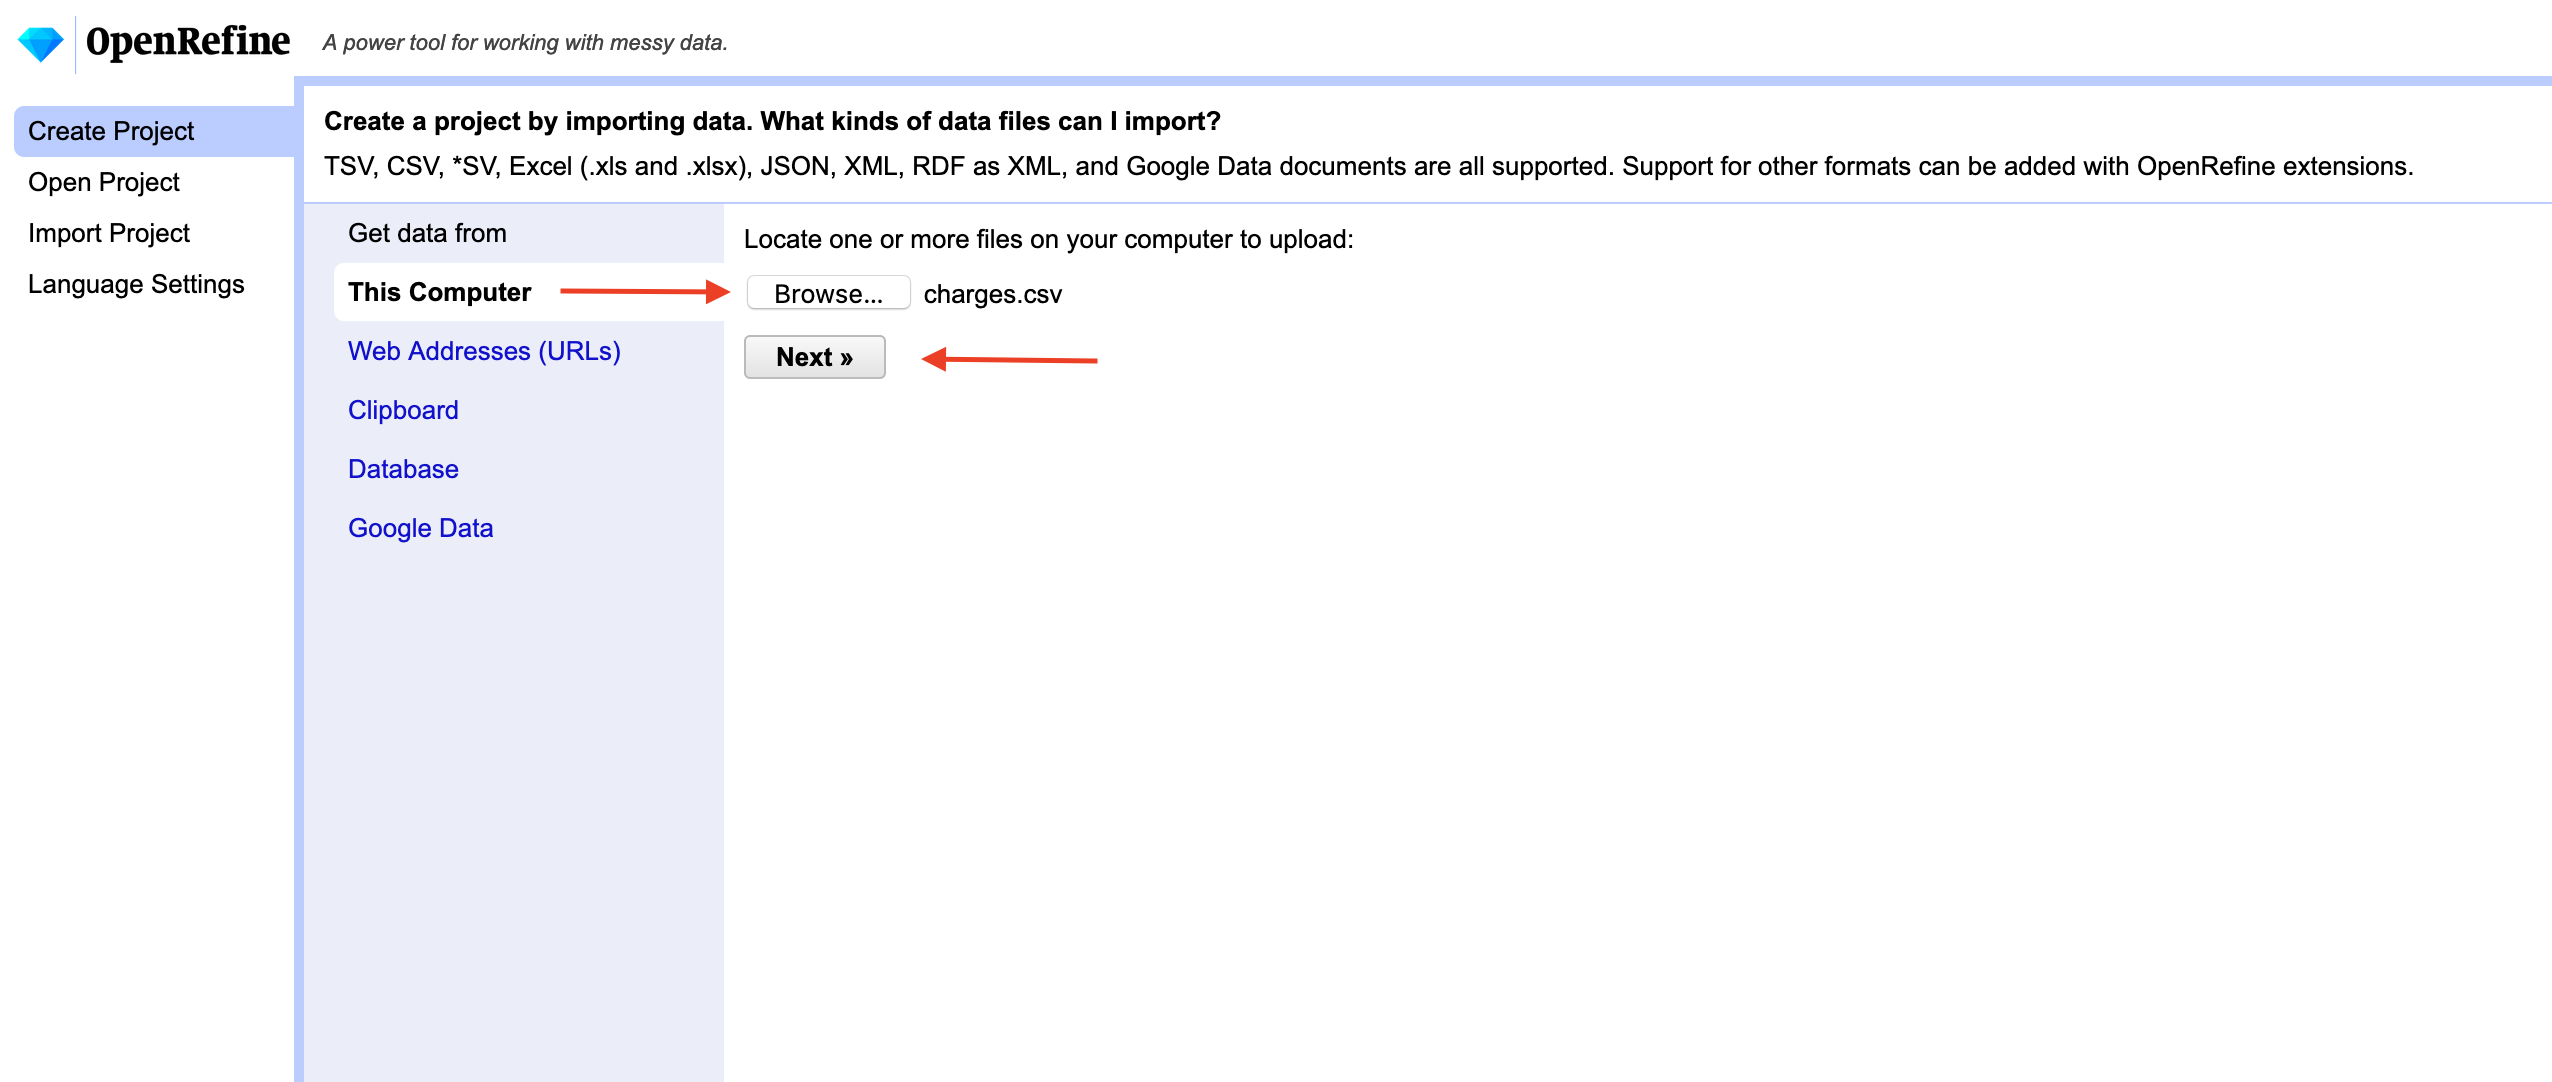
\includegraphics{./images/open1.png}

After your data is loaded into the app, you'll get a screen to look over
what the data looks like. On the top right corner, you'll see a button
to create the project. Click that.

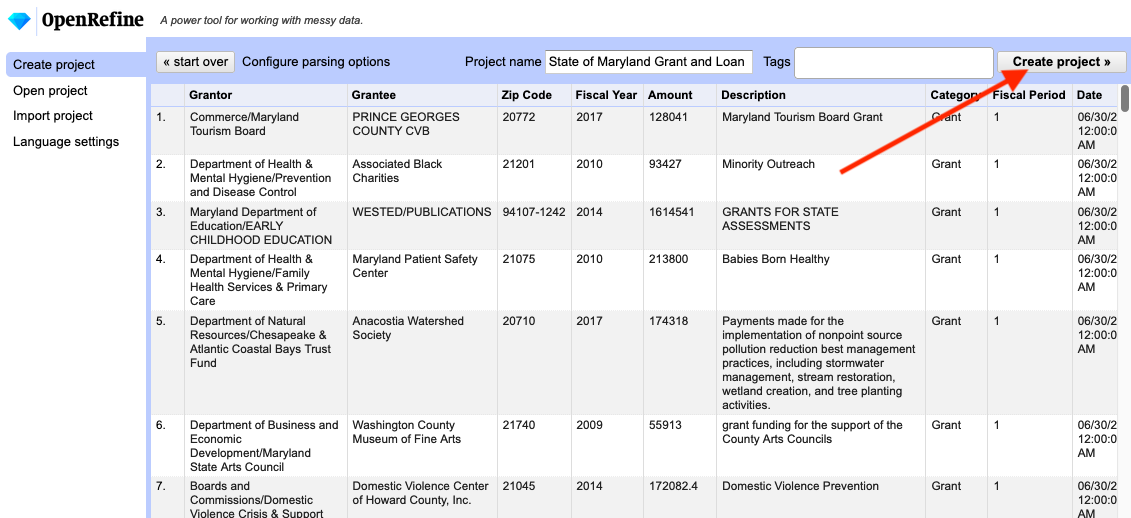
\includegraphics{./images/open2.png}

Open Refine has many, many tools. We're going to use one piece of it, as
a tool for data cleaning. To learn how to use it, we're going to clean
the ``recipient\_name'' field.

First, let's make a copy of the original recipient\_name column so that
we can preserve the original data while cleaning the new one.

Click the dropdown arrow next to the recipient\_name column, choose
``edit column'' \textgreater{} ``Add column based on this column'':

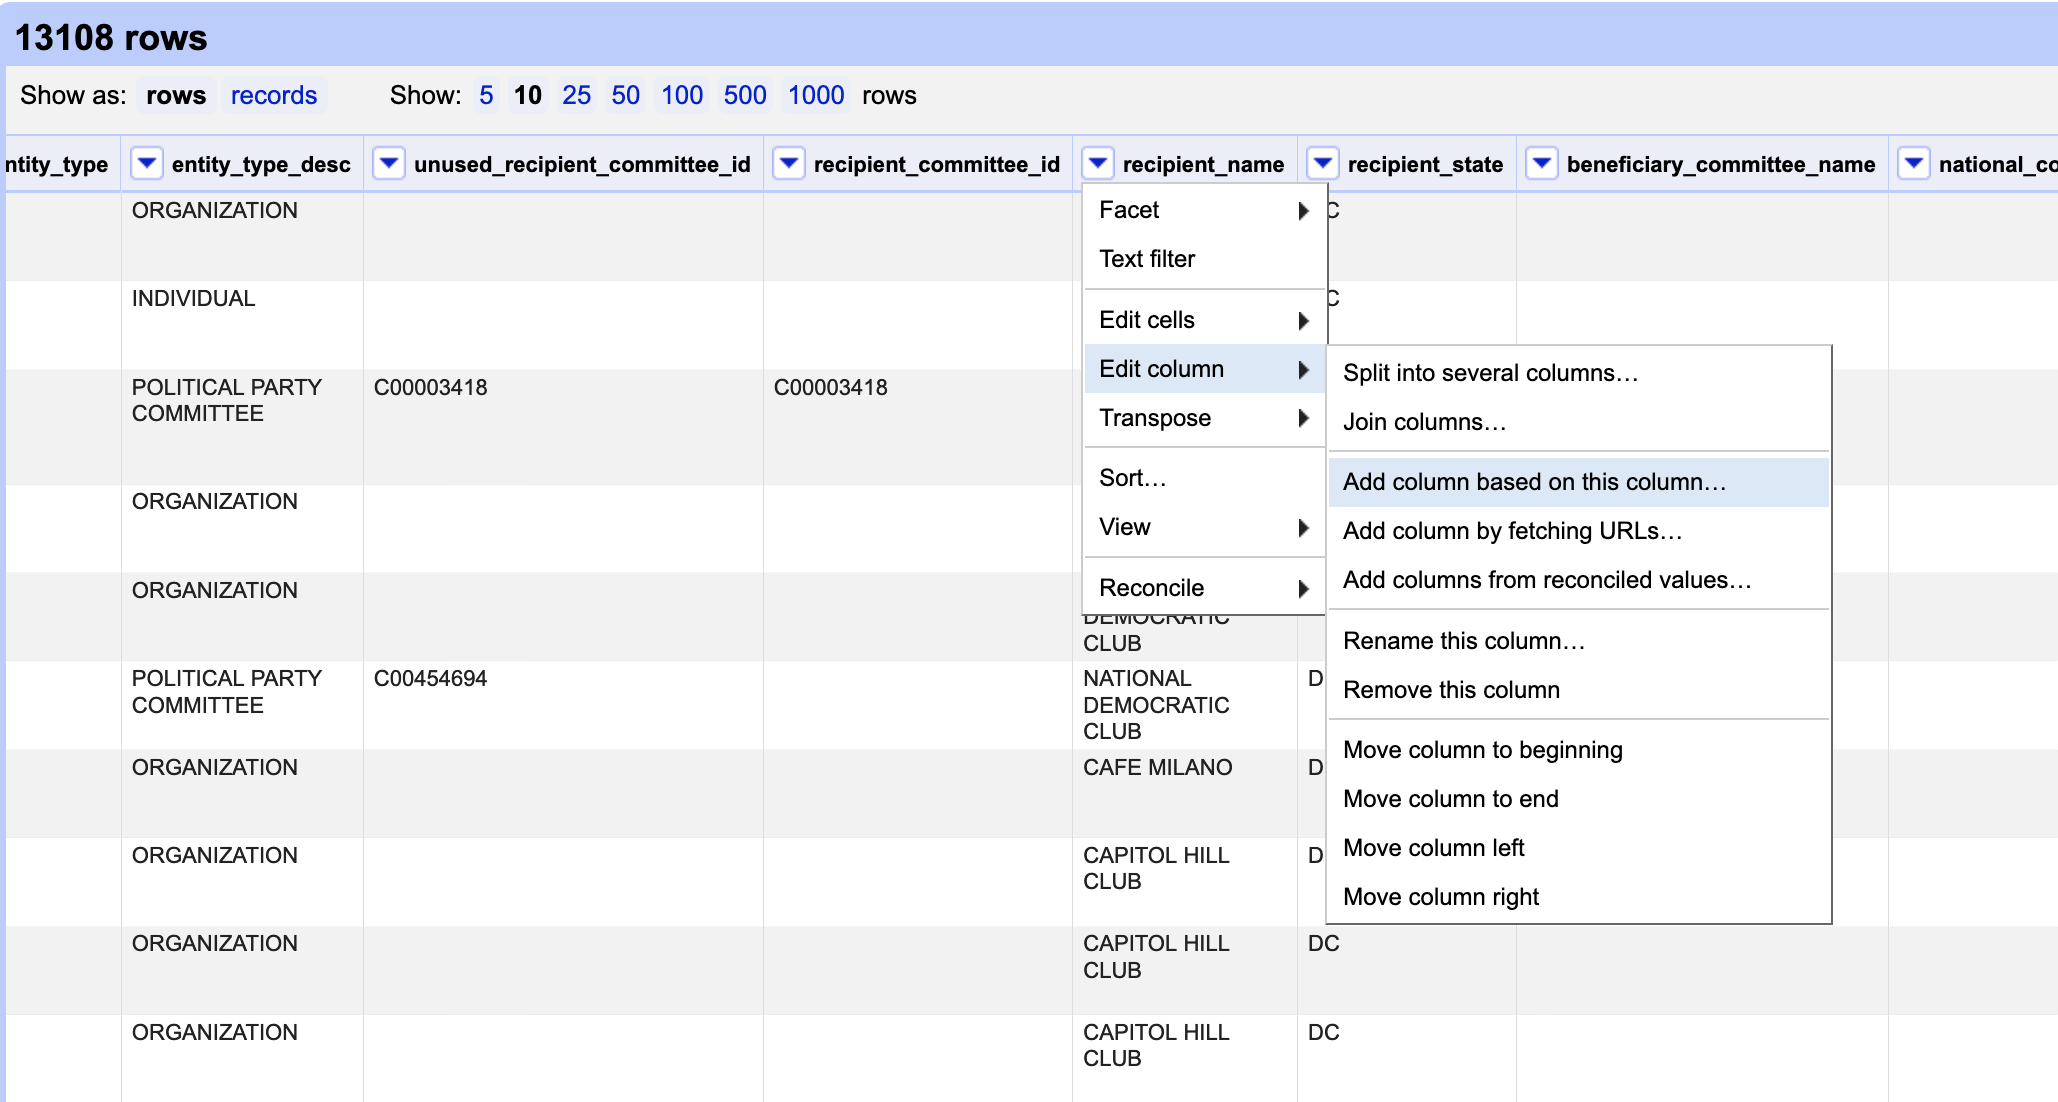
\includegraphics{./images/open2a.png}

On the window that pops up, type ``recipient\_name\_orig'' in the ``new
column name'' field. Then hit the OK button.

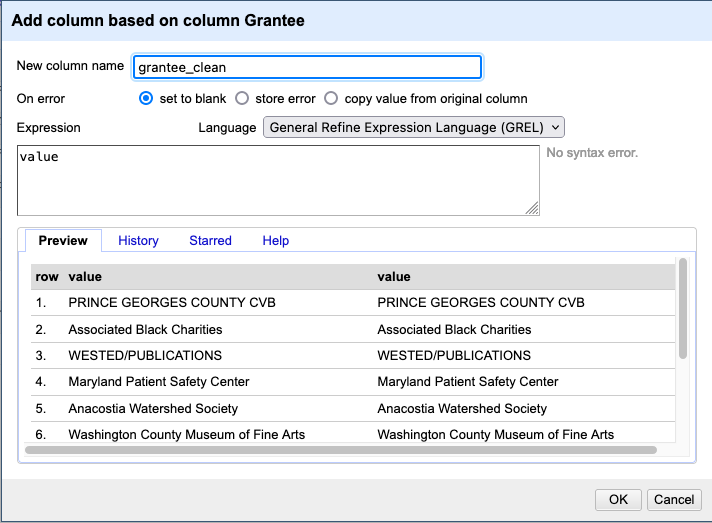
\includegraphics{./images/open2b.png}

Now, let's get to work cleaning the recipient\_name column.

Next to the recipient\_name field name, click the down arrow, then
facet, then text facet.

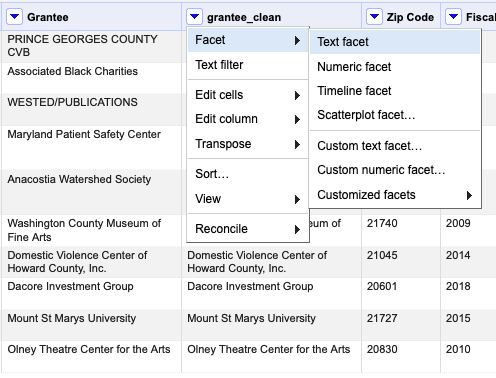
\includegraphics{./images/open3.png}

After that, a new box will appear on the left. It tells us how many
unique recipient\_names there are: 1,655. And, there's a button on the
right of the box that says Cluster.

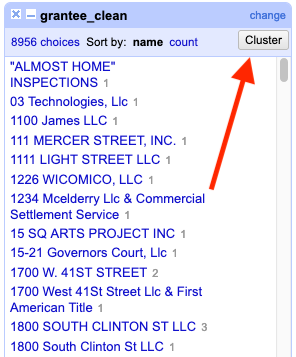
\includegraphics{./images/open4.png}

Click the cluster button. A new window will pop up, a tool to help us
identify things that need to be cleaned, and quickly clean them.

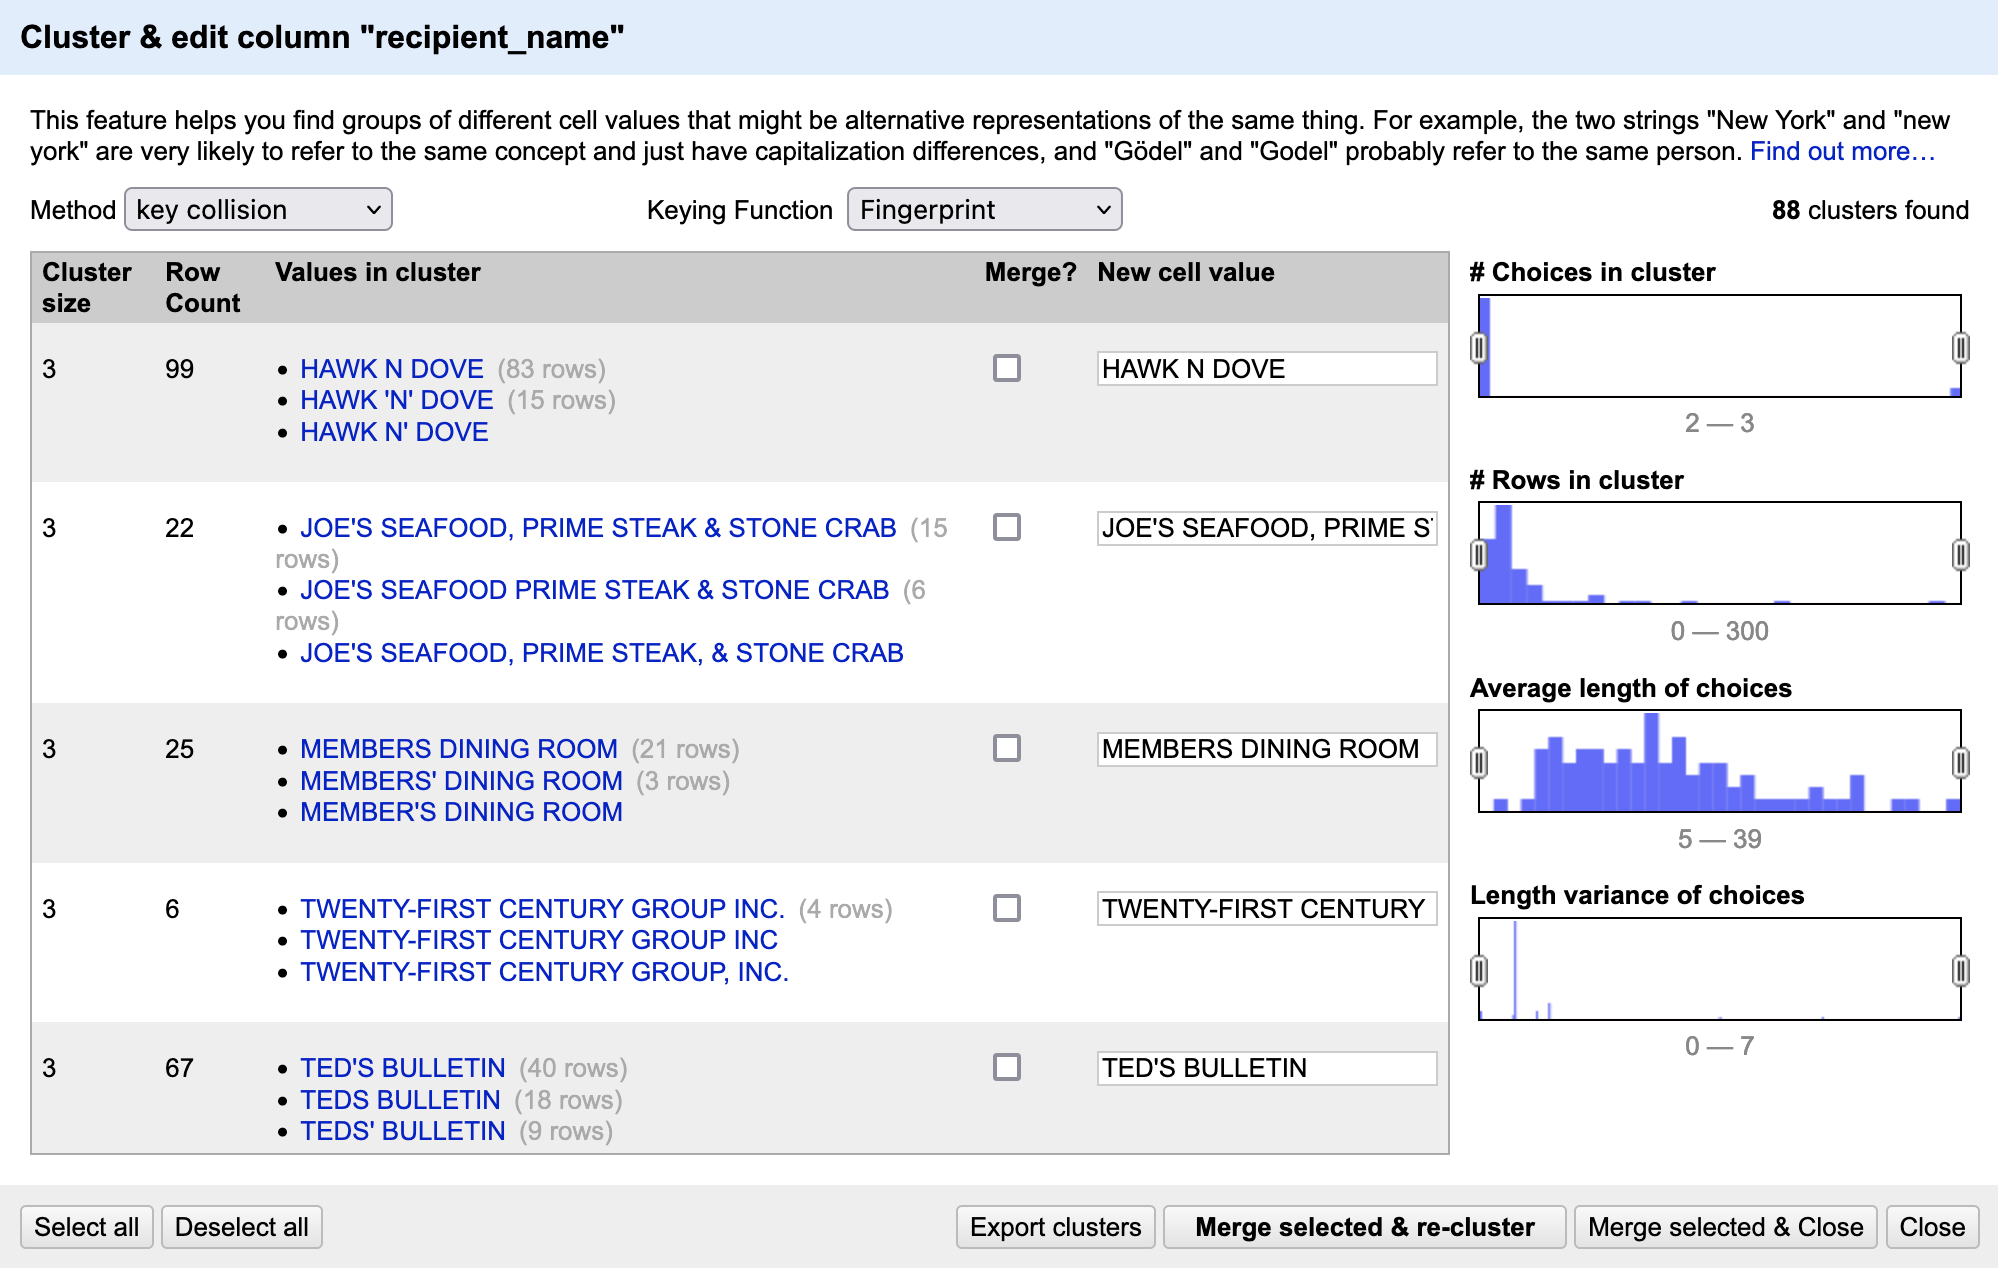
\includegraphics{./images/open5.png}

The default ``method'' used is a clustering algorithim called ``key
collision'', using the fingerprint function. This is the same method we
used with the refinr package above.

At the top, you'll see which method was used, and how many clusters that
algorithm identified. There are several different methods, each of which
work slightly differently and produce different results.

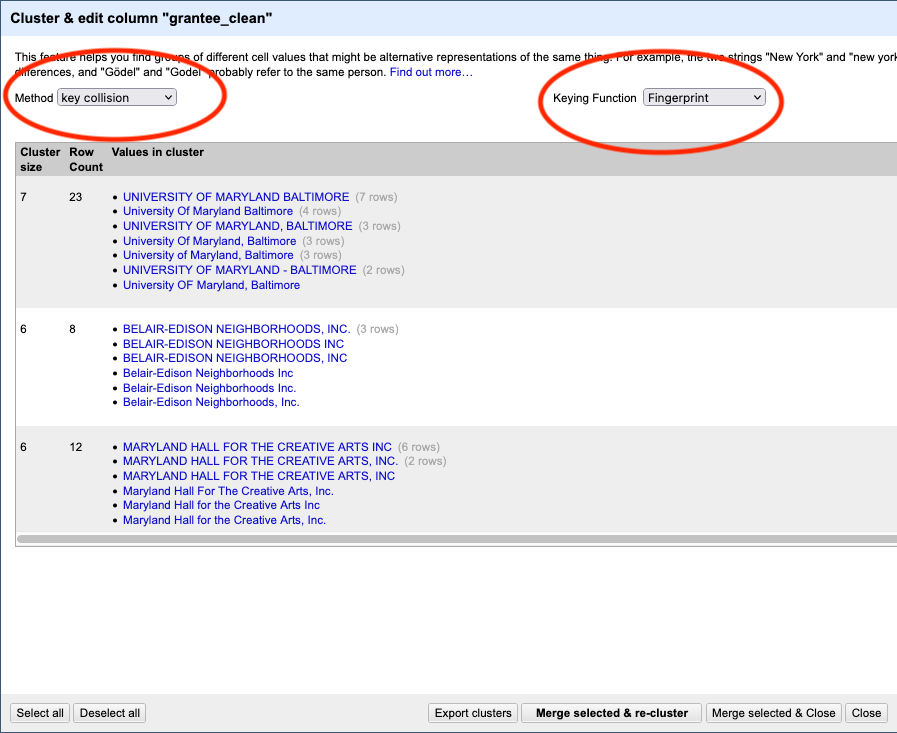
\includegraphics{./images/open6.png}

Then, below that, you can see what those clusters are. Right away, we
can see how useful this program is. It identified 99 rows that have some
variation on ``Hawk N Dove'' in the recipient\_name field. It proposed
changing them all to ``HAWK N DOVE''.

Using human judgement, you can say if you agree with the cluster. If you
do, click the ``merge'' checkbox. When it merges, the new result will be
what it says in New Cell Value. Most often, that's the row with the most
common result. You also can manually edit the ``New Cell Value'' if you
want it to be something else:

Now begins the fun part: You have to look at all 88 clusters found and
decide if they are indeed valid. The key collision method is very good,
and very conservative. You'll find that most of them are usually valid.

Be careful! If you merge two things that aren't supposed to be together,
it will change your data in a way that could lead to inaccurate results.

When you're done, click Merge Selected and Re-Cluster.

If any new clusters come up, evaluate them. Repeat until either no
clusters come up or the clusters that do come up are ones you reject.

Now. Try a new method, maybe the ``nearest neighbor levenshtein''
method. Notice that it finds even more clusters - 167 - using a slightly
different approach.

Rinse and repeat.

You'll keep doing this, and if the dataset is reasonably clean, you'll
find the end.

When you're finished cleaning, click ``Merge Selected \& Close''.

Then, export the data as a csv so you can load it back into R.

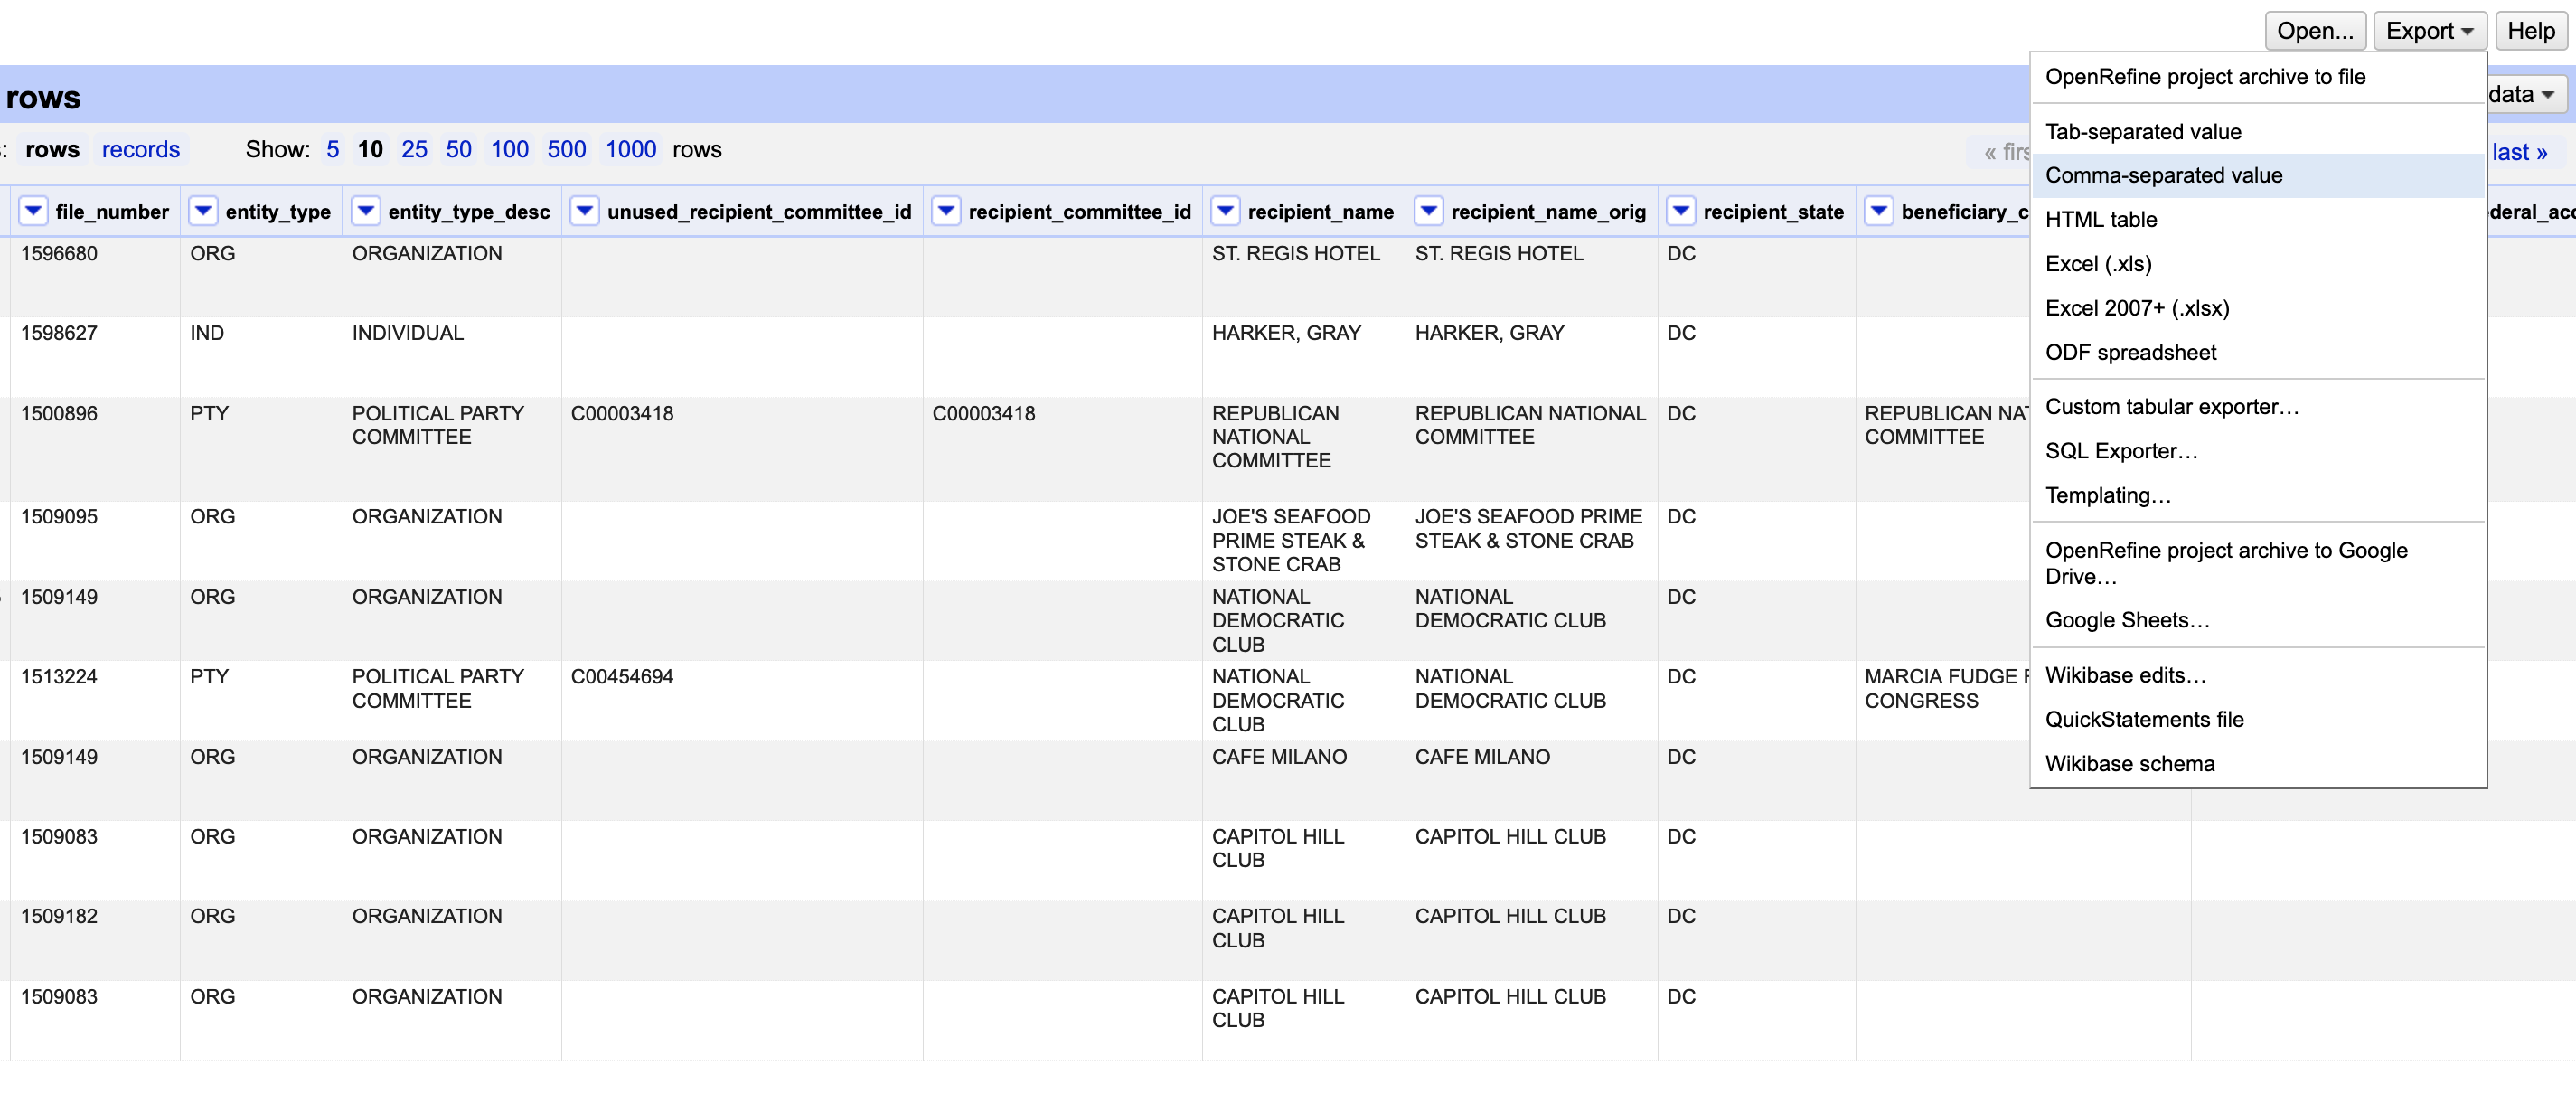
\includegraphics{./images/open7.png}

A question for all data analysts -- if the dataset is bad enough, can it
ever be cleaned?

There's no good answer. You have to find it yourself.

\bookmarksetup{startatroot}

\hypertarget{cleaning-data-part-iv-pdfs}{%
\chapter{Cleaning Data Part IV: PDFs}\label{cleaning-data-part-iv-pdfs}}

The next circle of Hell on the Dante's Inferno of Data Journalism is the
PDF. Governments everywhere love the PDF and publish all kinds of
records in a PDF. The problem is a PDF isn't a data format -- it's a
middle finger, saying I've Got Your Accountability Right Here, Pal.

It's so ridiculous that there's a constellation of tools that do nothing
more than try to harvest tables out of PDFs. There are online services
like \href{https://www.cometdocs.com/}{CometDocs} where you can upload
your PDF and point and click your way into an Excel file. There are
mobile device apps that take a picture of a table and convert it into a
spreadsheet. But one of the best is a tool called
\href{https://tabula.technology/}{Tabula}. It was build by journalists
for journalists.

There is a version of Tabula that will run inside of R -- a library
called Tabulizer -- but the truth is I'm having the hardest time
installing it on my machine, which leads me to believe that trying to
install it across a classroom of various machines would be disastrous.
The standalone version works just fine, and it provides a useful way for
you to see what's actually going on.

Unfortunately, harvesting tables from PDFs with Tabula is an exercise in
getting your hopes up, only to have them dashed. We'll start with an
example. First, let's load the tidyverse and janitor.

\begin{Shaded}
\begin{Highlighting}[]
\FunctionTok{library}\NormalTok{(tidyverse)}
\FunctionTok{library}\NormalTok{(janitor)}
\end{Highlighting}
\end{Shaded}

\hypertarget{easy-does-it}{%
\section{Easy does it}\label{easy-does-it}}

Tabula works best when tables in PDFs are clearly defined and have
nicely-formatted information. Here's a perfect example:
\href{https://elections.maryland.gov/press_room/2020_stats/Eligible\%20Active\%20Voters\%20by\%20County\%20-\%20PG20.pdf}{active
voters by county in Maryland}.

\href{https://tabula.technology/}{Download and install Tabula}. Tabula
works much the same way as Open Refine does -- it works in the browser
by spinning up a small webserver in your computer.

When Tabula opens, you click browse to find the PDF on your computer
somewhere, and then click import. After it imports, click autodetect
tables. You'll see red boxes appear around what Tabula believes are the
tables. You'll see it does a pretty good job at this.

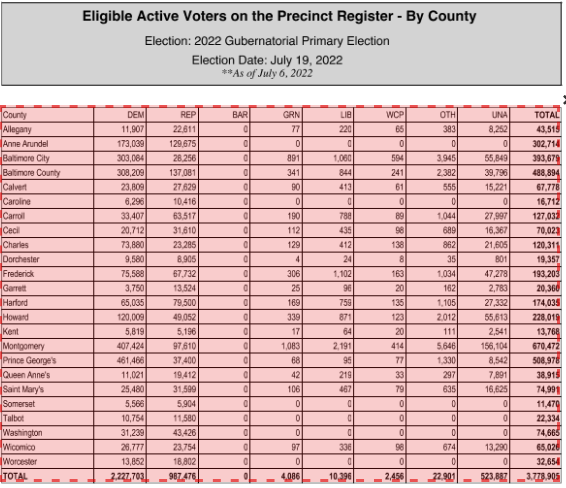
\includegraphics{./images/md_voters.png}

Now you can hit the green ``Preview \& Export Extracted Data'' button on
the top right. You should see something very like this:

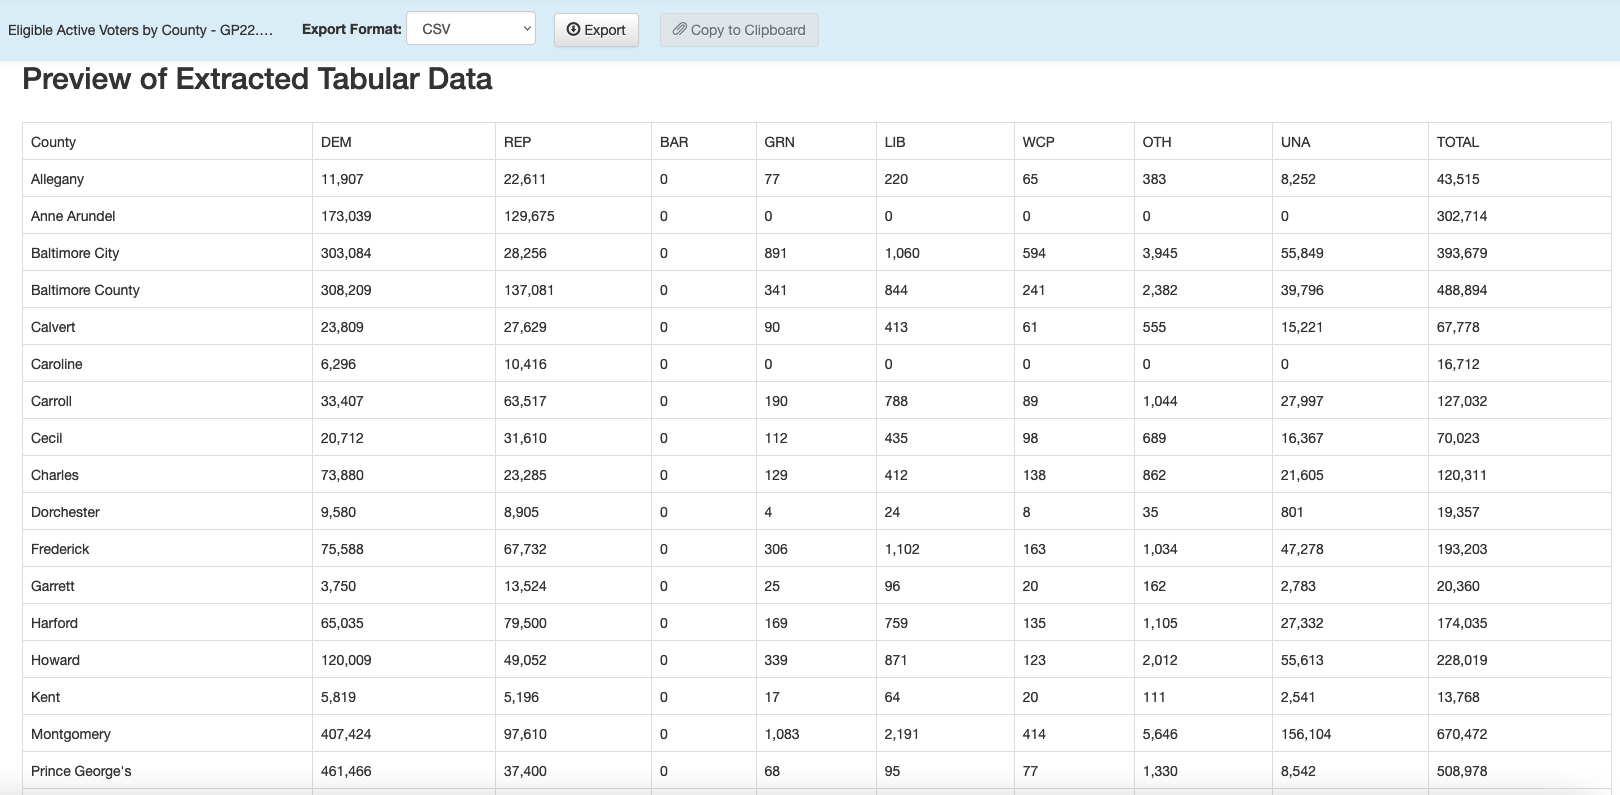
\includegraphics{./images/md_voters2.png}

You can now export that extracted table to a CSV file using the
``Export'' button. And then we can read it into R:

\begin{Shaded}
\begin{Highlighting}[]
\NormalTok{voters\_by\_county }\OtherTok{\textless{}{-}} \FunctionTok{read\_csv}\NormalTok{(}\StringTok{"data/tabula{-}Eligible Active Voters by County {-} PG20.csv"}\NormalTok{)}
\end{Highlighting}
\end{Shaded}

\begin{verbatim}
Rows: 25 Columns: 10
-- Column specification --------------------------------------------------------
Delimiter: ","
chr (1): County

i Use `spec()` to retrieve the full column specification for this data.
i Specify the column types or set `show_col_types = FALSE` to quiet this message.
\end{verbatim}

\begin{Shaded}
\begin{Highlighting}[]
\NormalTok{voters\_by\_county}
\end{Highlighting}
\end{Shaded}

\begin{verbatim}
# A tibble: 25 x 10
   County              DEM    REP   BAR   GRN   LIB   WCP   OTH    UNA  TOTAL
   <chr>             <dbl>  <dbl> <dbl> <dbl> <dbl> <dbl> <dbl>  <dbl>  <dbl>
 1 Allegany          12820  22530    20    74   204    19   395   7674  43736
 2 Anne Arundel     174494 135457   105   564  1922   197  2715  90162 405616
 3 Baltimore City   311610  30163   130   802   951   290  3289  52450 399685
 4 Baltimore County 313870 142534   134   898  2227   297  5872 100576 566408
 5 Calvert           24587  28181    20    89   332    30   567  14178  67984
 6 Caroline           6629  10039     2    33    86    17   163   4208  21177
 7 Carroll           33662  63967    27   155   670    38  1072  25770 125361
 8 Cecil             21601  30880     8   103   341    49   727  15110  68819
 9 Charles           72416  24711    19   112   349    83   763  19849 118302
10 Dorchester         9848   8730     4    19    78    12   148   3348  22187
# ... with 15 more rows
\end{verbatim}

Boom - we're good to go.

\hypertarget{when-it-looks-good-but-needs-a-little-fixing}{%
\section{When it looks good, but needs a little
fixing}\label{when-it-looks-good-but-needs-a-little-fixing}}

Here's a slightly more involved PDF. Here's a
\href{https://raw.githubusercontent.com/openelections/openelections-sources-pa/master/2020/general/Fayette\%20PA\%202020\%20General\%20Summary.pdf}{PDF
of 2020 general election results from Fayette County, Pa.}.

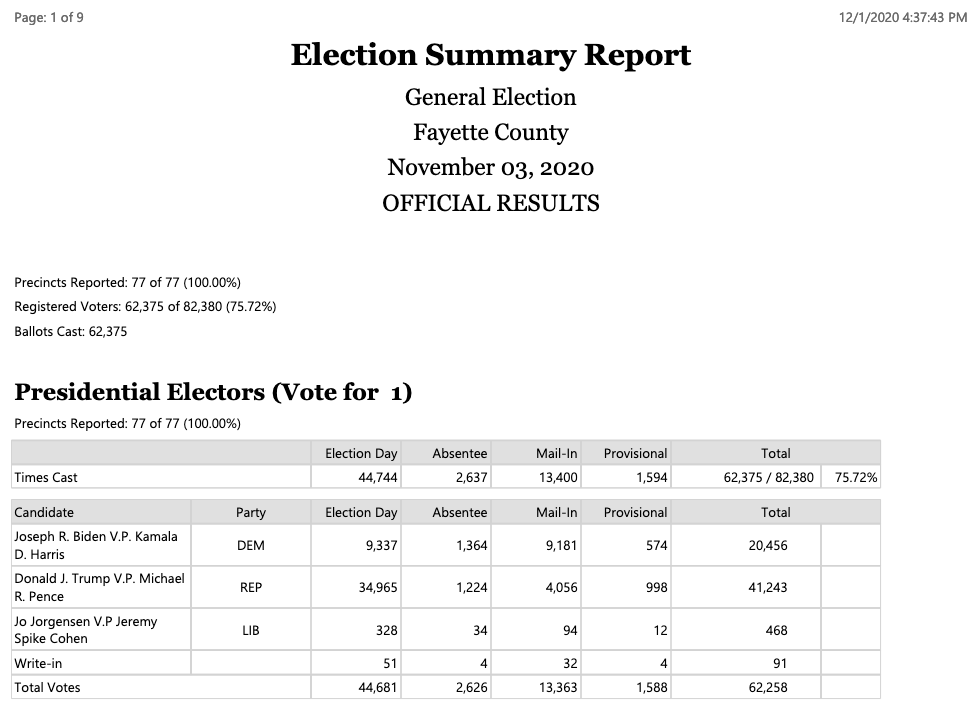
\includegraphics{./images/fayette_1.png}

Looks like a spreadsheet, right? Save that PDF file to your computer in
a place where you'll remember it (like a Downloads folder).

Now let's repeat the steps we did to import the PDF into Tabula and
autodetect the tables. It should look like this:

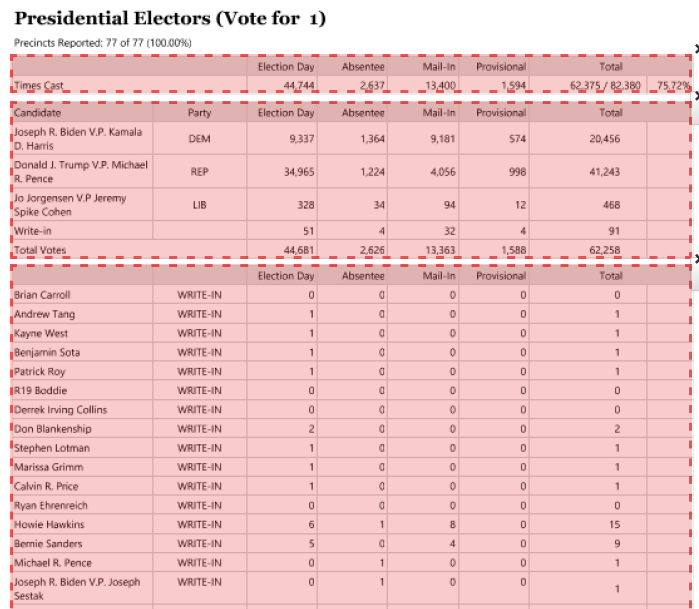
\includegraphics{./images/fayette_2.png}

This is pretty good, but we don't want the ``Times Cast'' boxes at the
top of each contest, because they have a slightly different layout. Go
through the pages (there are 9 of them) and click the ``x'' to the right
of those to clear them.

Now you can hit the green ``Preview \& Export Extracted Data'' button on
the top right. Using the ``Lattice'' method, you should see something
very like this:

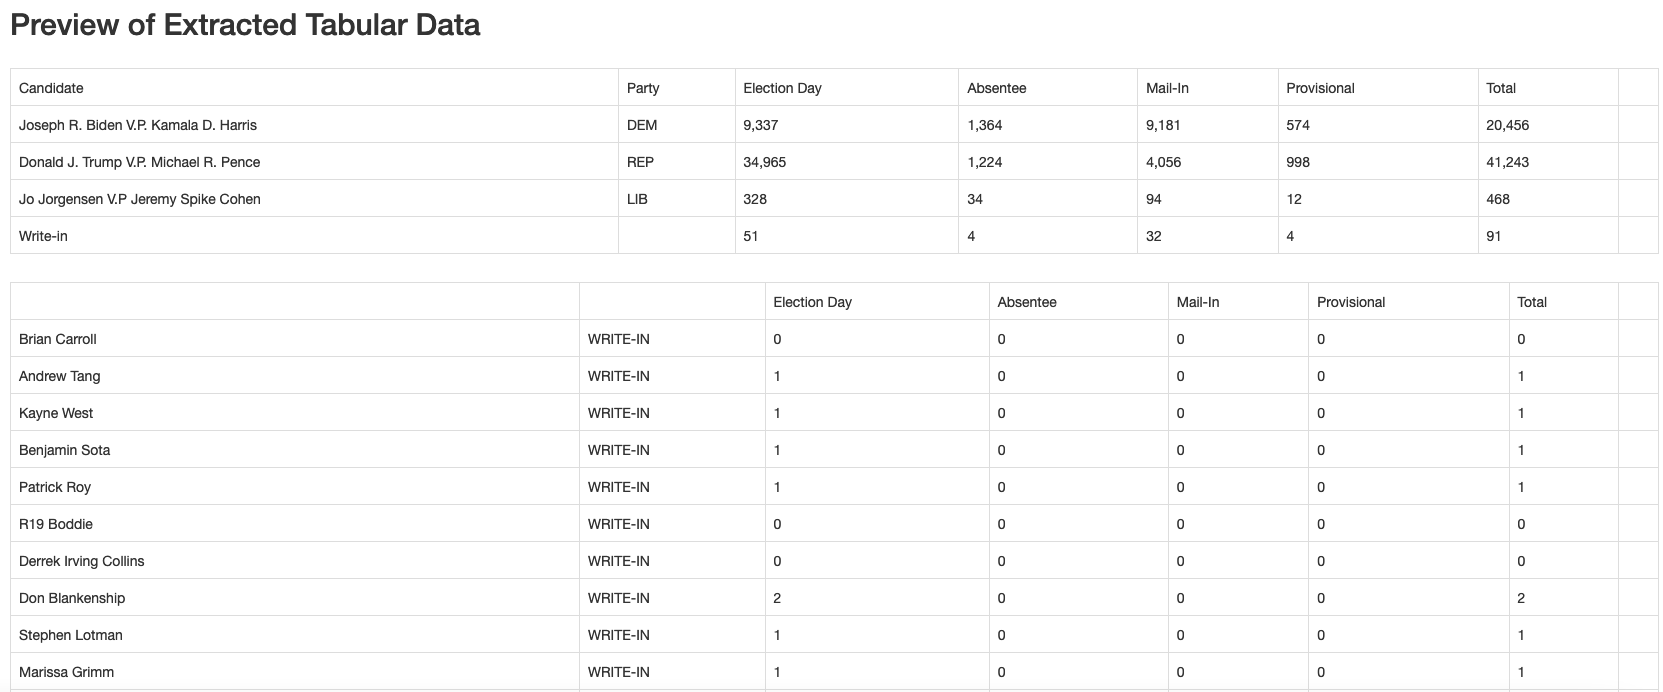
\includegraphics{./images/fayette_3.png}

You can now export that extracted table to a CSV file using the
``Export'' button. And then we can read it into R and clean up the
column names:

\begin{Shaded}
\begin{Highlighting}[]
\NormalTok{fayette\_2020 }\OtherTok{\textless{}{-}} \FunctionTok{read\_csv}\NormalTok{(}\StringTok{"data/tabula{-}Fayette PA 2020 General Summary.csv"}\NormalTok{) }\SpecialCharTok{\%\textgreater{}\%} \FunctionTok{clean\_names}\NormalTok{()}
\end{Highlighting}
\end{Shaded}

\begin{verbatim}
New names:
* `` -> `...8`
\end{verbatim}

\begin{verbatim}
Warning: One or more parsing issues, see `problems()` for details
\end{verbatim}

\begin{verbatim}
Rows: 284 Columns: 8
-- Column specification --------------------------------------------------------
Delimiter: ","
chr (7): Candidate, Party, Election Day, Absentee, Mail-In, Provisional, Total
lgl (1): ...8

i Use `spec()` to retrieve the full column specification for this data.
i Specify the column types or set `show_col_types = FALSE` to quiet this message.
\end{verbatim}

\begin{Shaded}
\begin{Highlighting}[]
\NormalTok{fayette\_2020}
\end{Highlighting}
\end{Shaded}

\begin{verbatim}
# A tibble: 284 x 8
   candidate                   party elect~1 absen~2 mail_in provi~3 total x8   
   <chr>                       <chr> <chr>   <chr>   <chr>   <chr>   <chr> <lgl>
 1 "Joseph R. Biden V.P. Kama~ DEM   9,337   1,364   9,181   574     20,4~ NA   
 2 "Donald J. Trump V.P. Mich~ REP   34,965  1,224   4,056   998     41,2~ NA   
 3 "Jo Jorgensen V.P Jeremy\r~ LIB   328     34      94      12      468   NA   
 4 "Write-in"                  <NA>  51      4       32      4       91    NA   
 5  <NA>                       <NA>  Electi~ Absent~ Mail-In Provis~ Total NA   
 6 "Brian Carroll"             WRIT~ 0       0       0       0       0     NA   
 7 "Andrew Tang"               WRIT~ 1       0       0       0       1     NA   
 8 "Kayne West"                WRIT~ 1       0       0       0       1     NA   
 9 "Benjamin Sota"             WRIT~ 1       0       0       0       1     NA   
10 "Patrick Roy"               WRIT~ 1       0       0       0       1     NA   
# ... with 274 more rows, and abbreviated variable names 1: election_day,
#   2: absentee, 3: provisional
\end{verbatim}

\hypertarget{cleaning-up-the-data-in-r}{%
\section{Cleaning up the data in R}\label{cleaning-up-the-data-in-r}}

The good news is that we have data we don't have to retype. The bad news
is, it's hardly in importable shape. We have a few things to fix. All
the columns with the number of votes in them have commas, which causes R
to think they are columns, not numbers. Let's fix that by re-importing
it and calling \texttt{mutate} so that those columns are numeric.

\begin{Shaded}
\begin{Highlighting}[]
\NormalTok{fayette\_2020 }\OtherTok{\textless{}{-}} \FunctionTok{read\_csv}\NormalTok{(}\StringTok{"data/tabula{-}Fayette PA 2020 General Summary.csv"}\NormalTok{) }\SpecialCharTok{\%\textgreater{}\%} \FunctionTok{clean\_names}\NormalTok{()}
\end{Highlighting}
\end{Shaded}

\begin{verbatim}
New names:
* `` -> `...8`
\end{verbatim}

\begin{verbatim}
Warning: One or more parsing issues, see `problems()` for details
\end{verbatim}

\begin{verbatim}
Rows: 284 Columns: 8
-- Column specification --------------------------------------------------------
Delimiter: ","
chr (7): Candidate, Party, Election Day, Absentee, Mail-In, Provisional, Total
lgl (1): ...8

i Use `spec()` to retrieve the full column specification for this data.
i Specify the column types or set `show_col_types = FALSE` to quiet this message.
\end{verbatim}

\begin{Shaded}
\begin{Highlighting}[]
\NormalTok{fayette\_2020 }\OtherTok{\textless{}{-}}\NormalTok{ fayette\_2020 }\SpecialCharTok{\%\textgreater{}\%} \FunctionTok{mutate}\NormalTok{(}\AttributeTok{election\_day=}\FunctionTok{as.numeric}\NormalTok{(}\FunctionTok{parse\_number}\NormalTok{(election\_day)), }\AttributeTok{absentee=}\FunctionTok{as.numeric}\NormalTok{(}\FunctionTok{parse\_number}\NormalTok{(absentee)), }\AttributeTok{mail\_in=}\FunctionTok{as.numeric}\NormalTok{(}\FunctionTok{parse\_number}\NormalTok{(mail\_in)), }\AttributeTok{provisional=}\FunctionTok{as.numeric}\NormalTok{(}\FunctionTok{parse\_number}\NormalTok{(provisional)),}\AttributeTok{total=}\FunctionTok{as.numeric}\NormalTok{(}\FunctionTok{parse\_number}\NormalTok{(total)))}
\end{Highlighting}
\end{Shaded}

\begin{verbatim}
Warning: 20 parsing failures.
row col expected       actual
  5  -- a number Election Day
 25  -- a number Election Day
 73  -- a number Election Day
 74  -- a number Election Day
 80  -- a number Election Day
... ... ........ ............
See problems(...) for more details.
\end{verbatim}

\begin{verbatim}
Warning: 20 parsing failures.
row col expected   actual
  5  -- a number Absentee
 25  -- a number Absentee
 73  -- a number Absentee
 74  -- a number Absentee
 80  -- a number Absentee
... ... ........ ........
See problems(...) for more details.
\end{verbatim}

\begin{verbatim}
Warning: 20 parsing failures.
row col expected  actual
  5  -- a number Mail-In
 25  -- a number Mail-In
 73  -- a number Mail-In
 74  -- a number Mail-In
 80  -- a number Mail-In
... ... ........ .......
See problems(...) for more details.
\end{verbatim}

\begin{verbatim}
Warning: 20 parsing failures.
row col expected      actual
  5  -- a number Provisional
 25  -- a number Provisional
 73  -- a number Provisional
 74  -- a number Provisional
 80  -- a number Provisional
... ... ........ ...........
See problems(...) for more details.
\end{verbatim}

\begin{verbatim}
Warning: 20 parsing failures.
row col expected actual
  5  -- a number  Total
 25  -- a number  Total
 73  -- a number  Total
 74  -- a number  Total
 80  -- a number  Total
... ... ........ ......
See problems(...) for more details.
\end{verbatim}

\begin{Shaded}
\begin{Highlighting}[]
\NormalTok{fayette\_2020}
\end{Highlighting}
\end{Shaded}

\begin{verbatim}
# A tibble: 284 x 8
   candidate                   party elect~1 absen~2 mail_in provi~3 total x8   
   <chr>                       <chr>   <dbl>   <dbl>   <dbl>   <dbl> <dbl> <lgl>
 1 "Joseph R. Biden V.P. Kama~ DEM      9337    1364    9181     574 20456 NA   
 2 "Donald J. Trump V.P. Mich~ REP     34965    1224    4056     998 41243 NA   
 3 "Jo Jorgensen V.P Jeremy\r~ LIB       328      34      94      12   468 NA   
 4 "Write-in"                  <NA>       51       4      32       4    91 NA   
 5  <NA>                       <NA>       NA      NA      NA      NA    NA NA   
 6 "Brian Carroll"             WRIT~       0       0       0       0     0 NA   
 7 "Andrew Tang"               WRIT~       1       0       0       0     1 NA   
 8 "Kayne West"                WRIT~       1       0       0       0     1 NA   
 9 "Benjamin Sota"             WRIT~       1       0       0       0     1 NA   
10 "Patrick Roy"               WRIT~       1       0       0       0     1 NA   
# ... with 274 more rows, and abbreviated variable names 1: election_day,
#   2: absentee, 3: provisional
\end{verbatim}

Ok, now we have numbers. Next we'll get rid of the rows where
\texttt{candidate} is NA or the value of \texttt{candidate} is literally
``Candidate'' and also drop the \texttt{x8} blank column. To do the
former, we'll use the inverse of the \texttt{is.na} function by placing
an exclamation point before it (you can read that filter as ``where
candidate is NOT NA'') and do the same to exclude ``Candidate'' from the
matching values. For the latter, we'll use select and the minus sign to
drop that column

\begin{Shaded}
\begin{Highlighting}[]
\NormalTok{fayette\_2020 }\OtherTok{\textless{}{-}}\NormalTok{ fayette\_2020 }\SpecialCharTok{\%\textgreater{}\%} \FunctionTok{filter}\NormalTok{(}\SpecialCharTok{!}\FunctionTok{is.na}\NormalTok{(candidate)) }\SpecialCharTok{\%\textgreater{}\%} \FunctionTok{filter}\NormalTok{(candidate }\SpecialCharTok{!=} \StringTok{"Candidate"}\NormalTok{) }\SpecialCharTok{\%\textgreater{}\%} \FunctionTok{select}\NormalTok{(}\SpecialCharTok{{-}}\NormalTok{x8)}

\NormalTok{fayette\_2020}
\end{Highlighting}
\end{Shaded}

\begin{verbatim}
# A tibble: 264 x 7
   candidate                         party elect~1 absen~2 mail_in provi~3 total
   <chr>                             <chr>   <dbl>   <dbl>   <dbl>   <dbl> <dbl>
 1 "Joseph R. Biden V.P. Kamala\rD.~ DEM      9337    1364    9181     574 20456
 2 "Donald J. Trump V.P. Michael\rR~ REP     34965    1224    4056     998 41243
 3 "Jo Jorgensen V.P Jeremy\rSpike ~ LIB       328      34      94      12   468
 4 "Write-in"                        <NA>       51       4      32       4    91
 5 "Brian Carroll"                   WRIT~       0       0       0       0     0
 6 "Andrew Tang"                     WRIT~       1       0       0       0     1
 7 "Kayne West"                      WRIT~       1       0       0       0     1
 8 "Benjamin Sota"                   WRIT~       1       0       0       0     1
 9 "Patrick Roy"                     WRIT~       1       0       0       0     1
10 "R19 Boddie"                      WRIT~       0       0       0       0     0
# ... with 254 more rows, and abbreviated variable names 1: election_day,
#   2: absentee, 3: provisional
\end{verbatim}

This still isn't perfect - we don't have the offices these folks are
running for - but all things considered, that was pretty easy. Many -
most? - electronic PDFs aren't so easy to parse. Sometimes you'll need
to open the exported CSV file and clean things up before importing into
R. Other times you'll be able to do that cleaning in R itself.

Here's the sad truth: THIS IS PRETTY GOOD. It sure beats typing it out.
And since many government processes don't change all that much, you can
save the code to process subsequent versions of PDFs.

\bookmarksetup{startatroot}

\hypertarget{combining-and-joining}{%
\chapter{Combining and joining}\label{combining-and-joining}}

Often, as data journalists, we're looking at data across time or at data
stored in multiple tables. And to do that, we need to often need to
merge that data together.

Depending on what we have, we may just need to stack data on top of each
other to make new data. If we have 2019 data and 2018 data and we want
that to be one file, we stack them. If we have a dataset of cows in
counties and a dataset of populations in county, we're going to join
those two together on the county -- the common element.

Let's explore.

\hypertarget{combining-data-stacking}{%
\section{Combining data (stacking)}\label{combining-data-stacking}}

Let's say that we have Maryland county voter registration data from
three different elections in three different files. They have the same
record layout and the same number of counties (plus Baltimore City). We
can combine them into a single dataframe.

Let's do what we need to import them properly. I've merged it all into
one step for each of the three datasets.

\begin{Shaded}
\begin{Highlighting}[]
\FunctionTok{library}\NormalTok{(tidyverse)}
\end{Highlighting}
\end{Shaded}

\begin{Shaded}
\begin{Highlighting}[]
\NormalTok{county\_voters\_2016 }\OtherTok{\textless{}{-}} \FunctionTok{read\_csv}\NormalTok{(}\StringTok{"data/county\_voters\_2016.csv"}\NormalTok{)}
\end{Highlighting}
\end{Shaded}

\begin{verbatim}
Rows: 25 Columns: 9
-- Column specification --------------------------------------------------------
Delimiter: ","
chr (1): COUNTY
dbl (8): YEAR, DEM, REP, LIB, GRN, UNA, OTH, Total

i Use `spec()` to retrieve the full column specification for this data.
i Specify the column types or set `show_col_types = FALSE` to quiet this message.
\end{verbatim}

\begin{Shaded}
\begin{Highlighting}[]
\NormalTok{county\_voters\_2018 }\OtherTok{\textless{}{-}} \FunctionTok{read\_csv}\NormalTok{(}\StringTok{"data/county\_voters\_2018.csv"}\NormalTok{)}
\end{Highlighting}
\end{Shaded}

\begin{verbatim}
Rows: 25 Columns: 9
-- Column specification --------------------------------------------------------
Delimiter: ","
chr (1): COUNTY
dbl (8): YEAR, DEM, REP, LIB, GRN, UNA, OTH, Total

i Use `spec()` to retrieve the full column specification for this data.
i Specify the column types or set `show_col_types = FALSE` to quiet this message.
\end{verbatim}

\begin{Shaded}
\begin{Highlighting}[]
\NormalTok{county\_voters\_2020 }\OtherTok{\textless{}{-}} \FunctionTok{read\_csv}\NormalTok{(}\StringTok{"data/county\_voters\_2020.csv"}\NormalTok{)}
\end{Highlighting}
\end{Shaded}

\begin{verbatim}
Rows: 25 Columns: 9
-- Column specification --------------------------------------------------------
Delimiter: ","
chr (1): COUNTY
dbl (8): YEAR, DEM, REP, GRN, LIB, OTH, UNA, Total

i Use `spec()` to retrieve the full column specification for this data.
i Specify the column types or set `show_col_types = FALSE` to quiet this message.
\end{verbatim}

All three of these datasets have the same number of columns, all with
the same names, so if we want to merge them together to compare them
over time, we need to stack them together. The verb here, in R, is
\texttt{bind\_rows}. You tell the function what you want to combine and
it does it, assuming that you've got column names in common containing
identically formatted data.

Since we have three dataframes, we're going to need to pass them as a
list, meaning they'll be enclosed inside the \texttt{list} function.

\begin{Shaded}
\begin{Highlighting}[]
\NormalTok{county\_voters\_combined }\OtherTok{\textless{}{-}} \FunctionTok{bind\_rows}\NormalTok{(}\FunctionTok{list}\NormalTok{(county\_voters\_2016, county\_voters\_2018, county\_voters\_2020))}
\end{Highlighting}
\end{Shaded}

And boom, like that, we have 75 rows of data together instead of three
dataframes. There are plenty of uses for \texttt{bind\_rows}: any
regularly updated data that comes in the same format like crime reports
or award recipients or player game statistics. Or election results.

\hypertarget{joining-data}{%
\section{Joining data}\label{joining-data}}

More complicated is when you have two separate tables that are connected
by a common element or elements. But there's a verb for that, too:
\texttt{join}.

Let's start by reading in some Maryland 2020 county population data:

\begin{Shaded}
\begin{Highlighting}[]
\NormalTok{maryland\_population }\OtherTok{\textless{}{-}} \FunctionTok{read\_csv}\NormalTok{(}\StringTok{\textquotesingle{}data/maryland\_population\_2020.csv\textquotesingle{}}\NormalTok{)}
\end{Highlighting}
\end{Shaded}

\begin{verbatim}
Rows: 24 Columns: 2
-- Column specification --------------------------------------------------------
Delimiter: ","
chr (1): COUNTY
dbl (1): POP2020

i Use `spec()` to retrieve the full column specification for this data.
i Specify the column types or set `show_col_types = FALSE` to quiet this message.
\end{verbatim}

One of the columns we have is called \texttt{county}, which is what we
have in our county\_voters\_2020 dataframe.

To put the Maryland population data and voter registration data
together, we need to use something called a join. There are different
kinds of joins. It's better if you think of two tables sitting next to
each other. A \texttt{left\_join} takes all the records from the left
table and only the records that match in the right one. A
\texttt{right\_join} does the same thing. An \texttt{inner\_join} takes
only the records where they are equal. There's one other join -- a
\texttt{full\_join} which returns all rows of both, regardless of if
there's a match -- but I've never once had a use for a full join.

In the best-case scenario, the two tables we want to join share a common
column. In this case, both of our tables have a column called
\texttt{county} that has the same characteristics: values in both look
identical, including how they distinguish Baltimore City from Baltimore
County. This is important, because joins work on \emph{exact matches}.

We can do this join multiple ways and get a similar result. We can put
the population file on the left and the registration data on the right
and use a left join to get them all together. And we use \texttt{by=} to
join by the correct column. I'm going to count the rows at the end. The
reason I'm doing this is important: \textbf{Rule 1 in joining data is
having an idea of what you are expecting to get}. So with a left join
with population on the left, I have 24 rows, so I expect to get 24 rows
when I'm done.

\begin{Shaded}
\begin{Highlighting}[]
\NormalTok{maryland\_population }\SpecialCharTok{\%\textgreater{}\%} \FunctionTok{left\_join}\NormalTok{(county\_voters\_2020, }\AttributeTok{by=}\StringTok{"COUNTY"}\NormalTok{) }\SpecialCharTok{\%\textgreater{}\%} \FunctionTok{nrow}\NormalTok{()}
\end{Highlighting}
\end{Shaded}

\begin{verbatim}
[1] 24
\end{verbatim}

Remove the nrow and run it again for yourself. By default,
\texttt{dplyr} will do a ``natural'' join, where it'll match all the
matching columns in both tables. So if we take out the by, it'll use all
the common columns between the tables. That may not be right in every
instance but let's try it. If it works, we should get 24 rows.

\begin{Shaded}
\begin{Highlighting}[]
\NormalTok{maryland\_population }\SpecialCharTok{\%\textgreater{}\%} \FunctionTok{left\_join}\NormalTok{(county\_voters\_2020)}
\end{Highlighting}
\end{Shaded}

\begin{verbatim}
Joining, by = "COUNTY"
\end{verbatim}

\begin{verbatim}
# A tibble: 24 x 10
   COUNTY           POP2020  YEAR    DEM    REP   GRN   LIB   OTH    UNA  Total
   <chr>              <dbl> <dbl>  <dbl>  <dbl> <dbl> <dbl> <dbl>  <dbl>  <dbl>
 1 Allegany           68106  2020  12820  22530    74   204   434   7674  43736
 2 Anne Arundel      588261  2020 174494 135457   564  1922  3017  90162 405616
 3 Baltimore City    585708  2020 311610  30163   802   951  3709  52450 399685
 4 Baltimore County  854535  2020 313870 142534   898  2227  6303 100576 566408
 5 Calvert            92783  2020  24587  28181    89   332   617  14178  67984
 6 Caroline           33293  2020   6629  10039    33    86   182   4208  21177
 7 Carroll           172891  2020  33662  63967   155   670  1137  25770 125361
 8 Cecil             103725  2020  21601  30880   103   341   784  15110  68819
 9 Charles           166617  2020  72416  24711   112   349   865  19849 118302
10 Dorchester         32531  2020   9848   8730    19    78   164   3348  22187
# ... with 14 more rows
\end{verbatim}

Since we only have one column in common between the two tables, the join
only used that column. And we got the same answer. If we had more
columns in common, you could see in your results columns with .X after
them - that's a sign of duplicative columns between two tables, and you
may decide you don't need both moving forward.

Let's save our joined data to a new dataframe, but this time let's
remove the select function so we don't limit the columns to just three.

\begin{Shaded}
\begin{Highlighting}[]
\NormalTok{maryland\_population\_with\_voters }\OtherTok{\textless{}{-}}\NormalTok{ maryland\_population }\SpecialCharTok{\%\textgreater{}\%} \FunctionTok{left\_join}\NormalTok{(county\_voters\_2020)}
\end{Highlighting}
\end{Shaded}

\begin{verbatim}
Joining, by = "COUNTY"
\end{verbatim}

Now, with our joined data, we can answer questions in a more useful way.
But joins can do even more than just bring data together; they can
include additional data to enable you to ask more sophisticated
questions. Right now we have registered voters and total population. But
we can do more.

Let's try adding more Maryland demographic data to the mix. Using a file
describing the 18-and-over population (from which eligible voters come)
from
\href{https://planning.maryland.gov/MSDC/Pages/census/Census2020/pL_2020redistricting.aspx}{the
state's data catalog}, we can read it into R:

\begin{Shaded}
\begin{Highlighting}[]
\NormalTok{maryland\_demographics }\OtherTok{\textless{}{-}} \FunctionTok{read\_csv}\NormalTok{(}\StringTok{\textquotesingle{}data/maryland\_demographics.csv\textquotesingle{}}\NormalTok{)}
\end{Highlighting}
\end{Shaded}

\begin{verbatim}
Rows: 24 Columns: 11
-- Column specification --------------------------------------------------------
Delimiter: ","
chr  (1): NAME
dbl (10): GEOCODE, pop_18_over, pop_one_race, pop_white, pop_black, pop_nati...

i Use `spec()` to retrieve the full column specification for this data.
i Specify the column types or set `show_col_types = FALSE` to quiet this message.
\end{verbatim}

Again, we can use a \texttt{left\_join} to make our demographic data
available. This time we'll need to specify the two fields to join
because they do not have identical names. We'll use \texttt{COUNTY} from
our population data and \texttt{NAME} from the demographic data, and the
order matters - the first column is from the dataframe you name
\emph{first}.

\begin{Shaded}
\begin{Highlighting}[]
\NormalTok{maryland\_population\_with\_voters\_and\_demographics }\OtherTok{\textless{}{-}}\NormalTok{ maryland\_population\_with\_voters }\SpecialCharTok{\%\textgreater{}\%} \FunctionTok{left\_join}\NormalTok{(maryland\_demographics, }\AttributeTok{by=}\FunctionTok{c}\NormalTok{(}\StringTok{"COUNTY"}\OtherTok{=}\StringTok{"NAME"}\NormalTok{))}
\end{Highlighting}
\end{Shaded}

Now we've got population data and demographic data by county. That means
we can draw from both datasets in asking our questions. For example, we
could see the counties with the highest 18+ Black population as a
percentage of all population 18 and over and also the percentage of
Democrats in that county.

We can get this by using mutate and arrange:

\begin{Shaded}
\begin{Highlighting}[]
\NormalTok{maryland\_population\_with\_voters\_and\_demographics }\SpecialCharTok{\%\textgreater{}\%}
  \FunctionTok{mutate}\NormalTok{(}\AttributeTok{pct\_black\_18\_plus =}\NormalTok{ (pop\_black}\SpecialCharTok{/}\NormalTok{pop\_18\_over)}\SpecialCharTok{*}\DecValTok{100}\NormalTok{, }\AttributeTok{pct\_dems =}\NormalTok{ (DEM}\SpecialCharTok{/}\NormalTok{Total)}\SpecialCharTok{*}\DecValTok{100}\NormalTok{) }\SpecialCharTok{\%\textgreater{}\%}
  \FunctionTok{arrange}\NormalTok{(}\FunctionTok{desc}\NormalTok{(pct\_black\_18\_plus)) }\SpecialCharTok{\%\textgreater{}\%}
  \FunctionTok{select}\NormalTok{(COUNTY, pct\_black\_18\_plus, pct\_dems)}
\end{Highlighting}
\end{Shaded}

\begin{verbatim}
# A tibble: 24 x 3
   COUNTY           pct_black_18_plus pct_dems
   <chr>                        <dbl>    <dbl>
 1 Prince George's               60.9     78.3
 2 Baltimore City                56.3     78.0
 3 Charles                       48.2     61.2
 4 Somerset                      39.0     41.8
 5 Baltimore County              28.8     55.4
 6 Dorchester                    26.2     44.4
 7 Wicomico                      25.6     42.3
 8 Howard                        18.7     52.4
 9 Montgomery                    18.1     61.0
10 Anne Arundel                  17.4     43.0
# ... with 14 more rows
\end{verbatim}

If you know Maryland political demographics, this result isn't too
surprising, but Somerset County - the state's 2nd smallest in terms of
population - stands out for its Black population, which is a greater
percentage than Baltimore County and Montgomery County.

Let's change that to look at Asian population:

\begin{Shaded}
\begin{Highlighting}[]
\NormalTok{maryland\_population\_with\_voters\_and\_demographics }\SpecialCharTok{\%\textgreater{}\%}
  \FunctionTok{mutate}\NormalTok{(}\AttributeTok{pct\_asian\_18\_plus =}\NormalTok{ (pop\_asian}\SpecialCharTok{/}\NormalTok{pop\_18\_over)}\SpecialCharTok{*}\DecValTok{100}\NormalTok{, }\AttributeTok{pct\_dems =}\NormalTok{ (DEM}\SpecialCharTok{/}\NormalTok{Total)}\SpecialCharTok{*}\DecValTok{100}\NormalTok{) }\SpecialCharTok{\%\textgreater{}\%}
  \FunctionTok{arrange}\NormalTok{(}\FunctionTok{desc}\NormalTok{(pct\_asian\_18\_plus)) }\SpecialCharTok{\%\textgreater{}\%}
  \FunctionTok{select}\NormalTok{(COUNTY, pct\_asian\_18\_plus, pct\_dems)}
\end{Highlighting}
\end{Shaded}

\begin{verbatim}
# A tibble: 24 x 3
   COUNTY           pct_asian_18_plus pct_dems
   <chr>                        <dbl>    <dbl>
 1 Howard                       19.4      52.4
 2 Montgomery                   16.0      61.0
 3 Baltimore County              6.34     55.4
 4 Frederick                     4.88     38.9
 5 Prince George's               4.68     78.3
 6 Anne Arundel                  4.52     43.0
 7 Baltimore City                4.17     78.0
 8 Charles                       3.55     61.2
 9 Harford                       3.15     35.4
10 St. Mary's                    3.13     35.7
# ... with 14 more rows
\end{verbatim}

Here, Howard and Montgomery County stand out in terms of the percentage
of Asian population 18 and over. The jurisdictions with the highest
percentage of Democrats - Prince George's and Baltimore City - have
small Asian populations.

Sometimes joins look like they should work but don't. Often this is due
to the two columns you're joining on having different data types:
joining a column to a column, for example. Let's walk through an example
of that using some demographic data by zip code.

\begin{Shaded}
\begin{Highlighting}[]
\NormalTok{maryland\_zcta }\OtherTok{\textless{}{-}} \FunctionTok{read\_csv}\NormalTok{(}\StringTok{\textquotesingle{}data/maryland\_zcta.csv\textquotesingle{}}\NormalTok{)}
\end{Highlighting}
\end{Shaded}

\begin{verbatim}
Rows: 468 Columns: 40
-- Column specification --------------------------------------------------------
Delimiter: ","
chr  (5): FIRST_CLAS, FIRST_MTFC, FIRST_FUNC, REPORT_2_P, REPORT_9_P
dbl (35): OBJECTID_1, ZCTA5CE10, FIRST_STAT, FIRST_GEOI, ZCTA5N, STATE, AREA...

i Use `spec()` to retrieve the full column specification for this data.
i Specify the column types or set `show_col_types = FALSE` to quiet this message.
\end{verbatim}

\begin{Shaded}
\begin{Highlighting}[]
\FunctionTok{glimpse}\NormalTok{(maryland\_zcta)}
\end{Highlighting}
\end{Shaded}

\begin{verbatim}
Rows: 468
Columns: 40
$ OBJECTID_1 <dbl> 1, 2, 3, 4, 5, 6, 7, 8, 9, 10, 11, 12, 13, 14, 15, 16, 17, ~
$ ZCTA5CE10  <dbl> 20601, 20602, 20603, 20606, 20607, 20608, 20609, 20611, 206~
$ FIRST_STAT <dbl> 24, 24, 24, 24, 24, 24, 24, 24, 24, 24, 24, 24, 24, 24, 24,~
$ FIRST_GEOI <dbl> 2420601, 2420602, 2420603, 2420606, 2420607, 2420608, 24206~
$ FIRST_CLAS <chr> "B5", "B5", "B5", "B5", "B5", "B5", "B5", "B5", "B5", "B5",~
$ FIRST_MTFC <chr> "G6350", "G6350", "G6350", "G6350", "G6350", "G6350", "G635~
$ FIRST_FUNC <chr> "S", "S", "S", "S", "S", "S", "S", "S", "S", "S", "S", "S",~
$ ZCTA5N     <dbl> 20601, 20602, 20603, 20606, 20607, 20608, 20609, 20611, 206~
$ STATE      <dbl> 24, 24, 24, 24, 24, 24, 24, 24, 24, 24, 24, 24, 24, 24, 24,~
$ AREALAND   <dbl> 115635266, 35830723, 44239637, 7501011, 54357590, 45583064,~
$ AREAWATR   <dbl> 387684, 352762, 219356, 1248760, 448221, 5330329, 6602735, ~
$ POP100     <dbl> 24156, 24955, 28967, 431, 9802, 919, 1120, 1078, 261, 11860~
$ HU100      <dbl> 8722, 9736, 10317, 230, 3504, 426, 554, 413, 142, 4424, 204~
$ NHW        <dbl> 9785, 8466, 9625, 377, 2165, 438, 1009, 798, 245, 4044, 352~
$ NHB        <dbl> 11146, 13054, 15025, 45, 6321, 453, 82, 215, 12, 6786, 32, ~
$ NHAI       <dbl> 155, 116, 98, 1, 33, 5, 2, 5, 0, 106, 2, 32, 3, 4, 38, 8, 1~
$ NHA        <dbl> 880, 731, 1446, 4, 560, 2, 1, 10, 0, 186, 3, 165, 5, 1, 402~
$ NHNH       <dbl> 11, 15, 24, 0, 3, 0, 1, 0, 0, 4, 1, 2, 0, 0, 4, 1, 0, 3, 1,~
$ NHO        <dbl> 48, 58, 65, 0, 6, 0, 0, 0, 0, 8, 0, 1, 0, 3, 5, 8, 0, 5, 10~
$ NHT        <dbl> 849, 999, 1091, 0, 234, 9, 15, 33, 1, 321, 13, 213, 14, 4, ~
$ HISP       <dbl> 1282, 1516, 1593, 4, 480, 12, 10, 17, 3, 405, 2, 244, 9, 7,~
$ PNHW       <dbl> 40.5, 33.9, 33.2, 87.5, 22.1, 47.7, 90.1, 74.0, 93.9, 34.1,~
$ PNHB       <dbl> 46.1, 52.3, 51.9, 10.4, 64.5, 49.3, 7.3, 19.9, 4.6, 57.2, 7~
$ PNHAI      <dbl> 0.6, 0.5, 0.3, 0.2, 0.3, 0.5, 0.2, 0.5, 0.0, 0.9, 0.5, 0.5,~
$ PNHA       <dbl> 3.6, 2.9, 5.0, 0.9, 5.7, 0.2, 0.1, 0.9, 0.0, 1.6, 0.7, 2.8,~
$ PNHNH      <dbl> 0.0, 0.1, 0.1, 0.0, 0.0, 0.0, 0.1, 0.0, 0.0, 0.0, 0.2, 0.0,~
$ PNHO       <dbl> 0.2, 0.2, 0.2, 0.0, 0.1, 0.0, 0.0, 0.0, 0.0, 0.1, 0.0, 0.0,~
$ PNHT       <dbl> 3.5, 4.0, 3.8, 0.0, 2.4, 1.0, 1.3, 3.1, 0.4, 2.7, 3.2, 3.6,~
$ PHISP      <dbl> 5.3, 6.1, 5.5, 0.9, 4.9, 1.3, 0.9, 1.6, 1.1, 3.4, 0.5, 4.2,~
$ POP65_     <dbl> 1922, 1964, 1400, 108, 847, 173, 271, 129, 54, 1372, 73, 55~
$ PCTPOP65_  <dbl> 8.0, 7.9, 4.8, 25.1, 8.6, 18.8, 24.2, 12.0, 20.7, 11.6, 18.~
$ MEDAGE     <dbl> 37.3, 32.6, 34.5, 49.1, 40.9, 46.6, 47.6, 44.3, 47.3, 40.8,~
$ VACNS      <dbl> 376, 769, 531, 15, 172, 39, 32, 22, 14, 249, 18, 158, 8, 18~
$ PVACNS     <dbl> 4.3, 7.9, 5.1, 6.5, 4.9, 9.2, 5.8, 5.3, 9.9, 5.6, 8.8, 7.2,~
$ PHOWN      <dbl> 71.1, 59.7, 73.8, 49.7, 83.1, 60.4, 44.8, 63.8, 38.3, 73.9,~
$ PWOMORT    <dbl> 11.2, 9.0, 4.7, 39.3, 10.3, 28.2, 38.7, 21.8, 43.9, 17.4, 2~
$ PRENT      <dbl> 19.9, 34.4, 22.6, 18.1, 7.4, 15.9, 27.0, 18.3, 31.7, 10.5, ~
$ PLT18SP    <dbl> 30.4, 43.6, 29.9, 31.2, 22.1, 14.1, 28.9, 24.5, 43.9, 26.7,~
$ REPORT_2_P <chr> "http://mdpgis.mdp.state.md.us/Census2010/PDF/00_SF1DP_2Pro~
$ REPORT_9_P <chr> "http://mdpgis.mdp.state.md.us/census2010/PDF/00_SF1_9PROFI~
\end{verbatim}

You can see that ZCTA5N, the column representing the Zip Code Tabulation
Area, is a numeric column. But should it be? Do we ever want to know the
average zip code in Maryland? Zip codes and ZCTAs look like numbers but
really are character columns. Let's change that so that we can be sure
to join them correctly with other data where the zip codes are not
numbers. We'll use \texttt{mutate}:

\begin{Shaded}
\begin{Highlighting}[]
\NormalTok{maryland\_zcta }\OtherTok{\textless{}{-}}\NormalTok{ maryland\_zcta }\SpecialCharTok{\%\textgreater{}\%} \FunctionTok{mutate}\NormalTok{(}\FunctionTok{across}\NormalTok{(ZCTA5N, as.character))}
\end{Highlighting}
\end{Shaded}

What's happening here is that we're telling R to take all of the values
in the ZCTA5N column and make them ``as.character''. If we wanted to
change a column to numeric, we'd do ``as.numeric''. When you join two
dataframes, the join columns \emph{must} be the same datatype.

Joining datasets allows you to expand the range and sophistication of
questions you're able to ask. It is one of the most powerful tools in a
journalist's toolkit.

\bookmarksetup{startatroot}

\hypertarget{scraping-data-with-rvest}{%
\chapter{Scraping data with Rvest}\label{scraping-data-with-rvest}}

Sometimes, governments put data online on a page or in a searchable
database. And when you ask them for a copy of the data underneath the
website, they say no.

Why? Because they have a website. That's it. That's their reason. They
say they don't have to give you the data because they've already given
you the data, never mind that they haven't given to you in a form you
can actually load into R with ease.

Lucky for us, there's a way for us to write code to get data even when
an agency hasn't made it easy: webscraping.

One of the most powerful tools you can learn as a data journalist is how
to scrape data from the web. Scraping is the process of programming a
computer to act like a human that opens a web browser, goes to a
website, ingests the HTML from that website into R and turns it into
data.

The degree of difficulty here goes from ``Easy'' to ``So Hard You Want
To Throw Your Laptop Out A Window.'' And the curve between the two can
be steep. You can learn how to scrape ``Easy'' in a day. The hard ones
take a little more time, but it's often well worth the effort because it
lets you get stories you couldn't get without it.

In this chapter, we'll show you an easy one. And in the next chapter,
we'll so you a moderately harder one.

Let's start easy.

We're going to use a library called \texttt{rvest}, which you can
install it the same way we've done all installs: go to the console and
\texttt{install.packages("rvest")}.

Like so many R package names, rvest is a bad pun. You're supposed to
read it to sound like ``harvest'', as in ``harvesting'' information from
a website the same way you'd harvest crops in a field.

We'll load these packages first:

\begin{Shaded}
\begin{Highlighting}[]
\FunctionTok{library}\NormalTok{(rvest)}
\FunctionTok{library}\NormalTok{(tidyverse)}
\FunctionTok{library}\NormalTok{(janitor)}
\end{Highlighting}
\end{Shaded}

For this example, we're going to work on loading a simple table of data
from the Maryland State Board of Elections. This is a table of
unofficial election results from the July Republican gubernatorial
primary election.

Let's suppose we can't find a table like that for download, but we do
see a version on the SBOE website at this URL:
\url{https://elections.maryland.gov/elections/2022/primary_results/gen_detail_results_2022_1_1_Republican.html}.

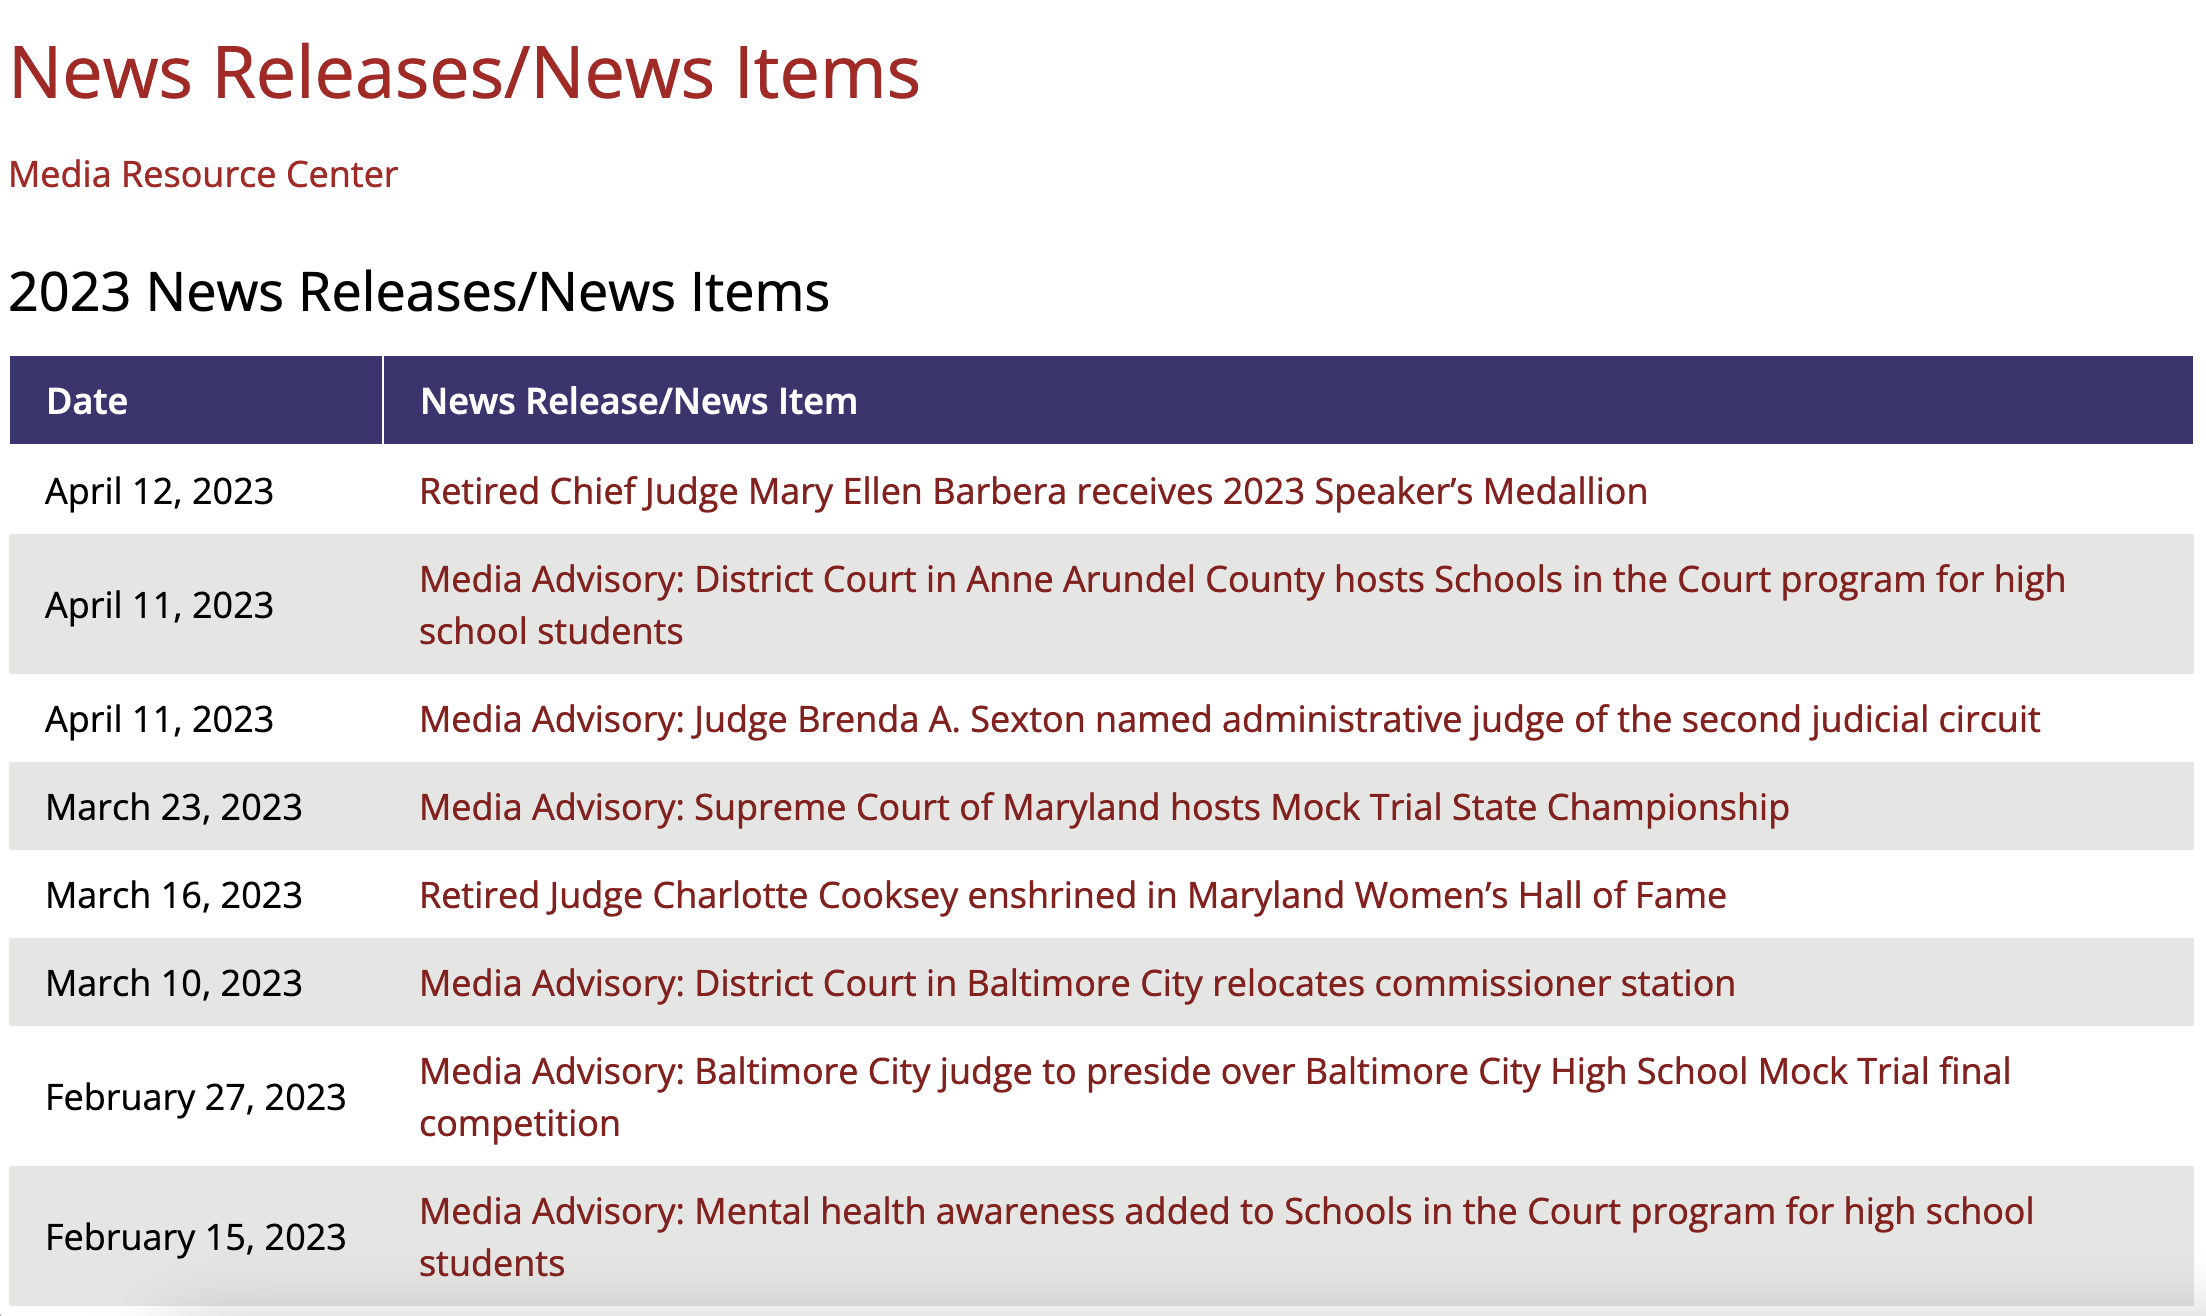
\includegraphics{./images/rvest1.png}

We could get this table into R with the following manual steps:
highlighting the text, copying it into Excel, saving it as a csv, and
reading it into R. Or, we could write a few lines of webscraping code to
have R do that for us!

In this simple example, it's probably faster to do it manually than have
R do it for us. And this table is unlikely to change much in the future.

Why would we ever write code to grab a single table? There's several
reasons:

\begin{enumerate}
\def\labelenumi{\arabic{enumi}.}
\tightlist
\item
  Our methods are transparent. If a colleague wants to run our code from
  scratch to factcheck our work, they don't need to repeat the manual
  steps, which are harder to document than writing code.
\item
  Let's suppose we wanted to grab the same table every day, to monitor
  for changes (like, say, a table on a health department website that
  has COVID case numbers that update every day). Writing a script once,
  and pressing a single button every day is going to be much more
  efficient than doing this manually every day.
\item
  If we're doing it manually, we're more likely to make a mistake, like
  maybe failing to copy every row from the whole table.
\item
  It's good practice to prepare us to do more complex scraping jobs. As
  we'll see in the next chapter, if we ever want to grab the same table
  from hundreds of pages, writing code is much faster and easier than
  going to a hundred different pages ourselves and downloading data.
\end{enumerate}

So, to scrape, the first thing we need to do is start with the URL.
Let's store it as an object called naics\_url.

\begin{Shaded}
\begin{Highlighting}[]
\NormalTok{sboe\_url }\OtherTok{\textless{}{-}} \StringTok{"https://elections.maryland.gov/elections/2022/primary\_results/gen\_detail\_results\_2022\_1\_1\_Republican.html"}
\end{Highlighting}
\end{Shaded}

When we go to the web page, we can see a nicely-designed page that
contains our information.

But what we really care about, for our purposes, is the html code that
creates that page.

In our web browser, if we right-click anywhere on the page and select
``view source'' from the popup menu, we can see the source code. Or you
can just copy this into Google Chrome:
view-source:https://elections.maryland.gov/elections/2022/primary\_results/gen\_detail\_results\_2022\_1\_1\_Republican.html.

Here's a picture of what some of the source code looks like.

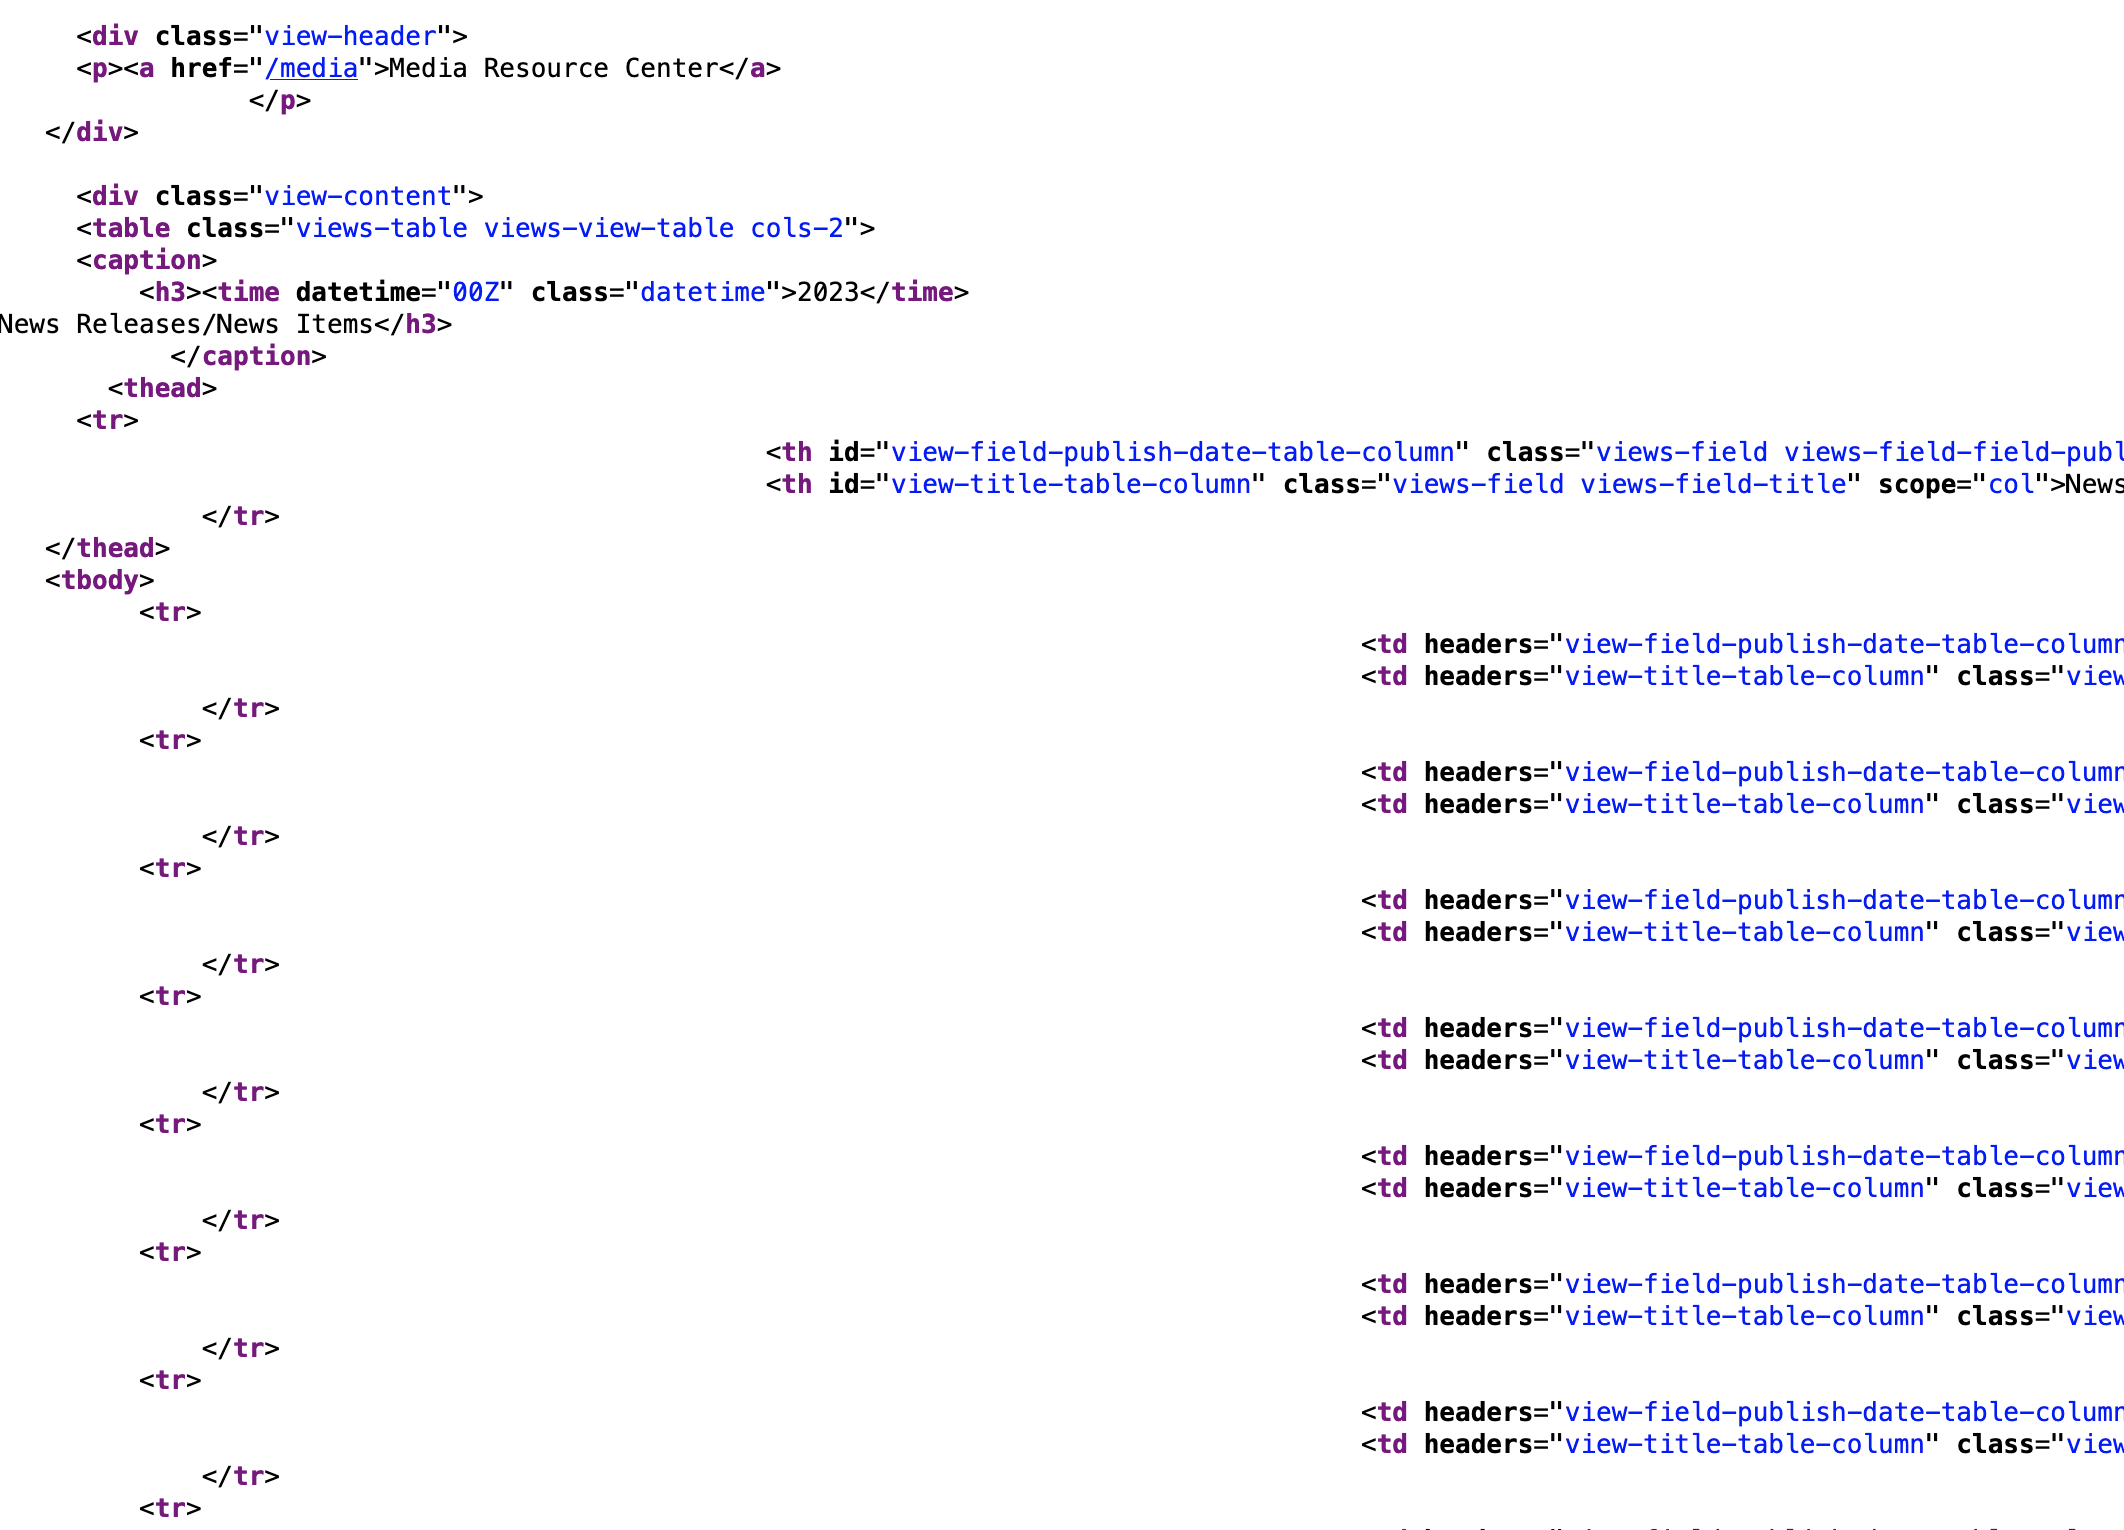
\includegraphics{./images/rvest2.png}

We'll use those HTML tags -- things like
\texttt{\textless{}table\textgreater{}} and
\texttt{\textless{}tr\textgreater{}} -- to grab the info we need.

Okay, step 1.

Let's write a bit of code to tell R to go to the URL for the page and
ingest all of that HTML code. In the code below, we're starting with our
URL and using the read\_html() function from rvest to ingest all of the
page html, storing it as an object called naics\_industry.

\begin{Shaded}
\begin{Highlighting}[]
\CommentTok{\# read in the html}
\NormalTok{results }\OtherTok{\textless{}{-}}\NormalTok{ sboe\_url }\SpecialCharTok{\%\textgreater{}\%}
  \FunctionTok{read\_html}\NormalTok{()}

\CommentTok{\# display the html below}
\NormalTok{results}
\end{Highlighting}
\end{Shaded}

\begin{verbatim}
{html_document}
<html lang="en">
[1] <head>\n<meta http-equiv="Content-Type" content="text/html; charset=UTF-8 ...
[2] <body>\n      <div class="container">\n      <div class="skipNav">\n      ...
\end{verbatim}

If you're running this code in R Studio, in our environment window at
right, you'll see results as a ``list of 2''.

This is not a dataframe, it's a different type of data structure a
``nested list.''

If we click on the name ``results'' in our environment window, we can
see that it's pulled in the html and shown us the general page
structure. Nested within the \texttt{\textless{}html\textgreater{}} tag
is the \texttt{\textless{}head\textgreater{}} and
\texttt{\textless{}body\textgreater{}}, the two fundamental sections of
most web pages. We're going to pull information out of the
\texttt{\textless{}body\textgreater{}} tag in a bit.

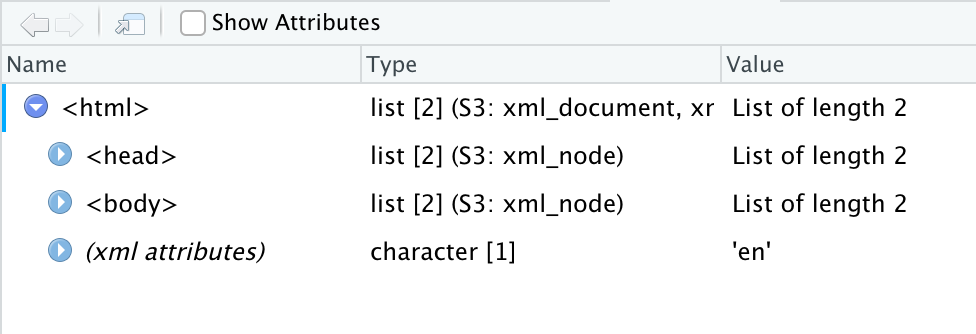
\includegraphics{./images/rvest3.png}

Now, our task is to just pull out the section of the html that contains
the information we need.

But which part do we need from that mess of html code? To figure that
out, we can go back to the page in a web browser like chrome, and use
built in developer tools to ``inspect'' the html code underlying the
page.

On the page, find the data we want to grab -- ``Table 2. NAICS Sectors''
- and right click on the word ``Sector'' in the column header of the
table. That will bring up a dropdown menu. Select ``Inspect'', which
will pop up a window called the ``element inspector'' that shows us
where different elements on the page are located, what html tags created
those elements, and other info.

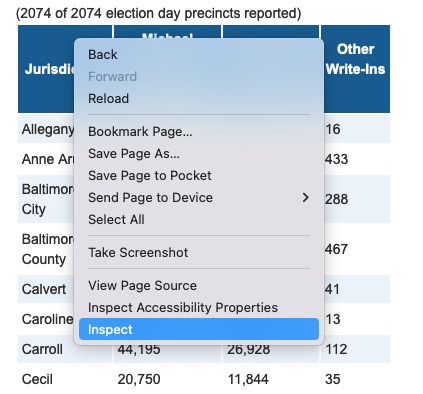
\includegraphics{./images/rvest4.png}

The entire table that we want of results is actually contained inside an
html \texttt{\textless{}table\textgreater{}}. It has a
\texttt{\textless{}tbody\textgreater{}} that contains one row
\texttt{\textless{}tr\textgreater{}} per county.

Because it's inside of a table, and not some other kind of element (like
a \texttt{\textless{}div\textgreater{}}), rvest has a special function
for easily extracting and converting html tables, called html\_table().
This function extracts all the html tables on the page, but this page
only has one so we're good.

\begin{Shaded}
\begin{Highlighting}[]
\CommentTok{\# read in the html and extract all the tables}
\NormalTok{results }\OtherTok{\textless{}{-}}\NormalTok{ sboe\_url }\SpecialCharTok{\%\textgreater{}\%}
  \FunctionTok{read\_html}\NormalTok{() }\SpecialCharTok{\%\textgreater{}\%}
  \FunctionTok{html\_table}\NormalTok{()}

\CommentTok{\# show the dataframe}

\NormalTok{results}
\end{Highlighting}
\end{Shaded}

\begin{verbatim}
[[1]]
# A tibble: 25 x 5
   Jurisdiction     Dan Cox and Gordana Schifanelli\r\~1 Robin~2 Kelly~3 Joe W~4
   <chr>            <chr>                                <chr>   <chr>   <chr>  
 1 Allegany         4,469                                399     2,259   99     
 2 Anne Arundel     18,039                               711     18,581  513    
 3 Baltimore City   1,771                                168     2,010   156    
 4 Baltimore County 18,129                               842     18,247  649    
 5 Calvert          6,081                                335     3,628   186    
 6 Caroline         2,533                                49      1,409   39     
 7 Carroll          10,462                               404     9,997   268    
 8 Cecil            4,998                                203     3,487   128    
 9 Charles          3,473                                176     1,709   127    
10 Dorchester       2,475                                75      916     42     
# ... with 15 more rows, and abbreviated variable names
#   1: `Dan Cox and Gordana Schifanelli\r\n\r\n\r\nRepublican`,
#   2: `Robin Ficker and LeRoy F. Yegge, Jr.\r\n\r\n\r\nRepublican`,
#   3: `Kelly Schulz and Jeff Woolford\r\n\r\n\r\nRepublican`,
#   4: `Joe Werner and Minh Thanh Luong\r\n\r\n\r\nRepublican`
\end{verbatim}

In the environment window at right, look at results Note that it's now a
``list of 1''.

This gets a little complicated, but what you're seeing here is a nested
list that contains one data frame -- also called tibbles -- one for each
table that exists on the web page we scraped.

So, all we need to do now is to store that single dataframe as an
object. We can do that with this code, which says ``keep only the second
dataframe from our nested list.

\begin{Shaded}
\begin{Highlighting}[]
\CommentTok{\# Read in all html from table, store all tables on page as nested list of dataframes.}
\NormalTok{results }\OtherTok{\textless{}{-}}\NormalTok{ sboe\_url }\SpecialCharTok{\%\textgreater{}\%}
  \FunctionTok{read\_html}\NormalTok{() }\SpecialCharTok{\%\textgreater{}\%}
  \FunctionTok{html\_table}\NormalTok{()}

\CommentTok{\# Just keep the first dataframe in our list}

\NormalTok{results }\OtherTok{\textless{}{-}}\NormalTok{ results[[}\DecValTok{1}\NormalTok{]]}

\CommentTok{\# show the dataframe}

\NormalTok{results}
\end{Highlighting}
\end{Shaded}

\begin{verbatim}
# A tibble: 25 x 5
   Jurisdiction     Dan Cox and Gordana Schifanelli\r\~1 Robin~2 Kelly~3 Joe W~4
   <chr>            <chr>                                <chr>   <chr>   <chr>  
 1 Allegany         4,469                                399     2,259   99     
 2 Anne Arundel     18,039                               711     18,581  513    
 3 Baltimore City   1,771                                168     2,010   156    
 4 Baltimore County 18,129                               842     18,247  649    
 5 Calvert          6,081                                335     3,628   186    
 6 Caroline         2,533                                49      1,409   39     
 7 Carroll          10,462                               404     9,997   268    
 8 Cecil            4,998                                203     3,487   128    
 9 Charles          3,473                                176     1,709   127    
10 Dorchester       2,475                                75      916     42     
# ... with 15 more rows, and abbreviated variable names
#   1: `Dan Cox and Gordana Schifanelli\r\n\r\n\r\nRepublican`,
#   2: `Robin Ficker and LeRoy F. Yegge, Jr.\r\n\r\n\r\nRepublican`,
#   3: `Kelly Schulz and Jeff Woolford\r\n\r\n\r\nRepublican`,
#   4: `Joe Werner and Minh Thanh Luong\r\n\r\n\r\nRepublican`
\end{verbatim}

We now have a proper dataframe, albeit with some lengthy column headers.

From here, we can do a little cleaning. First we'll use clean\_names()
to lower the column names. Then use rename() to replace the candidate
column names with simpler versions. We can just use the column positions
instead of writing out the full names, which is nice.

Then let's use slice() to remove the last row -- row number 25 -- which
contains totals and percentages that we don't need. Finally, we'll make
sure the vote tallies are numbers using mutate and \texttt{gsub()},
which we use to replace all the commas with nothing.

\begin{Shaded}
\begin{Highlighting}[]
\CommentTok{\# Read in all html from table, get the HTML table.}
\NormalTok{results }\OtherTok{\textless{}{-}}\NormalTok{ sboe\_url }\SpecialCharTok{\%\textgreater{}\%}
  \FunctionTok{read\_html}\NormalTok{() }\SpecialCharTok{\%\textgreater{}\%}
  \FunctionTok{html\_table}\NormalTok{()}

\CommentTok{\# Standardize column headers, remove last row}

\NormalTok{results }\OtherTok{\textless{}{-}}\NormalTok{ results[[}\DecValTok{1}\NormalTok{]] }\SpecialCharTok{\%\textgreater{}\%}
  \FunctionTok{clean\_names}\NormalTok{() }\SpecialCharTok{\%\textgreater{}\%}
  \FunctionTok{rename}\NormalTok{(}\AttributeTok{cox =} \DecValTok{2}\NormalTok{, }\AttributeTok{ficker =} \DecValTok{3}\NormalTok{, }\AttributeTok{schulz =} \DecValTok{4}\NormalTok{, }\AttributeTok{werner =} \DecValTok{5}\NormalTok{) }\SpecialCharTok{\%\textgreater{}\%}
  \FunctionTok{slice}\NormalTok{(}\SpecialCharTok{{-}}\DecValTok{25}\NormalTok{) }\SpecialCharTok{\%\textgreater{}\%}
  \FunctionTok{mutate}\NormalTok{(}\AttributeTok{cox =} \FunctionTok{as.numeric}\NormalTok{(}\FunctionTok{gsub}\NormalTok{(}\StringTok{","}\NormalTok{,}\StringTok{""}\NormalTok{, cox))) }\SpecialCharTok{\%\textgreater{}\%}
  \FunctionTok{mutate}\NormalTok{(}\AttributeTok{ficker =} \FunctionTok{as.numeric}\NormalTok{(}\FunctionTok{gsub}\NormalTok{(}\StringTok{","}\NormalTok{,}\StringTok{""}\NormalTok{, ficker))) }\SpecialCharTok{\%\textgreater{}\%}
  \FunctionTok{mutate}\NormalTok{(}\AttributeTok{schulz =} \FunctionTok{as.numeric}\NormalTok{(}\FunctionTok{gsub}\NormalTok{(}\StringTok{","}\NormalTok{,}\StringTok{""}\NormalTok{, schulz))) }\SpecialCharTok{\%\textgreater{}\%}
  \FunctionTok{mutate}\NormalTok{(}\AttributeTok{werner =} \FunctionTok{as.numeric}\NormalTok{(}\FunctionTok{gsub}\NormalTok{(}\StringTok{","}\NormalTok{,}\StringTok{""}\NormalTok{, werner)))}


\CommentTok{\# show the dataframe}
\NormalTok{results}
\end{Highlighting}
\end{Shaded}

\begin{verbatim}
# A tibble: 24 x 5
   jurisdiction       cox ficker schulz werner
   <chr>            <dbl>  <dbl>  <dbl>  <dbl>
 1 Allegany          4469    399   2259     99
 2 Anne Arundel     18039    711  18581    513
 3 Baltimore City    1771    168   2010    156
 4 Baltimore County 18129    842  18247    649
 5 Calvert           6081    335   3628    186
 6 Caroline          2533     49   1409     39
 7 Carroll          10462    404   9997    268
 8 Cecil             4998    203   3487    128
 9 Charles           3473    176   1709    127
10 Dorchester        2475     75    916     42
# ... with 14 more rows
\end{verbatim}

And there we go. We now have a nice tidy dataframe of Maryland GOP
gubernatorial primary results that we could ask some questions of.

\bookmarksetup{startatroot}

\hypertarget{intro-to-apis-the-census}{%
\chapter{Intro to APIs: The Census}\label{intro-to-apis-the-census}}

There is truly an astonishing amount of data collected by the US Census
Bureau. First, there's the Census that most people know -- the every 10
year census. That's the one mandated by the Constitution where the
government attempts to count every person in the US. It's a
mind-boggling feat to even try, and billions get spent on it. That data
is used first for determining how many representatives each state gets
in Congress. From there, the Census gets used to divide up billions of
dollars of federal spending.

To answer the questions the government needs to do that, a ton of data
gets collected. That, unfortunately, means the Census is exceedingly
complicated to work with. The good news is, the Census has an API -- an
application programming interface. What that means is we can get data
directly through the Census Bureau via calls over the internet.

Let's demonstrate.

We're going to use a library called \texttt{tidycensus} which makes
calls to the Census API in a very tidy way, and gives you back tidy
data. That means we don't have to go through the process of importing
the data from a file. I can't tell you how amazing this is, speaking
from experience. The documentation for this library is
\href{https://walker-data.com/tidycensus/}{here}. Another R library for
working with Census APIs (there is more than one) is
\href{https://github.com/hrecht/censusapi}{this one} from Hannah Recht,
a journalist with Kaiser Health News.

First we need to install \texttt{tidycensus} using the console:
\texttt{install.packages("tidycensus",\ dependencies\ =\ TRUE)}. You
also should install the \texttt{sf} and \texttt{rgdal} packages.

\begin{Shaded}
\begin{Highlighting}[]
\FunctionTok{library}\NormalTok{(tidyverse)}
\FunctionTok{library}\NormalTok{(tidycensus)}
\end{Highlighting}
\end{Shaded}

To use the API, you need an API key. To get that, you need to
\href{https://api.census.gov/data/key_signup.html}{apply for an API key
with the Census Bureau}. It takes a few minutes and you need to activate
your key via email. Once you have your key, you need to set that for
this session. Just FYI: Your key is your key. Do not share it around.

\begin{Shaded}
\begin{Highlighting}[]
\FunctionTok{census\_api\_key}\NormalTok{(}\StringTok{"YOUR KEY HERE"}\NormalTok{, }\AttributeTok{install=}\ConstantTok{TRUE}\NormalTok{)}
\end{Highlighting}
\end{Shaded}

The two main functions in tidycensus are \texttt{get\_decennial}, which
retrieves data from the 2000 and 2010 Censuses (and soon the 2020
Census), and \texttt{get\_acs}, which pulls data from the American
Community Survey, a between-Censuses annual survey that provides
estimates, not hard counts, but asks more detailed questions. If you're
new to Census data, there's
\href{http://walker-data.com/umich-workshop/census-data-in-r/slides/\#1}{a
very good set of slides from Kyle Walker}, the creator of tidycensus,
and he's working on a
\href{https://walker-data.com/census-r/index.html}{book} that you can
read for free online.

It's important to keep in mind that Census data represents people - you,
your neighbors and total strangers. It also requires some level of
definitions, especially about race \& ethnicity, that may or may not
match how you define yourself or how others define themselves.

So to give you some idea of how complicated the data is, let's pull up
just one file from the decennial Census. We'll use Summary File 1, or
SF1. That has the major population and housing stuff.

\begin{Shaded}
\begin{Highlighting}[]
\NormalTok{sf1 }\OtherTok{\textless{}{-}} \FunctionTok{load\_variables}\NormalTok{(}\DecValTok{2010}\NormalTok{, }\StringTok{"sf1"}\NormalTok{, }\AttributeTok{cache =} \ConstantTok{TRUE}\NormalTok{)}

\NormalTok{sf1}
\end{Highlighting}
\end{Shaded}

\begin{verbatim}
# A tibble: 8,959 x 3
   name    label                                concept         
   <chr>   <chr>                                <chr>           
 1 H001001 Total                                HOUSING UNITS   
 2 H002001 Total                                URBAN AND RURAL 
 3 H002002 Total!!Urban                         URBAN AND RURAL 
 4 H002003 Total!!Urban!!Inside urbanized areas URBAN AND RURAL 
 5 H002004 Total!!Urban!!Inside urban clusters  URBAN AND RURAL 
 6 H002005 Total!!Rural                         URBAN AND RURAL 
 7 H002006 Total!!Not defined for this file     URBAN AND RURAL 
 8 H003001 Total                                OCCUPANCY STATUS
 9 H003002 Total!!Occupied                      OCCUPANCY STATUS
10 H003003 Total!!Vacant                        OCCUPANCY STATUS
# ... with 8,949 more rows
\end{verbatim}

Note: There are thousands of variables in SF1. That's not a typo. Open
it in your environment by double clicking. As you scroll down, you'll
get an idea of what you've got to choose from.

If you think that's crazy, try the SF3 file from 2000.

\begin{Shaded}
\begin{Highlighting}[]
\NormalTok{sf3 }\OtherTok{\textless{}{-}} \FunctionTok{load\_variables}\NormalTok{(}\DecValTok{2000}\NormalTok{, }\StringTok{"sf3"}\NormalTok{, }\AttributeTok{cache =} \ConstantTok{TRUE}\NormalTok{)}

\NormalTok{sf3}
\end{Highlighting}
\end{Shaded}

\begin{verbatim}
# A tibble: 16,520 x 3
   name    label                                       concept                  
   <chr>   <chr>                                       <chr>                    
 1 H001001 Total                                       HOUSING UNITS [1]        
 2 H002001 Total                                       UNWEIGHTED SAMPLE HOUSIN~
 3 H002002 Total!!Occupied                             UNWEIGHTED SAMPLE HOUSIN~
 4 H002003 Total!!Vacant                               UNWEIGHTED SAMPLE HOUSIN~
 5 H003001 Total                                       100-PERCENT COUNT OF HOU~
 6 H004001 Percent of occupied housing units in sample PERCENT OF HOUSING UNITS~
 7 H004002 Percent of vacant housing units in sample   PERCENT OF HOUSING UNITS~
 8 H005001 Total                                       URBAN AND RURAL [7]      
 9 H005002 Total!!Urban                                URBAN AND RURAL [7]      
10 H005003 Total!!Urban!!Inside urbanized areas        URBAN AND RURAL [7]      
# ... with 16,510 more rows
\end{verbatim}

Yes. That's more than 16,000 variables to choose from. I told you.
Astonishing.

So let's try to answer a question using the Census. What is the fastest
growing state since 2000?

To answer this, we need to pull the total population by state in each of
the decennial census. Here's 2000.

\begin{Shaded}
\begin{Highlighting}[]
\NormalTok{p00 }\OtherTok{\textless{}{-}} \FunctionTok{get\_decennial}\NormalTok{(}\AttributeTok{geography =} \StringTok{"state"}\NormalTok{, }\AttributeTok{variables =} \StringTok{"P001001"}\NormalTok{, }\AttributeTok{year =} \DecValTok{2000}\NormalTok{)}
\end{Highlighting}
\end{Shaded}

Now 2010.

\begin{Shaded}
\begin{Highlighting}[]
\NormalTok{p10 }\OtherTok{\textless{}{-}} \FunctionTok{get\_decennial}\NormalTok{(}\AttributeTok{geography =} \StringTok{"state"}\NormalTok{, }\AttributeTok{variables =} \StringTok{"P001001"}\NormalTok{, }\AttributeTok{year =} \DecValTok{2010}\NormalTok{)}
\end{Highlighting}
\end{Shaded}

Let's take a peek at 2010.

\begin{Shaded}
\begin{Highlighting}[]
\NormalTok{p10}
\end{Highlighting}
\end{Shaded}

As you can see, we have a GEOID, NAME, then variable and value. Variable
and value are going to be the same. Because those are named the same
thing, to merge them together, we need to rename them.

\begin{Shaded}
\begin{Highlighting}[]
\NormalTok{p10 }\SpecialCharTok{\%\textgreater{}\%} \FunctionTok{select}\NormalTok{(GEOID, NAME, value) }\SpecialCharTok{\%\textgreater{}\%} \FunctionTok{rename}\NormalTok{(}\AttributeTok{Population2010=}\NormalTok{value) }\OtherTok{{-}\textgreater{}}\NormalTok{ p2010}

\NormalTok{p00 }\SpecialCharTok{\%\textgreater{}\%} \FunctionTok{select}\NormalTok{(GEOID, NAME, value) }\SpecialCharTok{\%\textgreater{}\%} \FunctionTok{rename}\NormalTok{(}\AttributeTok{Population2000=}\NormalTok{value) }\OtherTok{{-}\textgreater{}}\NormalTok{ p2000}
\end{Highlighting}
\end{Shaded}

Now we join the data together.

\begin{Shaded}
\begin{Highlighting}[]
\NormalTok{alldata }\OtherTok{\textless{}{-}}\NormalTok{ p2000 }\SpecialCharTok{\%\textgreater{}\%} \FunctionTok{inner\_join}\NormalTok{(p2010)}
\end{Highlighting}
\end{Shaded}

And now we calculate the percent change.

\begin{Shaded}
\begin{Highlighting}[]
\NormalTok{alldata }\SpecialCharTok{\%\textgreater{}\%} \FunctionTok{mutate}\NormalTok{(}\AttributeTok{change =}\NormalTok{ ((Population2010}\SpecialCharTok{{-}}\NormalTok{Population2000)}\SpecialCharTok{/}\NormalTok{Population2000)}\SpecialCharTok{*}\DecValTok{100}\NormalTok{) }\SpecialCharTok{\%\textgreater{}\%} \FunctionTok{arrange}\NormalTok{(}\FunctionTok{desc}\NormalTok{(change))}
\end{Highlighting}
\end{Shaded}

And just like that: Nevada.

You may be asking: hey, wasn't there a 2020 Census? Where's that data?
The answer is that it's coming, slowly - the Census Bureau has a
\href{https://www.census.gov/programs-surveys/popest/about/schedule.html}{schedule
of releases}.

\hypertarget{the-acs}{%
\section{The ACS}\label{the-acs}}

In 2010, the Census Bureau replaced SF3 with the American Community
Survey. The Good News is that the data would be updated on a rolling
basis. The bad news is that it's more complicated because it's more like
survey data with a large sample. That means there's margins of error and
confidence intervals to worry about. By default, using \texttt{get\_acs}
fetches data from the 5-year estimates (currently 2016-2020), but you
can specify 1-year estimates for jurisdictions with at least 65,000
people (many counties and cities).

Here's an example using the 5-year ACS estimates:

What is Maryland's richest county?

We can measure this by median household income. That variable is
\texttt{B19013\_001}, so we can get that data like this (I'm narrowing
it to the top 20 for simplicity):

\begin{Shaded}
\begin{Highlighting}[]
\NormalTok{md }\OtherTok{\textless{}{-}} \FunctionTok{get\_acs}\NormalTok{(}\AttributeTok{geography =} \StringTok{"county"}\NormalTok{,}
              \AttributeTok{variables =} \FunctionTok{c}\NormalTok{(}\AttributeTok{medincome =} \StringTok{"B19013\_001"}\NormalTok{),}
              \AttributeTok{state =} \StringTok{"MD"}\NormalTok{,}
              \AttributeTok{year =} \DecValTok{2020}\NormalTok{)}
\end{Highlighting}
\end{Shaded}

\begin{verbatim}
Getting data from the 2016-2020 5-year ACS
\end{verbatim}

\begin{Shaded}
\begin{Highlighting}[]
\NormalTok{md }\OtherTok{\textless{}{-}}\NormalTok{ md }\SpecialCharTok{\%\textgreater{}\%} \FunctionTok{arrange}\NormalTok{(}\FunctionTok{desc}\NormalTok{(estimate)) }\SpecialCharTok{\%\textgreater{}\%} \FunctionTok{top\_n}\NormalTok{(}\DecValTok{20}\NormalTok{, estimate)}

\NormalTok{md}
\end{Highlighting}
\end{Shaded}

\begin{verbatim}
# A tibble: 20 x 5
   GEOID NAME                             variable  estimate   moe
   <chr> <chr>                            <chr>        <dbl> <dbl>
 1 24027 Howard County, Maryland          medincome   124042  3448
 2 24009 Calvert County, Maryland         medincome   112696  3287
 3 24031 Montgomery County, Maryland      medincome   111812  1361
 4 24017 Charles County, Maryland         medincome   103678  1654
 5 24003 Anne Arundel County, Maryland    medincome   103225  1817
 6 24021 Frederick County, Maryland       medincome   100685  1927
 7 24013 Carroll County, Maryland         medincome    99569  3051
 8 24035 Queen Anne's County, Maryland    medincome    96467  4785
 9 24037 St. Mary's County, Maryland      medincome    95864  3872
10 24025 Harford County, Maryland         medincome    94003  2398
11 24033 Prince George's County, Maryland medincome    86994   865
12 24015 Cecil County, Maryland           medincome    79415  3479
13 24005 Baltimore County, Maryland       medincome    78724  1641
14 24041 Talbot County, Maryland          medincome    73102  4031
15 24047 Worcester County, Maryland       medincome    65396  3856
16 24043 Washington County, Maryland      medincome    63510  1930
17 24045 Wicomico County, Maryland        medincome    60366  2437
18 24029 Kent County, Maryland            medincome    60208  5185
19 24011 Caroline County, Maryland        medincome    59042  4215
20 24023 Garrett County, Maryland         medincome    54542  3487
\end{verbatim}

Howard, Calvert, Montgomery, Anne Arundel, Charles. What do they all
have in common? Lots of suburban flight from DC and Baltimore. But do
the margins of error let us say one county is richer than the other. We
can find this out visually using error bars. Don't worry much about the
code here -- we'll cover that soon enough.

\begin{Shaded}
\begin{Highlighting}[]
\NormalTok{md }\SpecialCharTok{\%\textgreater{}\%}
  \FunctionTok{mutate}\NormalTok{(}\AttributeTok{NAME =} \FunctionTok{gsub}\NormalTok{(}\StringTok{" County, Maryland"}\NormalTok{, }\StringTok{""}\NormalTok{, NAME)) }\SpecialCharTok{\%\textgreater{}\%}
  \FunctionTok{ggplot}\NormalTok{(}\FunctionTok{aes}\NormalTok{(}\AttributeTok{x =}\NormalTok{ estimate, }\AttributeTok{y =} \FunctionTok{reorder}\NormalTok{(NAME, estimate))) }\SpecialCharTok{+}
  \FunctionTok{geom\_errorbarh}\NormalTok{(}\FunctionTok{aes}\NormalTok{(}\AttributeTok{xmin =}\NormalTok{ estimate }\SpecialCharTok{{-}}\NormalTok{ moe, }\AttributeTok{xmax =}\NormalTok{ estimate }\SpecialCharTok{+}\NormalTok{ moe)) }\SpecialCharTok{+}
  \FunctionTok{geom\_point}\NormalTok{(}\AttributeTok{color =} \StringTok{"red"}\NormalTok{) }\SpecialCharTok{+}
  \FunctionTok{labs}\NormalTok{(}\AttributeTok{title =} \StringTok{"Household income by county in Maryland"}\NormalTok{,}
       \AttributeTok{subtitle =} \StringTok{"2016{-}2020 American Community Survey"}\NormalTok{,}
       \AttributeTok{y =} \StringTok{""}\NormalTok{,}
       \AttributeTok{x =} \StringTok{"ACS estimate (bars represent margin of error)"}\NormalTok{)}
\end{Highlighting}
\end{Shaded}

\begin{figure}[H]

{\centering 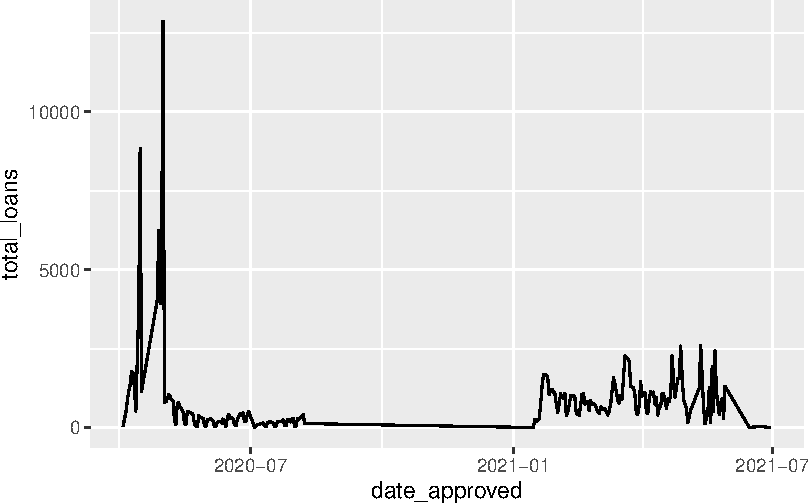
\includegraphics{./census_files/figure-pdf/unnamed-chunk-13-1.pdf}

}

\end{figure}

As you can see, some of the error bars are quite wide. Some are narrow.
But if the bars overlap, it means the difference between the two
counties is within the margin of error, and the differences aren't
statistically significant. So is the difference between Calvert and
Montgomery significant? Nope. Is the difference between Howard and
everyone else significant? Yes it is.

Let's ask another question of the ACS -- did any counties lose income
from the time of the global financial crisis to the current 5-year
window?

Let's re-label our first household income data.

\begin{Shaded}
\begin{Highlighting}[]
\NormalTok{md20 }\OtherTok{\textless{}{-}} \FunctionTok{get\_acs}\NormalTok{(}\AttributeTok{geography =} \StringTok{"county"}\NormalTok{,}
              \AttributeTok{variables =} \FunctionTok{c}\NormalTok{(}\AttributeTok{medincome =} \StringTok{"B19013\_001"}\NormalTok{),}
              \AttributeTok{state =} \StringTok{"MD"}\NormalTok{,}
              \AttributeTok{year =} \DecValTok{2020}\NormalTok{)}
\end{Highlighting}
\end{Shaded}

\begin{verbatim}
Getting data from the 2016-2020 5-year ACS
\end{verbatim}

And now we grab the 2010 median household income.

\begin{Shaded}
\begin{Highlighting}[]
\NormalTok{md10 }\OtherTok{\textless{}{-}} \FunctionTok{get\_acs}\NormalTok{(}\AttributeTok{geography =} \StringTok{"county"}\NormalTok{,}
              \AttributeTok{variables =} \FunctionTok{c}\NormalTok{(}\AttributeTok{medincome =} \StringTok{"B19013\_001"}\NormalTok{),}
              \AttributeTok{state =} \StringTok{"MD"}\NormalTok{,}
              \AttributeTok{year =} \DecValTok{2010}\NormalTok{)}
\end{Highlighting}
\end{Shaded}

\begin{verbatim}
Getting data from the 2006-2010 5-year ACS
\end{verbatim}

What I'm going to do next is a lot, but each step is simple. I'm going
to join the data together, so each county has one line of data. Then I'm
going to rename some fields that repeat. Then I'm going to calculate the
minimium and maximum value of the estimate using the margin of error.
That'll help me later. After that, I'm going to calculate a perent
change and sort it by that change.

\begin{Shaded}
\begin{Highlighting}[]
\NormalTok{md10 }\SpecialCharTok{\%\textgreater{}\%}
  \FunctionTok{inner\_join}\NormalTok{(md20, }\AttributeTok{by=}\FunctionTok{c}\NormalTok{(}\StringTok{"GEOID"}\NormalTok{, }\StringTok{"NAME"}\NormalTok{)) }\SpecialCharTok{\%\textgreater{}\%}
  \FunctionTok{rename}\NormalTok{(}\AttributeTok{estimate2010=}\NormalTok{estimate.x, }\AttributeTok{estimate2020=}\NormalTok{estimate.y) }\SpecialCharTok{\%\textgreater{}\%}
  \FunctionTok{mutate}\NormalTok{(}\AttributeTok{min2010 =}\NormalTok{ estimate2010}\SpecialCharTok{{-}}\NormalTok{moe.x, }\AttributeTok{max2010 =}\NormalTok{ estimate2010}\SpecialCharTok{+}\NormalTok{moe.x, }\AttributeTok{min2020 =}\NormalTok{ estimate2020}\SpecialCharTok{{-}}\NormalTok{moe.y, }\AttributeTok{max2020 =}\NormalTok{ estimate2020}\SpecialCharTok{+}\NormalTok{moe.y) }\SpecialCharTok{\%\textgreater{}\%}
  \FunctionTok{select}\NormalTok{(}\SpecialCharTok{{-}}\NormalTok{variable.x, }\SpecialCharTok{{-}}\NormalTok{variable.y, }\SpecialCharTok{{-}}\NormalTok{moe.x, }\SpecialCharTok{{-}}\NormalTok{moe.y) }\SpecialCharTok{\%\textgreater{}\%}
  \FunctionTok{mutate}\NormalTok{(}\AttributeTok{change =}\NormalTok{ ((estimate2020}\SpecialCharTok{{-}}\NormalTok{estimate2010)}\SpecialCharTok{/}\NormalTok{estimate2010)}\SpecialCharTok{*}\DecValTok{100}\NormalTok{) }\SpecialCharTok{\%\textgreater{}\%}
  \FunctionTok{arrange}\NormalTok{(change)}
\end{Highlighting}
\end{Shaded}

\begin{verbatim}
# A tibble: 24 x 9
   GEOID NAME             estim~1 estim~2 min2010 max2010 min2020 max2020 change
   <chr> <chr>              <dbl>   <dbl>   <dbl>   <dbl>   <dbl>   <dbl>  <dbl>
 1 24011 Caroline County~   58799   59042   56740   60858   54827   63257  0.413
 2 24039 Somerset County~   42443   44980   39092   45794   40432   49528  5.98 
 3 24041 Talbot County, ~   63017   73102   60081   65953   69071   77133 16.0  
 4 24017 Charles County,~   88825  103678   87268   90382  102024  105332 16.7  
 5 24019 Dorchester Coun~   45151   52799   43470   46832   49020   56578 16.9  
 6 24047 Worcester Count~   55487   65396   52749   58225   61540   69252 17.9  
 7 24045 Wicomico County~   50752   60366   49313   52191   57929   62803 18.9  
 8 24035 Queen Anne's Co~   81096   96467   78068   84124   91682  101252 19.0  
 9 24023 Garrett County,~   45760   54542   43729   47791   51055   58029 19.2  
10 24031 Montgomery Coun~   93373  111812   92535   94211  110451  113173 19.7  
# ... with 14 more rows, and abbreviated variable names 1: estimate2010,
#   2: estimate2020
\end{verbatim}

So according to this, Somerset and Caroline counties had the smallest
change between 2010 and 2020, while all other jurisdictions saw
double-digit percentage increases.

But did they?

Look at the min and max values for both. Is the change statistically
significant?

The ACS data has lots of variables, just like the decennial Census does.
To browse them, you can do this:

\begin{Shaded}
\begin{Highlighting}[]
\NormalTok{v20 }\OtherTok{\textless{}{-}} \FunctionTok{load\_variables}\NormalTok{(}\DecValTok{2020}\NormalTok{, }\StringTok{"acs5"}\NormalTok{, }\AttributeTok{cache=}\ConstantTok{TRUE}\NormalTok{)}
\end{Highlighting}
\end{Shaded}

And then view \texttt{v20} to see what kinds of variables are available
via the API.

\hypertarget{wide-results}{%
\section{``Wide'' Results}\label{wide-results}}

Although one of the chief strengths of tidycensus is that it offers a,
well, tidy display of Census data, it also has the ability to view
multiple variables spread across columns. This can be useful for
creating percentages and comparing multiple variables.

\hypertarget{sorting-results}{%
\section{Sorting Results}\label{sorting-results}}

You'll notice that we've used \texttt{arrange} to sort the results of
tidycensus functions, although that's done after we create a new
variable to hold the data. There's another way to use \texttt{arrange}
that you should know about, one that you can use for exploratory
analysis. An example using median household income from 2020:

\begin{Shaded}
\begin{Highlighting}[]
\NormalTok{md20 }\OtherTok{\textless{}{-}} \FunctionTok{get\_acs}\NormalTok{(}\AttributeTok{geography =} \StringTok{"county"}\NormalTok{,}
              \AttributeTok{variables =} \FunctionTok{c}\NormalTok{(}\AttributeTok{medincome =} \StringTok{"B19013\_001"}\NormalTok{),}
              \AttributeTok{state =} \StringTok{"MD"}\NormalTok{,}
              \AttributeTok{year =} \DecValTok{2020}\NormalTok{)}
\end{Highlighting}
\end{Shaded}

\begin{verbatim}
Getting data from the 2016-2020 5-year ACS
\end{verbatim}

\begin{Shaded}
\begin{Highlighting}[]
\FunctionTok{arrange}\NormalTok{(md20, }\FunctionTok{desc}\NormalTok{(estimate))}
\end{Highlighting}
\end{Shaded}

\begin{verbatim}
# A tibble: 24 x 5
   GEOID NAME                          variable  estimate   moe
   <chr> <chr>                         <chr>        <dbl> <dbl>
 1 24027 Howard County, Maryland       medincome   124042  3448
 2 24009 Calvert County, Maryland      medincome   112696  3287
 3 24031 Montgomery County, Maryland   medincome   111812  1361
 4 24017 Charles County, Maryland      medincome   103678  1654
 5 24003 Anne Arundel County, Maryland medincome   103225  1817
 6 24021 Frederick County, Maryland    medincome   100685  1927
 7 24013 Carroll County, Maryland      medincome    99569  3051
 8 24035 Queen Anne's County, Maryland medincome    96467  4785
 9 24037 St. Mary's County, Maryland   medincome    95864  3872
10 24025 Harford County, Maryland      medincome    94003  2398
# ... with 14 more rows
\end{verbatim}

In this case we don't save the sorted results to a variable, we can just
see the output in the console.

\bookmarksetup{startatroot}

\hypertarget{visualizing-your-data-for-reporting}{%
\chapter{Visualizing your data for
reporting}\label{visualizing-your-data-for-reporting}}

Visualizing data is becoming a much greater part of journalism. Large
news organizations are creating graphics desks that create complex
visuals with data to inform the public about important events.

To do it well is a course on its own. And not every story needs a feat
of programming and art. Sometimes, you can help yourself and your story
by just creating a quick chart, which helps you see patterns in the data
that wouldn't otherwise surface.

Good news: one of the best libraries for visualizing data is in the
tidyverse and it's pretty simple to make simple charts quickly with just
a little bit of code. It's called
\href{https://ggplot2.tidyverse.org/}{ggplot2}.

Let's revisit some data we've used in the past and turn it into charts.
First, let's load libraries. When we load the tidyverse, we get ggplot2.

\begin{Shaded}
\begin{Highlighting}[]
\FunctionTok{library}\NormalTok{(tidyverse)}
\end{Highlighting}
\end{Shaded}

The dataset we'll use is the voter registration data for Maryland. Let's
load it.

\begin{Shaded}
\begin{Highlighting}[]
\NormalTok{ppp\_maryland }\OtherTok{\textless{}{-}} \FunctionTok{read\_csv}\NormalTok{(}\StringTok{"pre\_labs/pre\_lab\_09/data/ppp\_loans\_md.csv.zip"}\NormalTok{)}
\end{Highlighting}
\end{Shaded}

\begin{verbatim}
Rows: 195865 Columns: 63
-- Column specification --------------------------------------------------------
Delimiter: ","
chr  (32): name, slug, state, address, city, zip, business_type, race, gende...
dbl  (21): id, amount, naics_code, jobs_retained, loan_number, sba_office_co...
lgl   (7): non_profit, loan_range_sort_key, previous_loan_range, previous_na...
date  (3): date_approved, loan_status_date, forgiveness_date

i Use `spec()` to retrieve the full column specification for this data.
i Specify the column types or set `show_col_types = FALSE` to quiet this message.
\end{verbatim}

\hypertarget{bar-charts}{%
\section{Bar charts}\label{bar-charts}}

The first kind of chart we'll create is a simple bar chart.

It's a chart designed to show differences between things -- the
magnitude of one thing, compared to the next thing, and the next, and
the next.

So if we have thing, like a county, or a state, or a group name, and
then a count of that group, we can make a bar chart.

So what does the chart of the top 10 maryland counties with the most
total PPP loans look like?

First, we'll create a dataframe of those top 10, called
maryland\_ppp\_top\_counties.

\begin{Shaded}
\begin{Highlighting}[]
\NormalTok{maryland\_ppp\_top\_counties }\OtherTok{\textless{}{-}}\NormalTok{ ppp\_maryland }\SpecialCharTok{\%\textgreater{}\%}
  \FunctionTok{group\_by}\NormalTok{(project\_county\_name) }\SpecialCharTok{\%\textgreater{}\%}
  \FunctionTok{summarise}\NormalTok{(}
    \AttributeTok{total\_loans =} \FunctionTok{n}\NormalTok{()}
\NormalTok{  ) }\SpecialCharTok{\%\textgreater{}\%}
  \FunctionTok{arrange}\NormalTok{(}\FunctionTok{desc}\NormalTok{(total\_loans)) }\SpecialCharTok{\%\textgreater{}\%}
  \FunctionTok{head}\NormalTok{(}\DecValTok{10}\NormalTok{)}

\NormalTok{maryland\_ppp\_top\_counties}
\end{Highlighting}
\end{Shaded}

\begin{verbatim}
# A tibble: 10 x 2
   project_county_name total_loans
   <chr>                     <int>
 1 MONTGOMERY                38782
 2 PRINCE GEORGES            34409
 3 BALTIMORE                 28789
 4 BALTIMORE CITY            20004
 5 ANNE ARUNDEL              17336
 6 HOWARD                    12011
 7 FREDERICK                  6666
 8 HARFORD                    6301
 9 CHARLES                    4398
10 CARROLL                    4040
\end{verbatim}

Now let's create a bar chart using ggplot.

With ggplot, the first thing we'll always do is draw a blank canvas that
will house our chart. We start with our dataframe name, and then
(\%\textgreater\%) we invoke the ggplot() function to make that blank
canvas. All this does is make a gray box, the blank canvas that will
hold our chart.

\begin{Shaded}
\begin{Highlighting}[]
\NormalTok{maryland\_ppp\_top\_counties }\SpecialCharTok{\%\textgreater{}\%}
  \FunctionTok{ggplot}\NormalTok{()}
\end{Highlighting}
\end{Shaded}

\begin{figure}[H]

{\centering 
\includegraphics{./visualizing-for-reporting_files/figure-pdf/unnamed-chunk-4-1.pdf}

}

\end{figure}

Next we need to tell ggplot what kind of chart to make.

In ggplot, we work with two key concepts called geometries (abbreivated
frequently as geom) and asthetics (abbreviated as aes).

Geometries are the shape that the data will take; think of line charts,
bar charts, scatterplots, histograms, pie charts and other common
graphics forms.

Asesthetics help ggplot know what component of our data to visualize --
why we'll visualize values from one column instead of another.

In a bar chart, we first pass in the data to the geometry, then set the
aesthetic.

In the codeblock below, we've added a new function, geom\_bar().

Using geom\_bar() -- as opposed to geom\_line() -- says we're making a
bar chart.

Inside of that function, the asthetic, aes, says which columns to use in
drawing the chart.

We're setting the values on the x axis (horizontal) to be the name of
the county. We set weight to total loans, and it uses that value to
``weight'' or set the height of each bar.

One quirk here with ggplot.

After we've invoked the ggplot() function, you'll notice we're using a +
symbol. It means the same thing as \%\textgreater\% -- ``and then do
this''. It's just a quirk of ggplot() that after you invoke the ggplot()
function, you use + instead of \%\textgreater\%. It makes no sense to me
either, just something to live with.

\begin{Shaded}
\begin{Highlighting}[]
\NormalTok{maryland\_ppp\_top\_counties }\SpecialCharTok{\%\textgreater{}\%}
  \FunctionTok{ggplot}\NormalTok{() }\SpecialCharTok{+}
  \FunctionTok{geom\_bar}\NormalTok{(}\FunctionTok{aes}\NormalTok{(}\AttributeTok{x=}\NormalTok{project\_county\_name, }\AttributeTok{weight=}\NormalTok{total\_loans))}
\end{Highlighting}
\end{Shaded}

\begin{figure}[H]

{\centering 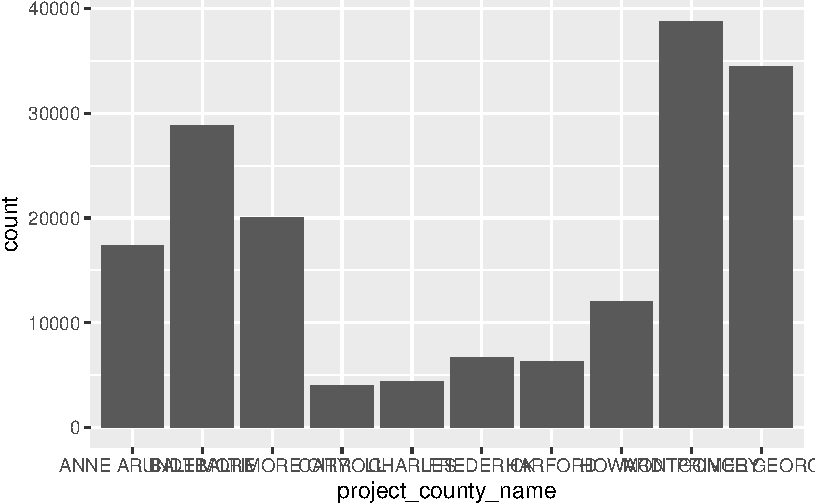
\includegraphics{./visualizing-for-reporting_files/figure-pdf/unnamed-chunk-5-1.pdf}

}

\end{figure}

This is a very basic chart. But it's hard to derive much meaning from
this chart, because the counties aren't ordered from highest to lowest
by total\_loans. We can fix that by using the reorder() function to do
just that:

\begin{Shaded}
\begin{Highlighting}[]
\NormalTok{maryland\_ppp\_top\_counties }\SpecialCharTok{\%\textgreater{}\%}
  \FunctionTok{ggplot}\NormalTok{() }\SpecialCharTok{+}
  \FunctionTok{geom\_bar}\NormalTok{(}\FunctionTok{aes}\NormalTok{(}\AttributeTok{x=}\FunctionTok{reorder}\NormalTok{(project\_county\_name,total\_loans), }\AttributeTok{weight=}\NormalTok{total\_loans))}
\end{Highlighting}
\end{Shaded}

\begin{figure}[H]

{\centering 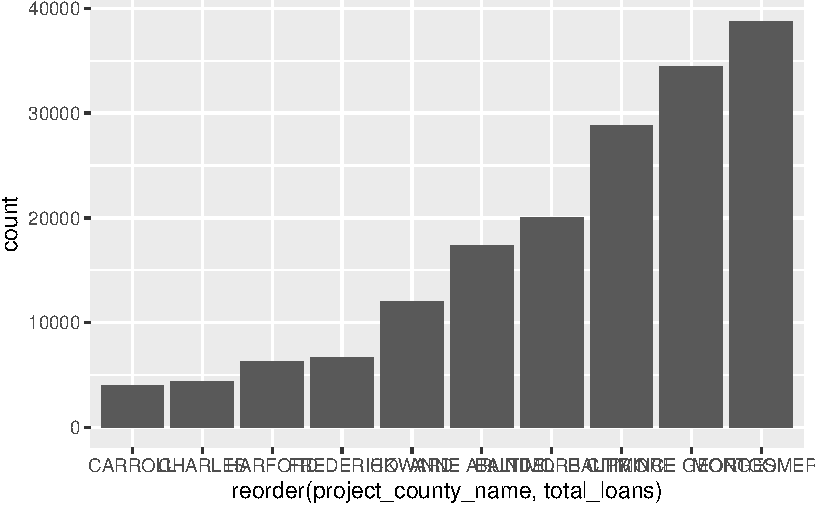
\includegraphics{./visualizing-for-reporting_files/figure-pdf/unnamed-chunk-6-1.pdf}

}

\end{figure}

This is a little more useful. But the bottom is kind of a mess, with
overlapping names. We can fix that by flipping it from a vertical bar
chart (also called a column chart) to a horizontal one. coord\_flip()
does that for you.

\begin{Shaded}
\begin{Highlighting}[]
\NormalTok{maryland\_ppp\_top\_counties }\SpecialCharTok{\%\textgreater{}\%}
  \FunctionTok{ggplot}\NormalTok{() }\SpecialCharTok{+}
  \FunctionTok{geom\_bar}\NormalTok{(}\FunctionTok{aes}\NormalTok{(}\AttributeTok{x=}\FunctionTok{reorder}\NormalTok{(project\_county\_name,total\_loans), }\AttributeTok{weight=}\NormalTok{total\_loans)) }\SpecialCharTok{+}
  \FunctionTok{coord\_flip}\NormalTok{()}
\end{Highlighting}
\end{Shaded}

\begin{figure}[H]

{\centering 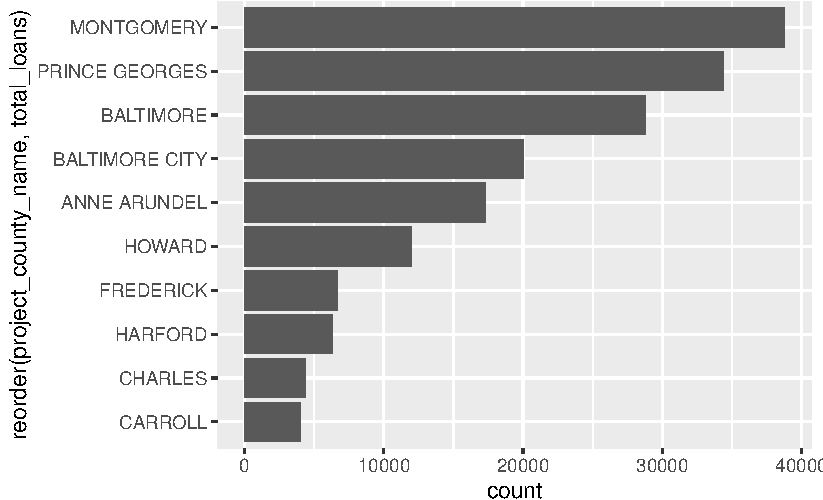
\includegraphics{./visualizing-for-reporting_files/figure-pdf/unnamed-chunk-7-1.pdf}

}

\end{figure}

Is this art? No.~Does it quickly tell you something meaningful? It does.

We're mainly going to use these charts to help us in reporting, so style
isn't that important.

But it's worth mentioning that we can pretty up these charts for
publication, if we wanted to, with some more code. To style the chart,
we can change or even modify the ``theme'', a kind of skin that makes
the chart look better.

It's kind of like applying CSS to html. Here I'm changing the theme
slightly to remove the gray background with one of ggplot's built in
themes, theme\_minimal()

\begin{Shaded}
\begin{Highlighting}[]
\NormalTok{maryland\_ppp\_top\_counties }\SpecialCharTok{\%\textgreater{}\%}
  \FunctionTok{ggplot}\NormalTok{() }\SpecialCharTok{+}
  \FunctionTok{geom\_bar}\NormalTok{(}\FunctionTok{aes}\NormalTok{(}\AttributeTok{x=}\FunctionTok{reorder}\NormalTok{(project\_county\_name,total\_loans), }\AttributeTok{weight=}\NormalTok{total\_loans)) }\SpecialCharTok{+}
  \FunctionTok{coord\_flip}\NormalTok{() }\SpecialCharTok{+}
  \FunctionTok{theme\_minimal}\NormalTok{()}
\end{Highlighting}
\end{Shaded}

\begin{figure}[H]

{\centering 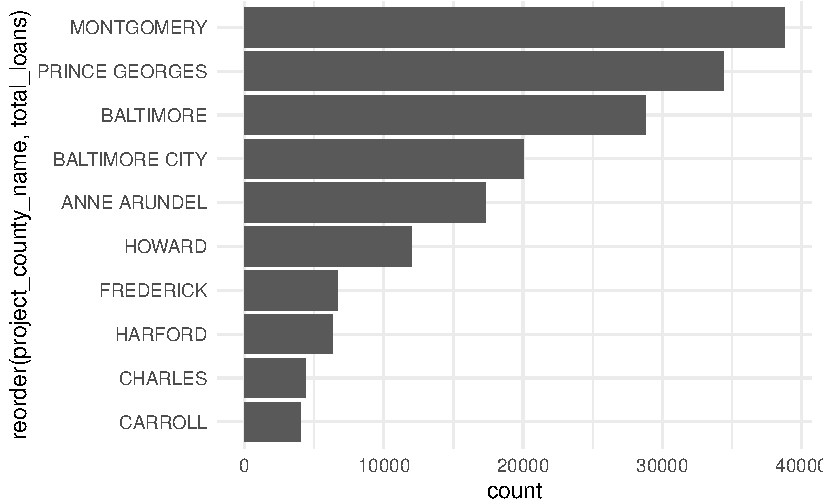
\includegraphics{./visualizing-for-reporting_files/figure-pdf/unnamed-chunk-8-1.pdf}

}

\end{figure}

The ggplot universe is pretty big, and lots of people have made and
released cool themes for you to use. Want to make your graphics look
kind of like \href{https://www.economist.com/}{The Economist's}
graphics? There's a theme for that.

First, you have to install and load a package that contains lots of
extra themes, called
\href{https://yutannihilation.github.io/allYourFigureAreBelongToUs/ggthemes/}{ggthemes}.

\begin{Shaded}
\begin{Highlighting}[]
\CommentTok{\#install.packages(\textquotesingle{}ggthemes\textquotesingle{})}
\FunctionTok{library}\NormalTok{(ggthemes)}
\end{Highlighting}
\end{Shaded}

And now we'll apply the economist theme from that package with
theme\_economist()

\begin{Shaded}
\begin{Highlighting}[]
\NormalTok{maryland\_ppp\_top\_counties }\SpecialCharTok{\%\textgreater{}\%}
  \FunctionTok{ggplot}\NormalTok{() }\SpecialCharTok{+}
  \FunctionTok{geom\_bar}\NormalTok{(}\FunctionTok{aes}\NormalTok{(}\AttributeTok{x=}\FunctionTok{reorder}\NormalTok{(project\_county\_name,total\_loans), }\AttributeTok{weight=}\NormalTok{total\_loans)) }\SpecialCharTok{+}
  \FunctionTok{coord\_flip}\NormalTok{() }\SpecialCharTok{+}
  \FunctionTok{theme\_economist}\NormalTok{()}
\end{Highlighting}
\end{Shaded}

\begin{figure}[H]

{\centering 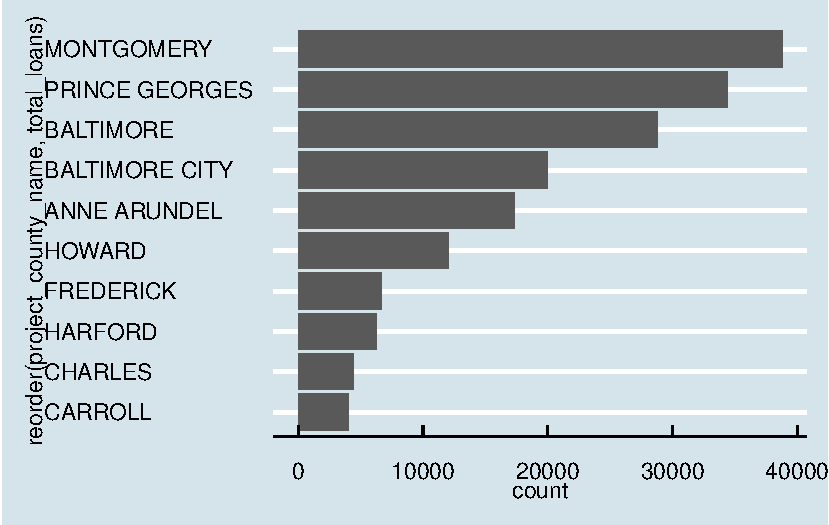
\includegraphics{./visualizing-for-reporting_files/figure-pdf/unnamed-chunk-10-1.pdf}

}

\end{figure}

Those axis titles are kind of a mess. Let's change ``count'' on the x
axis to ``total loans'' and change
``reorder(project\_county\_name,total\_loans)'' to ``county''. And while
we're at it, let's add a basic title and a source as a caption. We'll
use a new function, labs(), which is short for labels.

\begin{Shaded}
\begin{Highlighting}[]
\NormalTok{maryland\_ppp\_top\_counties }\SpecialCharTok{\%\textgreater{}\%}
  \FunctionTok{ggplot}\NormalTok{() }\SpecialCharTok{+}
  \FunctionTok{geom\_bar}\NormalTok{(}\FunctionTok{aes}\NormalTok{(}\AttributeTok{x=}\FunctionTok{reorder}\NormalTok{(project\_county\_name,total\_loans), }\AttributeTok{weight=}\NormalTok{total\_loans)) }\SpecialCharTok{+}
  \FunctionTok{coord\_flip}\NormalTok{() }\SpecialCharTok{+}
  \FunctionTok{theme\_economist}\NormalTok{() }\SpecialCharTok{+}
  \FunctionTok{labs}\NormalTok{(}
    \AttributeTok{title=}\StringTok{"Maryland Counties with Most PPP Loans"}\NormalTok{,}
    \AttributeTok{x =} \StringTok{"total loans"}\NormalTok{,}
    \AttributeTok{y =} \StringTok{"county"}\NormalTok{,}
    \AttributeTok{caption =} \StringTok{"source: SBA PPP loan database"}

\NormalTok{  )}
\end{Highlighting}
\end{Shaded}

\begin{figure}[H]

{\centering 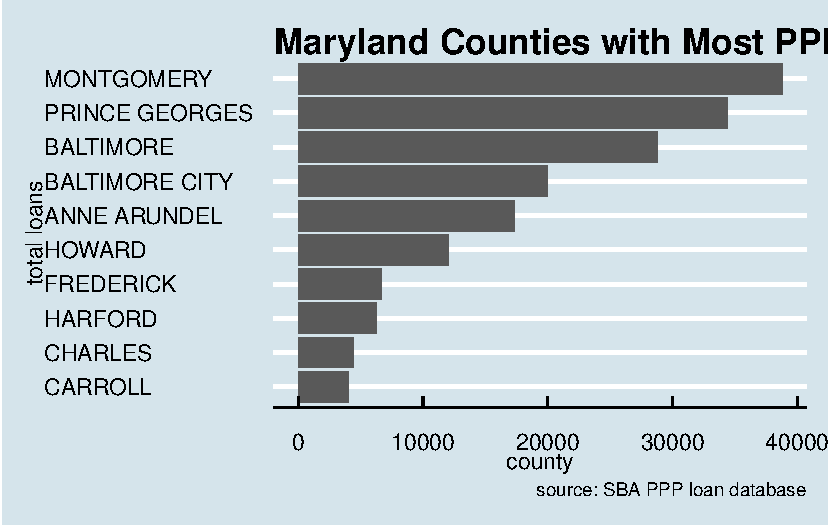
\includegraphics{./visualizing-for-reporting_files/figure-pdf/unnamed-chunk-11-1.pdf}

}

\end{figure}

Viola. Not super pretty, but good enough to show an editor to help them
understand the conclusions you reached with your data analysis.

\hypertarget{line-charts}{%
\section{Line charts}\label{line-charts}}

Let's look at how to make another common chart type that will help you
understand patterns in your data.

Line charts can show change over time. It works much the same as a bar
chart, code wise, but instead of a weight, it uses a y.

So, let's create a dataframe with a count of Maryland loans for each
date in our dataframe.

\begin{Shaded}
\begin{Highlighting}[]
\NormalTok{ppp\_maryland\_loans\_by\_date }\OtherTok{\textless{}{-}}\NormalTok{ ppp\_maryland }\SpecialCharTok{\%\textgreater{}\%}
  \FunctionTok{group\_by}\NormalTok{(date\_approved) }\SpecialCharTok{\%\textgreater{}\%}
  \FunctionTok{summarise}\NormalTok{(}
    \AttributeTok{total\_loans=}\FunctionTok{n}\NormalTok{()}
\NormalTok{  )}

\NormalTok{ppp\_maryland\_loans\_by\_date}
\end{Highlighting}
\end{Shaded}

\begin{verbatim}
# A tibble: 235 x 2
   date_approved total_loans
   <date>              <int>
 1 2020-04-03             28
 2 2020-04-04            262
 3 2020-04-05            487
 4 2020-04-06            830
 5 2020-04-07           1164
 6 2020-04-08           1354
 7 2020-04-09           1777
 8 2020-04-10           1728
 9 2020-04-11           1243
10 2020-04-12            528
# ... with 225 more rows
\end{verbatim}

And now let's make a line chart to look for patterns in this data.

We'll put the date on the x axis and total loans on the y axis.

\begin{Shaded}
\begin{Highlighting}[]
\NormalTok{ppp\_maryland\_loans\_by\_date }\SpecialCharTok{\%\textgreater{}\%}
  \FunctionTok{ggplot}\NormalTok{() }\SpecialCharTok{+}
  \FunctionTok{geom\_line}\NormalTok{(}\FunctionTok{aes}\NormalTok{(}\AttributeTok{x=}\NormalTok{date\_approved, }\AttributeTok{y=}\NormalTok{total\_loans))}
\end{Highlighting}
\end{Shaded}

\begin{figure}[H]

{\centering \includegraphics{./visualizing-for-reporting_files/figure-pdf/unnamed-chunk-13-1.pdf}

}

\end{figure}

It's not super pretty, but there's an obvious pattern! There are a ton
of loans right at the beginning of the program. There's a trickle for
the next few months, and then no loans at all for several months.

At the beginning of 2021, there's another spike, and a pretty steady
level with some fluctuations until July 2021. We know from previous
chapters the explanation for this: there was a flood of loans when the
program was first authorized, but it eventually ran out of money, and
then it was later reauthorized.

Right now, it's kind of hard to see specifics, though. Exactly when did
loans fall to zero? August 2020?

We can't really tell. So let's modify the x axis to have one tick mark
and label per month. We can do that with a function called
scale\_x\_date().

We'll set the date\_breaks to appear for every month; if we wanted every
week, we'd say date\_breaks = ``1 week''. We can set the date to appear
as month abbreviated name (\%b) and four-digit year (\%Y).

\begin{Shaded}
\begin{Highlighting}[]
\NormalTok{ppp\_maryland\_loans\_by\_date }\SpecialCharTok{\%\textgreater{}\%}
  \FunctionTok{ggplot}\NormalTok{() }\SpecialCharTok{+}
  \FunctionTok{geom\_line}\NormalTok{(}\FunctionTok{aes}\NormalTok{(}\AttributeTok{x=}\NormalTok{date\_approved, }\AttributeTok{y=}\NormalTok{total\_loans)) }\SpecialCharTok{+}
  \FunctionTok{scale\_x\_date}\NormalTok{(}\AttributeTok{date\_breaks =} \StringTok{"1 month"}\NormalTok{, }\AttributeTok{date\_labels =} \StringTok{"\%b{-}\%Y"}\NormalTok{)}
\end{Highlighting}
\end{Shaded}

\begin{figure}[H]

{\centering \includegraphics{./visualizing-for-reporting_files/figure-pdf/unnamed-chunk-14-1.pdf}

}

\end{figure}

Those are a little hard to read, so we can turn them 45 degrees to
remove the overlap using the theme() function for styling. With
``axis.text.x = element\_text(angle = 45, hjust=1)'' we're saying, turn
the date labels 45 degrees.

\begin{Shaded}
\begin{Highlighting}[]
\NormalTok{ppp\_maryland\_loans\_by\_date }\SpecialCharTok{\%\textgreater{}\%}
  \FunctionTok{ggplot}\NormalTok{() }\SpecialCharTok{+}
  \FunctionTok{geom\_line}\NormalTok{(}\FunctionTok{aes}\NormalTok{(}\AttributeTok{x=}\NormalTok{date\_approved, }\AttributeTok{y=}\NormalTok{total\_loans)) }\SpecialCharTok{+}
  \FunctionTok{scale\_x\_date}\NormalTok{(}\AttributeTok{date\_breaks =} \StringTok{"1 month"}\NormalTok{, }\AttributeTok{date\_labels =} \StringTok{"\%b{-}\%Y"}\NormalTok{) }\SpecialCharTok{+}
  \FunctionTok{theme}\NormalTok{(}
    \AttributeTok{axis.text.x =} \FunctionTok{element\_text}\NormalTok{(}\AttributeTok{angle =} \DecValTok{45}\NormalTok{,  }\AttributeTok{hjust=}\DecValTok{1}\NormalTok{)}
\NormalTok{  )}
\end{Highlighting}
\end{Shaded}

\begin{figure}[H]

{\centering \includegraphics{./visualizing-for-reporting_files/figure-pdf/unnamed-chunk-15-1.pdf}

}

\end{figure}

Again, this isn't as pretty as we could make it. But by charting this,
we can quickly see a pattern that can help guide our reporting.

We're just scratching the surface of what ggplot can do, and chart
types. There's so much more you can do, so many other chart types you
can make. But the basics we've shown here will get you started.

\bookmarksetup{startatroot}

\hypertarget{visualizing-your-data-for-publication}{%
\chapter{Visualizing your data for
publication}\label{visualizing-your-data-for-publication}}

Doing data visualization well, and at professional level, takes time,
skill and practice to perfect. Understanding it and doing it at a
complex level is an entire class on it's own. It uses some of the same
skills here -- grouping, filtering, calculating -- but then takes that
data and turns it into data pictures.

But simple stuff -- and even some slightly complicated stuff -- can be
done with tools made for people who aren't data viz pros.

The tool we're going to use is called
\href{https://www.datawrapper.de/}{Datawrapper}.

First, let's get some data and work with it. Let's use the county-level
results from the 2022 Republican Governor primary in Maryland that we
scraped with rvest. Let's look at it.

\begin{Shaded}
\begin{Highlighting}[]
\FunctionTok{library}\NormalTok{(tidyverse)}
\end{Highlighting}
\end{Shaded}

\begin{Shaded}
\begin{Highlighting}[]
\NormalTok{md\_gop\_gov }\OtherTok{\textless{}{-}} \FunctionTok{read\_csv}\NormalTok{(}\StringTok{"data/md\_primary\_2022\_gov\_rep.csv"}\NormalTok{)}
\end{Highlighting}
\end{Shaded}

\begin{verbatim}
Rows: 24 Columns: 5
-- Column specification --------------------------------------------------------
Delimiter: ","
chr (1): jurisdiction
dbl (4): cox, ficker, schulz, werner

i Use `spec()` to retrieve the full column specification for this data.
i Specify the column types or set `show_col_types = FALSE` to quiet this message.
\end{verbatim}

\begin{Shaded}
\begin{Highlighting}[]
\FunctionTok{head}\NormalTok{(md\_gop\_gov)}
\end{Highlighting}
\end{Shaded}

\begin{verbatim}
# A tibble: 6 x 5
  jurisdiction       cox ficker schulz werner
  <chr>            <dbl>  <dbl>  <dbl>  <dbl>
1 Allegany          4469    399   2259     99
2 Anne Arundel     18039    711  18581    513
3 Baltimore City    1771    168   2010    156
4 Baltimore County 18129    842  18247    649
5 Calvert           6081    335   3628    186
6 Caroline          2533     49   1409     39
\end{verbatim}

Let's make this data a bit more useful by calculating percentages for
each candidate, using the total of all votes in each county in the
gubernatorial primary. Then we can calculate the difference in
percentages between Dan Cox, the nominee, and Kelly Schulz, who came in
second. Finally we can write that CSV file out using
\texttt{write\_csv}, because that's what we'll need for Datawrapper:

\begin{Shaded}
\begin{Highlighting}[]
\NormalTok{md\_gop\_gov }\OtherTok{\textless{}{-}}\NormalTok{ md\_gop\_gov }\SpecialCharTok{\%\textgreater{}\%}
  \FunctionTok{mutate}\NormalTok{(}\AttributeTok{total =}\NormalTok{ cox }\SpecialCharTok{+}\NormalTok{ ficker }\SpecialCharTok{+}\NormalTok{ schulz }\SpecialCharTok{+}\NormalTok{ werner) }\SpecialCharTok{\%\textgreater{}\%}
  \FunctionTok{mutate}\NormalTok{(}\AttributeTok{pct\_cox =}\NormalTok{ cox}\SpecialCharTok{/}\NormalTok{total, }\AttributeTok{pct\_ficker =}\NormalTok{ ficker}\SpecialCharTok{/}\NormalTok{total, }\AttributeTok{pct\_schulz =}\NormalTok{ schulz}\SpecialCharTok{/}\NormalTok{total, }\AttributeTok{pct\_werner =}\NormalTok{ werner}\SpecialCharTok{/}\NormalTok{total) }\SpecialCharTok{\%\textgreater{}\%}
  \FunctionTok{mutate}\NormalTok{(}\AttributeTok{cox\_schulz\_diff =}\NormalTok{ (pct\_cox }\SpecialCharTok{{-}}\NormalTok{ pct\_schulz)}\SpecialCharTok{*}\DecValTok{100}\NormalTok{) }\SpecialCharTok{\%\textgreater{}\%}
  \FunctionTok{select}\NormalTok{(jurisdiction, cox\_schulz\_diff)}

\FunctionTok{write\_csv}\NormalTok{(md\_gop\_gov, }\StringTok{"\textasciitilde{}/Downloads/md\_gop\_gov.csv"}\NormalTok{)}
\end{Highlighting}
\end{Shaded}

\hypertarget{datawrapper}{%
\section{Datawrapper}\label{datawrapper}}

Making charts in Datawrapper is preposterously simple, which is the
point. There are dozens of chart types, and dozens of options. To get
from a csv to a chart to publication is very, very easy.

First, go to \href{https://www.datawrapper.de/}{datawrapper.de} and sign
up for an account. It's free.

Once logged in, you'll click on New Chart.

\includegraphics{./images/ppp_datawrapper1.png}

The first thing we'll do is upload our CSV that we created before. Click
on XLS/CSV and upload the file.

\includegraphics{./images/datawrapper2.png}

Next up is to check and see what Datawrappper did with our data when we
uploaded it. As you can see from the text on the left, if it's blue,
it's a number. If it's green, it's a date. If it's black, it's text. Red
means there's a problem. This data is very clean, so it imports cleanly.
Click on the ``Proceed'' button.

\includegraphics{./images/datawrapper3.png}

Now we make a chart. Bar chart comes up by default, which is good,
because with a single percentage difference, that's what we have.

Click on Refine. The first option we want to change is the Number
Format, because we have percentages to display and we want to make it as
easy as possible for readers to understand what we're displaying.
Datawrapper has a list of popular formats and an excellent reference for
its
\href{https://academy.datawrapper.de/article/207-custom-number-formats-that-you-can-display-in-datawrapper}{custom
formats} that you can consult. Let's choose \texttt{0.0\%}, which adds a
percentage sign and abbreviates larger amounts:

\includegraphics{./images/datawrapper4.png}

Now we need to annotate our charts. Every chart needs a title, a source
line and a credit line. Most need chatter (called description here).
Click on the ``Annotate'' tab to get started.

Really think about the title and description: the title is like a
headline and the description is provides some additional context.
Another way to think about it: the title is the most important lesson
from the graphic, and the description could be the next most important
lesson or could provide more context to the title.

\includegraphics{./images/datawrapper5.png}

To publish, we click the ``Publish \& Embed'' tab. Some publication
systems allow for the embedding of HTML into a post or a story. Some
don't. The only way to know is to ask someone at your publication. Every
publication system on the planet, though, can publish an image. So
there's always a way to export your chart as a PNG file, which you can
upload like any photo.

\includegraphics{./images/datawrapper6.png}

\hypertarget{making-a-map}{%
\subsection{Making a Map}\label{making-a-map}}

Let's create a choropleth map - one that shows the data we displayed
above in geographic terms. Let's take the \texttt{md\_gop\_gov.csv} data
we just finished with and start there. We will need to add some
information to it to make it possible to display on a map, so we'll need
to read it back in.

\begin{Shaded}
\begin{Highlighting}[]
\NormalTok{md\_gop\_gov }\OtherTok{\textless{}{-}} \FunctionTok{read\_csv}\NormalTok{(}\StringTok{\textquotesingle{}data/md\_gop\_gov.csv\textquotesingle{}}\NormalTok{)}
\end{Highlighting}
\end{Shaded}

\begin{verbatim}
Rows: 24 Columns: 2
-- Column specification --------------------------------------------------------
Delimiter: ","
chr (1): jurisdiction
dbl (1): cox_schulz_diff

i Use `spec()` to retrieve the full column specification for this data.
i Specify the column types or set `show_col_types = FALSE` to quiet this message.
\end{verbatim}

In order to make a map, we need to be able to tell Datawrapper that a
certain column contains geographic information (besides the name of the
county). The easiest way to do that for U.S. maps is to use something
called a
\href{https://www.census.gov/programs-surveys/geography/guidance/geo-identifiers.html}{FIPS
Code}. You should read about them so you understand what they are, and
think of them as a unique identifier for some geographical entity like a
state or county. Our md\_gop\_gov dataframe doesn't have a FIPS code for
each county, but this is a solved problem thanks to the Tigris library.
Let's install it:

\begin{Shaded}
\begin{Highlighting}[]
\CommentTok{\#install.packages(\textquotesingle{}tigris\textquotesingle{},repos = "http://cran.us.r{-}project.org")}
\FunctionTok{library}\NormalTok{(tigris)}
\end{Highlighting}
\end{Shaded}

\begin{verbatim}
To enable caching of data, set `options(tigris_use_cache = TRUE)`
in your R script or .Rprofile.
\end{verbatim}

Once we've done that, we have access to a dataframe containing all fips
codes. Let's isolate the Maryland codes:

\begin{Shaded}
\begin{Highlighting}[]
\NormalTok{all\_fips }\OtherTok{\textless{}{-}}\NormalTok{ fips\_codes }\SpecialCharTok{\%\textgreater{}\%} \FunctionTok{as\_tibble}\NormalTok{()}
\NormalTok{md\_fips }\OtherTok{\textless{}{-}}\NormalTok{ all\_fips }\SpecialCharTok{\%\textgreater{}\%} \FunctionTok{filter}\NormalTok{(state }\SpecialCharTok{==} \StringTok{\textquotesingle{}MD\textquotesingle{}}\NormalTok{)}
\end{Highlighting}
\end{Shaded}

Looks good, but there are two issues: Datawrapper expects a 5-digit FIPS
code (the state code plus the county code, so ``24001'' for Allegany
County) and the county names don't match the \texttt{jurisdiction} in
the primary data. Let's fix the first issue - adding a full FIPS code
based on its components using the function \texttt{str\_c}, which
concatenates multiple strings:

\begin{Shaded}
\begin{Highlighting}[]
\NormalTok{md\_fips }\OtherTok{\textless{}{-}}\NormalTok{ md\_fips }\SpecialCharTok{\%\textgreater{}\%} \FunctionTok{mutate}\NormalTok{(}\AttributeTok{fips\_code =} \FunctionTok{str\_c}\NormalTok{(state\_code, county\_code))}
\end{Highlighting}
\end{Shaded}

Now we'll deal with the county names in \texttt{md\_counties}. They are
all caps and contain no punctuation, we could:

\begin{enumerate}
\def\labelenumi{\arabic{enumi}.}
\tightlist
\item
  Change counties in \texttt{md\_gop\_gov} to match \texttt{md\_fips}
\item
  Change counties in \texttt{md\_fips} to match \texttt{md\_gop\_gov}
\end{enumerate}

Let's do the latter. We'll use mutate to remove '' COUNTY'', replace the
quotemarks with nothing, change counties so they match the primary data
and fix both Baltimore city and Baltimore County:

Change the county names in \texttt{md\_fips}

\begin{Shaded}
\begin{Highlighting}[]
\NormalTok{md\_fips }\OtherTok{\textless{}{-}}\NormalTok{ md\_fips }\SpecialCharTok{\%\textgreater{}\%}
   \FunctionTok{mutate}\NormalTok{(}\AttributeTok{match\_county =} \FunctionTok{str\_replace}\NormalTok{(county, }\StringTok{\textquotesingle{} County\textquotesingle{}}\NormalTok{, }\StringTok{\textquotesingle{}\textquotesingle{}}\NormalTok{)) }\SpecialCharTok{\%\textgreater{}\%}
   \FunctionTok{mutate}\NormalTok{(}\AttributeTok{match\_county =} \FunctionTok{str\_replace}\NormalTok{(match\_county, }\StringTok{"St. Mary"}\NormalTok{, }\StringTok{"Saint Mary"}\NormalTok{)) }\SpecialCharTok{\%\textgreater{}\%}
   \FunctionTok{mutate}\NormalTok{(}\AttributeTok{match\_county =} \FunctionTok{str\_replace}\NormalTok{(match\_county, }\StringTok{"Baltimore city"}\NormalTok{, }\StringTok{"Baltimore City"}\NormalTok{)) }\SpecialCharTok{\%\textgreater{}\%}
   \FunctionTok{mutate}\NormalTok{(}\AttributeTok{match\_county =} \FunctionTok{if\_else}\NormalTok{(match\_county }\SpecialCharTok{==} \StringTok{"Baltimore"}\NormalTok{, }\StringTok{"Baltimore County"}\NormalTok{, match\_county))}
\end{Highlighting}
\end{Shaded}

Now we'll join \texttt{md\_gop\_gov} and \texttt{md\_fips} together
using our new \texttt{match\_county} column:

\begin{Shaded}
\begin{Highlighting}[]
\NormalTok{md\_gop\_gov\_with\_fips }\OtherTok{\textless{}{-}}\NormalTok{ md\_gop\_gov }\SpecialCharTok{\%\textgreater{}\%}
  \FunctionTok{left\_join}\NormalTok{(md\_fips, }\AttributeTok{by=}\FunctionTok{c}\NormalTok{(}\StringTok{\textquotesingle{}jurisdiction\textquotesingle{}}\OtherTok{=}\StringTok{\textquotesingle{}match\_county\textquotesingle{}}\NormalTok{))}
\end{Highlighting}
\end{Shaded}

Then we'll write \texttt{md\_gop\_gov\_with\_fips} to a CSV in the data
folder using write\_csv:

\begin{Shaded}
\begin{Highlighting}[]
\FunctionTok{write\_csv}\NormalTok{(md\_gop\_gov\_with\_fips, }\StringTok{"data/md\_gop\_gov\_with\_fips.csv"}\NormalTok{)}
\end{Highlighting}
\end{Shaded}

Go back to Datawrapper and click on ``New Map''. Click on ``Choropleth
map'' and then choose ``USA \textgreater\textgreater{} Counties (2022)''
for the map base and click the Proceed button.

Now we can upload the \texttt{md\_gop\_gov\_with\_fips.csv} file we just
saved using the Upload File button. It should look like the following
image:

\includegraphics{./images/datawrapper7.png}

We'll need to make sure that Datawrapper understands what the data is
and where the FIPS code is. Click on the ``Match'' tab and make sure
that yours looks like the image below:

\includegraphics{./images/datawrapper8.png}

Click the ``Proceed'' button (you should have to click it twice, since
the first time it will tell you that there's no data for 3,197 counties
- the rest of the U.S.). That will take you to the Visualize tab.

You'll see that the map currently is of the whole nation, and we only
have Maryland data. Let's fix that.

Look for ``Hide regions without data'' under Appearance, and click the
slider icon to enable that feature. You should see a map zoomed into
Maryland with some counties in various colors.

But it's a little rough visually, so let's clean that up.

Look for the ``Show color legend'' label and add a caption for the
legend, which is the horizontal bar under the title. Then click on the
``Annotate'' tab to add a title, description, data source and byline.
The title should represent the headline, while the description should be
a longer phrase that tells people what they are looking at.

That's better, but check out the tooltip by hovering over a county. It's
not super helpful. Let's change the tooltip behavior to show the county
name and a better-formatted number.

Click the ``Customize tooltips'' button so it expands down. Change \{\{
fips \}\} to \{\{ jurisdiction \}\} and \{\{ cox\_schulz\_diff \}\} to
\{\{ FORMAT(cox\_schulz\_diff, ``0.0\%'')\}\}

Ok, that looks better. Let's publish!

Click the ``Proceed'' button until you get to the ``Publish \& Embed''
tab, then click ``Publish Now''.

\bookmarksetup{startatroot}

\hypertarget{geographic-data-basics}{%
\chapter{Geographic data basics}\label{geographic-data-basics}}

Up to now, we've been looking at patterns in data for what is more than
this, or what's the middle look like. We've calculated metrics like
percentages, or looked at how data changes over time.

Another way we can look at the data is geographically. Is there a
spatial pattern to our data? Can we learn anything by using distance as
a metric? What if we merge non-geographic data into geographic data?

The bad news is that there isn't a One Library To Rule Them All when it
comes to geo queries in R. But there's one emerging, called Simple
Features, that is very good.

Go to the console and install it with \texttt{install.packages("sf")}

To understand geographic queries, you have to get a few things in your
head first:

\begin{enumerate}
\def\labelenumi{\arabic{enumi}.}
\tightlist
\item
  Your query is using planar space. Usually that's some kind of
  projection of the world. If you're lucky, your data is projected, and
  the software will handle projection differences under the hood without
  you knowing anything about it.
\item
  Projections are cartographers making opinionated decisions about what
  the world should look like when you take a spheroid -- the earth isn't
  perfectly round -- and flatten it. Believe it or not, every state in
  the US has their own geographic projection. There's dozens upon dozens
  of them.
\item
  Geographic queries work in layers. In most geographic applications,
  you'll have multiple layers. You'll have a boundary file, and a river
  file, and a road file, and a flood file and combined together they
  make the map. But you have to think in layers.
\item
  See 1. With layers, they're all joined together by the planar space.
  So you don't need to join one to the other like we did earlier -- the
  space has done that. So you can query how many X are within the
  boundaries on layer Y. And it's the plane that holds them together.
\end{enumerate}

\includegraphics{./images/geolayers.jpg}

\hypertarget{importing-and-viewing-data}{%
\section{Importing and viewing data}\label{importing-and-viewing-data}}

Let's start with the absolute basics of geographic data: loading and
viewing. Load libraries as usual.

\begin{Shaded}
\begin{Highlighting}[]
\FunctionTok{library}\NormalTok{(tidyverse)}
\FunctionTok{library}\NormalTok{(sf)}
\FunctionTok{library}\NormalTok{(janitor)}
\end{Highlighting}
\end{Shaded}

First: an aside on geographic data. There are many formats for
geographic data, but data type you'll see the most is called the
shapefile. It comes from a company named ESRI, which created the most
widely-used GIS software in the world. For years, they were the only
game in town, really, and the shapefile became ubiquitous, especially so
in government and utilities.

So more often than not, you'll be dealing with a shapefile. But a
shapefile isn't just a single file -- it's a collection of files that
combined make up all the data that allow you to use it. There's a .shp
file -- that's the main file that pulls it all together -- but it's
important to note if your shapefiles has a .prj file, which indicates
that the projection is specified. There's also a newer format from ESRI
called a geodatabase (.gdb) that contains all of the elements that
shapefiles do. We can use the \texttt{sf} library to read either format.

The data we're going to be working with is a file from the Maryland
Citizens Redistricting Commission showing data about political districts
in the state and their demographic characteristics.

Similar to \texttt{readr}, the \texttt{sf} library has functions to read
geographic data. In this case, we're going to use \texttt{st\_read} to
read in our hospitals data. And then glimpse it to look at the columns.

\begin{Shaded}
\begin{Highlighting}[]
\NormalTok{blocks }\OtherTok{\textless{}{-}} \FunctionTok{st\_read}\NormalTok{(}\StringTok{"data/Adjusted2020.gdb"}\NormalTok{)}
\end{Highlighting}
\end{Shaded}

\begin{verbatim}
Reading layer `Census_Blocks' from data source 
  `/Users/derekwillis/code/datajournalismbook-elections/data/Adjusted2020.gdb' 
  using driver `OpenFileGDB'
Simple feature collection with 83827 features and 26 fields
Geometry type: MULTIPOLYGON
Dimension:     XY
Bounding box:  xmin: -79.48765 ymin: 37.88661 xmax: -74.98628 ymax: 39.72304
Geodetic CRS:  NAD83
\end{verbatim}

\begin{Shaded}
\begin{Highlighting}[]
\FunctionTok{glimpse}\NormalTok{(blocks)}
\end{Highlighting}
\end{Shaded}

\begin{verbatim}
Rows: 83,827
Columns: 27
$ Block               <chr> "240479514002073", "240479514001005", "24047951400~
$ BlockGroup          <chr> "240479514002", "240479514001", "240479514001", "2~
$ Tract               <chr> "24047951400", "24047951400", "24047951400", "2404~
$ County              <chr> "24047", "24047", "24047", "24047", "24047", "2404~
$ State               <chr> "24", "24", "24", "24", "24", "24", "24", "24", "2~
$ VTD                 <chr> "2404704-001", "2404702-001", "2404702-001", "2404~
$ Adj_Population      <int> 0, 4, 0, 31, 18, 2, 28, 3, 18, 5, 45, 0, 5, 0, 0, ~
$ Adj_Hispanic_Origin <int> 0, 0, 0, 2, 1, 0, 2, 0, 0, 0, 1, 0, 0, 0, 0, 0, 0,~
$ Adj_NH_Wht          <int> 0, 4, 0, 29, 13, 0, 16, 1, 8, 3, 16, 0, 1, 0, 0, 0~
$ Adj_NH_Blk          <int> 0, 0, 0, 0, 3, 0, 7, 0, 1, 0, 28, 0, 3, 0, 0, 0, 0~
$ Adj_NH_Ind          <int> 0, 0, 0, 0, 0, 1, 0, 0, 0, 0, 0, 0, 0, 0, 0, 0, 0,~
$ Adj_NH_Asn          <int> 0, 0, 0, 0, 0, 0, 3, 0, 3, 0, 0, 0, 0, 0, 0, 0, 0,~
$ Adj_NH_Hwn          <int> 0, 0, 0, 0, 0, 0, 0, 0, 0, 0, 0, 0, 0, 0, 0, 0, 0,~
$ Adj_NH_Oth          <int> 0, 0, 0, 0, 0, 0, 0, 0, 0, 1, 0, 0, 0, 0, 0, 0, 0,~
$ Adj_NH_2__Races     <int> 0, 0, 0, 0, 1, 1, 0, 2, 6, 1, 0, 0, 1, 0, 0, 0, 1,~
$ Adj_18__Pop         <int> 0, 4, 0, 30, 15, 2, 21, 1, 12, 4, 32, 0, 4, 0, 0, ~
$ Adj_H18__Pop        <int> 0, 0, 0, 2, 0, 0, 0, 0, 0, 0, 0, 0, 0, 0, 0, 0, 0,~
$ Adj_NH18__Wht       <int> 0, 4, 0, 28, 11, 0, 13, 1, 8, 3, 7, 0, 1, 0, 0, 0,~
$ Adj_NH18__Blk       <int> 0, 0, 0, 0, 3, 0, 7, 0, 0, 0, 25, 0, 3, 0, 0, 0, 0~
$ Adj_NH18__Ind       <int> 0, 0, 0, 0, 0, 1, 0, 0, 0, 0, 0, 0, 0, 0, 0, 0, 0,~
$ Adj_NH18__Asn       <int> 0, 0, 0, 0, 0, 0, 1, 0, 3, 0, 0, 0, 0, 0, 0, 0, 0,~
$ Adj_NH18__Hwn       <int> 0, 0, 0, 0, 0, 0, 0, 0, 0, 0, 0, 0, 0, 0, 0, 0, 0,~
$ Adj_NH18__Oth       <int> 0, 0, 0, 0, 0, 0, 0, 0, 0, 1, 0, 0, 0, 0, 0, 0, 0,~
$ Adj_NH18__2__Races  <int> 0, 0, 0, 0, 1, 1, 0, 0, 1, 0, 0, 0, 0, 0, 0, 0, 0,~
$ Shape_Length        <dbl> 0.256035239, 0.069209540, 0.156886172, 0.278946567~
$ Shape_Area          <dbl> 7.494290e-05, 1.873535e-04, 3.687426e-05, 1.309177~
$ Shape               <MULTIPOLYGON [°]> MULTIPOLYGON (((-75.42637 3..., MULTI~
\end{verbatim}

This looks like a normal dataframe, and mostly it is. We have one row
per Census block - the smallest geographic census unit - and each column
is some feature of that block: the census tract, county and state it is
located in and more. What sets this data apart from other dataframes
we've used is the last column, ``geometry'', which is of a new data
type. It's not a character or a number, it's a ``MULTIPOLYGON'', which
is composed of a shape that, when we plot it on a map, will be
highlighted. If you've ever filled in a ``connect the dots'' picture by
drawing lines between points, in order to reveal a hidden shape, then
you're familiar with the concept.

You can see the
\href{https://redistricting.maryland.gov/Documents/Data/DataDictionary.pdf}{full
description of the data}.

Let's look at just Baltimore City census blocks. Good news --
\texttt{sf} plays very nicely with the tidyverse, so we can filter data
the way we are accustomed. The County column represents what is called a
FIPS code, which is a unique code for a geographic unit like state or
county. All Maryland FIPS codes begin with ``24'', which is the code for
the state as a whole.

\begin{Shaded}
\begin{Highlighting}[]
\NormalTok{baltimore\_city\_blocks }\OtherTok{\textless{}{-}}\NormalTok{ blocks }\SpecialCharTok{\%\textgreater{}\%}
  \FunctionTok{filter}\NormalTok{(County }\SpecialCharTok{==} \StringTok{"24510"}\NormalTok{)}

\NormalTok{baltimore\_city\_blocks}
\end{Highlighting}
\end{Shaded}

\begin{verbatim}
Simple feature collection with 10025 features and 26 fields
Geometry type: MULTIPOLYGON
Dimension:     XY
Bounding box:  xmin: -76.71152 ymin: 39.19721 xmax: -76.52945 ymax: 39.37221
Geodetic CRS:  NAD83
First 10 features:
             Block   BlockGroup       Tract County State         VTD
1  245102705011005 245102705011 24510270501  24510    24 2451027-011
2  245102705011004 245102705011 24510270501  24510    24 2451027-011
3  245102705013006 245102705013 24510270501  24510    24 2451027-010
4  245102705013007 245102705013 24510270501  24510    24 2451027-010
5  245102705011012 245102705011 24510270501  24510    24 2451027-010
6  245102705021015 245102705021 24510270502  24510    24 2451027-008
7  245102705021013 245102705021 24510270502  24510    24 2451027-008
8  245102705021014 245102705021 24510270502  24510    24 2451027-008
9  245102705021011 245102705021 24510270502  24510    24 2451027-008
10 245102705021010 245102705021 24510270502  24510    24 2451027-008
   Adj_Population Adj_Hispanic_Origin Adj_NH_Wht Adj_NH_Blk Adj_NH_Ind
1              21                   3          8          6          0
2              47                   4         22         17          0
3              45                   1          5         32          0
4              67                   2         18         43          0
5              25                   0         13          5          0
6              37                   2         17         18          0
7              54                   4         29         20          0
8              41                   2          6         29          0
9              12                   0          1          5          0
10             19                   5          9          5          0
   Adj_NH_Asn Adj_NH_Hwn Adj_NH_Oth Adj_NH_2__Races Adj_18__Pop Adj_H18__Pop
1           0          0          1               3          20            3
2           3          0          0               1          40            3
3           2          0          0               5          39            1
4           1          0          0               3          55            2
5           4          0          1               2          25            0
6           0          0          0               0          23            2
7           0          0          0               1          47            3
8           0          0          4               0          29            0
9           1          0          0               5           7            0
10          0          0          0               0          19            5
   Adj_NH18__Wht Adj_NH18__Blk Adj_NH18__Ind Adj_NH18__Asn Adj_NH18__Hwn
1              8             5             0             0             0
2             19            14             0             3             0
3              5            26             0             2             0
4             17            32             0             1             0
5             13             5             0             4             0
6             12             9             0             0             0
7             24            20             0             0             0
8              6            19             0             0             0
9              1             1             0             0             0
10             9             5             0             0             0
   Adj_NH18__Oth Adj_NH18__2__Races Shape_Length   Shape_Area
1              1                  3  0.004460665 8.112280e-07
2              0                  1  0.005213052 1.167317e-06
3              0                  5  0.005749833 1.816332e-06
4              0                  3  0.009587319 3.818661e-06
5              1                  2  0.004994883 1.492671e-06
6              0                  0  0.004975204 1.464421e-06
7              0                  0  0.012717356 6.443919e-06
8              4                  0  0.004851208 1.433677e-06
9              0                  5  0.004014872 7.556780e-07
10             0                  0  0.003981790 7.430995e-07
                            Shape
1  MULTIPOLYGON (((-76.5405 39...
2  MULTIPOLYGON (((-76.53746 3...
3  MULTIPOLYGON (((-76.53486 3...
4  MULTIPOLYGON (((-76.53509 3...
5  MULTIPOLYGON (((-76.53303 3...
6  MULTIPOLYGON (((-76.53278 3...
7  MULTIPOLYGON (((-76.5299 39...
8  MULTIPOLYGON (((-76.53184 3...
9  MULTIPOLYGON (((-76.53112 3...
10 MULTIPOLYGON (((-76.53258 3...
\end{verbatim}

We have 10,025 blocks, according to this data. Now we can try to get a
sense of the population in them. In how many blocks does the number of
Hispanic population 18 and over exceed both non-Hispanic white 18 and
over population and non-Hispanic Black 18 and over population?

\begin{Shaded}
\begin{Highlighting}[]
\NormalTok{baltimore\_city\_blocks }\SpecialCharTok{\%\textgreater{}\%}
  \FunctionTok{filter}\NormalTok{(Adj\_H18\_\_Pop }\SpecialCharTok{\textgreater{}}\NormalTok{ Adj\_NH18\_\_Wht }\SpecialCharTok{\&}\NormalTok{ Adj\_H18\_\_Pop }\SpecialCharTok{\textgreater{}}\NormalTok{ Adj\_NH18\_\_Blk)}
\end{Highlighting}
\end{Shaded}

\begin{verbatim}
Simple feature collection with 386 features and 26 fields
Geometry type: MULTIPOLYGON
Dimension:     XY
Bounding box:  xmin: -76.71119 ymin: 39.20299 xmax: -76.52952 ymax: 39.36776
Geodetic CRS:  NAD83
First 10 features:
             Block   BlockGroup       Tract County State         VTD
1  245102605013003 245102605013 24510260501  24510    24 2451026-004
2  245102605013000 245102605013 24510260501  24510    24 2451026-004
3  245102605011005 245102605011 24510260501  24510    24 2451026-005
4  245102605011019 245102605011 24510260501  24510    24 2451026-005
5  245102605011011 245102605011 24510260501  24510    24 2451026-004
6  245102605011012 245102605011 24510260501  24510    24 2451026-004
7  245102605011002 245102605011 24510260501  24510    24 2451026-004
8  245102605011008 245102605011 24510260501  24510    24 2451026-004
9  245102605011009 245102605011 24510260501  24510    24 2451026-004
10 245102604041015 245102604041 24510260404  24510    24 2451026-011
   Adj_Population Adj_Hispanic_Origin Adj_NH_Wht Adj_NH_Blk Adj_NH_Ind
1             180                  85         51         39          0
2              26                  17          5          0          0
3              71                  56          8          4          0
4             109                  54         35          9          2
5              94                  47         34          8          0
6              90                  57         25          2          0
7              74                  56          6         11          0
8             103                  62         27          8          0
9              59                  33         18          7          0
10             10                   6          0          4          0
   Adj_NH_Asn Adj_NH_Hwn Adj_NH_Oth Adj_NH_2__Races Adj_18__Pop Adj_H18__Pop
1           2          0          0               3         131           53
2           0          0          0               4          14           10
3           0          0          0               3          50           36
4           6          0          0               3          83           37
5           2          0          0               3          64           28
6           6          0          0               0          55           26
7           1          0          0               0          50           34
8           0          0          0               6          78           48
9           0          0          0               1          49           24
10          0          0          0               0           7            6
   Adj_NH18__Wht Adj_NH18__Blk Adj_NH18__Ind Adj_NH18__Asn Adj_NH18__Hwn
1             47            28             0             2             0
2              4             0             0             0             0
3              8             4             0             0             0
4             32             5             1             6             0
5             24             8             0             2             0
6             25             2             0             2             0
7              6             9             0             1             0
8             24             0             0             0             0
9             17             7             0             0             0
10             0             1             0             0             0
   Adj_NH18__Oth Adj_NH18__2__Races Shape_Length   Shape_Area
1              0                  1  0.005735603 1.580966e-06
2              0                  0  0.006037951 1.841948e-06
3              0                  2  0.003040933 5.478480e-07
4              0                  2  0.003975398 7.063020e-07
5              0                  2  0.004041064 7.579205e-07
6              0                  0  0.003965293 7.160955e-07
7              0                  0  0.003695767 6.496640e-07
8              0                  6  0.003821795 6.676600e-07
9              0                  1  0.003384148 5.786680e-07
10             0                  0  0.024130223 1.573279e-05
                            Shape
1  MULTIPOLYGON (((-76.52971 3...
2  MULTIPOLYGON (((-76.52958 3...
3  MULTIPOLYGON (((-76.54528 3...
4  MULTIPOLYGON (((-76.54295 3...
5  MULTIPOLYGON (((-76.54244 3...
6  MULTIPOLYGON (((-76.541 39....
7  MULTIPOLYGON (((-76.54008 3...
8  MULTIPOLYGON (((-76.54054 3...
9  MULTIPOLYGON (((-76.53773 3...
10 MULTIPOLYGON (((-76.53792 3...
\end{verbatim}

So there are 386 Census blocks with adult Hispanic population greater
than either white or Black adult population. Where are they? We can
simply plot them on a longitude-latitude grid using ggplot.

\begin{Shaded}
\begin{Highlighting}[]
\NormalTok{baltimore\_hispanic\_blocks }\OtherTok{\textless{}{-}}\NormalTok{ baltimore\_city\_blocks }\SpecialCharTok{\%\textgreater{}\%}
  \FunctionTok{filter}\NormalTok{(Adj\_H18\_\_Pop }\SpecialCharTok{\textgreater{}}\NormalTok{ Adj\_NH18\_\_Wht }\SpecialCharTok{\&}\NormalTok{ Adj\_H18\_\_Pop }\SpecialCharTok{\textgreater{}}\NormalTok{ Adj\_NH18\_\_Blk)}
\end{Highlighting}
\end{Shaded}

\begin{Shaded}
\begin{Highlighting}[]
\NormalTok{baltimore\_hispanic\_blocks }\SpecialCharTok{\%\textgreater{}\%}
  \FunctionTok{ggplot}\NormalTok{() }\SpecialCharTok{+}
  \FunctionTok{geom\_sf}\NormalTok{() }\SpecialCharTok{+}
  \FunctionTok{theme\_minimal}\NormalTok{()}
\end{Highlighting}
\end{Shaded}

\begin{figure}[H]

{\centering \includegraphics{./geographic-basics_files/figure-pdf/unnamed-chunk-7-1.pdf}

}

\end{figure}

Each shape is a Census block.

If you know anything about the shape of Baltimore, you can kinda
identify it here. The untouched area in the lower right is probably the
harbor, right? But this map is not exactly ideal. It would help to have
a state and county map layered underneath of it, to help make sense of
the spatial nature of this data.

This is where layering becomes more clear. First, we want to go out and
get another shapefile, this one showing Maryland jurisdiction outlines.

Instead of loading it from our local machine, like we did above, we're
going to use a package to directly download it from the U.S. Census. The
package is called \texttt{tigris} and it's developed by the same person
who made \texttt{tidycensus}.

In the console, install tigris with the install packages function

Then load it:

\begin{Shaded}
\begin{Highlighting}[]
\FunctionTok{library}\NormalTok{(tigris)}
\end{Highlighting}
\end{Shaded}

\begin{verbatim}
To enable caching of data, set `options(tigris_use_cache = TRUE)`
in your R script or .Rprofile.
\end{verbatim}

Now, let's use the counties() function from tigris to pull down a
shapefile of all U.S. counties.

\begin{Shaded}
\begin{Highlighting}[]
\NormalTok{counties }\OtherTok{\textless{}{-}} \FunctionTok{counties}\NormalTok{()}
\end{Highlighting}
\end{Shaded}

\begin{verbatim}
Retrieving data for the year 2020
\end{verbatim}

\begin{verbatim}

  |                                                                            
  |                                                                      |   0%
  |                                                                            
  |                                                                      |   1%
  |                                                                            
  |=                                                                     |   1%
  |                                                                            
  |=                                                                     |   2%
  |                                                                            
  |==                                                                    |   3%
  |                                                                            
  |==                                                                    |   4%
  |                                                                            
  |===                                                                   |   4%
  |                                                                            
  |====                                                                  |   6%
  |                                                                            
  |======                                                                |   8%
  |                                                                            
  |=======                                                               |  10%
  |                                                                            
  |========                                                              |  12%
  |                                                                            
  |=========                                                             |  12%
  |                                                                            
  |==========                                                            |  14%
  |                                                                            
  |===========                                                           |  16%
  |                                                                            
  |============                                                          |  18%
  |                                                                            
  |==============                                                        |  20%
  |                                                                            
  |===============                                                       |  22%
  |                                                                            
  |================                                                      |  23%
  |                                                                            
  |=================                                                     |  24%
  |                                                                            
  |==================                                                    |  26%
  |                                                                            
  |===================                                                   |  28%
  |                                                                            
  |=====================                                                 |  30%
  |                                                                            
  |======================                                                |  32%
  |                                                                            
  |=======================                                               |  33%
  |                                                                            
  |=========================                                             |  35%
  |                                                                            
  |==========================                                            |  37%
  |                                                                            
  |===========================                                           |  38%
  |                                                                            
  |============================                                          |  40%
  |                                                                            
  |=============================                                         |  42%
  |                                                                            
  |===============================                                       |  44%
  |                                                                            
  |================================                                      |  46%
  |                                                                            
  |=================================                                     |  48%
  |                                                                            
  |===================================                                   |  50%
  |                                                                            
  |====================================                                  |  52%
  |                                                                            
  |======================================                                |  54%
  |                                                                            
  |=======================================                               |  56%
  |                                                                            
  |========================================                              |  58%
  |                                                                            
  |==========================================                            |  60%
  |                                                                            
  |============================================                          |  62%
  |                                                                            
  |=============================================                         |  64%
  |                                                                            
  |==============================================                        |  66%
  |                                                                            
  |================================================                      |  68%
  |                                                                            
  |=================================================                     |  70%
  |                                                                            
  |===================================================                   |  72%
  |                                                                            
  |===================================================                   |  73%
  |                                                                            
  |=====================================================                 |  75%
  |                                                                            
  |======================================================                |  77%
  |                                                                            
  |======================================================                |  78%
  |                                                                            
  |========================================================              |  80%
  |                                                                            
  |=========================================================             |  82%
  |                                                                            
  |===========================================================           |  84%
  |                                                                            
  |============================================================          |  86%
  |                                                                            
  |=============================================================         |  87%
  |                                                                            
  |==============================================================        |  89%
  |                                                                            
  |===============================================================       |  90%
  |                                                                            
  |=================================================================     |  92%
  |                                                                            
  |==================================================================    |  94%
  |                                                                            
  |===================================================================   |  96%
  |                                                                            
  |====================================================================  |  98%
  |                                                                            
  |======================================================================|  99%
  |                                                                            
  |======================================================================| 100%
\end{verbatim}

\begin{Shaded}
\begin{Highlighting}[]
\FunctionTok{glimpse}\NormalTok{(counties)}
\end{Highlighting}
\end{Shaded}

\begin{verbatim}
Rows: 3,234
Columns: 18
$ STATEFP  <chr> "31", "53", "35", "31", "31", "72", "46", "48", "06", "21", "~
$ COUNTYFP <chr> "039", "069", "011", "109", "129", "085", "099", "327", "091"~
$ COUNTYNS <chr> "00835841", "01513275", "00933054", "00835876", "00835886", "~
$ GEOID    <chr> "31039", "53069", "35011", "31109", "31129", "72085", "46099"~
$ NAME     <chr> "Cuming", "Wahkiakum", "De Baca", "Lancaster", "Nuckolls", "L~
$ NAMELSAD <chr> "Cuming County", "Wahkiakum County", "De Baca County", "Lanca~
$ LSAD     <chr> "06", "06", "06", "06", "06", "13", "06", "06", "06", "06", "~
$ CLASSFP  <chr> "H1", "H1", "H1", "H1", "H1", "H1", "H1", "H1", "H1", "H1", "~
$ MTFCC    <chr> "G4020", "G4020", "G4020", "G4020", "G4020", "G4020", "G4020"~
$ CSAFP    <chr> NA, NA, NA, "339", NA, "490", NA, NA, NA, NA, "534", "352", N~
$ CBSAFP   <chr> NA, NA, NA, "30700", NA, "41980", "43620", NA, NA, NA, "22300~
$ METDIVFP <chr> NA, NA, NA, NA, NA, NA, NA, NA, NA, NA, NA, NA, NA, NA, NA, N~
$ FUNCSTAT <chr> "A", "A", "A", "A", "A", "A", "A", "A", "A", "A", "A", "A", "~
$ ALAND    <dbl> 1477645345, 680976231, 6016818946, 2169272970, 1489645188, 87~
$ AWATER   <dbl> 10690204, 61568965, 29090018, 22847034, 1718484, 32509, 18188~
$ INTPTLAT <chr> "+41.9158651", "+46.2946377", "+34.3592729", "+40.7835474", "~
$ INTPTLON <chr> "-096.7885168", "-123.4244583", "-104.3686961", "-096.6886584~
$ geometry <MULTIPOLYGON [°]> MULTIPOLYGON (((-97.01952 4..., MULTIPOLYGON (((~
\end{verbatim}

This looks pretty similar to our Census blocks shapefile, in that it
looked mostly like a normal dataframe with the exception of the new
geometry column.

This county shapefile has all 3233 U.S. counties. We only want the
Maryland counties, so we're going to filter the data to only keep
Maryland counties. There is no STATE column, but there is a STATEFP
column, with each number representing a state. Maryland's FP number is
24.

\begin{Shaded}
\begin{Highlighting}[]
\NormalTok{md\_counties }\OtherTok{\textless{}{-}}\NormalTok{ counties }\SpecialCharTok{\%\textgreater{}\%}
  \FunctionTok{filter}\NormalTok{(STATEFP }\SpecialCharTok{==} \StringTok{"24"}\NormalTok{)}
\end{Highlighting}
\end{Shaded}

To see what this looks like, let's plot it out with ggplot. We can
pretty clearly see the shapes of Maryland counties.

\begin{Shaded}
\begin{Highlighting}[]
\NormalTok{md\_counties }\SpecialCharTok{\%\textgreater{}\%}
  \FunctionTok{ggplot}\NormalTok{() }\SpecialCharTok{+}
  \FunctionTok{geom\_sf}\NormalTok{() }\SpecialCharTok{+}
  \FunctionTok{theme\_minimal}\NormalTok{()}
\end{Highlighting}
\end{Shaded}

\begin{figure}[H]

{\centering \includegraphics{./geographic-basics_files/figure-pdf/unnamed-chunk-11-1.pdf}

}

\end{figure}

Hey, look, it's Maryland! Of course, we just need Baltimore City, so
let's get that:

\begin{Shaded}
\begin{Highlighting}[]
\NormalTok{baltimore\_city }\OtherTok{\textless{}{-}}\NormalTok{ md\_counties }\SpecialCharTok{\%\textgreater{}\%}
  \FunctionTok{filter}\NormalTok{(COUNTYFP }\SpecialCharTok{==} \StringTok{"510"}\NormalTok{)}
\end{Highlighting}
\end{Shaded}

With this map, we can layer our Census block data.

Something to note: The layers are rendered in the order they appear. So
the first geom\_sf is rendered first. The second geom\_sf is rendered ON
TOP OF the first one.

We're also going to change things up a bit to put the datasets we want
to display INSIDE of the geom\_sf() function, instead of starting with a
dataframe. We have two to plot now, so it's easier this way.

\begin{Shaded}
\begin{Highlighting}[]
\FunctionTok{ggplot}\NormalTok{() }\SpecialCharTok{+}
  \FunctionTok{geom\_sf}\NormalTok{(}\AttributeTok{data=}\NormalTok{baltimore\_city) }\SpecialCharTok{+}
  \FunctionTok{geom\_sf}\NormalTok{(}\AttributeTok{data=}\NormalTok{baltimore\_hispanic\_blocks) }\SpecialCharTok{+}
  \FunctionTok{theme\_minimal}\NormalTok{()}
\end{Highlighting}
\end{Shaded}

\begin{figure}[H]

{\centering \includegraphics{./geographic-basics_files/figure-pdf/unnamed-chunk-13-1.pdf}

}

\end{figure}

What can we tell from this?

Well, Census blocks where adult Hispanic population outnumbers both
white and Black adult population are clustered in the city's eastern and
southwestern areas. There are fewer such blocks in the northern parts of
the city. We're also missing the water - the harbor, rivers and streams.
But we can add those, too! The city offers various GIS data, including
the
\href{https://data.baltimorecity.gov/datasets/water/explore?location=89.796632\%2C-66.364958\%2C0.00}{locations
of waterways}.

\begin{Shaded}
\begin{Highlighting}[]
\NormalTok{water }\OtherTok{\textless{}{-}} \FunctionTok{st\_read}\NormalTok{(}\StringTok{"data/Water.shp"}\NormalTok{)}
\end{Highlighting}
\end{Shaded}

\begin{verbatim}
Reading layer `Water' from data source 
  `/Users/derekwillis/code/datajournalismbook-elections/data/Water.shp' 
  using driver `ESRI Shapefile'
Simple feature collection with 468 features and 5 fields
Geometry type: POLYGON
Dimension:     XY
Bounding box:  xmin: 1393746 ymin: 557989.5 xmax: 1445801 ymax: 621654.7
Projected CRS: NAD83 / Maryland (ftUS)
\end{verbatim}

Now let's add that to our previous map. The order here matters - we want
the outline of the city first, followed by water and then the Hispanic
population blocks:

\begin{Shaded}
\begin{Highlighting}[]
\FunctionTok{ggplot}\NormalTok{() }\SpecialCharTok{+}
  \FunctionTok{geom\_sf}\NormalTok{(}\AttributeTok{data=}\NormalTok{baltimore\_city) }\SpecialCharTok{+}
  \FunctionTok{geom\_sf}\NormalTok{(}\AttributeTok{data=}\NormalTok{water) }\SpecialCharTok{+}
  \FunctionTok{geom\_sf}\NormalTok{(}\AttributeTok{data=}\NormalTok{baltimore\_hispanic\_blocks) }\SpecialCharTok{+}
  \FunctionTok{theme\_minimal}\NormalTok{()}
\end{Highlighting}
\end{Shaded}

\begin{figure}[H]

{\centering \includegraphics{./geographic-basics_files/figure-pdf/unnamed-chunk-15-1.pdf}

}

\end{figure}

Better, but this is a pretty blunt visualization. Not all Census blocks
are equally sized. Some have more people than the others, for example.
It's hard to differentiate that here.

We can get a sense of where the largest Hispanic populations are, by
changing the color of the shapes according to the number of people. We
do this by setting the aesthetic -- or aes -- to use the Adj\_H18\_\_POP
column inside of the geom\_sf function. To make the differences easier
to see, we're going to change the fill of the city white, too, and use a
special color palette, viridis magma. We're also going to make the
shapes slightly bigger.

\begin{Shaded}
\begin{Highlighting}[]
\FunctionTok{ggplot}\NormalTok{() }\SpecialCharTok{+}
  \FunctionTok{geom\_sf}\NormalTok{(}\AttributeTok{data=}\NormalTok{baltimore\_city, }\AttributeTok{fill=}\StringTok{"white"}\NormalTok{) }\SpecialCharTok{+}
  \FunctionTok{geom\_sf}\NormalTok{(}\AttributeTok{data=}\NormalTok{water) }\SpecialCharTok{+}
  \FunctionTok{geom\_sf}\NormalTok{(}\AttributeTok{data=}\NormalTok{baltimore\_hispanic\_blocks, }\FunctionTok{aes}\NormalTok{(}\AttributeTok{color=}\NormalTok{Adj\_H18\_\_Pop), }\AttributeTok{size=}\DecValTok{2}\NormalTok{) }\SpecialCharTok{+}
  \FunctionTok{scale\_colour\_viridis\_b}\NormalTok{(}\AttributeTok{option=}\StringTok{"magma"}\NormalTok{) }\SpecialCharTok{+}
  \FunctionTok{theme\_minimal}\NormalTok{()}
\end{Highlighting}
\end{Shaded}

\begin{figure}[H]

{\centering \includegraphics{./geographic-basics_files/figure-pdf/unnamed-chunk-16-1.pdf}

}

\end{figure}

With these changes, what else can we make out here? Well, definitely the
eastern and southwestern blocks have larger Hispanic populations, and
then there's the northwest corner that stands out, too. You should have
questions.

\bookmarksetup{startatroot}

\hypertarget{geographic-analysis}{%
\chapter{Geographic analysis}\label{geographic-analysis}}

In the previous chapter, we looked at the demographics of Census blocks
in Baltimore city and made a nice map. Let's go little further and
combine demographic data with political data to learn more about
Maryland's political geography.

First, let's load the libraries we'll need. We're also going to load
tidycensus and set an API key for tidycensus.

\begin{Shaded}
\begin{Highlighting}[]
\FunctionTok{library}\NormalTok{(tidyverse)}
\FunctionTok{library}\NormalTok{(sf)}
\FunctionTok{library}\NormalTok{(janitor)}
\FunctionTok{library}\NormalTok{(tidycensus)}
\FunctionTok{census\_api\_key}\NormalTok{(}\StringTok{"549950d36c22ff16455fe196bbbd01d63cfbe6cf"}\NormalTok{)}
\end{Highlighting}
\end{Shaded}

And now let's load a dataframe of Maryland county population information
from the 2020 Census, but this time we'll add in county geographic data.

\begin{Shaded}
\begin{Highlighting}[]
\NormalTok{maryland\_counties }\OtherTok{\textless{}{-}} \FunctionTok{read\_csv}\NormalTok{(}\StringTok{"data/md\_counties\_2020.csv"}\NormalTok{)}
\end{Highlighting}
\end{Shaded}

\begin{verbatim}
Rows: 24 Columns: 39
-- Column specification --------------------------------------------------------
Delimiter: ","
chr  (8): SUMLEV, GEOCODE, NAME, BASENAME, FILEID, STUSAB, CHARITER, CIFSN
dbl (31): GEOID, LOGRECNO, TOTAL_POP, POP_ONE_RACE, POP_WHITE, POP_BLACK, PO...

i Use `spec()` to retrieve the full column specification for this data.
i Specify the column types or set `show_col_types = FALSE` to quiet this message.
\end{verbatim}

\begin{Shaded}
\begin{Highlighting}[]
\NormalTok{maryland\_county\_shapes }\OtherTok{\textless{}{-}} \FunctionTok{st\_read}\NormalTok{(}\StringTok{"data/Maryland2020\_County.json"}\NormalTok{)}
\end{Highlighting}
\end{Shaded}

\begin{verbatim}
Reading layer `Maryland2020_County' from data source 
  `/Users/derekwillis/code/datajournalismbook-elections/data/Maryland2020_County.json' 
  using driver `ESRIJSON'
Simple feature collection with 24 features and 18 fields
Geometry type: POLYGON
Dimension:     XY
Bounding box:  xmin: -79.48765 ymin: 37.8866 xmax: -74.98628 ymax: 39.72304
Geodetic CRS:  NAD83
\end{verbatim}

\begin{Shaded}
\begin{Highlighting}[]
\NormalTok{maryland\_counties\_with\_shapes }\OtherTok{\textless{}{-}}\NormalTok{ maryland\_counties }\SpecialCharTok{\%\textgreater{}\%} \FunctionTok{inner\_join}\NormalTok{(maryland\_county\_shapes, }\AttributeTok{by=}\FunctionTok{c}\NormalTok{(}\StringTok{\textquotesingle{}GEOID\textquotesingle{}}\OtherTok{=}\StringTok{\textquotesingle{}GEOID20\textquotesingle{}}\NormalTok{))}
\end{Highlighting}
\end{Shaded}

\begin{verbatim}
Error in `inner_join()`:
! Can't join on `x$GEOID` x `y$GEOID` because of incompatible types.
i `x$GEOID` is of type <double>>.
i `y$GEOID` is of type <character>>.
\end{verbatim}

And there's that join error: we've got incompatible data types. We can
quickly fix that:

\begin{Shaded}
\begin{Highlighting}[]
\NormalTok{maryland\_counties }\OtherTok{\textless{}{-}} \FunctionTok{read\_csv}\NormalTok{(}\StringTok{"data/md\_counties\_2020.csv"}\NormalTok{) }\SpecialCharTok{\%\textgreater{}\%} \FunctionTok{mutate}\NormalTok{(}\AttributeTok{GEOID =} \FunctionTok{as.character}\NormalTok{(GEOID))}
\end{Highlighting}
\end{Shaded}

\begin{verbatim}
Rows: 24 Columns: 39
-- Column specification --------------------------------------------------------
Delimiter: ","
chr  (8): SUMLEV, GEOCODE, NAME, BASENAME, FILEID, STUSAB, CHARITER, CIFSN
dbl (31): GEOID, LOGRECNO, TOTAL_POP, POP_ONE_RACE, POP_WHITE, POP_BLACK, PO...

i Use `spec()` to retrieve the full column specification for this data.
i Specify the column types or set `show_col_types = FALSE` to quiet this message.
\end{verbatim}

\begin{Shaded}
\begin{Highlighting}[]
\NormalTok{maryland\_county\_shapes }\OtherTok{\textless{}{-}} \FunctionTok{st\_read}\NormalTok{(}\StringTok{"data/Maryland2020\_County.json"}\NormalTok{)}
\end{Highlighting}
\end{Shaded}

\begin{verbatim}
Reading layer `Maryland2020_County' from data source 
  `/Users/derekwillis/code/datajournalismbook-elections/data/Maryland2020_County.json' 
  using driver `ESRIJSON'
Simple feature collection with 24 features and 18 fields
Geometry type: POLYGON
Dimension:     XY
Bounding box:  xmin: -79.48765 ymin: 37.8866 xmax: -74.98628 ymax: 39.72304
Geodetic CRS:  NAD83
\end{verbatim}

\begin{Shaded}
\begin{Highlighting}[]
\NormalTok{maryland\_counties\_with\_shapes }\OtherTok{\textless{}{-}}\NormalTok{ maryland\_counties }\SpecialCharTok{\%\textgreater{}\%} \FunctionTok{inner\_join}\NormalTok{(maryland\_county\_shapes, }\AttributeTok{by=}\FunctionTok{c}\NormalTok{(}\StringTok{\textquotesingle{}GEOID\textquotesingle{}}\OtherTok{=}\StringTok{\textquotesingle{}GEOID20\textquotesingle{}}\NormalTok{))}
\end{Highlighting}
\end{Shaded}

For the rest of this chapter, we're going to work on building a map that
will help us gain insight into geographic patterns in registered voters
and population by county and in Maryland. Our starting question: by
examining the number of voters and the population in each county, what
regional geographic patterns can we identify?

First we need to load voter registration data - since the population
data is from 2020, we'll use the county totals as of the 2020 general
election. And we'll make sure that the FIPS code that we need to join on
is a character column:

\begin{Shaded}
\begin{Highlighting}[]
\NormalTok{maryland\_voters\_by\_county }\OtherTok{\textless{}{-}} \FunctionTok{read\_csv}\NormalTok{(}\StringTok{"data/maryland\_voters\_2020g.csv"}\NormalTok{) }\SpecialCharTok{\%\textgreater{}\%} \FunctionTok{mutate}\NormalTok{(}\AttributeTok{FIPS=}\FunctionTok{as.character}\NormalTok{(FIPS))}
\end{Highlighting}
\end{Shaded}

\begin{verbatim}
Rows: 24 Columns: 11
-- Column specification --------------------------------------------------------
Delimiter: ","
chr  (1): County
dbl (10): FIPS, DEM, REP, BAR, GRN, LIB, WCP, OTH, UNA, TOTAL

i Use `spec()` to retrieve the full column specification for this data.
i Specify the column types or set `show_col_types = FALSE` to quiet this message.
\end{verbatim}

Now let's combine our two dataframes:

\begin{Shaded}
\begin{Highlighting}[]
\NormalTok{maryland\_voters\_by\_county\_with\_pop }\OtherTok{\textless{}{-}}\NormalTok{ maryland\_voters\_by\_county }\SpecialCharTok{\%\textgreater{}\%} \FunctionTok{inner\_join}\NormalTok{(maryland\_counties\_with\_shapes, }\AttributeTok{by=}\FunctionTok{c}\NormalTok{(}\StringTok{\textquotesingle{}FIPS\textquotesingle{}}\OtherTok{=}\StringTok{\textquotesingle{}GEOID\textquotesingle{}}\NormalTok{))}
\end{Highlighting}
\end{Shaded}

Now we can do some calculations and visualize them on a map. Let's
calculate the number of Unaffiliated (no party) voters per 10,000 people
and take a look at just the numbers.

\begin{Shaded}
\begin{Highlighting}[]
\NormalTok{md\_una\_per\_10k }\OtherTok{\textless{}{-}}\NormalTok{ maryland\_voters\_by\_county\_with\_pop }\SpecialCharTok{\%\textgreater{}\%}
  \FunctionTok{mutate}\NormalTok{(}\AttributeTok{una\_per\_10k =}\NormalTok{ UNA}\SpecialCharTok{/}\NormalTok{TOTAL\_POP}\SpecialCharTok{*}\DecValTok{10000}\NormalTok{) }\SpecialCharTok{\%\textgreater{}\%}
  \FunctionTok{arrange}\NormalTok{(}\FunctionTok{desc}\NormalTok{(una\_per\_10k)) }\SpecialCharTok{\%\textgreater{}\%}
  \FunctionTok{select}\NormalTok{(County, DEM, REP, OTH, UNA, TOTAL, una\_per\_10k, geometry)}

\NormalTok{md\_una\_per\_10k}
\end{Highlighting}
\end{Shaded}

\begin{verbatim}
# A tibble: 24 x 8
   County       DEM    REP   OTH    UNA  TOTAL una_p~1                  geometry
   <chr>      <dbl>  <dbl> <dbl>  <dbl>  <dbl>   <dbl>             <POLYGON [°]>
 1 Frederick  72487  68767   801  42961 186356   2069. ((-77.62017 39.48469, -7~
 2 Howard    118705  52748  2035  51909 226634   2067. ((-77.041 39.23419, -77.~
 3 Calvert    24587  28181   567  14178  67984   1999. ((-76.69195 38.68377, -7~
 4 Anne Aru~ 174494 135457  2715  90162 405616   1977. ((-76.81615 39.12143, -7~
 5 Carroll    33662  63967  1072  25770 125361   1908. ((-77.19802 39.57543, -7~
 6 Cecil      21601  30880   727  15110  68819   1878. ((-75.93711 39.72188, -7~
 7 Harford    66258  80038  1535  37942 187092   1875. ((-76.45929 39.50719, -7~
 8 Queen An~  11091  18930   280   7133  37678   1824. ((-76.04684 39.16321, -7~
 9 Saint Ma~  26373  30661   606  15661  73833   1813. ((-76.82022 38.43505, -7~
10 Montgome~ 410935 105561  5816 147417 673198   1800. ((-77.43151 39.23217, -7~
# ... with 14 more rows, and abbreviated variable name 1: una_per_10k
\end{verbatim}

Let's take a look at the result of this table. We might call this where
the swing voters are, although political science tells us that most
independents actually vote with a party most of the time. Frederick,
Howard, Calvert, Anne Arundel and Carroll counties all have some
competitive races at the local and state level, so that makes some
sense. Montgomery, the state's largest jurisdiction, has more
independents than Republicans.

Okay, now let's visualize. We're going to build a choropleth map, with
the color of each county -- the fill -- set according to the number of
unaffiliated voters per 10K on a color gradient.

\begin{Shaded}
\begin{Highlighting}[]
\FunctionTok{ggplot}\NormalTok{() }\SpecialCharTok{+}
  \FunctionTok{geom\_sf}\NormalTok{(}\AttributeTok{data=}\NormalTok{md\_una\_per\_10k, }\FunctionTok{aes}\NormalTok{(}\AttributeTok{fill=}\NormalTok{una\_per\_10k)) }\SpecialCharTok{+}
  \FunctionTok{theme\_minimal}\NormalTok{()}
\end{Highlighting}
\end{Shaded}

\begin{verbatim}
Error in `check_required_aesthetics()`:
! stat_sf requires the following missing aesthetics: geometry
\end{verbatim}

So this error message is pretty sneaky, because it's saying that it
can't find a geometry column. But we \emph{have} a geometry column -
it's called geometry! What's happening here is that ggplot expects
certain details in order to be able to locate the column with geometry
in it, and sometimes when we build a new dataframe through joins those
details get dropped. Luckily, we can explicitly tell ggplot where to
find it:

\begin{Shaded}
\begin{Highlighting}[]
\FunctionTok{ggplot}\NormalTok{() }\SpecialCharTok{+}
  \FunctionTok{geom\_sf}\NormalTok{(}\AttributeTok{data=}\NormalTok{md\_una\_per\_10k, }\FunctionTok{aes}\NormalTok{(}\AttributeTok{fill=}\NormalTok{una\_per\_10k, }\AttributeTok{geometry=}\NormalTok{geometry)) }\SpecialCharTok{+}
  \FunctionTok{theme\_minimal}\NormalTok{()}
\end{Highlighting}
\end{Shaded}

\begin{figure}[H]

{\centering \includegraphics{./geographicanalysis_files/figure-pdf/unnamed-chunk-8-1.pdf}

}

\end{figure}

This map is okay, but the color scale makes it hard to draw fine-grained
differences. Let's try applying the magma color scale we learned in the
last chapter.

\begin{Shaded}
\begin{Highlighting}[]
\FunctionTok{ggplot}\NormalTok{() }\SpecialCharTok{+}
  \FunctionTok{geom\_sf}\NormalTok{(}\AttributeTok{data=}\NormalTok{md\_una\_per\_10k, }\FunctionTok{aes}\NormalTok{(}\AttributeTok{fill=}\NormalTok{una\_per\_10k, }\AttributeTok{geometry=}\NormalTok{geometry)) }\SpecialCharTok{+}
  \FunctionTok{theme\_minimal}\NormalTok{() }\SpecialCharTok{+}
  \FunctionTok{scale\_fill\_viridis\_b}\NormalTok{(}\AttributeTok{option=}\StringTok{"magma"}\NormalTok{)}
\end{Highlighting}
\end{Shaded}

\begin{figure}[H]

{\centering \includegraphics{./geographicanalysis_files/figure-pdf/unnamed-chunk-9-1.pdf}

}

\end{figure}

Some interesting regional patterns finally emerge.

The highest number of unaffiliated voters per capita are clustered close
to DC and Baltimore, with the notable exception of Prince George's
County. The further west you go, the lower number of unaffiliated voters
per capita there are (and that's somewhat true for the Eastern Shore,
too). You could swap out UNA for Republicans or Democrats, or look at
this another way, but what you're trying to see here are potential
patterns for further exploration.

\bookmarksetup{startatroot}

\hypertarget{an-intro-to-text-analysis}{%
\chapter{An intro to text analysis}\label{an-intro-to-text-analysis}}

Throughout this course, we've been focused on finding information in
structured data. We've learned a lot of techniques to do that, and we've
learned how the creative mixing and matching of those skills can find
new insights.

What happens when the insights are in unstructured data? Like a block of
text?

Turning unstructured text into data to analyze is a whole course in and
of itself -- and one worth taking if you've got the credit hours -- but
some simple stuff is in the grasp of basic data analysis.

To do this, we'll need a new library --
\href{https://cran.r-project.org/web/packages/tidytext/vignettes/tidytext.html}{tidytext},
which you can guess by the name plays very nicely with the tidyverse. So
install it with \texttt{install.packages("tidytext")} and we'll get
rolling.

\begin{Shaded}
\begin{Highlighting}[]
\FunctionTok{library}\NormalTok{(tidyverse)}
\FunctionTok{library}\NormalTok{(tidytext)}
\FunctionTok{library}\NormalTok{(janitor)}
\FunctionTok{library}\NormalTok{(lubridate)}
\end{Highlighting}
\end{Shaded}

Here's the question we're going to go after: How did federal politicians
talk about the coronavirus pandemic on Twitter?

To answer this question, we'll use a dataset of tweets posted by federal
politicians from both campaign and official accounts that mentioned
either ``COVID'' or ``coronavirus'' beginning on Feb.~1, 2020. This
dataset doesn't include retweets, only original tweets. Let's read in
this data and examine it:

\begin{Shaded}
\begin{Highlighting}[]
\NormalTok{covid\_tweets }\OtherTok{\textless{}{-}} \FunctionTok{read\_rds}\NormalTok{(}\StringTok{\textquotesingle{}data/covid\_tweets.rds\textquotesingle{}}\NormalTok{)}
\end{Highlighting}
\end{Shaded}

We can see what it looks like with head:

\begin{Shaded}
\begin{Highlighting}[]
\FunctionTok{head}\NormalTok{(covid\_tweets)}
\end{Highlighting}
\end{Shaded}

\begin{verbatim}
# A tibble: 6 x 12
       id user_~1 content created             branch state distr~2 title first~3
    <dbl> <chr>   <chr>   <dttm>              <chr>  <chr> <chr>   <chr> <chr>  
1 1.46e18 RepCha~ "What ~ 2021-11-24 21:53:05 H      FL    13      Hous~ Charlie
2 1.46e18 swan4c~ "Joe B~ 2021-11-24 21:42:53 H      GA    10      Hous~ Mitche~
3 1.46e18 TonyVa~ "This ~ 2021-11-24 21:32:43 H      NE    02      Hous~ Tony   
4 1.46e18 RepGre~ "I won~ 2021-11-24 21:16:48 H      FL    17      Hous~ Greg   
5 1.46e18 Squire~ "Don’t~ 2021-11-24 20:36:53 H      TX    22      Hous~ Jim    
6 1.46e18 RepDer~ "90% o~ 2021-11-24 20:33:39 H      WA    06      Hous~ Derek  
# ... with 3 more variables: last_name <chr>, gender <chr>, party <chr>, and
#   abbreviated variable names 1: user_name, 2: district, 3: first_name
\end{verbatim}

What we want to do is to make the \texttt{content} column easier to
analyze. Let's say we want to find out the most commonly used words.
We'll probably want to remove URLs from the text of the tweets since
they aren't actual words. Let's use mutate to make that happen:

\begin{Shaded}
\begin{Highlighting}[]
\NormalTok{covid\_tweets }\OtherTok{\textless{}{-}}\NormalTok{ covid\_tweets }\SpecialCharTok{\%\textgreater{}\%}
  \FunctionTok{mutate}\NormalTok{(}\AttributeTok{content =} \FunctionTok{gsub}\NormalTok{(}\StringTok{"http.*"}\NormalTok{,}\StringTok{""}\NormalTok{, content))}
\end{Highlighting}
\end{Shaded}

If you are trying to create a list of unique words, R will treat
differences in capitalization as unique and also will include
punctuation by default, even using its \texttt{unique} function:

\begin{Shaded}
\begin{Highlighting}[]
\NormalTok{a\_list\_of\_words }\OtherTok{\textless{}{-}} \FunctionTok{c}\NormalTok{(}\StringTok{"Dog"}\NormalTok{, }\StringTok{"dog"}\NormalTok{, }\StringTok{"dog"}\NormalTok{, }\StringTok{"cat"}\NormalTok{, }\StringTok{"cat"}\NormalTok{, }\StringTok{","}\NormalTok{)}
\FunctionTok{unique}\NormalTok{(a\_list\_of\_words)}
\end{Highlighting}
\end{Shaded}

\begin{verbatim}
[1] "Dog" "dog" "cat" ","  
\end{verbatim}

Fortunately, this is a solved problem with tidytext, which has a
function called \texttt{unnest\_tokens} that will convert the text to
lowercase and remove all punctuation. The way that
\texttt{unnest\_tokens} works is that we tell it what we want to call
the field we're creating with this breaking apart, then we tell it what
we're breaking apart -- what field has all the text in it. For us,
that's the \texttt{content} column:

\begin{Shaded}
\begin{Highlighting}[]
\NormalTok{unique\_words }\OtherTok{\textless{}{-}}\NormalTok{ covid\_tweets }\SpecialCharTok{\%\textgreater{}\%} \FunctionTok{select}\NormalTok{(content) }\SpecialCharTok{\%\textgreater{}\%}
  \FunctionTok{unnest\_tokens}\NormalTok{(word, content)}
\FunctionTok{View}\NormalTok{(unique\_words)}
\end{Highlighting}
\end{Shaded}

Now we can look at the top words in this dataset. Let's limit ourselves
to making a plot of the top 25 words:

\begin{Shaded}
\begin{Highlighting}[]
\NormalTok{unique\_words }\SpecialCharTok{\%\textgreater{}\%}
  \FunctionTok{count}\NormalTok{(word, }\AttributeTok{sort =} \ConstantTok{TRUE}\NormalTok{) }\SpecialCharTok{\%\textgreater{}\%}
  \FunctionTok{top\_n}\NormalTok{(}\DecValTok{25}\NormalTok{) }\SpecialCharTok{\%\textgreater{}\%}
  \FunctionTok{mutate}\NormalTok{(}\AttributeTok{word =} \FunctionTok{reorder}\NormalTok{(word, n)) }\SpecialCharTok{\%\textgreater{}\%}
  \FunctionTok{ggplot}\NormalTok{(}\FunctionTok{aes}\NormalTok{(}\AttributeTok{x =}\NormalTok{ word, }\AttributeTok{y =}\NormalTok{ n)) }\SpecialCharTok{+}
  \FunctionTok{geom\_col}\NormalTok{() }\SpecialCharTok{+}
  \FunctionTok{xlab}\NormalTok{(}\ConstantTok{NULL}\NormalTok{) }\SpecialCharTok{+}
  \FunctionTok{coord\_flip}\NormalTok{() }\SpecialCharTok{+}
      \FunctionTok{labs}\NormalTok{(}\AttributeTok{x =} \StringTok{"Count"}\NormalTok{,}
      \AttributeTok{y =} \StringTok{"Unique words"}\NormalTok{,}
      \AttributeTok{title =} \StringTok{"Count of unique words found in tweets"}\NormalTok{)}
\end{Highlighting}
\end{Shaded}

\begin{verbatim}
Selecting by n
\end{verbatim}

\begin{figure}[H]

{\centering \includegraphics{./textanalysis_files/figure-pdf/unnamed-chunk-7-1.pdf}

}

\end{figure}

Well, that's a bit underwhelming - a lot of very common (and short)
words. This also is a solved problem in working with text data, and
words like ``a'' and ``the'' are known as ``stop words''. In most cases
you'll want to remove them from your analysis since they are so common.
Tidytext provides a dataframe of them:

\begin{Shaded}
\begin{Highlighting}[]
\FunctionTok{data}\NormalTok{(}\StringTok{"stop\_words"}\NormalTok{)}
\end{Highlighting}
\end{Shaded}

Then we're going to use a function we haven't used yet called an
\texttt{anti\_join}, which filters out any matches. So we'll
\texttt{anti\_join} the stop words and get a list of words that aren't
stop words.

From there, we can get a simple word frequency by just grouping them
together and counting them. We can borrow the percent code from above to
get a percent of the words our top 10 words represent.

\begin{Shaded}
\begin{Highlighting}[]
\NormalTok{unique\_words }\SpecialCharTok{\%\textgreater{}\%}
  \FunctionTok{anti\_join}\NormalTok{(stop\_words) }\SpecialCharTok{\%\textgreater{}\%}
  \FunctionTok{group\_by}\NormalTok{(word) }\SpecialCharTok{\%\textgreater{}\%}
  \FunctionTok{tally}\NormalTok{(}\AttributeTok{sort=}\ConstantTok{TRUE}\NormalTok{) }\SpecialCharTok{\%\textgreater{}\%}
  \FunctionTok{mutate}\NormalTok{(}\AttributeTok{percent =}\NormalTok{ (n}\SpecialCharTok{/}\FunctionTok{sum}\NormalTok{(n))}\SpecialCharTok{*}\DecValTok{100}\NormalTok{) }\SpecialCharTok{\%\textgreater{}\%}
  \FunctionTok{top\_n}\NormalTok{(}\DecValTok{10}\NormalTok{)}
\end{Highlighting}
\end{Shaded}

\begin{verbatim}
Joining, by = "word"
Selecting by percent
\end{verbatim}

\begin{verbatim}
# A tibble: 10 x 3
   word            n percent
   <chr>       <int>   <dbl>
 1 covid       78694   2.91 
 2 19          51817   1.91 
 3 covid19     44862   1.66 
 4 amp         43735   1.62 
 5 coronavirus 35713   1.32 
 6 health      20832   0.769
 7 pandemic    20494   0.757
 8 relief      17576   0.649
 9 people      14046   0.519
10 vaccine     12707   0.469
\end{verbatim}

Those seem like more relevant unique words. Now, here's where we can
start to do more interesting and meaningful analysis. Let's create two
dataframes of unique words based on time: one for all of 2020 and the
other for all of 2021:

\begin{Shaded}
\begin{Highlighting}[]
\NormalTok{unique\_words\_2020 }\OtherTok{\textless{}{-}}\NormalTok{ covid\_tweets }\SpecialCharTok{\%\textgreater{}\%}
  \FunctionTok{filter}\NormalTok{(created }\SpecialCharTok{\textless{}} \StringTok{\textquotesingle{}2021{-}01{-}01\textquotesingle{}}\NormalTok{) }\SpecialCharTok{\%\textgreater{}\%}
  \FunctionTok{select}\NormalTok{(content) }\SpecialCharTok{\%\textgreater{}\%}
  \FunctionTok{unnest\_tokens}\NormalTok{(word, content)}

\NormalTok{unique\_words\_2021 }\OtherTok{\textless{}{-}}\NormalTok{ covid\_tweets }\SpecialCharTok{\%\textgreater{}\%}
  \FunctionTok{filter}\NormalTok{(created }\SpecialCharTok{\textgreater{}=} \StringTok{\textquotesingle{}2021{-}01{-}01\textquotesingle{}}\NormalTok{) }\SpecialCharTok{\%\textgreater{}\%}
  \FunctionTok{select}\NormalTok{(content) }\SpecialCharTok{\%\textgreater{}\%}
  \FunctionTok{unnest\_tokens}\NormalTok{(word, content)}
\end{Highlighting}
\end{Shaded}

Then we can create top 10 lists for both of them and compare:

\begin{Shaded}
\begin{Highlighting}[]
\NormalTok{unique\_words\_2020 }\SpecialCharTok{\%\textgreater{}\%}
  \FunctionTok{anti\_join}\NormalTok{(stop\_words) }\SpecialCharTok{\%\textgreater{}\%}
  \FunctionTok{group\_by}\NormalTok{(word) }\SpecialCharTok{\%\textgreater{}\%}
  \FunctionTok{tally}\NormalTok{(}\AttributeTok{sort=}\ConstantTok{TRUE}\NormalTok{) }\SpecialCharTok{\%\textgreater{}\%}
  \FunctionTok{mutate}\NormalTok{(}\AttributeTok{percent =}\NormalTok{ (n}\SpecialCharTok{/}\FunctionTok{sum}\NormalTok{(n))}\SpecialCharTok{*}\DecValTok{100}\NormalTok{) }\SpecialCharTok{\%\textgreater{}\%}
  \FunctionTok{top\_n}\NormalTok{(}\DecValTok{10}\NormalTok{)}
\end{Highlighting}
\end{Shaded}

\begin{verbatim}
Joining, by = "word"
Selecting by percent
\end{verbatim}

\begin{verbatim}
# A tibble: 10 x 3
   word            n percent
   <chr>       <int>   <dbl>
 1 covid       47028   2.33 
 2 covid19     36636   1.81 
 3 19          34373   1.70 
 4 coronavirus 34338   1.70 
 5 amp         33559   1.66 
 6 health      16697   0.826
 7 pandemic    14957   0.740
 8 relief      12672   0.627
 9 people      10619   0.525
10 crisis       9125   0.451
\end{verbatim}

\begin{Shaded}
\begin{Highlighting}[]
\NormalTok{unique\_words\_2021 }\SpecialCharTok{\%\textgreater{}\%}
  \FunctionTok{anti\_join}\NormalTok{(stop\_words) }\SpecialCharTok{\%\textgreater{}\%}
  \FunctionTok{group\_by}\NormalTok{(word) }\SpecialCharTok{\%\textgreater{}\%}
  \FunctionTok{tally}\NormalTok{(}\AttributeTok{sort=}\ConstantTok{TRUE}\NormalTok{) }\SpecialCharTok{\%\textgreater{}\%}
  \FunctionTok{mutate}\NormalTok{(}\AttributeTok{percent =}\NormalTok{ (n}\SpecialCharTok{/}\FunctionTok{sum}\NormalTok{(n))}\SpecialCharTok{*}\DecValTok{100}\NormalTok{) }\SpecialCharTok{\%\textgreater{}\%}
  \FunctionTok{top\_n}\NormalTok{(}\DecValTok{10}\NormalTok{)}
\end{Highlighting}
\end{Shaded}

\begin{verbatim}
Joining, by = "word"
Selecting by percent
\end{verbatim}

\begin{verbatim}
# A tibble: 10 x 3
   word         n percent
   <chr>    <int>   <dbl>
 1 covid    31666   4.61 
 2 19       17444   2.54 
 3 amp      10176   1.48 
 4 vaccine   8982   1.31 
 5 covid19   8226   1.20 
 6 pandemic  5537   0.807
 7 relief    4904   0.715
 8 health    4135   0.603
 9 vaccines  3516   0.512
10 people    3427   0.499
\end{verbatim}

In the 2021 top 10 list, ``vaccine'' and its variations are much more
prominent, which makes sense, while ``testing'' drops out of the top 10
compared to 2020.

\hypertarget{going-beyond-a-single-word}{%
\section{Going beyond a single word}\label{going-beyond-a-single-word}}

The next step in text analysis is using \texttt{ngrams}. An
\texttt{ngram} is any combination of words that you specify. Two word
ngrams are called bigrams (bi-grams). Three would be trigrams. And so
forth.

The code to make ngrams is similar to what we did above, but involves
some more twists.

So this block is is going to do the following:

\begin{enumerate}
\def\labelenumi{\arabic{enumi}.}
\tightlist
\item
  Use the covid\_tweets data we created above, and filter for pre-2021
  tweets.
\item
  Unnest the tokens again, but instead we're going to create a field
  called bigram, break apart summary, but we're going to specify the
  tokens in this case are ngrams of 2.
\item
  We're going to make things easier to read and split bigrams into word1
  and word2.
\item
  We're going to filter out stopwords again, but this time we're going
  to do it in both word1 and word2 using a slightly different filtering
  method.
\item
  Because of some weirdness in calculating the percentage, we're going
  to put bigram back together again, now that the stop words are gone.
\item
  We'll then group by, count and create a percent just like we did
  above.
\item
  We'll then use top\_n to give us the top 10 bigrams.
\end{enumerate}

\begin{Shaded}
\begin{Highlighting}[]
\NormalTok{covid\_tweets }\SpecialCharTok{\%\textgreater{}\%}
  \FunctionTok{filter}\NormalTok{(created }\SpecialCharTok{\textless{}} \StringTok{\textquotesingle{}2021{-}01{-}01\textquotesingle{}}\NormalTok{) }\SpecialCharTok{\%\textgreater{}\%}
  \FunctionTok{unnest\_tokens}\NormalTok{(bigram, content, }\AttributeTok{token =} \StringTok{"ngrams"}\NormalTok{, }\AttributeTok{n =} \DecValTok{2}\NormalTok{) }\SpecialCharTok{\%\textgreater{}\%}
  \FunctionTok{separate}\NormalTok{(bigram, }\FunctionTok{c}\NormalTok{(}\StringTok{"word1"}\NormalTok{, }\StringTok{"word2"}\NormalTok{), }\AttributeTok{sep =} \StringTok{" "}\NormalTok{) }\SpecialCharTok{\%\textgreater{}\%}
  \FunctionTok{filter}\NormalTok{(}\SpecialCharTok{!}\NormalTok{word1 }\SpecialCharTok{\%in\%}\NormalTok{ stop\_words}\SpecialCharTok{$}\NormalTok{word) }\SpecialCharTok{\%\textgreater{}\%}
  \FunctionTok{filter}\NormalTok{(}\SpecialCharTok{!}\NormalTok{word2 }\SpecialCharTok{\%in\%}\NormalTok{ stop\_words}\SpecialCharTok{$}\NormalTok{word) }\SpecialCharTok{\%\textgreater{}\%}
  \FunctionTok{mutate}\NormalTok{(}\AttributeTok{bigram =} \FunctionTok{paste}\NormalTok{(word1, word2, }\AttributeTok{sep=}\StringTok{" "}\NormalTok{)) }\SpecialCharTok{\%\textgreater{}\%}
  \FunctionTok{group\_by}\NormalTok{(bigram) }\SpecialCharTok{\%\textgreater{}\%}
  \FunctionTok{tally}\NormalTok{(}\AttributeTok{sort=}\ConstantTok{TRUE}\NormalTok{) }\SpecialCharTok{\%\textgreater{}\%}
  \FunctionTok{mutate}\NormalTok{(}\AttributeTok{percent =}\NormalTok{ (n}\SpecialCharTok{/}\FunctionTok{sum}\NormalTok{(n))}\SpecialCharTok{*}\DecValTok{100}\NormalTok{) }\SpecialCharTok{\%\textgreater{}\%}
  \FunctionTok{top\_n}\NormalTok{(}\DecValTok{10}\NormalTok{)}
\end{Highlighting}
\end{Shaded}

\begin{verbatim}
Selecting by percent
\end{verbatim}

\begin{verbatim}
# A tibble: 10 x 3
   bigram                   n percent
   <chr>                <int>   <dbl>
 1 covid 19             32302   3.52 
 2 health care           4388   0.478
 3 public health         3908   0.426
 4 covid19 pandemic      3206   0.349
 5 town hall             3014   0.328
 6 coronavirus pandemic  2915   0.318
 7 19 pandemic           2670   0.291
 8 covid relief          2246   0.245
 9 relief package        2062   0.225
10 covid ー              1832   0.200
\end{verbatim}

And we already have a different, more nuanced result. Health was among
the top single words, and we can see that ``health care'' and ``public
health'' are among the top 2-word phrases. What about after 2021?

\begin{Shaded}
\begin{Highlighting}[]
\NormalTok{covid\_tweets }\SpecialCharTok{\%\textgreater{}\%}
  \FunctionTok{filter}\NormalTok{(created }\SpecialCharTok{\textgreater{}=} \StringTok{\textquotesingle{}2021{-}01{-}01\textquotesingle{}}\NormalTok{) }\SpecialCharTok{\%\textgreater{}\%}
  \FunctionTok{unnest\_tokens}\NormalTok{(bigram, content, }\AttributeTok{token =} \StringTok{"ngrams"}\NormalTok{, }\AttributeTok{n =} \DecValTok{2}\NormalTok{) }\SpecialCharTok{\%\textgreater{}\%}
  \FunctionTok{separate}\NormalTok{(bigram, }\FunctionTok{c}\NormalTok{(}\StringTok{"word1"}\NormalTok{, }\StringTok{"word2"}\NormalTok{), }\AttributeTok{sep =} \StringTok{" "}\NormalTok{) }\SpecialCharTok{\%\textgreater{}\%}
  \FunctionTok{filter}\NormalTok{(}\SpecialCharTok{!}\NormalTok{word1 }\SpecialCharTok{\%in\%}\NormalTok{ stop\_words}\SpecialCharTok{$}\NormalTok{word) }\SpecialCharTok{\%\textgreater{}\%}
  \FunctionTok{filter}\NormalTok{(}\SpecialCharTok{!}\NormalTok{word2 }\SpecialCharTok{\%in\%}\NormalTok{ stop\_words}\SpecialCharTok{$}\NormalTok{word) }\SpecialCharTok{\%\textgreater{}\%}
  \FunctionTok{mutate}\NormalTok{(}\AttributeTok{bigram =} \FunctionTok{paste}\NormalTok{(word1, word2, }\AttributeTok{sep=}\StringTok{" "}\NormalTok{)) }\SpecialCharTok{\%\textgreater{}\%}
  \FunctionTok{group\_by}\NormalTok{(bigram) }\SpecialCharTok{\%\textgreater{}\%}
  \FunctionTok{tally}\NormalTok{(}\AttributeTok{sort=}\ConstantTok{TRUE}\NormalTok{) }\SpecialCharTok{\%\textgreater{}\%}
  \FunctionTok{mutate}\NormalTok{(}\AttributeTok{percent =}\NormalTok{ (n}\SpecialCharTok{/}\FunctionTok{sum}\NormalTok{(n))}\SpecialCharTok{*}\DecValTok{100}\NormalTok{) }\SpecialCharTok{\%\textgreater{}\%}
  \FunctionTok{top\_n}\NormalTok{(}\DecValTok{10}\NormalTok{)}
\end{Highlighting}
\end{Shaded}

\begin{verbatim}
Selecting by percent
\end{verbatim}

\begin{verbatim}
# A tibble: 10 x 3
   bigram               n percent
   <chr>            <int>   <dbl>
 1 covid 19         17357   5.35 
 2 19 vaccine        2638   0.814
 3 covid relief      2159   0.666
 4 19 pandemic       1495   0.461
 5 covid19 vaccine   1227   0.379
 6 covid vaccine     1099   0.339
 7 health care        908   0.280
 8 covid19 pandemic   872   0.269
 9 public health      860   0.265
10 19 relief          805   0.248
\end{verbatim}

While ``covid 19'' is still the leading phrase, vaccine-related phrases
dominate the top 10, and ``public health'' and ``health care'' have
slipped down the list.

So far, we've only looked at the entire set of tweets, not any
characteristics of who posted them. Would these lists be any different
for Democrats and Republicans? To find out, we just need to add to our
filter.

\begin{Shaded}
\begin{Highlighting}[]
\NormalTok{covid\_tweets }\SpecialCharTok{\%\textgreater{}\%}
  \FunctionTok{filter}\NormalTok{(created }\SpecialCharTok{\textless{}} \StringTok{\textquotesingle{}2021{-}01{-}01\textquotesingle{}}\NormalTok{, party }\SpecialCharTok{==} \StringTok{\textquotesingle{}D\textquotesingle{}}\NormalTok{) }\SpecialCharTok{\%\textgreater{}\%}
  \FunctionTok{unnest\_tokens}\NormalTok{(bigram, content, }\AttributeTok{token =} \StringTok{"ngrams"}\NormalTok{, }\AttributeTok{n =} \DecValTok{2}\NormalTok{) }\SpecialCharTok{\%\textgreater{}\%}
  \FunctionTok{separate}\NormalTok{(bigram, }\FunctionTok{c}\NormalTok{(}\StringTok{"word1"}\NormalTok{, }\StringTok{"word2"}\NormalTok{), }\AttributeTok{sep =} \StringTok{" "}\NormalTok{) }\SpecialCharTok{\%\textgreater{}\%}
  \FunctionTok{filter}\NormalTok{(}\SpecialCharTok{!}\NormalTok{word1 }\SpecialCharTok{\%in\%}\NormalTok{ stop\_words}\SpecialCharTok{$}\NormalTok{word) }\SpecialCharTok{\%\textgreater{}\%}
  \FunctionTok{filter}\NormalTok{(}\SpecialCharTok{!}\NormalTok{word2 }\SpecialCharTok{\%in\%}\NormalTok{ stop\_words}\SpecialCharTok{$}\NormalTok{word) }\SpecialCharTok{\%\textgreater{}\%}
  \FunctionTok{mutate}\NormalTok{(}\AttributeTok{bigram =} \FunctionTok{paste}\NormalTok{(word1, word2, }\AttributeTok{sep=}\StringTok{" "}\NormalTok{)) }\SpecialCharTok{\%\textgreater{}\%}
  \FunctionTok{group\_by}\NormalTok{(bigram) }\SpecialCharTok{\%\textgreater{}\%}
  \FunctionTok{tally}\NormalTok{(}\AttributeTok{sort=}\ConstantTok{TRUE}\NormalTok{) }\SpecialCharTok{\%\textgreater{}\%}
  \FunctionTok{mutate}\NormalTok{(}\AttributeTok{percent =}\NormalTok{ (n}\SpecialCharTok{/}\FunctionTok{sum}\NormalTok{(n))}\SpecialCharTok{*}\DecValTok{100}\NormalTok{) }\SpecialCharTok{\%\textgreater{}\%}
  \FunctionTok{top\_n}\NormalTok{(}\DecValTok{10}\NormalTok{)}
\end{Highlighting}
\end{Shaded}

\begin{verbatim}
Selecting by percent
\end{verbatim}

\begin{verbatim}
# A tibble: 10 x 3
   bigram                   n percent
   <chr>                <int>   <dbl>
 1 covid 19             22182   3.57 
 2 health care           3398   0.547
 3 public health         3314   0.534
 4 town hall             2481   0.400
 5 covid19 pandemic      2426   0.391
 6 19 pandemic           1923   0.310
 7 coronavirus pandemic  1903   0.307
 8 covid relief          1525   0.246
 9 relief package        1478   0.238
10 social distancing     1373   0.221
\end{verbatim}

\begin{Shaded}
\begin{Highlighting}[]
\NormalTok{covid\_tweets }\SpecialCharTok{\%\textgreater{}\%}
  \FunctionTok{filter}\NormalTok{(created }\SpecialCharTok{\textless{}} \StringTok{\textquotesingle{}2021{-}01{-}01\textquotesingle{}}\NormalTok{, party }\SpecialCharTok{==} \StringTok{\textquotesingle{}R\textquotesingle{}}\NormalTok{) }\SpecialCharTok{\%\textgreater{}\%}
  \FunctionTok{unnest\_tokens}\NormalTok{(bigram, content, }\AttributeTok{token =} \StringTok{"ngrams"}\NormalTok{, }\AttributeTok{n =} \DecValTok{2}\NormalTok{) }\SpecialCharTok{\%\textgreater{}\%}
  \FunctionTok{separate}\NormalTok{(bigram, }\FunctionTok{c}\NormalTok{(}\StringTok{"word1"}\NormalTok{, }\StringTok{"word2"}\NormalTok{), }\AttributeTok{sep =} \StringTok{" "}\NormalTok{) }\SpecialCharTok{\%\textgreater{}\%}
  \FunctionTok{filter}\NormalTok{(}\SpecialCharTok{!}\NormalTok{word1 }\SpecialCharTok{\%in\%}\NormalTok{ stop\_words}\SpecialCharTok{$}\NormalTok{word) }\SpecialCharTok{\%\textgreater{}\%}
  \FunctionTok{filter}\NormalTok{(}\SpecialCharTok{!}\NormalTok{word2 }\SpecialCharTok{\%in\%}\NormalTok{ stop\_words}\SpecialCharTok{$}\NormalTok{word) }\SpecialCharTok{\%\textgreater{}\%}
  \FunctionTok{mutate}\NormalTok{(}\AttributeTok{bigram =} \FunctionTok{paste}\NormalTok{(word1, word2, }\AttributeTok{sep=}\StringTok{" "}\NormalTok{)) }\SpecialCharTok{\%\textgreater{}\%}
  \FunctionTok{group\_by}\NormalTok{(bigram) }\SpecialCharTok{\%\textgreater{}\%}
  \FunctionTok{tally}\NormalTok{(}\AttributeTok{sort=}\ConstantTok{TRUE}\NormalTok{) }\SpecialCharTok{\%\textgreater{}\%}
  \FunctionTok{mutate}\NormalTok{(}\AttributeTok{percent =}\NormalTok{ (n}\SpecialCharTok{/}\FunctionTok{sum}\NormalTok{(n))}\SpecialCharTok{*}\DecValTok{100}\NormalTok{) }\SpecialCharTok{\%\textgreater{}\%}
  \FunctionTok{top\_n}\NormalTok{(}\DecValTok{10}\NormalTok{)}
\end{Highlighting}
\end{Shaded}

\begin{verbatim}
Selecting by percent
\end{verbatim}

\begin{verbatim}
# A tibble: 10 x 3
   bigram                   n percent
   <chr>                <int>   <dbl>
 1 covid 19              9901   3.45 
 2 coronavirus pandemic   966   0.336
 3 health care            943   0.328
 4 ー 19                  782   0.272
 5 covid ー               782   0.272
 6 covid19 pandemic       769   0.268
 7 cares act              759   0.264
 8 19 pandemic            733   0.255
 9 american people        711   0.248
10 covid relief           703   0.245
\end{verbatim}

Now we can begin to see some differences between the parties. We also
could do the same for different kinds of accounts: the \texttt{title}
column represents the role of the account, and if it includes
``Candidate'' then the tweet is from a campaign account. Let's compare
House of Representatives' official and campaign tweets during 2020:

\begin{Shaded}
\begin{Highlighting}[]
\NormalTok{covid\_tweets }\SpecialCharTok{\%\textgreater{}\%}
  \FunctionTok{filter}\NormalTok{(created }\SpecialCharTok{\textless{}} \StringTok{\textquotesingle{}2021{-}01{-}01\textquotesingle{}}\NormalTok{, title }\SpecialCharTok{==} \StringTok{\textquotesingle{}House Representative\textquotesingle{}}\NormalTok{) }\SpecialCharTok{\%\textgreater{}\%}
  \FunctionTok{unnest\_tokens}\NormalTok{(bigram, content, }\AttributeTok{token =} \StringTok{"ngrams"}\NormalTok{, }\AttributeTok{n =} \DecValTok{2}\NormalTok{) }\SpecialCharTok{\%\textgreater{}\%}
  \FunctionTok{separate}\NormalTok{(bigram, }\FunctionTok{c}\NormalTok{(}\StringTok{"word1"}\NormalTok{, }\StringTok{"word2"}\NormalTok{), }\AttributeTok{sep =} \StringTok{" "}\NormalTok{) }\SpecialCharTok{\%\textgreater{}\%}
  \FunctionTok{filter}\NormalTok{(}\SpecialCharTok{!}\NormalTok{word1 }\SpecialCharTok{\%in\%}\NormalTok{ stop\_words}\SpecialCharTok{$}\NormalTok{word) }\SpecialCharTok{\%\textgreater{}\%}
  \FunctionTok{filter}\NormalTok{(}\SpecialCharTok{!}\NormalTok{word2 }\SpecialCharTok{\%in\%}\NormalTok{ stop\_words}\SpecialCharTok{$}\NormalTok{word) }\SpecialCharTok{\%\textgreater{}\%}
  \FunctionTok{mutate}\NormalTok{(}\AttributeTok{bigram =} \FunctionTok{paste}\NormalTok{(word1, word2, }\AttributeTok{sep=}\StringTok{" "}\NormalTok{)) }\SpecialCharTok{\%\textgreater{}\%}
  \FunctionTok{group\_by}\NormalTok{(bigram) }\SpecialCharTok{\%\textgreater{}\%}
  \FunctionTok{tally}\NormalTok{(}\AttributeTok{sort=}\ConstantTok{TRUE}\NormalTok{) }\SpecialCharTok{\%\textgreater{}\%}
  \FunctionTok{mutate}\NormalTok{(}\AttributeTok{percent =}\NormalTok{ (n}\SpecialCharTok{/}\FunctionTok{sum}\NormalTok{(n))}\SpecialCharTok{*}\DecValTok{100}\NormalTok{) }\SpecialCharTok{\%\textgreater{}\%}
  \FunctionTok{top\_n}\NormalTok{(}\DecValTok{10}\NormalTok{)}
\end{Highlighting}
\end{Shaded}

\begin{verbatim}
Selecting by percent
\end{verbatim}

\begin{verbatim}
# A tibble: 10 x 3
   bigram                   n percent
   <chr>                <int>   <dbl>
 1 covid 19             15796   3.53 
 2 town hall             2265   0.507
 3 health care           2093   0.468
 4 public health         2033   0.455
 5 covid19 pandemic      1851   0.414
 6 19 pandemic           1522   0.341
 7 coronavirus pandemic  1457   0.326
 8 covid relief          1108   0.248
 9 telephone town        1051   0.235
10 relief package        1010   0.226
\end{verbatim}

\begin{Shaded}
\begin{Highlighting}[]
\NormalTok{covid\_tweets }\SpecialCharTok{\%\textgreater{}\%}
  \FunctionTok{filter}\NormalTok{(created }\SpecialCharTok{\textless{}} \StringTok{\textquotesingle{}2021{-}01{-}01\textquotesingle{}}\NormalTok{, title }\SpecialCharTok{==} \StringTok{\textquotesingle{}House Candidate\textquotesingle{}}\NormalTok{) }\SpecialCharTok{\%\textgreater{}\%}
  \FunctionTok{unnest\_tokens}\NormalTok{(bigram, content, }\AttributeTok{token =} \StringTok{"ngrams"}\NormalTok{, }\AttributeTok{n =} \DecValTok{2}\NormalTok{) }\SpecialCharTok{\%\textgreater{}\%}
  \FunctionTok{separate}\NormalTok{(bigram, }\FunctionTok{c}\NormalTok{(}\StringTok{"word1"}\NormalTok{, }\StringTok{"word2"}\NormalTok{), }\AttributeTok{sep =} \StringTok{" "}\NormalTok{) }\SpecialCharTok{\%\textgreater{}\%}
  \FunctionTok{filter}\NormalTok{(}\SpecialCharTok{!}\NormalTok{word1 }\SpecialCharTok{\%in\%}\NormalTok{ stop\_words}\SpecialCharTok{$}\NormalTok{word) }\SpecialCharTok{\%\textgreater{}\%}
  \FunctionTok{filter}\NormalTok{(}\SpecialCharTok{!}\NormalTok{word2 }\SpecialCharTok{\%in\%}\NormalTok{ stop\_words}\SpecialCharTok{$}\NormalTok{word) }\SpecialCharTok{\%\textgreater{}\%}
  \FunctionTok{mutate}\NormalTok{(}\AttributeTok{bigram =} \FunctionTok{paste}\NormalTok{(word1, word2, }\AttributeTok{sep=}\StringTok{" "}\NormalTok{)) }\SpecialCharTok{\%\textgreater{}\%}
  \FunctionTok{group\_by}\NormalTok{(bigram) }\SpecialCharTok{\%\textgreater{}\%}
  \FunctionTok{tally}\NormalTok{(}\AttributeTok{sort=}\ConstantTok{TRUE}\NormalTok{) }\SpecialCharTok{\%\textgreater{}\%}
  \FunctionTok{mutate}\NormalTok{(}\AttributeTok{percent =}\NormalTok{ (n}\SpecialCharTok{/}\FunctionTok{sum}\NormalTok{(n))}\SpecialCharTok{*}\DecValTok{100}\NormalTok{) }\SpecialCharTok{\%\textgreater{}\%}
  \FunctionTok{top\_n}\NormalTok{(}\DecValTok{10}\NormalTok{)}
\end{Highlighting}
\end{Shaded}

\begin{verbatim}
Selecting by percent
\end{verbatim}

\begin{verbatim}
# A tibble: 10 x 3
   bigram                   n percent
   <chr>                <int>   <dbl>
 1 covid 19              8378   3.38 
 2 public health          778   0.314
 3 covid ー               722   0.291
 4 ー 19                  721   0.291
 5 health care            721   0.291
 6 19 pandemic            519   0.209
 7 social distancing      518   0.209
 8 coronavirus pandemic   512   0.207
 9 town hall              482   0.195
10 covid relief           458   0.185
\end{verbatim}

There are some differences here, too, but also some potential challenges
to doing an analysis. For one, there are variations of words like
``vaccine'' that could probably be standardized - maybe using OpenRefine
- that would give us cleaner results. There might be some words among
our list of stop words that actually are meaningful in this context.

\hypertarget{sentiment-analysis}{%
\section{Sentiment Analysis}\label{sentiment-analysis}}

Another popular use of text analysis is to measure the sentiment of a
word - whether it expresses a positive or negative idea - and tidytext
has built-in tools to make that possible. We use word counts like we've
already calculated and bring in a dataframe of words (called a lexicon)
along with their sentiments using a function called
\texttt{get\_sentiments}. The most common dataframe is called ``bing''
which has nothing to do with the Microsoft search engine. Let's load it:

\begin{Shaded}
\begin{Highlighting}[]
\NormalTok{bing }\OtherTok{\textless{}{-}} \FunctionTok{get\_sentiments}\NormalTok{(}\StringTok{"bing"}\NormalTok{)}

\NormalTok{bing\_word\_counts\_2020 }\OtherTok{\textless{}{-}}\NormalTok{ unique\_words\_2020 }\SpecialCharTok{\%\textgreater{}\%}
  \FunctionTok{inner\_join}\NormalTok{(bing) }\SpecialCharTok{\%\textgreater{}\%}
  \FunctionTok{count}\NormalTok{(word, sentiment, }\AttributeTok{sort =} \ConstantTok{TRUE}\NormalTok{)}
\end{Highlighting}
\end{Shaded}

\begin{verbatim}
Joining, by = "word"
\end{verbatim}

\begin{Shaded}
\begin{Highlighting}[]
\NormalTok{bing\_word\_counts\_2021 }\OtherTok{\textless{}{-}}\NormalTok{ unique\_words\_2021 }\SpecialCharTok{\%\textgreater{}\%}
  \FunctionTok{inner\_join}\NormalTok{(bing) }\SpecialCharTok{\%\textgreater{}\%}
  \FunctionTok{count}\NormalTok{(word, sentiment, }\AttributeTok{sort =} \ConstantTok{TRUE}\NormalTok{)}
\end{Highlighting}
\end{Shaded}

\begin{verbatim}
Joining, by = "word"
\end{verbatim}

\begin{Shaded}
\begin{Highlighting}[]
\FunctionTok{View}\NormalTok{(bing\_word\_counts\_2020)}
\FunctionTok{View}\NormalTok{(bing\_word\_counts\_2021)}
\end{Highlighting}
\end{Shaded}

Gauging the sentiment of a word can be heavily dependent on the context,
and as with other types of text analysis sometimes larger patterns are
more meaningful than individual results. But the potential with text
analysis is vast: knowing what words and phrases that public officials
employ can be a way to evaluate their priorities, cohesiveness and
tactics for persuading voters and their colleagues. And those words and
phrases are data.

\bookmarksetup{startatroot}

\hypertarget{basic-stats-linear-regression-and-the-t-test}{%
\chapter{Basic Stats: Linear Regression and The
T-Test}\label{basic-stats-linear-regression-and-the-t-test}}

A month into the Covid-19 pandemic, in April 2020, Reveal, an
investigative reporting outfit,
\href{https://revealnews.org/article/bailout-money-bypasses-hard-hit-new-york-california-for-north-dakota-nebraska/}{wrote
a story based on original data analysis showing that a disproportionate
share of PPP loans} were going to states that Donald Trump won in 2016.
In North Dakota, a state that gave a higher share of its vote to Trump
than all but three states, 58 percent of small businesses got PPP loans.
In Democratic-leaning New York, which was hit hard in the pandemic's
first wave, only 18 percent of small businesses received loans. They
wrote:

``Reveal's analysis found that businesses in states that Trump won in
2016 received a far greater share of the small-business relief funds
than those won by his Democratic rival, Hillary Clinton. Eight of the
top 10 recipient states -- ranked according to the proportion of each
state's businesses that received funding -- went to Trump in 2016.
Meanwhile, seven of the bottom 10 states, where the lowest proportion of
businesses received funding, went to Clinton. Taken together, 32\% of
businesses in states that Trump won got Paycheck Protection Program
dollars, we found, compared with 22\% of businesses in states that went
to Clinton.''

It continued: ``The figures were so stark that they sparked concerns of
political interference. Rep.~Jackie Speier, a California Democrat who
serves on the House Oversight and Reform Committee, said the data raise
questions about whether stimulus dollars were deliberately funneled to
states that voted for Trump and have Republican governors.''

The story didn't present any evidence of political meddling. Instead, it
offered the results of several lines of data analysis that attempted to
answer this central question: did red states get a bigger slice of the
PPP pie than blue states?

Mostly, it used basic descriptive statistics, calculating rates, ranking
states and computing averages. But the data set it used also presents an
opportunity to use two slightly more advanced statistical analysis
methods to look for patterns: linear regression, to examine
relationships, and a t.test, to confirm the statistical validity of an
average between two groups. So, let's do that here.

First, let's load libraries. We're going to load janitor, the tidyverse
and a new package, \href{https://corrr.tidymodels.org/}{corrr}, which
will help us do linear regression a bit easier than base R.

\begin{Shaded}
\begin{Highlighting}[]
\FunctionTok{library}\NormalTok{(janitor)}
\FunctionTok{library}\NormalTok{(tidyverse)}
\FunctionTok{library}\NormalTok{(corrr)}
\end{Highlighting}
\end{Shaded}

Now let's load the data we'll be using. It has five fields:

\begin{itemize}
\tightlist
\item
  state\_name
\item
  vote\_2016: whether Trump or Clinton won the state's electoral vote.
\item
  pct\_trump: the percentage of the vote Trump received in the state.
\item
  businesses\_receiving\_ppe\_pct: the percentage of the state's small
  businesses that received a PPP loan.
\item
  ppe\_amount\_per\_employee: the average amount of money provided by
  PPP per small business employee in the state.
\end{itemize}

\begin{Shaded}
\begin{Highlighting}[]
\NormalTok{reveal\_data }\OtherTok{\textless{}{-}} \FunctionTok{read\_rds}\NormalTok{(}\StringTok{"data/reveal\_data.rds"}\NormalTok{)}

\NormalTok{reveal\_data}
\end{Highlighting}
\end{Shaded}

\begin{verbatim}
# A tibble: 51 x 5
   state_name   vote_2016 pct_trump businesses_receiving_ppe_pct ppe_amount_pe~1
   <chr>        <chr>         <dbl>                        <dbl>           <dbl>
 1 North Dakota Trump          63.0                           58            7928
 2 Nebraska     Trump          58.8                           56            7244
 3 South Dakota Trump          61.5                           53            6541
 4 Oklahoma     Trump          65.3                           50            6499
 5 Mississippi  Trump          57.9                           49            5674
 6 Iowa         Trump          51.2                           48            6642
 7 Kansas       Trump          56.6                           47            7087
 8 Hawaii       Clinton        29.4                           47            7417
 9 Maine        Clinton        43.5                           45            6617
10 Arkansas     Trump          60.6                           44            5549
# ... with 41 more rows, and abbreviated variable name
#   1: ppe_amount_per_employee
\end{verbatim}

\bookmarksetup{startatroot}

\hypertarget{linear-regression}{%
\chapter{Linear Regression}\label{linear-regression}}

Let's start with this question: did small businesses in states that
voted more strongly for Trump get loans at higher rate than small
businesses in Democratic states? We can answer it by examining the
relationship or correlation between two variables, pct\_trump and
businesses\_receiving\_ppe\_pct. How much do they move in tandem? Do
states with more Trump support see bigger average PPP loans? Do extra
Trumpy states get even more? Do super blue states get the least?

Let's start by plotting them to get a sense of the pattern.

\begin{Shaded}
\begin{Highlighting}[]
\NormalTok{reveal\_data }\SpecialCharTok{\%\textgreater{}\%}
  \FunctionTok{ggplot}\NormalTok{() }\SpecialCharTok{+}
  \FunctionTok{geom\_point}\NormalTok{(}\FunctionTok{aes}\NormalTok{(}\AttributeTok{x=}\NormalTok{pct\_trump,}\AttributeTok{y=}\NormalTok{businesses\_receiving\_ppe\_pct)) }\SpecialCharTok{+}
  \FunctionTok{geom\_smooth}\NormalTok{(}\FunctionTok{aes}\NormalTok{(}\AttributeTok{x=}\NormalTok{pct\_trump,}\AttributeTok{y=}\NormalTok{businesses\_receiving\_ppe\_pct), }\AttributeTok{method=}\StringTok{"lm"}\NormalTok{)}
\end{Highlighting}
\end{Shaded}

\begin{verbatim}
`geom_smooth()` using formula 'y ~ x'
\end{verbatim}

\begin{figure}[H]

{\centering \includegraphics{./basicstats_files/figure-pdf/unnamed-chunk-3-1.pdf}

}

\end{figure}

It's a bit messy, but we can see something of a pattern here in the blob
of dots. Generally, the dots are moving from the lower left (less Trumpy
states that got loans at a lower rate) to upper right (red states that
got loans at a higher rate). The blue ``line of best fit'' shows the
general direction of the relationship.

Let's test another variable, the average amount of money provided by PPP
per small business employee in the state.

\begin{Shaded}
\begin{Highlighting}[]
\NormalTok{reveal\_data }\SpecialCharTok{\%\textgreater{}\%}
  \FunctionTok{ggplot}\NormalTok{() }\SpecialCharTok{+}
  \FunctionTok{geom\_point}\NormalTok{(}\FunctionTok{aes}\NormalTok{(}\AttributeTok{x=}\NormalTok{pct\_trump,}\AttributeTok{y=}\NormalTok{ppe\_amount\_per\_employee)) }\SpecialCharTok{+}
  \FunctionTok{geom\_smooth}\NormalTok{(}\FunctionTok{aes}\NormalTok{(}\AttributeTok{x=}\NormalTok{pct\_trump,}\AttributeTok{y=}\NormalTok{ppe\_amount\_per\_employee), }\AttributeTok{method=}\StringTok{"lm"}\NormalTok{)}
\end{Highlighting}
\end{Shaded}

\begin{verbatim}
`geom_smooth()` using formula 'y ~ x'
\end{verbatim}

\begin{figure}[H]

{\centering \includegraphics{./basicstats_files/figure-pdf/unnamed-chunk-4-1.pdf}

}

\end{figure}

This one is a bit messier. There may be a slight upward slope in this
blob of dots, but it's not quite as apparent. It seems less certain that
there's a relationship between these two variables.

We can be a bit more precise by calculating a statistic called the
correlation coefficient, also called ``r''. r is a value between 1 and
-1. An r of 1 indicates a strong positive correlation.

An increase in air temperature and air conditioning use at home is
strongly-positively correlated: the hotter it gets, the more we have to
use air conditioning. If we were to plot those two variables, we might
not get 1, but we'd get close to it.

An r of -1 indicates a strong negative correlation. An increase in
temperature and home heating use is strongly negatively correlated: the
hotter it gets, the less heat we use indoors. We might not hit -1, but
we'd probably get close to it.

A correlation of 0 indicates no relationship.

All r values will fall somewhere on this scale, and how to interpret
them isn't always straightforward. They're best used to give general
guidance when exploring patterns.

We can calculate r with a function from the corrr package called
``correlate()''. First, we remove the non-numeric values from our
reveal\_data (state name and a binary vote\_2016 column), then we
correlate.

\begin{Shaded}
\begin{Highlighting}[]
\NormalTok{reveal\_data }\SpecialCharTok{\%\textgreater{}\%}
  \FunctionTok{select}\NormalTok{(}\SpecialCharTok{{-}}\NormalTok{state\_name, }\SpecialCharTok{{-}}\NormalTok{vote\_2016) }\SpecialCharTok{\%\textgreater{}\%}
  \FunctionTok{correlate}\NormalTok{() }\SpecialCharTok{\%\textgreater{}\%}
  \FunctionTok{select}\NormalTok{(term, pct\_trump)}
\end{Highlighting}
\end{Shaded}

\begin{verbatim}
Correlation computed with
* Method: 'pearson'
* Missing treated using: 'pairwise.complete.obs'
\end{verbatim}

\begin{verbatim}
# A tibble: 3 x 2
  term                         pct_trump
  <chr>                            <dbl>
1 pct_trump                       NA    
2 businesses_receiving_ppe_pct     0.522
3 ppe_amount_per_employee          0.221
\end{verbatim}

\begin{Shaded}
\begin{Highlighting}[]
\CommentTok{\#glimpse(reveal\_data)}
\end{Highlighting}
\end{Shaded}

The table this function produces generally confirms our interpretation
of the two graphs above. The relationship between a state's pct\_trump
and ppe\_amount\_per employee is positive, but at .22 (on a scale of -1
to 1), the relationship isn't particularly strong. That's why the second
graphic above was messier than the first.

The relationship between businesses in a state receiving ppe and the
state's Trump vote is a bit stronger, if still moderate, .52 (on a scale
of -1 to 1). Is this finding statistically valid? We can get a general
sense of that by calculating the p-value of this correlation, a test of
statistical significance. For that, we can use the cor.test function.

\begin{Shaded}
\begin{Highlighting}[]
\FunctionTok{cor.test}\NormalTok{(reveal\_data}\SpecialCharTok{$}\NormalTok{pct\_trump, reveal\_data}\SpecialCharTok{$}\NormalTok{businesses\_receiving\_ppe\_pct)}
\end{Highlighting}
\end{Shaded}

\begin{verbatim}

    Pearson's product-moment correlation

data:  reveal_data$pct_trump and reveal_data$businesses_receiving_ppe_pct
t = 4.2818, df = 49, p-value = 8.607e-05
alternative hypothesis: true correlation is not equal to 0
95 percent confidence interval:
 0.2875734 0.6971386
sample estimates:
      cor 
0.5218038 
\end{verbatim}

This output is quite a bit uglier, but for our purposes there are two
key pieces of information from this chunk of unfamiliar words. First, it
shows the correlation calculated above: r 0.5218. Two, it shows the
p-value, which is 0.00008607. That's very low, as far as p-values go,
which indicates that there's a very slim chance that our finding is a
statistical aberration.

Now let's test the other one, the relationship between the pct\_trump
and the ppe\_amount\_per\_employee.

\begin{Shaded}
\begin{Highlighting}[]
\FunctionTok{cor.test}\NormalTok{(reveal\_data}\SpecialCharTok{$}\NormalTok{pct\_trump, reveal\_data}\SpecialCharTok{$}\NormalTok{ppe\_amount\_per\_employee)}
\end{Highlighting}
\end{Shaded}

\begin{verbatim}

    Pearson's product-moment correlation

data:  reveal_data$pct_trump and reveal_data$ppe_amount_per_employee
t = 1.5872, df = 49, p-value = 0.1189
alternative hypothesis: true correlation is not equal to 0
95 percent confidence interval:
 -0.05798429  0.46818515
sample estimates:
     cor 
0.221133 
\end{verbatim}

Again, it shows our r value of .22, which was weaker. And the p-value
here is a much larger 0.12. That indicates a higher chance of our
finding being a statistical aberration, high enough that I wouldn't rely
on its validity.

p \textless{} .05 is accepted in many scientific disciplines -- and by
many data journalists -- as the cutoff for statistical significance. But
there's heated debate about that level, and some academics question
whether p-values should be relied on so heavily.

And to be clear, a low p-value does not prove that we've found what we
set out to find. There's nothing on this graph or in the regression
model output that proves that Trump's administration tipped the scales
in favor of states that voted for it. It's entirely possible that
there's some other variable -- or variables -- not considered here that
explain this pattern.

All we know is that we've identified a potentially promising pattern,
worthy of additional reporting and analysis to flesh out.

\bookmarksetup{startatroot}

\hypertarget{t-tests}{%
\chapter{T-tests}\label{t-tests}}

Let's suppose we want to ask a related set of questions: did Trump
states get higher ppp loan amounts per employee than states won by
Clinton? Or did a larger percentage of businesses in states won by Trump
receive, on average, a higher rate of PPP loans on average than states
won by Clinton.

We can do this because, in our data, we have a column with two possible
categorical values, Clinton or Trump, for each state.

We could just calculate the averages like we're used to doing.

\begin{Shaded}
\begin{Highlighting}[]
\NormalTok{reveal\_data }\SpecialCharTok{\%\textgreater{}\%}
  \FunctionTok{group\_by}\NormalTok{(vote\_2016) }\SpecialCharTok{\%\textgreater{}\%}
  \FunctionTok{summarise}\NormalTok{(}
    \AttributeTok{mean\_ppp\_amount\_per\_employee =} \FunctionTok{mean}\NormalTok{(ppe\_amount\_per\_employee),}
    \AttributeTok{mean\_businesses\_receiving\_ppe\_pct =} \FunctionTok{mean}\NormalTok{(businesses\_receiving\_ppe\_pct)}
\NormalTok{  )}
\end{Highlighting}
\end{Shaded}

\begin{verbatim}
# A tibble: 2 x 3
  vote_2016 mean_ppp_amount_per_employee mean_businesses_receiving_ppe_pct
  <chr>                            <dbl>                             <dbl>
1 Clinton                          5704.                              28.2
2 Trump                            6021.                              37.2
\end{verbatim}

Examining this, it appears that in both categories there's a difference.

The average amount of ppp loans per employee in Clinton states is
smaller than Trump states (6,000 to 5,700). And the average percentage
of businesses that got loans in Trump states was larger -- 37\% -- than
Clinton states -- 28\%. Should we report these as meaningful findings?

A t-test can help us answer that question. It can tell us where there's
a statistically significant difference between the means of two groups.
Have we found a real difference, or have we chanced upon a statistical
aberration? Let's see by calculating it for the average loan amount.

\begin{Shaded}
\begin{Highlighting}[]
\FunctionTok{t.test}\NormalTok{(ppe\_amount\_per\_employee }\SpecialCharTok{\textasciitilde{}}\NormalTok{ vote\_2016, }\AttributeTok{data =}\NormalTok{ reveal\_data)}
\end{Highlighting}
\end{Shaded}

\begin{verbatim}

    Welch Two Sample t-test

data:  ppe_amount_per_employee by vote_2016
t = -1.2223, df = 36.089, p-value = 0.2295
alternative hypothesis: true difference in means between group Clinton and group Trump is not equal to 0
95 percent confidence interval:
 -843.7901  209.1329
sample estimates:
mean in group Clinton   mean in group Trump 
             5703.571              6020.900 
\end{verbatim}

We see our two means, for Trump and Clinton, the same as we calculated
above. The t-value is approximately 1, the p-value here is .2295, both
of which should which should give us pause that we've identified
something meaningful.
\href{https://conjointly.com/kb/statistical-student-t-test/}{More on
t-tests here}

Let's try the percentage of businesses getting ppp loans.

\begin{Shaded}
\begin{Highlighting}[]
\FunctionTok{t.test}\NormalTok{(businesses\_receiving\_ppe\_pct }\SpecialCharTok{\textasciitilde{}}\NormalTok{ vote\_2016, }\AttributeTok{data =}\NormalTok{ reveal\_data)}
\end{Highlighting}
\end{Shaded}

\begin{verbatim}

    Welch Two Sample t-test

data:  businesses_receiving_ppe_pct by vote_2016
t = -3.182, df = 45.266, p-value = 0.002643
alternative hypothesis: true difference in means between group Clinton and group Trump is not equal to 0
95 percent confidence interval:
 -14.68807  -3.30241
sample estimates:
mean in group Clinton   mean in group Trump 
             28.23810              37.23333 
\end{verbatim}

This is a bit more promising. T is much stronger -- about 3 -- and the
p-value is .002. Both of these should give us assurance that we've found
something statistically meaningful. Again, this doesn't prove that Trump
is stacking the deck for states. It just suggests there's a pattern
worth following up on.

\bookmarksetup{startatroot}

\hypertarget{writing-with-numbers}{%
\chapter{Writing with numbers}\label{writing-with-numbers}}

The number one sin of all early career data journalist is to get really,
really, really attached to the analysis you've done and include every
number you find.

Don't do that.

Numbers tell you what. Numbers rarely tell you why. What question has
driven most people since they were three years old? Why. The very first
thing to do is realize that is the purpose of reporting. You've done the
analysis to determine the what. Now go do the reporting to do the why.
Or as an old editor of mine used to say ``Now go do that reporting shit
you do.''

The trick to writing a numbers story is to frame your story around
people. Sometimes, your lead can be a number, if that number is
compelling. Often, your lead is a person, a person who is one of the
numbers you are writing about.

Tell their story. Briefly. Then, let us hear from them. Let them speak
about what it is you are writing about.

Then come the numbers.

\hypertarget{how-to-write-about-numbers-without-overwhelming-with-numbers.}{%
\section{How to write about numbers without overwhelming with
numbers.}\label{how-to-write-about-numbers-without-overwhelming-with-numbers.}}

Writing complex stories is often a battle against that complexity. You
don't want to overwhelm. You want to simplify where you can. The first
place you can do that is only use exact numbers where an exact number is
called for.

Where you can, do the following:

\begin{itemize}
\tightlist
\item
  Using ratios instead of percents
\item
  Often, it's better to put it in counts of 10. 6 of 10, 4 of 10. It's
  easy to translate that from a percentage to a ratio.
\item
  But be careful when your number is 45 percent. Is that 4 in 10 or 5 in
  10?
\item
  If a ratio doesn't make sense, round. There's 287,401 people in
  Lincoln, according to the Census Bureau. It's easier, and no less
  accurate, to say there's more than 287,000 people in Lincoln.
\end{itemize}

\textbf{A critical question your writing should answer: As compared to
what?}

How does this compare to the average? The state? The nation? The top?
The bottom?

One of the most damning numbers in the series of stories Craig Pittman
and I wrote that became the book
\href{https://www.amazon.com/Paving-Paradise-Floridas-Vanishing-Wetlands-ebook/dp/B004HZXZCE}{Paving
Paradise} was comparing approvals and denials.

We were looking at the US Army Corps of Engineers and their permitting
program. We were able to get a dataset of just a few years of permits
that was relatively clean. From that, we were able to count the number
of times the corps had said yes to a developer to wipe out wetlands the
law protected and how many times they said no.

They said yes 12,000 times. They said no once.

That one time? Someone wanted to build an eco-lodge in the Everglades.
Literally. Almost every acre of the property was wetlands. So in order
to build it, the developer would have to fill in the very thing they
were going to try to bring people into. The corps said no.

\hypertarget{when-exact-numbers-matter}{%
\section{When exact numbers matter}\label{when-exact-numbers-matter}}

Sometimes ratios and rounding are not appropriate.

This is being written in the days of the coronavirus. Case counts are
where an exact number is called for. You don't say that there are more
than 70 cases in Lancaster County on the day this was written. You
specify. It's 75.

You don't say almost 30 deaths. It's 28.

Where this also comes into play is any time there are deaths: Do not
round bodies.

\hypertarget{an-example}{%
\section{An example}\label{an-example}}

\href{https://www.azcentral.com/in-depth/news/local/arizona-wildfires/2019/07/22/wildfire-risks-more-than-500-spots-have-greater-hazard-than-paradise/1434502001/}{Read
this story from USA Today and the Arizona Republic}. Notice first that
the top sets up a conflict: People say one thing, and that thing is not
true.

\begin{quote}
No one could have anticipated such a catastrophe, people said. The
fire's speed was unprecedented, the ferocity unimaginable, the
devastation unpredictable.
\end{quote}

\begin{quote}
Those declarations were simply untrue. Though the toll may be impossible
to predict, worst-case fires are a historic and inevitable fact.
\end{quote}

The first voice you hear? An expert who studies wildfires.

\begin{quote}
Phillip Levin, a researcher at the University of Washington and lead
scientist for the Nature Conservancy in Washington, puts it this way:
``Fire is natural. But the disaster happens because people didn't know
to leave, or couldn't leave. It didn't have to happen.''
\end{quote}

Then notice how they take what is a complex analysis using geographic
information systems, raster analysis, the merging of multiple different
datasets together and show that it's quite simple -- the averaging
together of pixels on a 1-5 scale.

Then, the compare what they found to a truly massive fire: The Paradise
fire that burned 19,000 structures.

\begin{quote}
Across the West, 526 small communities --- more than 10 percent of all
places --- rank higher.
\end{quote}

And that is how it's done. Simplify, round, ratios: simple metrics,
powerful results.



\end{document}
